%
% ---------------------------------------------------------------------------------------
% NuMu Disappearance Analysis - 1st Year
% ---------------------------------------------------------------------------------------
%

\documentclass[final]{elsarticle}

\usepackage[margin=2.50cm]{geometry}  % tweak margins
%\usepackage{draftcopy}                % uncomment to print a "DRAFT-COPY" in background
\usepackage{graphicx}                 % if you want to include PostScript figures
\usepackage[figuresright]{rotating}   % if you have landscape tables
\usepackage{multirow}                 % fancy tables
\usepackage[toc,page]{appendix}       % appendix
\usepackage{lineno}                   % for printing the line numbers
\usepackage{natbib}                   % for building bibliography with \cite{}
\usepackage{setspace}
\usepackage{times}
\usepackage{afterpage}
\usepackage{float}
\usepackage{subfigure}
\usepackage{color} 

% use to fix date
% \def \today { February 1st, 2009 }
% put your own definitions here:
\newcommand{\ttbs}{\char'134}
\newcommand{\AmS}{{\protect\the\textfont2
  A\kern-.1667em\lower.5ex\hbox{M}\kern-.125emS}}
% add words to TeX's hyphenation exception list
\hyphenation{author another created financial paper re-commend-ed Post-Script}

%\linenumbers
\bibliographystyle{elsart-num}

\begin{document}

% Title, authors, abstract and table of contents
%
% Front matter
%

\begin{frontmatter}

\title{
  T2K 3.23$\times10^{19}$-POT Muon-Neutrino Disappearance Analysis
}

\vspace*{0.7cm}

\author[RAL]     {Costas Andreopoulos\corref{cor}}
\author[RAL,OXF] {Thomas Dealtry}
\author[ICL,RAL] {James Dobson}
\author[RAL]     {Nick Grant}
\author[OXF]     {Martin Haigh}
\author[RAL]     {Jelena Ilic}
\author[RAL]     {Geoff Pearce}
\author[RAL,OXF] {and Alfons Weber}

\cortext[cor]{E-mail: costas.andreopoulos@stfc.ac.uk}

\address[RAL]{Particle Physics Dept., Rutherford Appleton Laboratory, STFC \\
              Harwell Science and Innovation Campus\\
              Oxfordshire OX11 0QX, UK}
\address[OXF]{Subdepartment of Particle Physics, University of Oxford \\
              Denys Wilkinson Building, Keble Road\\
              Oxfordshire OX1 3RH, UK}
\address[ICL]{Physics Dept., Imperial College London \\
              Blackett Lab, Prince Consort Road\\
              London SW7 2BW, UK}

%
% Abstract
%

\begin{abstract}

We report the results of the Rutherford-Oxford $\nu_{\mu}$-disappearance analysis
on the dataset collected during the first physics run which spanned the period 
from January to June 2010.
This first physics dataset corresponds to an integrated JPARC neutrino beam 
exposure of $3.23 \times 10^{19}$ POT \cite{SuperKAnalysisInputs}.
The oscillation analysis was performed using both GENIE \cite{Genie:NIM} and NEUT \cite{Neut:ActaP}.

Folding in the ND280 measurement, GENIE predicts 22.42 $\pm$ 4.74 (stat) $^{+3.58}_{-3.48}$ (syst)
1-ring $\mu$-like events without oscillations but only 8 were observed.
The statistical significance of the deficit is 2.5 standard deviations.
NEUT predicts 22.81 $\pm$ 4.78 (stat) $^{+3.58}_{-3.49}$ (syst), 
which implies that the statistical significance
of the deficit is 2.5 standard deviations. 

The observed reconstructed energy spectrum of 1-ring $\mu$-like events is consistent
with 2-flavour neutrino oscillations.
A 2-flavour neutrino oscillation fit of the GENIE prediction to the $3.23 \times 10^{19}$ POT dataset, 
with $sin^{2}2\theta_{23}$ constrained in the physical region 
and $|\Delta m^{2}_{23}|$ constrained in a $\sim$15$\sigma$ window around the MINOS best-fit value,
yields 
$|\Delta m^{2}_{23}|$ = 2.8$\times$10$^{-3}$ $eV^{2}/c^{4}$ and
$sin^{2}2\theta_{23}$ = 0.81
as the best-fit values.
For NEUT, the corresponding values are 
$|\Delta m^{2}_{23}|$ = 2.9$\times$10$^{-3}$ $eV^{2}/c^{4}$ and
$sin^{2}2\theta_{23}$ = 0.83.

\end{abstract}

%
% Keywords
%

%\begin{keyword}
%\end{keyword}

\end{frontmatter}

\clearpage

\tableofcontents

\clearpage

\listoffigures
\listoftables




% main body
\clearpage

\section {Introduction }

In this technical note, a description is given of the methods used by the 
Rutherford-Oxford group to measure the $\nu_{\mu}$-disappearance oscillation parameters
sin$^{2}$(2$\theta_{23}$) and $\Delta m^{2}_{23}$ from data acquired during the first T2K physics run (the 2010a dataset). 
The best-fit values of these oscillation parameters, and the 68\%, 90\% and 95\% confidence contours are also reported. 
The T2K 2010a dataset was acquired from January - June 2010 and corresponds to an integrated 
JPARC neutrino beam exposure of 3.23 $\times$ 10$^{19}$ POT. 

For this analysis, the ND280 group supplied the total number of ND280 CC-like events, but no energy spectrum was available. 
This information was used to make a prediction of the SuperK reconstructed energy spectrum of 1 $\mu$-like ring events; 
this is described in sections \ref{sec:superkprediction}.
%The predicted SuperK energy spectrum from GENIE and NEUT, and the results of this
%validation are given in section \ref{} (section 2.7).

The oscillation parameters were measured by comparing this predicted SuperK spectrum with the spectrum reconstructed from the 2010a data. 
This was done using a likelihood-ratio method as described in section \ref{sec:fitting}. Confidence contours were calculated using 
both the standard PDG method of ``constant $\Delta \chi^{2}$'' \cite{RevPartPhys} and the method of Feldman-Cousins \cite{FeldmanCousins}; 
these methods are described in section \ref{sec:contours}. 
Systematic uncertainties in the oscillation parameters are evaluated and incorporated into the confidence contour
as described in section \ref{sec:eval_osc_systematics}.

The results of the measurements of sin$^{2}$2$\theta_{23}$ and $\Delta m^{2}_{23}$ are given in section \ref{sec:oscfit_runI}. 
%Future prospects for the T2K $\nu_{\mu}$-disappearance analysis are discussed in section \ref{sec:prospects}, 
Planned improvements to the present analysis are discussed in section \ref{sec:future}.
A summary is given in section \ref{sec:summary}.  



\section {SuperK reconstructed energy spectrum prediction from ND280 measurement}
\label{sec:superkprediction}

%%%\subsection {Outline}
\subsection {Formal derivation of predicted SuperK reconstructed energy spectrum formula from measured ND280 CC inclusive reconstructed energy spectrum}
\label{sec:superkprediction_derivation_general}

A schematic outline of the method used for predicting the SuperK reconstructed energy spectrum 
of 1 $\mu$-like ring events
from the ND280\footnote{
 Throughout this note we use `ND280' to refer to the `ND280 off-axis tracker'.
} 
measurement of 
CC inclusive reconstructed energy spectrum
is shown in Fig. \ref{fig:AnalysisSteps}. 
%This method is a straightfoward adaptation of the MINOS $\nu_{\mu}$ disappearance 
%analysis \cite{MinosDisappearanceAnalysis} to T2K.
%The authors of this note acknowledge that this is not an optimal long-term analysis strategy for T2K and, 
%indeed, future revisions of this analysis by the RAL/Oxford groups will be significantly different.
%However, the MINOS method is suitable for the present T2K disappearance analysis
%where only an inclusive CC measurement is available from ND280.

\begin{figure*}[htb]
\center
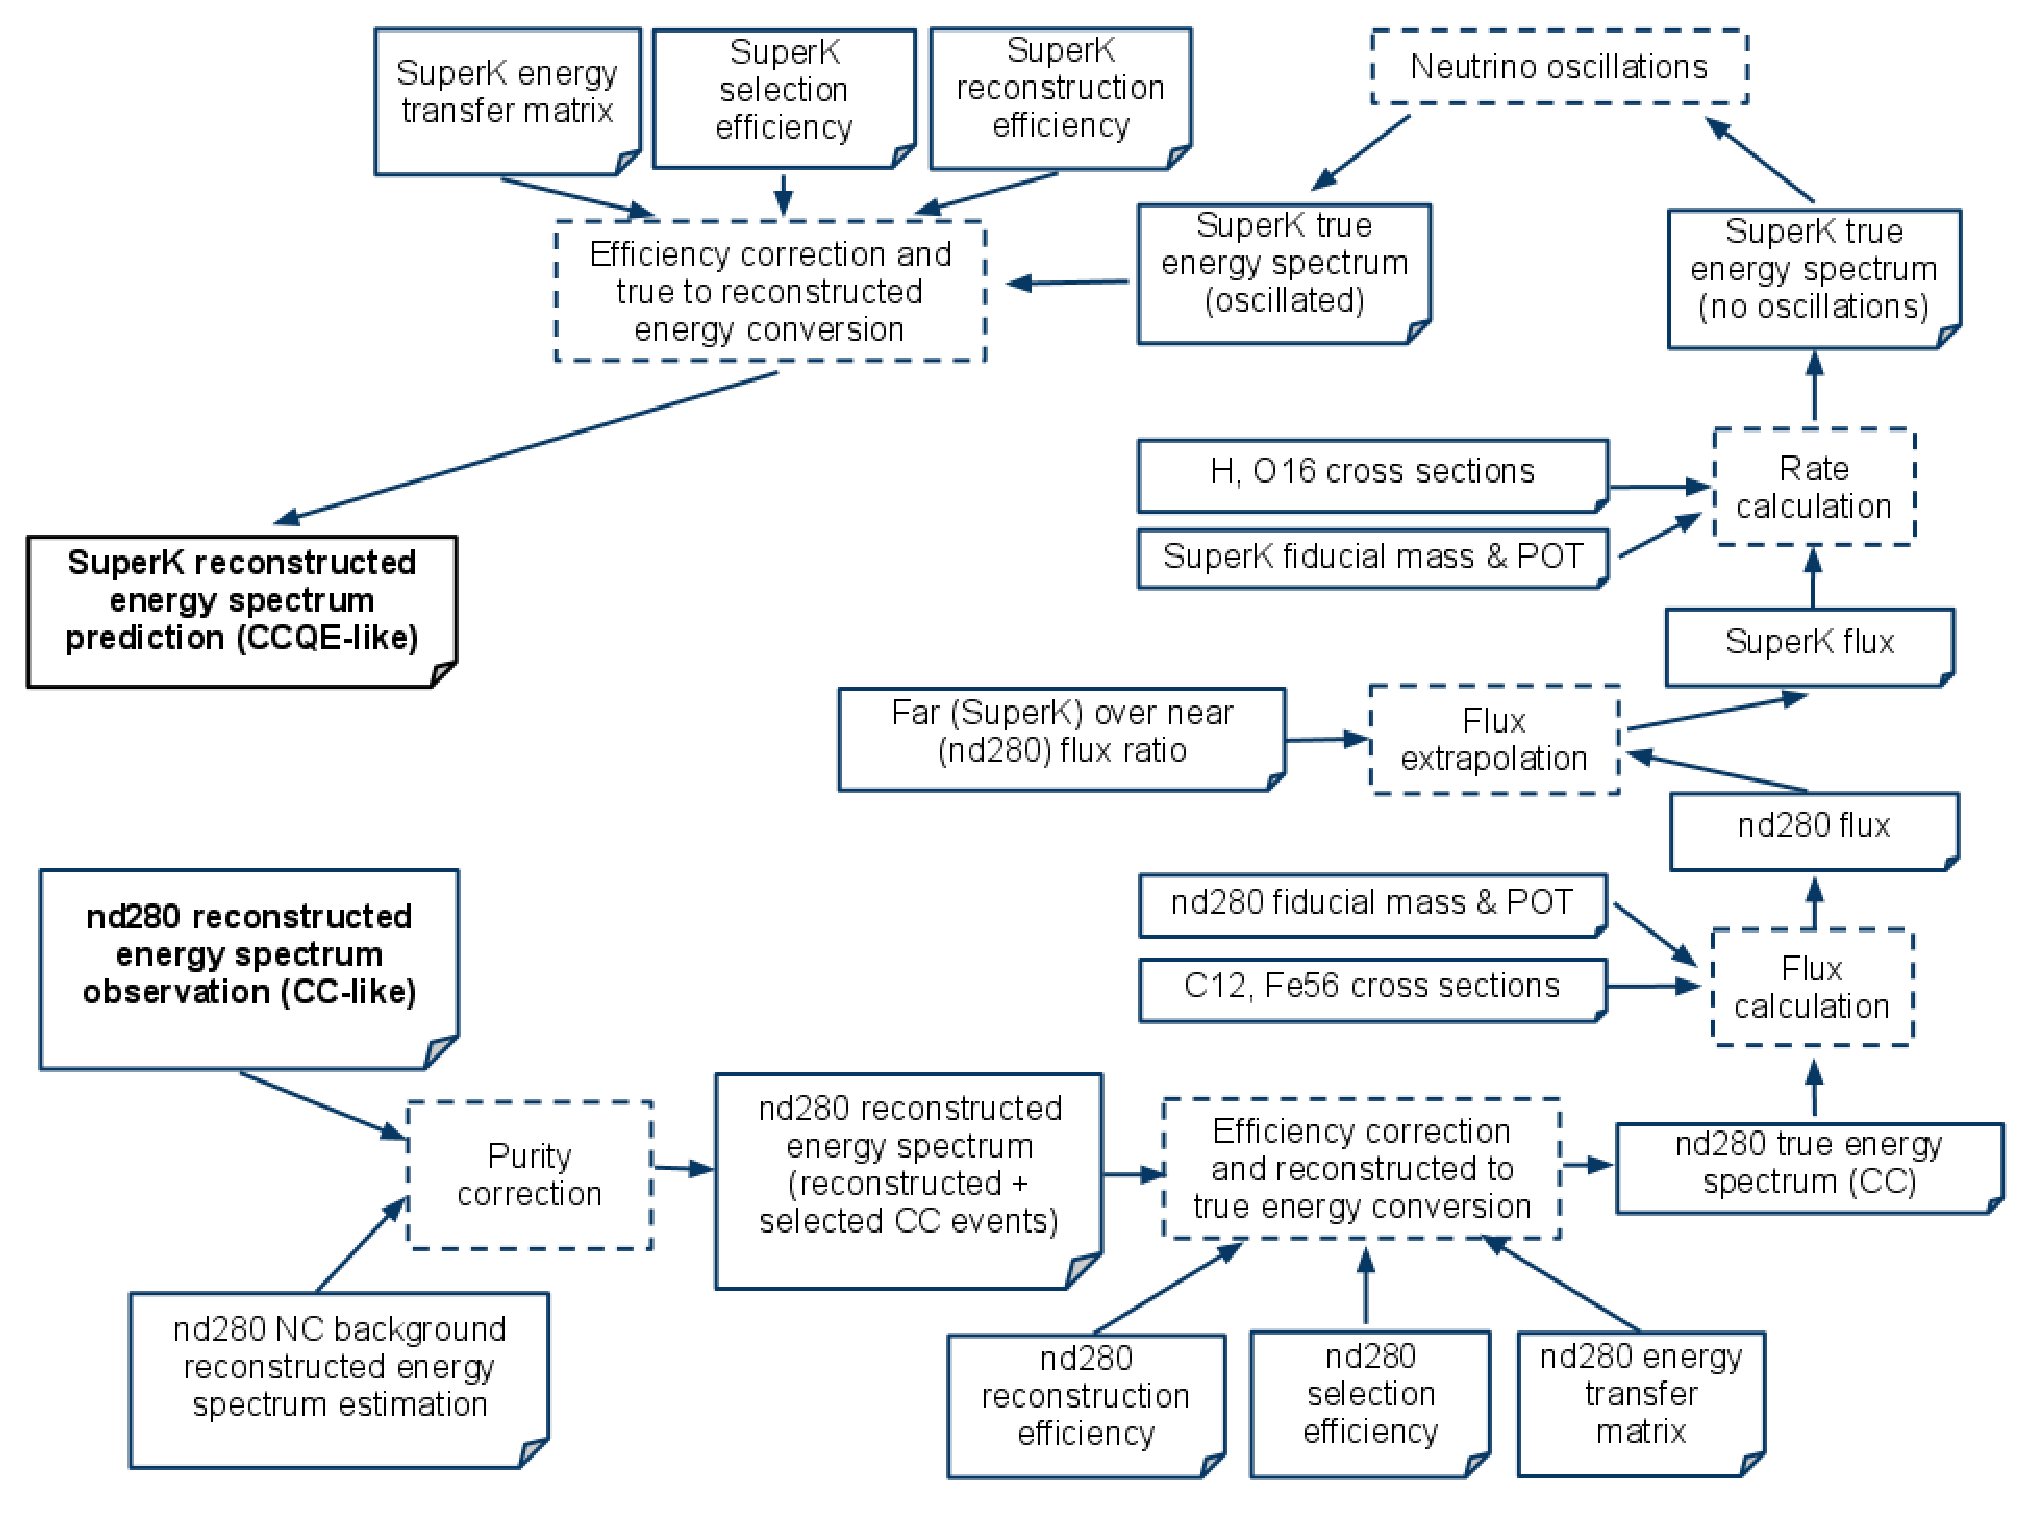
\includegraphics[width=38pc]{./images/analysis_steps.eps}
\caption{
  Outline of the procedure for predicting the SuperK reconstructed energy spectrum 
  of $\nu_{\mu}$ CCQE-like events
  from the $\nu_{\mu}$ CC inclusive reconstructed energy spectrum 
  measured in ND280.
}
\label{fig:AnalysisSteps}
\end{figure*}

The predicted reconstructed energy ($E_{r}$) spectrum ($\frac{dN_{SK}^{exp}}{dE_{r}}$) 
of selected 1 $\mu$-like ring events at SuperK,
is the sum of the corresponding spectra for all event types $m$\footnote{
 In this work, 
  $m$ = $\nu_{\mu}$ CCQE, $\nu_{\mu}$ CC1$\pi$, $\nu_{\mu}$ CC other, $\nu_{\mu}$($\nu_{\tau}$) NC, 
  $\bar{\nu_{\mu}}$ CCQE, $\bar{\nu_{\mu}}$ CC1$\pi$, $\bar{\nu_{\mu}}$ CC other $\bar{\nu_{\mu}}$($\bar{\nu_{\tau}}$) NC, 
  $\nu_{e}$ CCQE, $\nu_{e}$ CC1$\pi$, $\nu_{e}$ CC other and  $\nu_{e}$ NC.
} 
whose contribution is tracked separately.

\begin{equation}
\displaystyle
  \frac{dN_{SK}^{exp}(E_{r})}{dE_{r}} =
     \sum_{m} \frac{dN_{SK;m}^{exp}(E_{r})}{dE_{r}} 
\end{equation}

Let 
$\epsilon^{reco}_{SK;m}(E_{t})$
be the SuperK efficiency for reconstructing a neutrino event of type $m$ and true energy $E_{t}$, 
and 
$\epsilon^{sel}_{SK;m}(E_{r})$ be the SuperK efficiency for selecting an event of type $m$
and reconstructed energy $E_{r}$.
If $R_{SK;m}(E_{t},E_{r})$ is the SuperK energy transfer matrix\footnote{
The quantity $R_{SK;m}(E_{t},E_{r})$ is defined by
\begin{equation}
\displaystyle
   \frac{dN_{SK;m}}{dE_{r}}
 = \int { dE_{t} \frac{d^{2}N_{SK;m}}{dE_{r}dE_{t}} }
 = \int { dE_{t} \frac{dN_{SK;m}}{dE_{t}} R_{SK;m} }
\end{equation}
This implies that
\begin{equation}
\displaystyle
    R_{SK;m} 
 = \frac{d^{2}N_{SK;m}}{dE_{r}dE_{t}} / 
    \frac{dN_{SK;m}}{dE_{t}}
\end{equation}
This also defines the normalization properties all the $R_{SK;m}(E_{t},E_{r})$ matrix:
the elements for each $E_{r}$ row (or column, depending on how the matrix is represented) should add up to 1.
}
for events of type $m$, the expected reconstructed energy spectrum can be expressed in terms of the
total true neutrino energy spectrum
($\frac{dN_{SK;m}^{tot}(E_{t})}{dE_{t}}$):

\begin{equation}
\displaystyle
  \frac{dN_{SK}^{exp}(E_{r})}{dE_{r}} 
  = \sum_{m} \int dE_{t} 
    \frac{dN_{SK;m}^{tot}(E_{t})}{dE_{t}} 
    R_{SK;m}(E_{t},E_{r}) 
    \epsilon^{sel}_{SK;m}(E_{r}) 
    \epsilon^{reco}_{SK;m}(E_{t})
\end{equation}

The above expression can be rewritten to explicitly include
the survival probability $P_{m}^{surv}(E_{t})$ for neutrinos of energy $E_{t}$,
and the total non-oscillated true neutrino energy spectrum $\frac{dN_{SK;m}^{tot;unosc}}{dE_{t}}$:
\begin{equation}
\displaystyle
  \frac{dN_{SK}^{exp}(E_{r})}{dE_{r}} 
  = \sum_{m} \int dE_{t} 
    \frac{\displaystyle dN_{SK;m}^{tot;unosc}(E_{t})}
         {\displaystyle dE_{t}} 
    P_{m}^{surv}(E_{t}) 
    R_{SK;m}(E_{t},E_{r}) 
    \epsilon^{sel}_{SK;m}(E_{r}) 
    \epsilon^{reco}_{SK;m}(E_{t})
\end{equation}

The total non-oscillated true neutrino energy spectrum is related to
the estimated neutrino flux at SuperK
($\frac{d\Phi_{SK}(E_{t})}{dE_{t}}$) in the following way:
{
\arraycolsep=2pt
\begin{equation}
\displaystyle
\begin{array}{lcl}
  \frac{dN_{SK}^{exp}(E_{r})}{dE_{r}}  & = & 
    N_{SK}^{POT} M_{SK}^{fid} \frac{N_{A}}{A_{H20}}
    {\displaystyle \sum_{m} \int dE_{t}} \Bigg( 
    \frac{d\Phi_{SK}(E_{t})}{dE_{t}} \times \\ & &
    \sigma_{H20}^{tot}(E_{t}) 
    f_{m}(E_{t}) 
    P_{m}^{surv}(E_{t}) 
    R_{SK;m}(E_{t},E_{r}) 
    \epsilon^{sel}_{SK;m}(E_{r}) 
    \epsilon^{reco}_{SK;m}(E_{t}) \Bigg)
\end{array}
\label{eq:rate_sk}
\end{equation}
}
where 
$N_{SK}^{POT}$ is the proton-on-target exposure for the analyzed
SuperK data sample,
$M_{SK}^{fid}$ is the SuperK fiducial volume mass,
$\sigma_{H20}^{tot}(E_{t})$ is the total neutrino interaction cross section in water at energy $E_{t}$, 
$f_{m}(E_{t}$ is the fraction of events of type $m$,
$N_{A}$ is Avogadro's number and $A_{H20}$ is the water mass number.

The absolute neutrino flux $\frac{d\Phi_{SK}(E_{t})}{dE_{t}}$
in Eq. \ref{eq:rate_sk}, for which significant uncertainties exist,
can be constrained if it is expressed in terms of 
the observed reconstructed neutrino energy spectrum from an ND280 
inclusive charged-current sample.
From the definition of the far-over-near ratio

\begin{equation}
\displaystyle
  \frac{d\Phi_{SK}(E_{t})}{dE_{t}} = 
    R^{F/N}(E_{t}) \frac{d\Phi_{ND280}(E_{t})}{dE_{t}}
\end{equation}

where $\frac{d\Phi_{ND280}(E_{t})}{dE_{t}}$ is the neutrino flux at ND280.
This latter quantity can be related to the total CC true neutrino energy spectrum
$\frac{dN_{ND280;CC}^{tot}(E_{t})}{dE_{t}}$ as follows:

\begin{equation}
\displaystyle
  \frac{d\Phi_{SK}(E_{t})}{dE_{t}} = 
  \frac{R^{F/N}(E_{t}) A_{ND280}}{N_{ND280}^{POT} M_{ND280}^{fid} N_{A} \sigma^{CC}_{ND280}(E_{t})} 
  \frac{dN_{ND280;CC}^{tot}(E_{t})}{dE_{t}}
\end{equation}

where 
$N_{ND280}^{POT}$ is the proton-on-target exposure for the analyzed
ND280 data sample,
$M_{ND280}^{fid}$ is the fiducial mass for the ND280 `target' region, $\sigma^{CC}_{ND280}(E_{t})$ is the total 
charged-current cross section for the ND280 `target' region mixture at energy $E_{t}$
and $A_{ND280}$ is the mass number for the ND280 `target' mixture.

The total CC true neutrino energy spectrum can be expressed in terms
of the observed
reconstructed neutrino energy spectrum (which has the NC background subtracted):
{
\arraycolsep=2pt
\begin{equation}
\displaystyle
\begin{array}{lcl}
  \frac{d\Phi_{SK}(E_{t})}{dE_{t}} & = & 
  \frac{R^{F/N}(E_{t}) A_{ND280}}{N_{ND280}^{POT} M_{ND280}^{fid} \sigma^{CC}_{ND280}(E_{t})}
  {\displaystyle \int dE_{r\prime}} \Bigg( \\ & &
    \Big(
      \frac{dN_{ND280;CC-like}^{obs}(E_{r\prime})}{dE_{r\prime}} - 
      \frac{dN_{ND280;NC-bkg}^{exp}(E_{r\prime})}{dE_{r\prime}}
    \Big)  
    \frac{R^{T}_{ND280;CC}(E_{t},E_{r\prime})}
         {\epsilon^{reco}_{ND280;CC}(E_{t}) \epsilon^{sel}_{ND280;CC}(E_{r\prime})}
  \Bigg)
\end{array}
\label{eq:flux_sk}
\end{equation}
}
where
$\epsilon^{reco}_{ND280;CC}(E_{t})$ is the ND280 efficiency for reconstructing a charged-current neutrino event with true energy $E_{t}$,
$\epsilon^{sel}_{ND280;CC}(E_{r\prime})$ is the ND280 selection efficiency for a charged-current event reconstructed with energy $E_{r\prime}$, and
$R^{T}_{ND280;CC}(E_{t},E_{r\prime})$ is the transpose of the ND280 energy transfer matrix for charged-current events.

Combining Eq. \ref{eq:rate_sk} and \ref{eq:flux_sk} we obtain
{
\arraycolsep=2pt
\begin{equation}
\displaystyle
\begin{array}{lcl}
  \frac{dN_{SK}^{exp}(E_{r})}{dE_{r}} & = & 
  \frac{N_{SK}^{POT} M_{SK}^{fid} A_{ND280}}{N_{ND280}^{POT} M_{ND280}^{fid} A_{H20}} 
  {\displaystyle \sum_{m} \int dE_{t} \int dE_{r\prime}} \Bigg( 
  R^{F/N}(E_{t})
  \frac{\sigma_{H20}^{tot}(E_{t}) f_{m}(E_{t})}{\sigma^{CC}_{ND280}(E_{t})}
  P_{m}^{surv}(E_{t}) \times \\ & &
  \Big(\frac{dN_{ND280;CC-like}^{obs}(E_{r\prime})}{dE_{r\prime}} - 
       \frac{dN_{ND280;NC-bkg}^{exp}(E_{r\prime})}{dE_{r\prime}}\Big)  \times \\ & &
    R_{SK;m}(E_{t},E_{r}) R^{T}_{ND280;CC}(E_{t},E_{r\prime}) 
    \frac{\epsilon^{sel}_{SK;m}(E_{r}) \epsilon^{reco}_{SK;m}(E_{t})}
         {\epsilon^{reco}_{ND280;CC}(E_{t}) \epsilon^{sel}_{ND280;CC}(E_{r\prime})} 
    \Bigg)
\end{array}
\label{eq:far_prediction}
\end{equation}%
}

%
% Implementation / analysis specifics
%

\subsection {3.23$\times10^{19}$-POT analysis specifics and discussion of ND280 input}
\label{sec:superkprediction_analysis_specifics}

In the present analysis, there is no spectral information in the inclusive CC ND280 measurement.
In this case, Eq. \ref{eq:far_prediction} simplifies to
\begin{equation}
\displaystyle
\begin{array}{lcl}
  \frac{dN_{SK}^{exp}(E_{r})}{dE_{r}}  & = & 
    N_{SK}^{POT} M_{SK}^{fid} \frac{N_{A}}{A_{H20}}
    C_{ND280}
    {\displaystyle \sum_{m} \int dE_{t}} \Bigg( 
    \\ & &
    \frac{d\Phi_{SK}(E_{t})}{dE_{t}} 
    \sigma_{H20}^{tot}(E_{t}) 
    f_{m}(E_{t}) 
    P_{m}^{surv}(E_{t}) 
    R_{SK;m}(E_{t},E_{r}) 
    \epsilon^{sel}_{SK;m}(E_{r}) 
    \epsilon^{reco}_{SK;m}(E_{t}) \Bigg)
\end{array}
\label{eq:far_prediction_no_nd280_spectrum}
\end{equation}
where $C_{ND280}$ is the ND280 data-driven correction factor on the flux times cross section product.
We note that the far over near ratio $R^{F/N}(E_{t})$, discussed previously, does not appear in the above formula.
This follows from the fact that the ND280 measurement has no energy dependence.

In Eq. \ref{eq:far_prediction_no_nd280_spectrum}, $C_{ND280}$ is given by
\begin{equation}
\displaystyle
  C_{ND280} = 
    \frac{N^{obs}_{ND280;CC-like}}
         {N^{exp}_{ND280;CC}+N^{exp}_{ND280;NC-bkg}}
\label{eq:nd280correction}
\end{equation}
where
$N^{obs}_{ND280;CC-like}$ is the observed number of CC-like events,
$N^{exp}_{ND280;NC-bkg}$ is the expected NC contamination of the observation, and
$N^{exp}_{ND280;CC}$ is the expected number of CC events.

In the present analysis 
$C_{ND280}$ is 1.1549 for GENIE and 1.06127 for NEUT\cite{ND280AnalysisInputs,ND280ClaudioThesis}.
The difference in the required correction factor for GENIE and NEUT reflects 
generator-level tuning choices; mainly, it reflects the dramatic difference in the choice of the input CCQE axial mass.
The authors of GENIE use a value of $M_{A}$ = 0.99 GeV/$c^{2}$ which is better-motivated theoretically.
One the other hand, the authors of NEUT use a higher value ($M_{A}$ = 1.2 GeV/$c^{2}$) 
motivated by K2K and MiniBooNE measurements of an increased event rate (in $C^{12}$, $O^{16}$ targets)
compared with expectations informed by previous measurements in deuterium targets (although the observed excess
is only about 1$\sigma$). It is plausible, although not satisfying, that $M_{A}$ should have a larger
values for nuclear targets. However, it is also likely that the discrepancy is caused, amongst other things, 
by underestimating the K2K and MiniBooNE neutrino flux,
or by the existence of unmodelled CCQE-like contributions (2p2h).
So, increasing $M_{A}$ may or may not be appropriate.
The issue is far from being resolved and reflects a genuine physics uncertainty: 
the absolute neutrino cross section at around 1 GeV is known only to about 20-30\%.

In any case, this (or any) T2K oscillation analysis is credible only if it is 
shown explicitly that it does not depend on semi-arbitrary generator choices,
and that measurements from the near detector suite effectively constrain uncertainties 
in the product of flux and cross-section. It also needs to be shown that any difference in
the oscillation results is well-understood in terms of the quoted cross-section systematics.
This is the main motivation behind pursuing this analysis using both GENIE and NEUT.


\subsection {Implementation details}

So far, the SuperK spectrum prediction method has been presented in a formal manner.
In practice, the procedure for calculating the spectrum can be simplified.
By using appropriate Monte Carlo `templates', representing the simulated number of
events in N-dimensional bins of kinematical quantities,
one can avoid performing integrations such as the one appearing 
in Eq. \ref{eq:rate_sk}\footnote
{
  On the SuperK side of the calculation, 
  avoiding integrations such as the one in Eq. \ref{eq:rate_sk} using MC templates
  is just a matter of convenience and computational efficiency.
  However, on the ND280 side, avoiding such integrations and, instead, using MC templates 
  is a necessity.
  Indeed, for ND280, event rate calculations folding in the flux and neutrino cross section to
  should be generalized to take into account the effects arising from the convolution of a 
  non-uniform flux with non-uniform detector mass distribution. In this case, the event rate
  can be written as
  \begin{equation}
    \displaystyle
       N^{exp} = N^{POT} N_{A} 
            \int d^{3}x \int d^{3}p 
            \frac{d^{6}\Phi({\bf x},{\bf p})}{d^{3}xd^{3}p} 
            \epsilon(E) 
            \sum_{a} \frac{\sigma_{a}(E)}{A_{a}} \int dl\rho_{a}
       \label{eq:event_rate_complex}
  \end{equation}
  where 
  the vector ${\bf x}$ is the flux neutrino point of origin and
  the vector ${\bf p}$ is the flux neutrino momentum.
  In the above equation, the sum over $a$ is the sum over nuclear targets in the detectors.
  The mass number of each nuclear target is $A_{a}$ and the total interaction cross section is $\sigma_{a}(E)$.
  The final integral in Eq. \ref{eq:event_rate_complex} calculates the density-weighted path length
  for nuclear target $a$ with density $\rho_{a}$ along the given flux netrino trajectory.
  This complicated integration is already performed by GENIE and NEUT using Monte Carlo techniques
  and the result is built into the generated templates.
  It is practically impossible and unnecessary to reproduce this time-consuming Monte Carlo
  integration in the context of the oscillation analysis.
}

In this analysis, 
oscillation parameters are determined by fitting the reconstructed energy ($E_{r}$) spectrum
of 1-ring $\mu$-like events observed at SuperK, 
oscillation weights are functions of the true energy ($E_{t}$),
and all considered systematics affecting the SuperK spectrum prediction
either have no kinematical dependence or depend 
on only one of true or reconstructed energy.
Therefore, in the context of this analysis, it is sufficient to use 2-dimensional
templates representing the number of SuperK events, as estimated by MC,
as functions of $E_{r}$ and $E_{t}$.
Let $N_{SK;m;r;t}^{MC}$ be such a template for events of mode $m$ in the 1 $\mu$-like ring sample,
where indices $r$ and $t$ denote, respectively, reconstructed and true energy bin numbers.
The construction of these templates is discussed in detail in Sec. \ref{sk_templates}.
The predicted number $N_{SK;r}^{exp}$ 
of SuperK events in the $r^{th}$ reconstructed energy bin
can be written in terms of the $N_{SK;m;r;t}^{MC}$ templates as
\begin{equation}
\displaystyle
  N_{SK;r}^{exp} = 
    C_{ND280}
    \sum_{m} \sum_{t} 
    	P_{m;t}^{surv}
	N_{SK;m;r;t}^{MC}
\label{eq:far_prediction_no_nd280_spectrum_with_sk_templates}
\end{equation}
where $C_{ND280}$ is the ND280 correction factor defined in Eq. \ref{eq:nd280correction}
and $P_{m;t}^{surv}$ is oscillation survival probability applied in the $t^{th}$ true energy
bin of the SuperK MC template which corresponds to mode $m$.
Application of term $P_{m;t}^{surv}$ is discussed in Sec. \ref{applying_oscillations}.

Only the value of $C_{ND280}$ is needed for the prediction of the nominal SuperK spectrum.
However, for systematic studies, one needs to be able to calculate how the value of $C_{ND280}$ 
is modified as a result of systematic parameter variations.
Therefore it is necessary to express $C_{ND280}$ in terms of appropriate ND280 MC templates.
In this analysis, all considered systematics affecting $C_{ND280}$
either have no kinematical dependence or depend on true energy only.
Therefore, in the context of this analysis, it is sufficient to use 1-dimensional
templates representing the number of ND280 events, as estimated by MC,
as functions of $E_{t}$.
Let $N_{ND280;m\prime;t}^{MC}$ be such a template for events of mode $m\prime$ in the
ND280 CC inclusive sample, where index $t$ denotes true energy bin number.
The construction of these templates is discussed in Sec. \ref{nd280_templates}.
Using the ND280 MC templates, $C_{ND280}$ can be written as
\begin{equation}
\displaystyle
  C_{ND280} = N^{obs}_{ND280;CC-like} / \sum_{m\prime} N^{MC}_{ND280;m\prime}
\label{eq:nd280correction_with_templates}
\end{equation}

Using Eq. \ref{eq:nd280correction_with_templates}, 
Eq. \ref{eq:far_prediction_no_nd280_spectrum_with_sk_templates} can be written as
\begin{equation}
\displaystyle
  N_{SK;r}^{exp} = 
    (N^{obs}_{ND280;CC-like} /
     \sum_{m\prime} N^{MC}_{ND280;m\prime})
    \cdot 
    \sum_{m} \sum_{t} 
    	P_{m;t}^{surv}
	N_{SK;m;r;t}^{MC}
\label{eq:far_prediction_no_nd280_spectrum_final}
\end{equation}
This is the actual formula used in this analysis for predicting the 
SuperK reconstructed energy spectrum.

\subsection{Construction of SuperK MC templates}
\label{sk_templates}

The $N_{SK;m;r;t}^{MC}$ templates are shown in Fig. \ref{fig:genie_etrue_ereco_templates} (GENIE) 
and Fig. \ref{fig:neut_etrue_ereco_templates} (NEUT). Separate templates are used for
$\nu_{\mu}$ CCQE\footnote{
  A commonly asked question is why the $\nu_{\mu}$-CCQE template is not just a `line' along
  the diagonal. Conservation of energy and momentum is the anwer to this question.
  Recall that the $\nu_{\mu}$-CCQE template is generated from a sample of $\nu_{\mu}$ interactions
  in water and that, in oxygen, the Fermi level $k_{F}$ is 225 MeV.
  On the other hand, recall that the hit bound-nucleon momentum is `esoteric' 
  and that the reconstructed neutrino energy formula naturally assumes that the hit nucleon was at rest.
}, 
$\nu_{\mu}$ CC1$\pi$, 
$\nu_{\mu}$ CC other, 
$\nu_{\mu}$($\nu_{\tau}$) NC, 
$\bar{\nu_{\mu}}$ CCQE, 
$\bar{\nu_{\mu}}$ CC1$\pi$, 
$\bar{\nu_{\mu}}$ CC other, 
$\bar{\nu_{\mu}}$($\bar{\nu_{\tau}}$) NC, 
$\nu_{e}$ CCQE, 
$\nu_{e}$ CC1$\pi$,
$\nu_{e}$ CC other and 
$\nu_{e}$ NC.
The events contributing to the construction of these 2-D templates are the ones that
pass the `1-ring $\mu$-like (tight)' cuts. The templates span the 0-10 GeV range in
both $E_{r}$ and $E_{t}$ variables using 50 MeV bins.

The templates were generated using the 2010a GENIE and NEUT SuperK samples and
then they were reweighted to the 2010d(v2) flux \cite{BeamWeights10dv2}.
Details of the 2010a GENIE and NEUT SuperK samples and of the applied selection cuts are given below.

\subsubsection*{SuperK MC samples}

\begin{itemize}
\item
GENIE SuperK sample:\\
 The 2010a GENIE SuperK Monte Carlo sample was generated at the Rutherford Appleton Laboratory
 PPD Tier2 cluster using GENIE v2.6.0 and the 2010a JNUBEAM flux \cite{BeamFlux10a}.
 The GENIE decay flags for $D^{+}$, $D^{-}$, $D^{0}$, $\bar{D^{0}}$, $D_{s}^{+}$, $D_{s}^{-}$,
 $\Lambda_{c}^{+}$, $\Sigma_{c}^{0}$, $\Sigma_{c}^{+}$ and $\Sigma_{c}^{++}$ 
 were set to `true' (non-default GENIE settings) as the SuperK detector simulation would not
 decay charmed hadrons. Default GENIE v2.6.0 values were used for all other physics options.

 The GENIE vector files were proccessed by P. de Perio at the SciNet cluster in Toronto.
 The SK software used is the same as that used for the official 10a NEUT production
 (SKDETSIM-v11p79\_for\_atmnu\_apr10, ATMPD-10a, SKOFL-10a, ROOT-v5.26) \cite{PatrickPrivComm}.
 The `T2K PMT flasher reduction' cut was not included when filling the output DSTs.
 According to experts `this is a small effect ( $<$ 1\% )' \cite{SuperKFC}.

 Using the GENIE v2.6.0 cross section calculations for water and the 2010a JNUBEAM flux,
 we calculate
 1325.4200 $\nu_{\mu}$       events / 22.5 kt fiducial mass / $10^{21}$ POT,
   65.1023 $\bar{\nu_{\mu}}$ events / 22.5 kt fiducial mass / $10^{21}$ POT and
   25.9600 beam $\nu_{e}$    events / 22.5 kt fiducial mass / $10^{21}$ POT.
 After applying fiducial volume cuts to the generated samples, we find that
   604403 $\nu_{\mu}$,
   303747 $\bar{\nu_{\mu}}$ and
   621525 beam $\nu_{e}$  
 events have survived.
 From the above, we calculate the following absolute normalizations 
 for the 2010a samples:
   4.560000$\times10^{23}$ POT for the $\nu_{\mu}$ sample,
   4.665680$\times10^{24}$ POT for the $\bar{\nu_{\mu}}$ sample and
   2.394164$\times10^{25}$ POT for the beam $\nu_{e}$ sample.
 Therefore, the MC scaling factors to the data beam exposure ($3.23\times10^{19}$ POT) are
   7.08333$\times10^{-5}$ ($\nu_{\mu})$,
   6.92289$\times10^{-6}$ ($\bar{\nu_{\mu}}$),
   1.34911$\times10^{-6}$ (beam $\nu_{e}$). 
   
\item
NEUT SuperK sample:\\
 The 2010a NEUT SuperK Monte Carlo sample was generated and processed at the Kamioka cluster.
 NEUT v5.0.7 and the 2010a JNUBEAM flux were used.
 The corresponding SuperK DSTs were kindly provided by P. de Perio.
 The MC scaling factors to the data POT exposure are the ones provided by Y.Hayato and J.Kameda \cite{KamedaPrivComm}:
   7.35361$\times10^{-5}$ ($\nu_{\mu})$,
   7.17816$\times10^{-6}$ ($\bar{\nu_{\mu}}$),
   1.48428$\times10^{-6}$ (beam $\nu_{e}$). 

\end{itemize}

\subsubsection*{SuperK selection cuts}

The standard SuperK cuts for obtaining
a) `fully contained fiducial volume (FCFV)',
b) `1 $\mu$-like ring',
c) `1 $\mu$-like ring (tight)' and
d) `$>$ 1 $\mu$-like ring'
samples are shown in Tab. \ref{tab:NuMuEventSelections}.
In this analysis, the 1 $\mu$-like ring (tight) event selection is used.

\begin{table}
\centering
\begin{tabular}{| c | c | c | c |}
\hline
Fully contained & 1 $\mu$-like ring & 1 $\mu$-like ring & $>$ 1 $\mu$-like ring  \\
fiducial volume &  & (tight) & \\
\hline
\hline
Number of PMT hits  & Number of PMT hits  &  Number of PMT hits  &  Number of PMT hits \\
in highest charge   & in highest charge   &  in highest charge   &  in highest charge  \\
Outer Detector      & Outer Detector      & Outer Detector       & Outer Detector      \\
cluster $<$= 15     & cluster $<$= 15     & cluster $<$= 15      & cluster $<$= 15     \\
\hline
Vertex $>$ 2m from  & Vertex $>$ 2m from  & Vertex $>$ 2m from   & Vertex $>$ 2m from  \\
Inner Detector wall & Inner Detector wall & Inner Detector wall  & Inner Detector wall \\
\hline
E$_{visible}$ $>$ 30 MeV & E$_{visible}$ $>$ 30 MeV & E$_{visible}$ $>$ 30 MeV & E$_{visible}$ $>$ 30 MeV \\
\hline
  & Exactly 1 ring & Exactly 1 ring & $>$ 1 ring \\
\hline
 & ip[0] = 3 & ip[0] = 3 & Ring with largest \\
 & ($\mu$-like ring) & ($\mu$-like ring) & amome is $\mu$-like \\
\hline
 &  & amomm[0] $>$ & \\
 &  & 200 MeV & \\
\hline
 &  & $<$= 1 decay e$^{-}$  & \\
\hline
\end{tabular}
\caption{
 Standard SuperK $\nu_{\mu}$ event selection cuts. In this analysis, the 1-ring $\mu$-like (tight) event selection is used.
 Potential benefits from including the multi-ring $\mu$-like events will be explored in future revision
 of this work.
}
\label{tab:NuMuEventSelections}
\end{table}

\begin{figure*}[htb]
\center
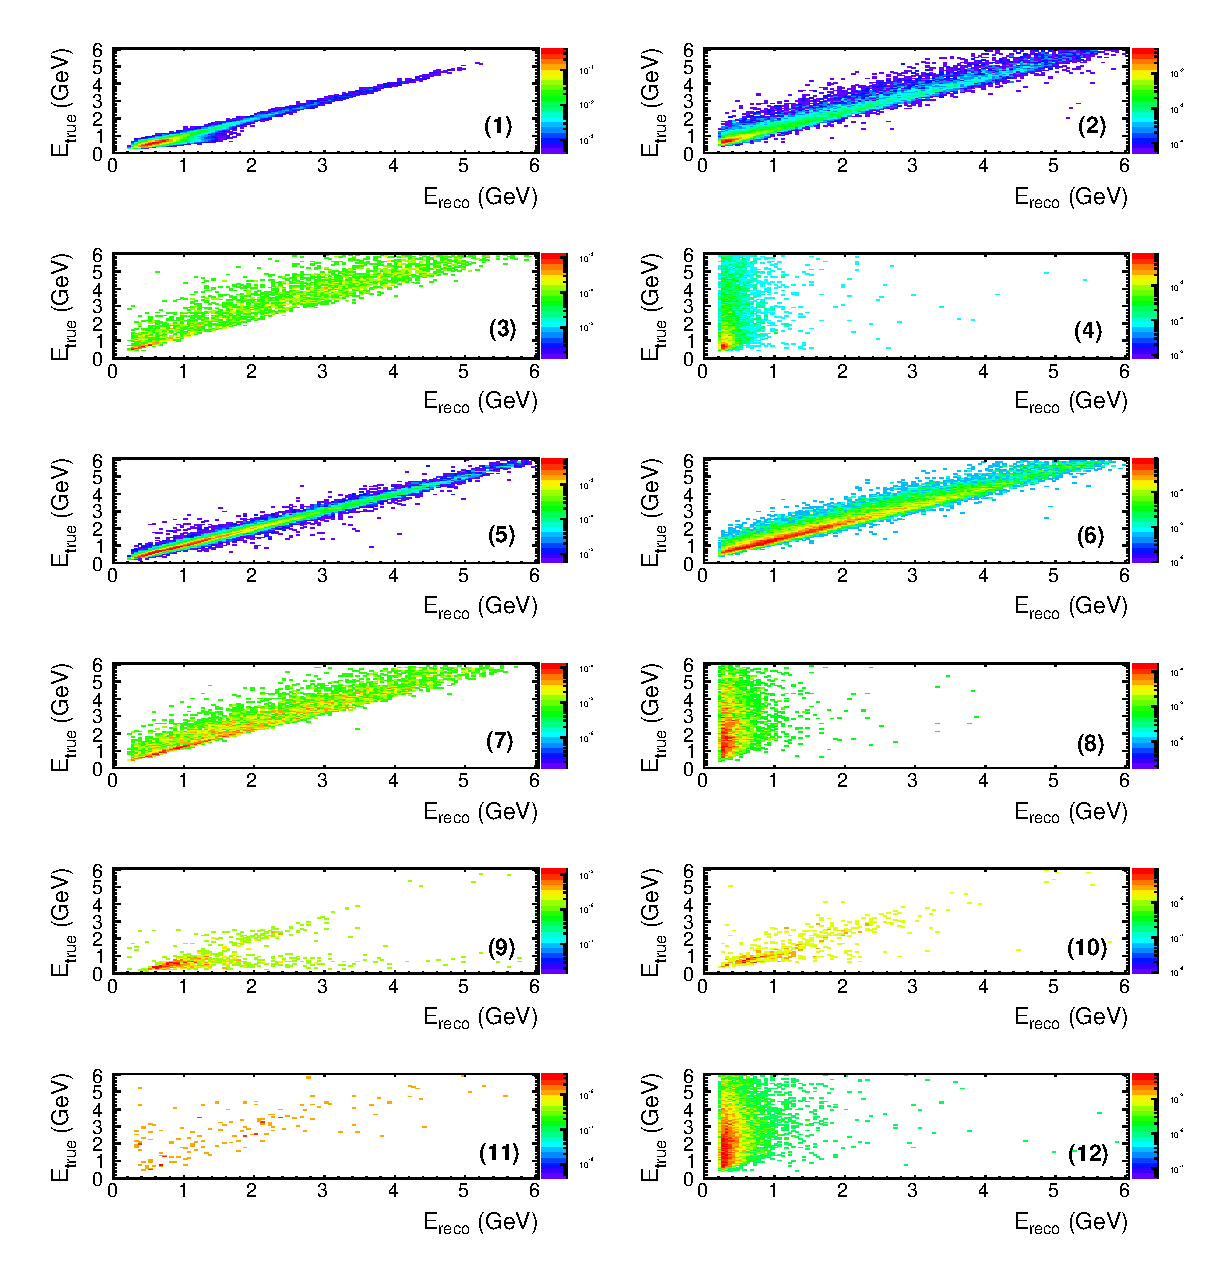
\includegraphics[width=38pc]{./images/templates/genie_etrue_ereco_templates.eps}
\caption{
  GENIE ($E_{t}$, $E_{r}$) 1-ring $\mu$-like MC templates. 
  The templates are shown for
  $\nu_{\mu}$ CCQE (1), 
  $\nu_{\mu}$ CC1$\pi$ (2), 
  $\nu_{\mu}$ CC other (3), 
  $\nu_{\mu}$($\nu_{\tau}$) NC (4), 
  $\bar{\nu_{\mu}}$ CCQE (5), 
  $\bar{\nu_{\mu}}$ CC1$\pi$ (6), 
  $\bar{\nu_{\mu}}$ CC other (7), 
  $\bar{\nu_{\mu}}$($\bar{\nu_{\tau}}$) NC (8), 
  $\nu_{e}$ CCQE (9),
  $\nu_{e}$ CC1$\pi$ (10),
  $\nu_{e}$ CC other (11) and
  $\nu_{e}$ NC (12).
  The templates are zoomed-in for illustration purposes. 
  The range 0-10 GeV is used in the analysis.
}
\label{fig:genie_etrue_ereco_templates}
\end{figure*}

\begin{figure*}[htb]
\center
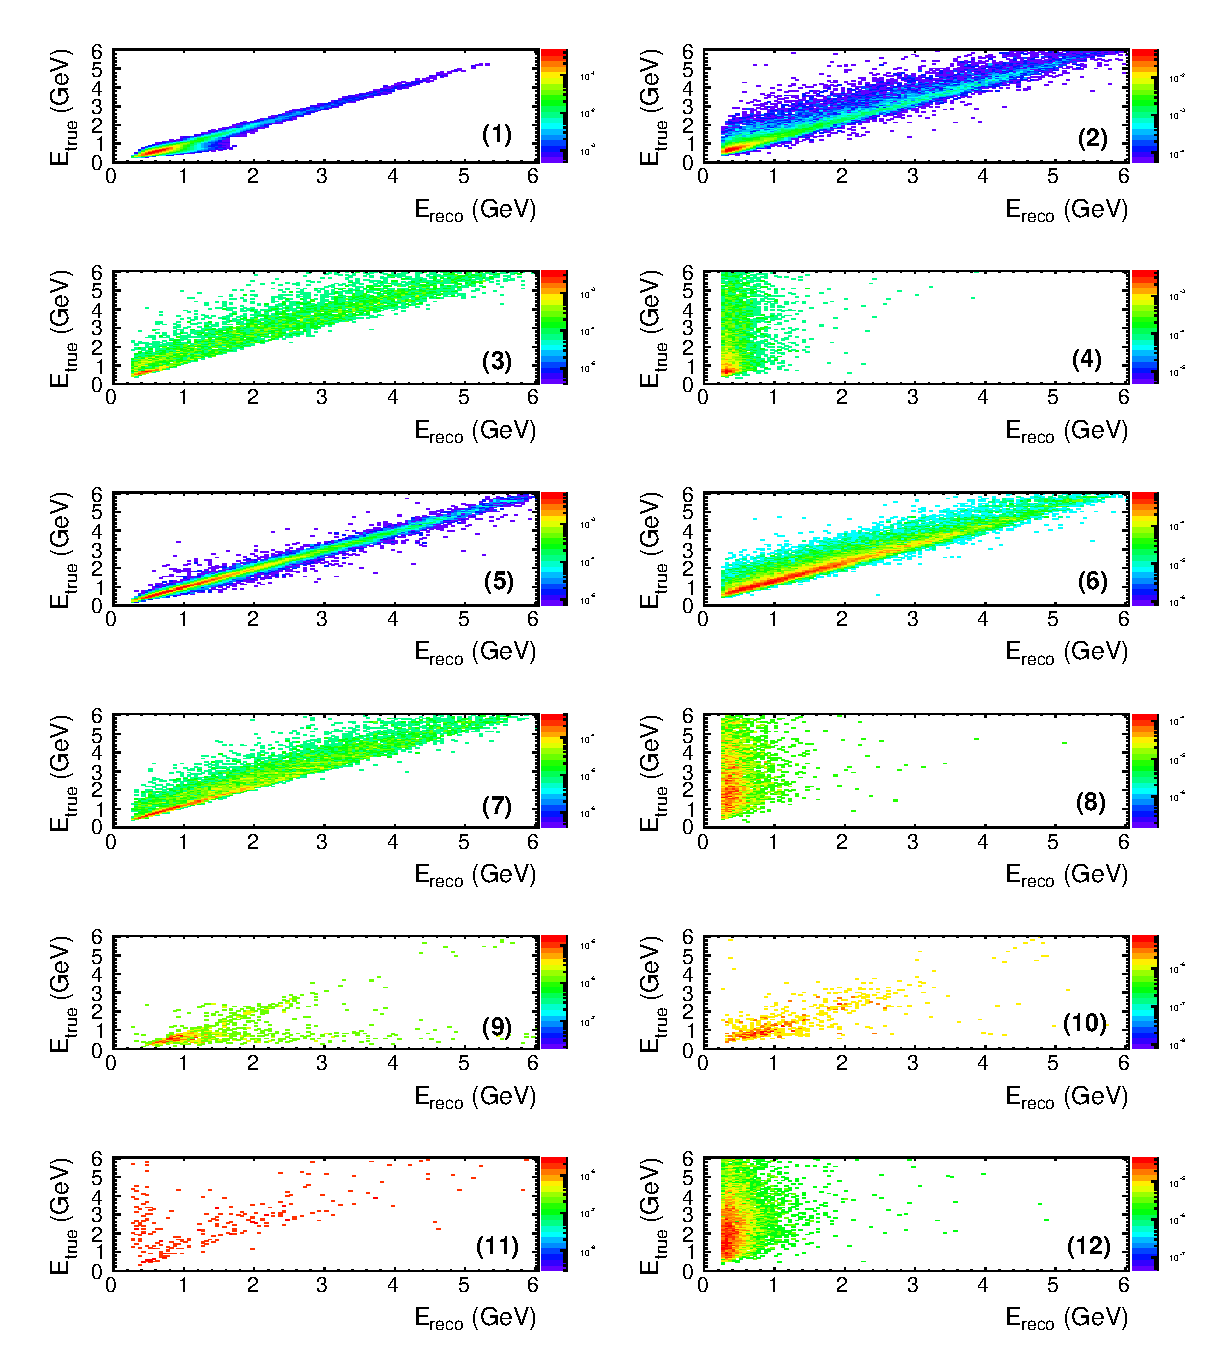
\includegraphics[width=38pc]{./images/templates/neut_etrue_ereco_templates.eps}
\caption{
  NEUT ($E_{t}$, $E_{r}$) 1-ring $\mu$-like MC templates. 
  The order of templates is the same as in Fig.\ref{fig:genie_etrue_ereco_templates}.
}
\label{fig:neut_etrue_ereco_templates}
\end{figure*}


\subsection{ND280 MC templates}
\label{nd280_templates}

The ND280 MC templates were provided directly by the ND280 group \cite{ND280AnalysisInputs}.
In total 21 histograms were provided representing the number of events as a function
of true energy for
1)  $\nu_{\mu}$ CC QE,	
2)  $\nu_{\mu}$ CC resonance,
3)  $\nu_{\mu}$ CC coherent,
4)  $\nu_{\mu}$ CC other,
5)  $\nu_{\mu}$ NC resonance,
6)  $\nu_{\mu}$ NC coherent,
7)  $\nu_{\mu}$ NC other,
8)  $\bar{\nu_{\mu}}$ CC QE,
9)  $\bar{\nu_{\mu}}$ CC resonance,
10) $\bar{\nu_{\mu}}$ CC coherent,
11) $\bar{\nu_{\mu}}$ CC other,
12) $\bar{\nu_{\mu}}$ NC resonance,
13) $\bar{\nu_{\mu}}$ NC coherent,
14) $\bar{\nu_{\mu}}$ NC other,
15) $\nu_{e}$ CC QE,
16) $\nu_{e}$ CC resonance,
17) $\nu_{e}$ CC coherent,
18) $\nu_{e}$ CC other,
19) $\nu_{e}$ NC resonance,
20) $\nu_{e}$ NC coherent and
21) $\nu_{e}$ NC other.
These templates were generated by applying the Saclay CC inclusive selection cuts
to the ND280 MCP1 GENIE and NEUT samples. The GENIE and NEUT versions used in the
ND280 MCP1 production are the same as those used at the SuperK 2010a production.
They were reweighted to the 2010d(v2) flux \cite{BeamWeights10dv2}.
More details are given in \cite{ND280AnalysisInputs}.

\subsection{Applying neutrino oscillations}
\label{applying_oscillations}

Oscillations are applied to the 
$\nu_{\mu}$-CCQE, $\nu_{\mu}$-CC1$\pi$, $\nu_{\mu}$-CCother, 
$\bar{\nu_{\mu}}$-CCQE, $\bar{\nu_{\mu}}$-CC1$\pi$ and $\bar{\nu_{\mu}}$-CCother
MC templates (as function of $E_{t}$).
Oscillations are not applied to the $\nu_{\mu}$-NC and $\bar{\nu_{\mu}}$-NC MC templates
since they serve as proxies for the $\nu_{\mu}(+\nu_{\tau})$-NC and $\bar{\nu_{\mu}}(+\bar{\nu_{\tau}})$-NC MC templates
which are unchanged under 
$\nu_{\mu} \rightarrow \nu_{\tau}$ and 
$\bar{\nu_{\mu}} \rightarrow \bar{\nu_{\tau}}$ oscillations.
We neglect contributions from $\nu_{\tau}$-CC and $\bar{\nu_{\tau}}$-CC as their
energy threshold is around 3.5 GeV and their effect is negligible.
The effect of sub-dominant (and unknown) $\nu_{e}$ oscillation is also neglected.
The following oscillation survival probability is applied:
\begin{equation}
\displaystyle
  P_{surv} = 1 - sin^{2}{2\theta_{23}} \cdot 
                 sin^{2}\Big(
                  1.267 \cdot \frac{\Delta m^{2}_{23} (eV^{2}/c^{4}) \cdot 295.335 (km)}{E_{t} (GeV)}
                 \Big)
\label{eq:osc_formula}
\end{equation}
The same $sin^{2}{2\theta_{23}}$ and $\Delta m^{2}_{23}$ parameters 
are used for both $\nu_{\mu}$ and $\bar{\nu_{\mu}}$ oscillations.


%
% Event numbers
%

\clearpage

\subsection{Nominal GENIE and NEUT expectations under various oscillation hypotheses}

In this section we present plots and tables comparing the GENIE and NEUT SuperK predictions
(after extrapolation) under various oscillation hypotheses.
Figs. \ref{fig:genie_mode_contrib_noosc} and \ref{fig:neut_mode_contrib_noosc} show,
respectively, the GENIE and NEUT
predicted (after extrapolation) non-oscillated reconstructed-energy spectrum of 1-ring $\mu$-like events 
passing the tight cuts (see Tab. \ref{tab:NuMuEventSelections}). 
The contributions from various true neutrino reaction modes are also shown. 
The corresponding oscillated predictions 
($sin^{2}2\theta_{23}$=1.0 and $\Delta m^{2}_{23}$=2.4$\times10^{-3}$ $eV^{2}/c^{4}$)
are shown in 
Fig. \ref{fig:genie_mode_contrib_2p4Em3_1p0} for GENIE and 
Fig. \ref{fig:neut_mode_contrib_2p4Em3_1p0} for NEUT.
In Tab. \ref{tab:genie_neut_mode_contrib} we summarize 
Figs. \ref{fig:genie_mode_contrib_noosc} - \ref{fig:neut_mode_contrib_2p4Em3_1p0}.

In Fig. \ref{fig:genie_sk_spectrum_twk_sinsq2theta} we show the GENIE predicted 1-ring $\mu$-like event
reconstructed energy spectrum (after extrapolation) for a fixed $\Delta m^{2}_{23}$ and various $sin^{2}2\theta_{23}$ values.
The corresponding plot for NEUT is shown in Fig. \ref{fig:neut_sk_spectrum_twk_sinsq2theta}.
Tab. \ref{tab:genie_neut_nsk_twk_sinsq2theta} 
summarizes Figs. \ref{fig:genie_sk_spectrum_twk_sinsq2theta} and \ref{fig:neut_sk_spectrum_twk_sinsq2theta}.
In Fig. \ref{fig:genie_sk_spectrum_twk_dmsq} we show the GENIE predicted 1-ring $\mu$-like event
reconstructed energy spectrum (after extrapolation) for a fixed $sin^{2}2\theta_{23}$ and various $\Delta m^{2}_{23}$ values.
The corresponding plot for NEUT is shown in Fig. \ref{fig:neut_sk_spectrum_twk_dmsq}.
Tab. \ref{tab:genie_neut_nsk_twk_dmsq}
summarizes Figs. \ref{fig:genie_sk_spectrum_twk_dmsq} and \ref{fig:neut_sk_spectrum_twk_dmsq}.

In Fig. \ref{fig:genie_nsk_osc_param_grid} we show the GENIE predicted integrated number 
of 1-ring $\mu$-like events (after extrapolation) for a grid of $sin^{2}2\theta_{23}$ and $\Delta m^{2}_{23}$ values.
The corresponding plot for NEUT is shown in Fig. \ref{fig:neut_nsk_osc_param_grid}.
Finally, in Fig. \ref{fig:genie_neut_nsk_difference_osc_param_grid} we show
(for the same grid of $sin^{2}2\theta_{23}$ and $\Delta m^{2}_{23}$ values)
the percentage difference of the NEUT and GENIE predictions of integrated number 
of 1-ring $\mu$-like events (after extrapolation).


\begin{figure}[ht]
\begin{minipage}[t]{0.48\linewidth}
\centering
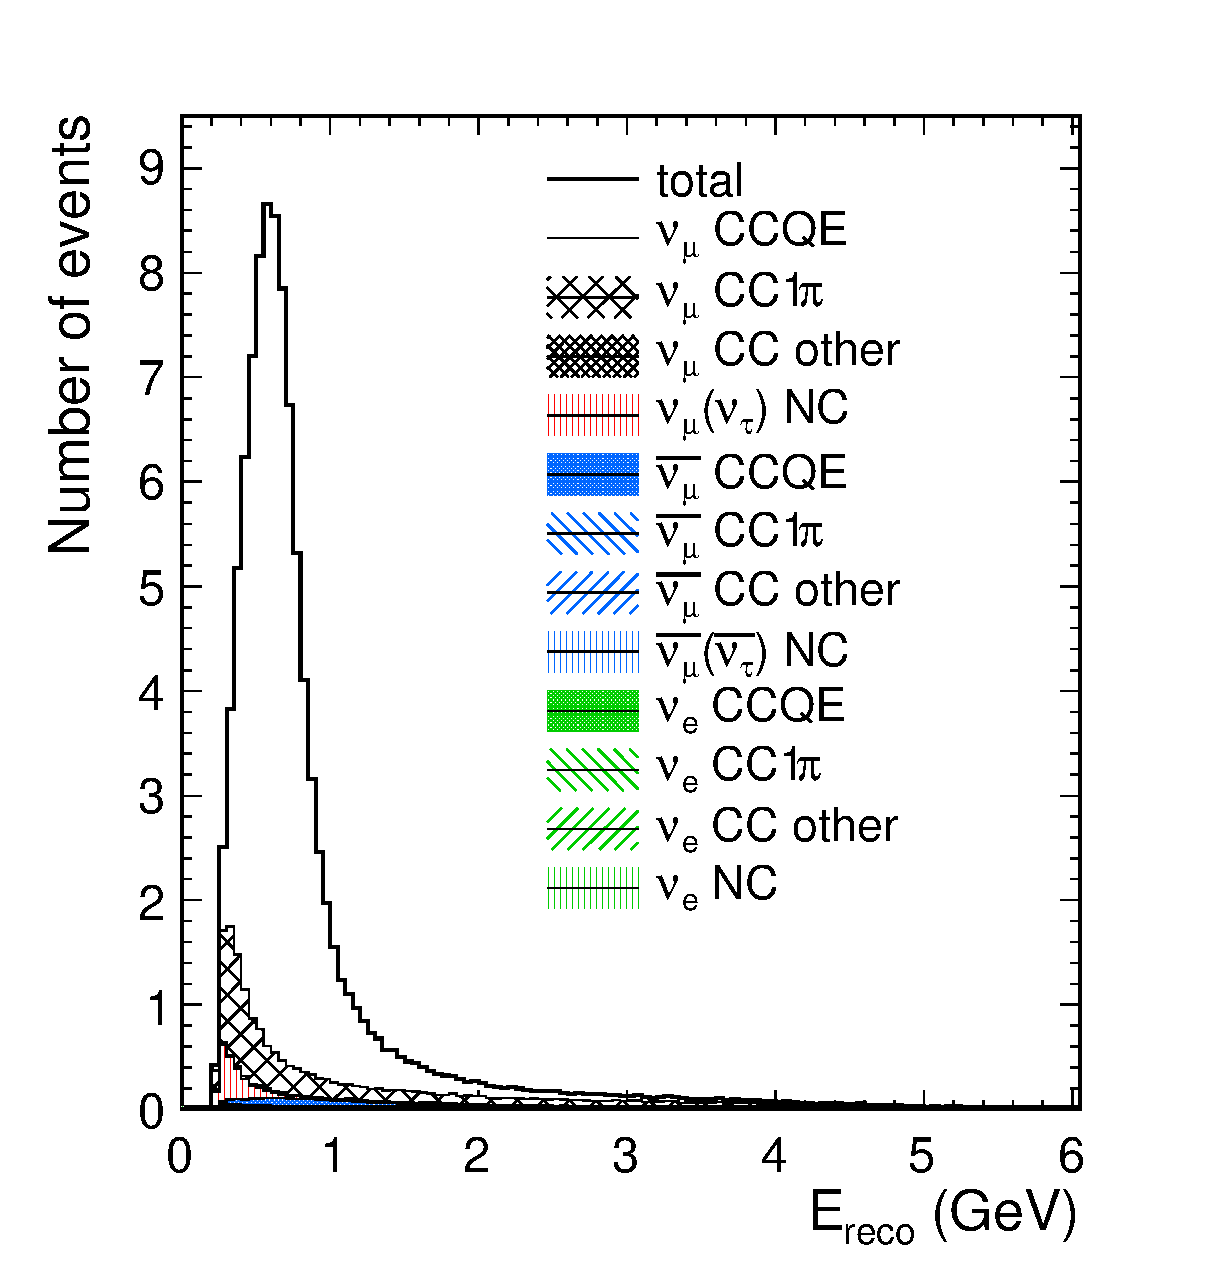
\includegraphics[width=19pc,height=19pc]{./images/predicted_spectrum/nominal/genie_contrib_noosc.eps}
\caption{
  Predicted non-oscillated reconstructed-energy spectrum of 1-ring $\mu$-like events (after extrapolation)
  and contributions from various true neutrino reaction modes (GENIE).
}
\label{fig:genie_mode_contrib_noosc}
\end{minipage}
\hspace{0.04\linewidth}
\begin{minipage}[t]{0.48\linewidth}
\centering
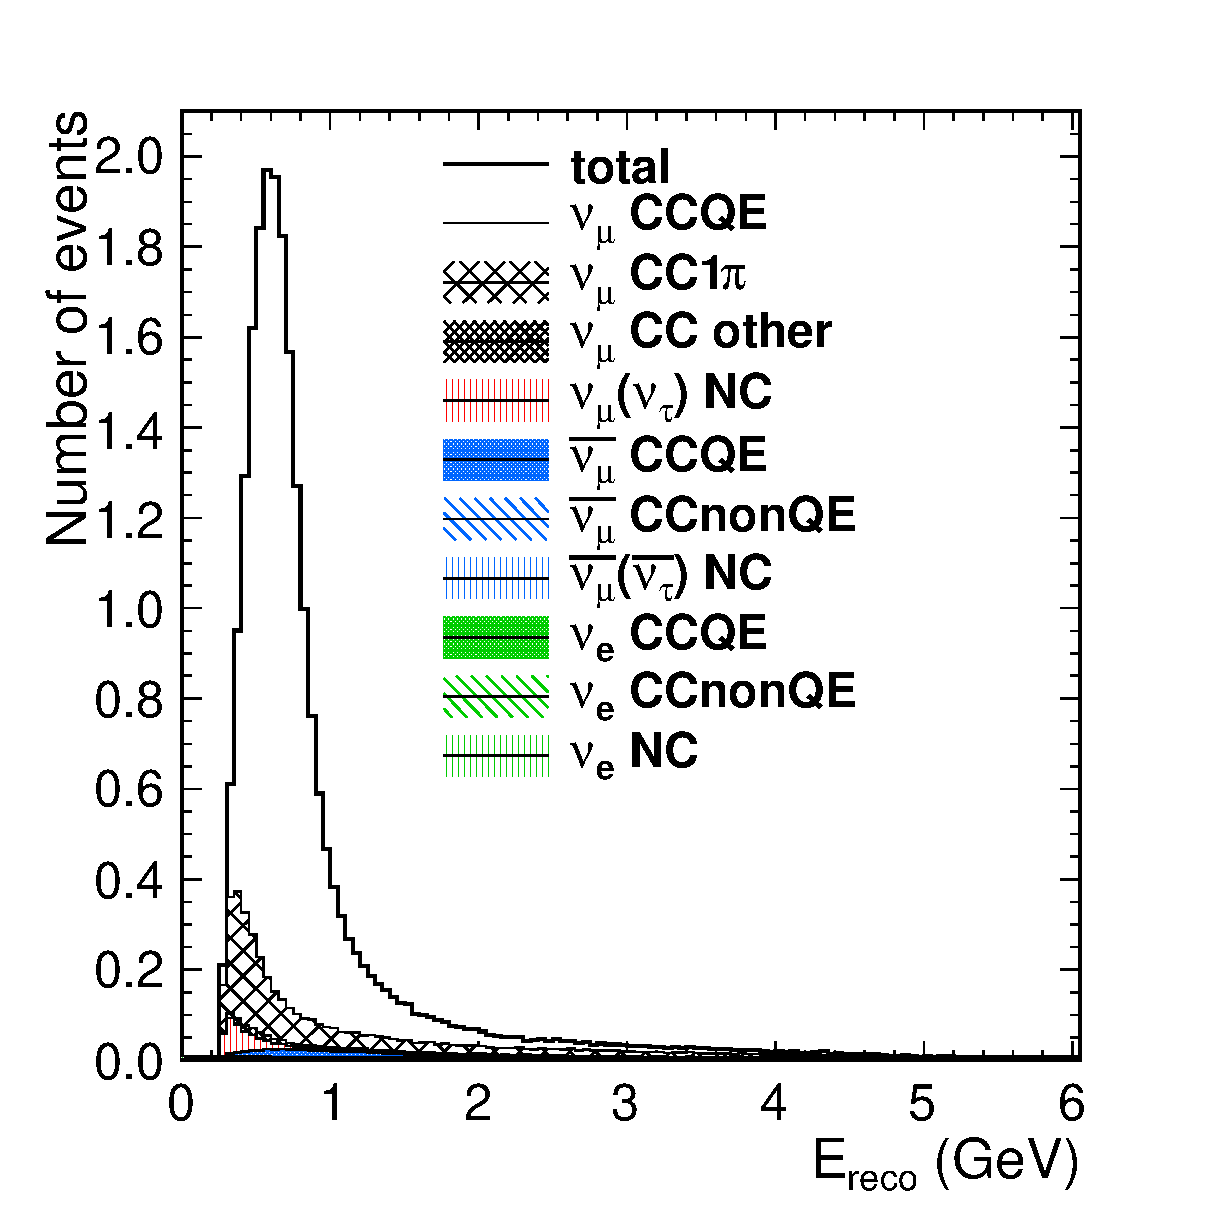
\includegraphics[width=19.5pc,height=19pc]{images/predicted_spectrum/nominal/neut_contrib_noosc.eps}
\caption{
  Predicted non-oscillated reconstructed-energy spectrum of 1-ring $\mu$-like events (after extrapolation)
  and contributions from various true neutrino reaction modes (NEUT).
}
\label{fig:neut_mode_contrib_noosc}
\end{minipage}
\end{figure}


\begin{figure}[ht]
\begin{minipage}[t]{0.48\linewidth}
\centering
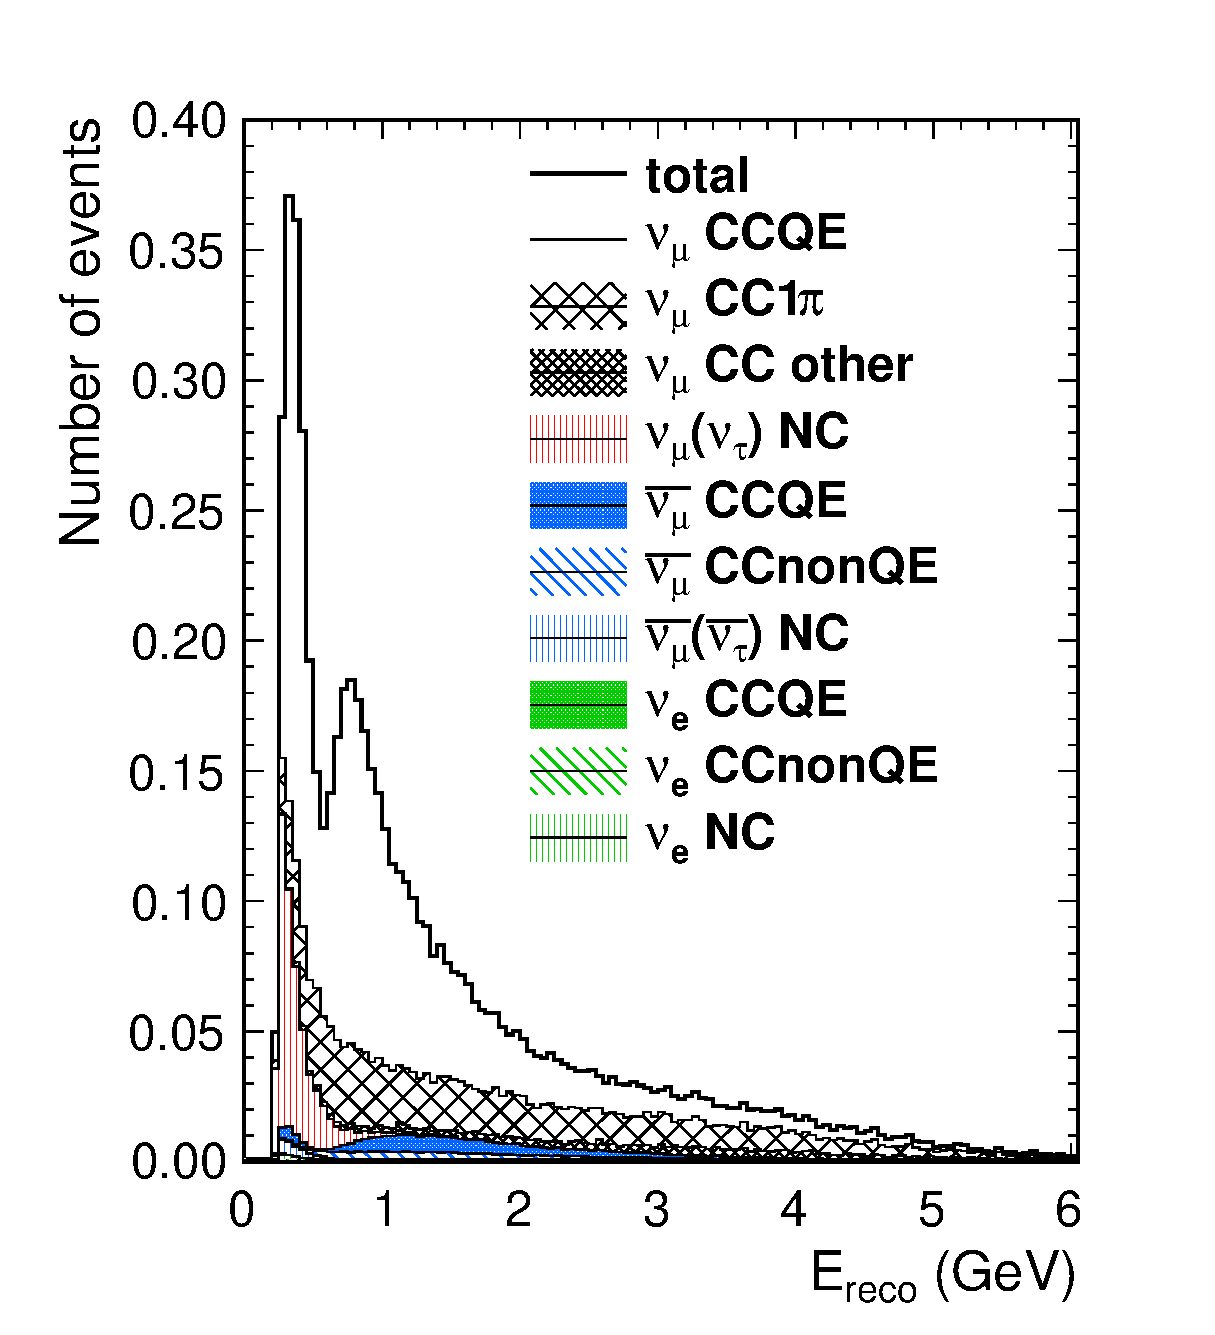
\includegraphics[width=19pc,height=19pc]{./images/predicted_spectrum/nominal/genie_contrib_2p4Em3_1p0.eps}
\caption{
  Predicted oscillated ($sin^{2}2\theta_{23}$ = 1.0 and $\Delta m^{2}_{23}$ = 2.4$\times10^{-3}$ $eV^{2}/c^{4}$) 
  reconstructed-energy spectrum of 1-ring $\mu$-like events (after extrapolation)
  and contributions from various true neutrino reaction modes (GENIE).
}
\label{fig:genie_mode_contrib_2p4Em3_1p0}
\end{minipage}
\hspace{0.04\linewidth}
\begin{minipage}[t]{0.48\linewidth}
\centering
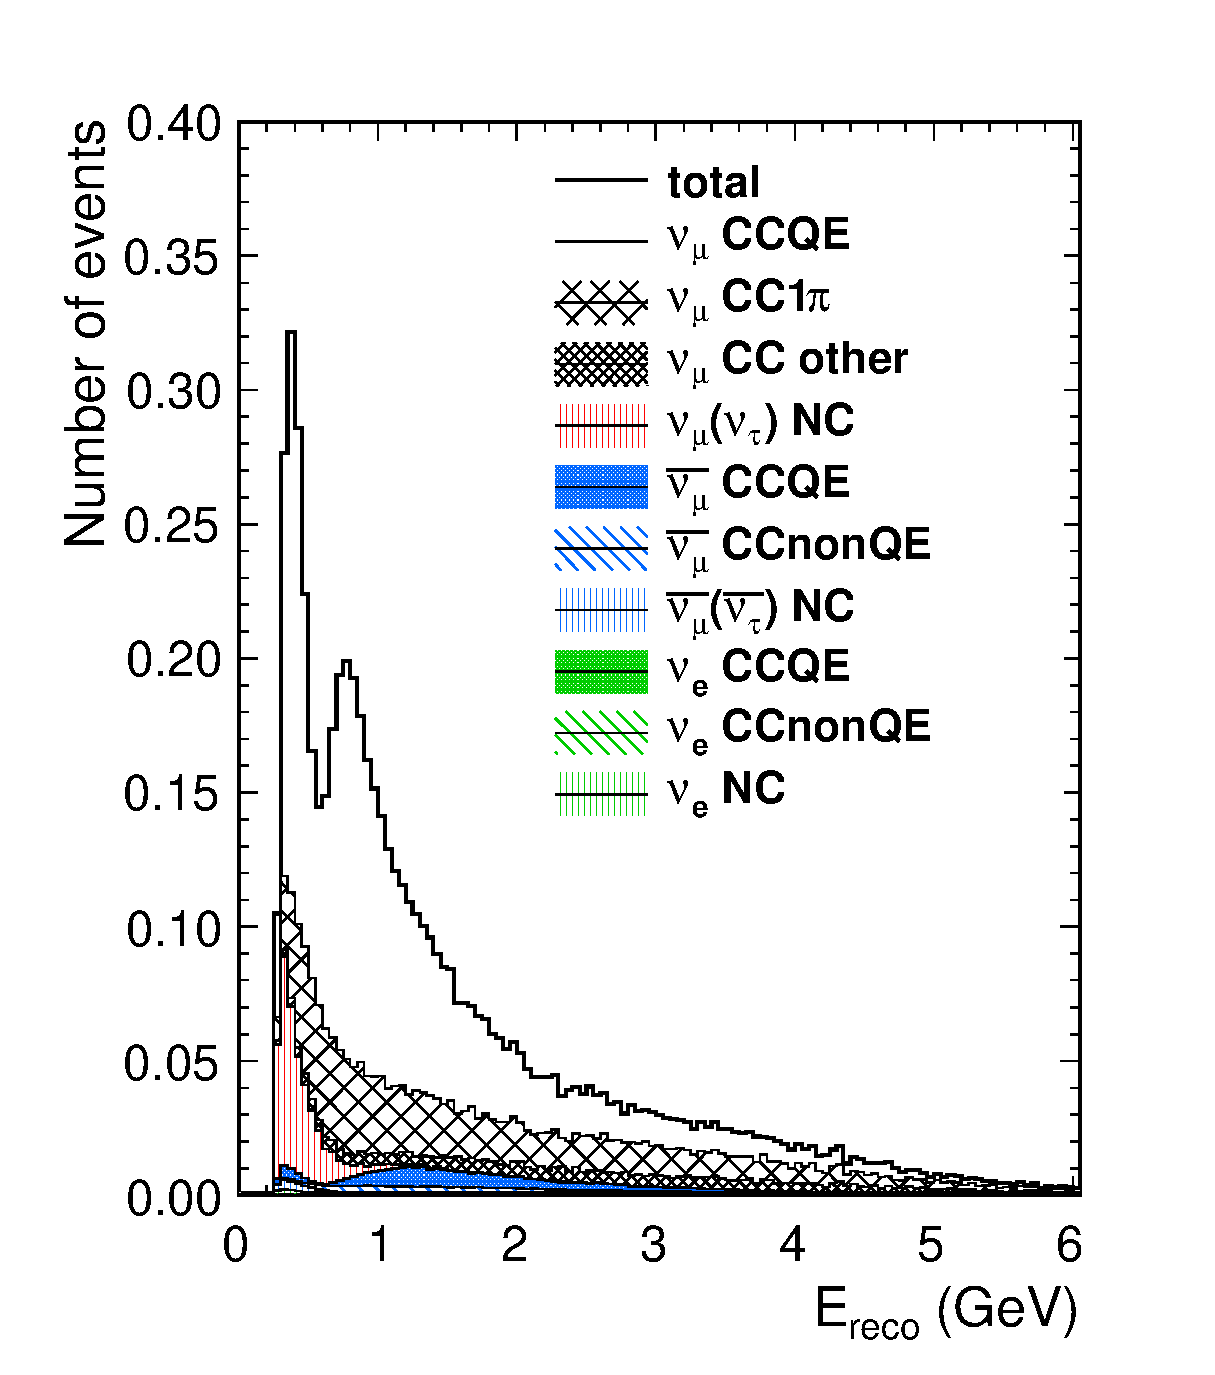
\includegraphics[width=19pc,height=19pc]{images/predicted_spectrum/nominal/neut_contrib_2p4Em3_1p0.eps}
\caption{
  Predicted oscillated ($sin^{2}2\theta_{23}$ = 1.0 and $\Delta m^{2}_{23}$ = 2.4$\times10^{-3}$ $eV^{2}/c^{4}$) 
  reconstructed-energy spectrum of 1-ring $\mu$-like events (after extrapolation)
  and contributions from various true neutrino reaction modes (NEUT).
}
\label{fig:neut_mode_contrib_2p4Em3_1p0}
\end{minipage}
\end{figure}



\begin{table}
\centering
\begin{tabular}{| c || c | c || c | c | }
\hline
   & \multicolumn{2}{c||} { (a) } 
   & \multicolumn{2}{c| } { (b) }\\
                                         & GENIE              & NEUT               & GENIE               & NEUT  \\
\hline
\hline
Total                                    &  22.4193            &  22.8136            &  6.2043             &    6.3395             \\
$\nu_{\mu}$ CCQE                         &  18.0269 (80.408\%) &  18.0707 (79.210\%) &  3.5785 (57.678\%)  &    3.5944 (56.699\%)   \\
$\nu_{\mu}$ CC1$\pi$                     &   2.8527 (12.724\%) &   3.0883 (13.537\%) &  1.4488 (23.352\%)  &    1.5163 (23.918\%)   \\
$\nu_{\mu}$ CCother                      &   0.2995  (1.336\%) &   0.5219 (2.288\%)  &  0.2514  (4.052\%)  &    0.4056 (6.398\%)   \\
$\nu_{\mu}$($\nu_{\tau}$) NC             &   0.4720  (2.106\%) &   0.3767 (1.651\%)  &  0.4720  (7.608\%)  &    0.3767 (5.942\%)   \\
$\bar{\nu_{\mu}}$ CCQE                   &   0.4854  (2.165\%) &   0.5027 (2.203\%)  &  0.2375  (3.828\%)  &    0.2526 (3.985\%)   \\
$\bar{\nu_{\mu}}$ CCnonQE                &   0.2383  (1.063\%) &   0.2160 (0.947\%)  &  0.1716  (2.765\%)  &    0.1564 (2.468\%)   \\
$\bar{\nu_{\mu}}$($\bar{\nu_{\tau}}$) NC &   0.0273  (0.122\%) &   0.0219 (0.096\%)  &  0.0273  (0.440\%)  &    0.0219 (0.345\%)   \\
$\nu_{e}$ CCQE                           &   0.0016  (0.007\%) &   0.0017 (0.008\%)  &  0.0016  (0.026\%)  &    0.0017 (0.027\%)   \\
$\nu_{e}$ CCnonQE                        &   0.0012  (0.005\%) &   0.0015 (0.006\%)  &  0.0012  (0.020\%)  &    0.0015 (0.023\%)   \\
$\nu_{e}$ NC                             &   0.0144  (0.064\%) &   0.0124 (0.054\%)  &  0.0144  (0.232\%)  &    0.0124 (0.195\%)   \\
\hline
\end{tabular}
\caption{
  Expected numbers of SuperK 1-ring $\mu$-like events from GENIE and NEUT (after extrapolation) for 
  (a) no oscillation and 
  (b) oscillations with $sin^{2}2\theta_{23}$ = 1.0 and $\Delta m^{2}_{23}$ = 2.4$\times10^{-3}$ $eV^{2}/c^{4}$.
}
\label{tab:genie_neut_mode_contrib}
\end{table}



\begin{figure}[ht]
\begin{minipage}[t]{0.47\linewidth}
\centering
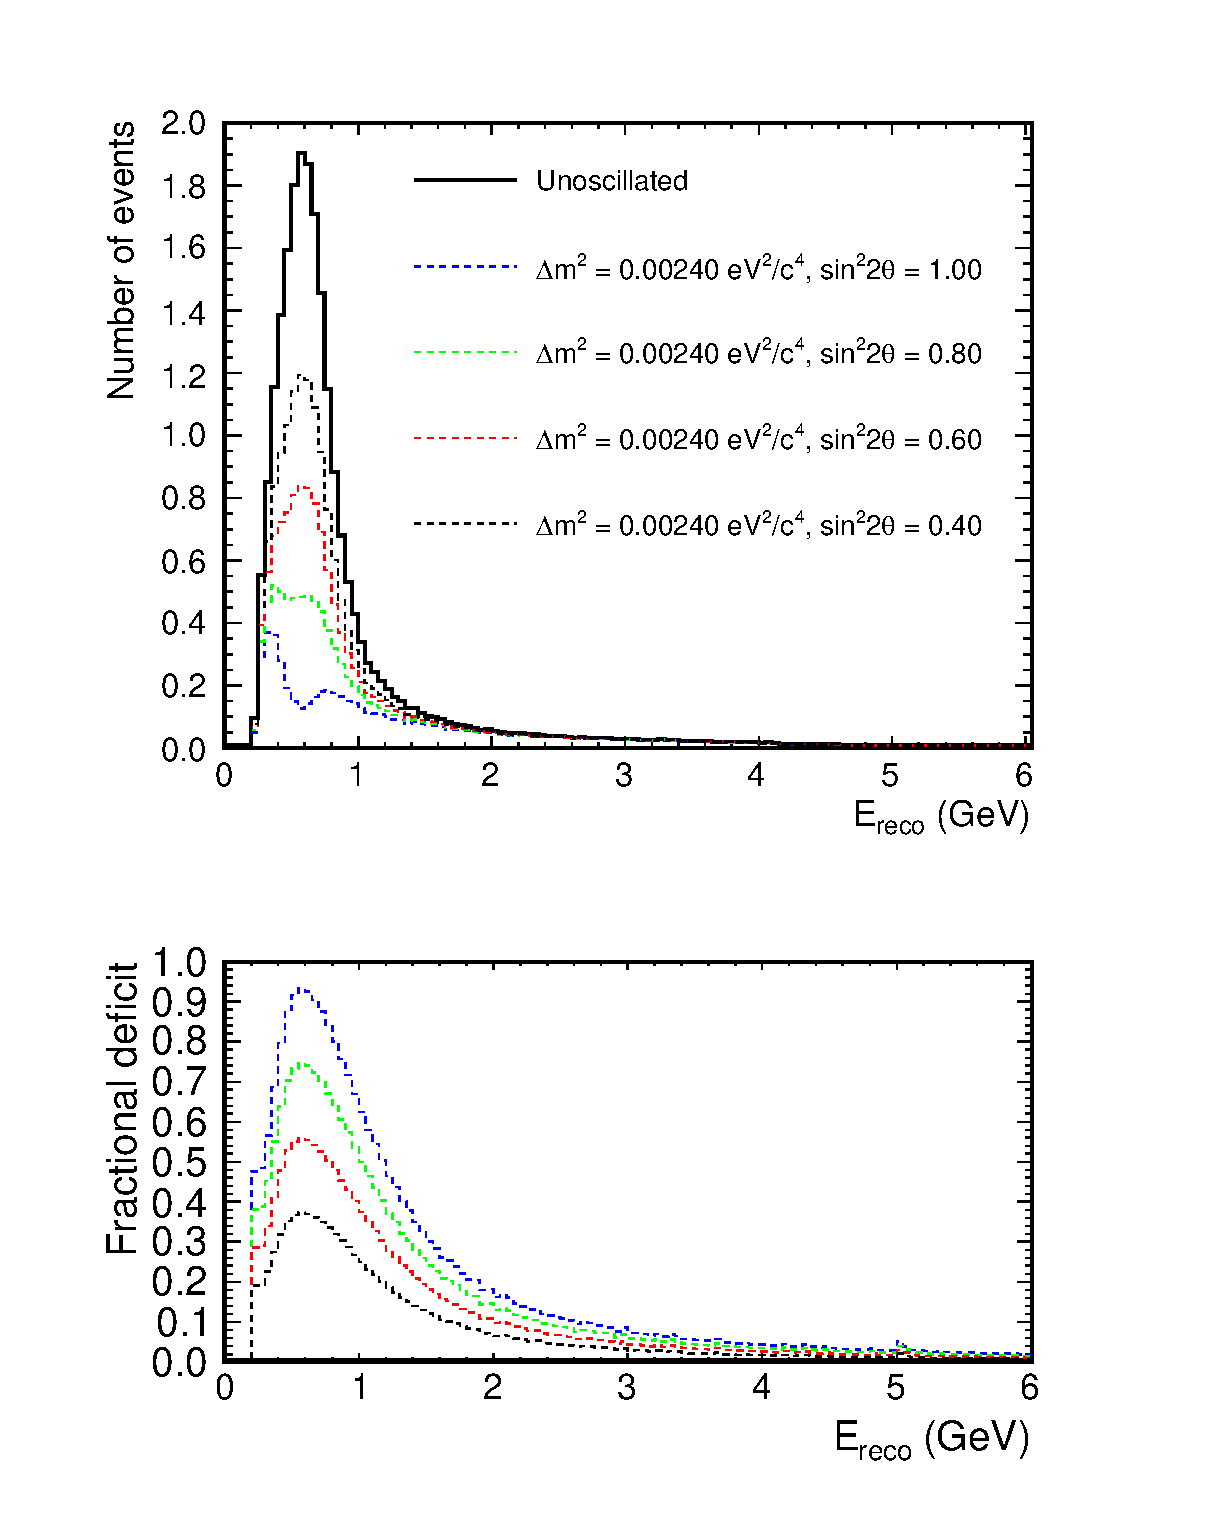
\includegraphics[width=19pc,height=22pc]{./images/predicted_spectrum/nominal/genie_sk_spectrum_2p4Em3_twk_sinsq2theta.eps}
\caption{
  Predicted reconstructed-energy spectrum of 1-ring $\mu$-like events (after extrapolation)
  for $\Delta m^{2}_{23}$ = 2.4$\times10^{-3}$ $eV^{2}/c^{4}$ and
  $sin^{2}2\theta_{23}$ = 1.0, 0.8, 0.6, 0.4. 
  The non-oscillated spectrum is also shown (GENIE).
}
\label{fig:genie_sk_spectrum_twk_sinsq2theta}
\end{minipage}
\hspace{0.06\linewidth}
\begin{minipage}[t]{0.47\linewidth}
\centering
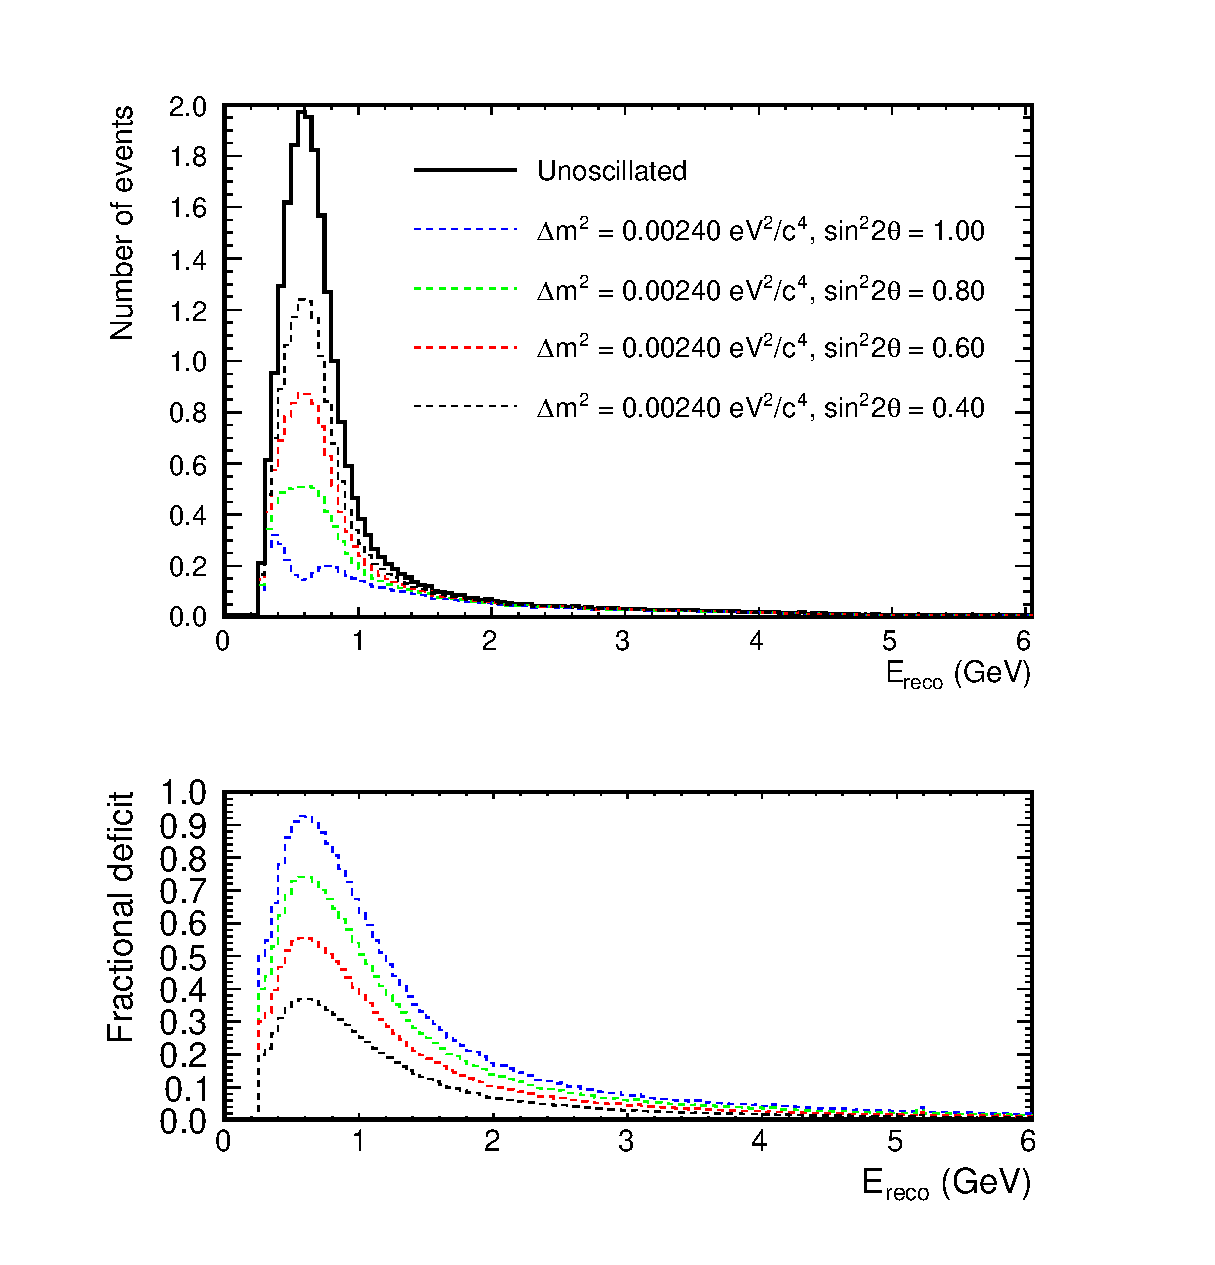
\includegraphics[width=19pc,height=22pc]{images/predicted_spectrum/nominal/neut_sk_spectrum_2p4Em3_twk_sinsq2theta.eps}
\caption{
  Predicted reconstructed-energy spectrum of 1-ring $\mu$-like events (after extrapolation)
  for $\Delta m^{2}_{23}$ = 2.4$\times10^{-3}$ $eV^{2}/c^{4}$ and
  $sin^{2}2\theta_{23}$ = 1.0, 0.8, 0.6, 0.4. 
  The non-oscillated spectrum is also shown (NEUT).
}
\label{fig:neut_sk_spectrum_twk_sinsq2theta}
\end{minipage}
\end{figure}


\begin{table}
\centering
\begin{tabular}{| c | c | c | c | c | c | c | c | c | c | c | }
\hline
$E_{reco}$
   & \multicolumn{2}{c|} { (a) } 
   & \multicolumn{2}{c|} { (b) }
   & \multicolumn{2}{c|} { (c) }
   & \multicolumn{2}{c|} { (d) }
   & \multicolumn{2}{c|} { (e) }\\
           (GeV) & GENIE  & NEUT     & GENIE  & NEUT     & GENIE  & NEUT    & GENIE  & NEUT    & GENIE  & NEUT  \\
\hline
\hline
$<$  0.50        &  7.442 &  6.526   &  1.691 &  1.379   &  2.841 &  2.408  &  3.991 &  3.438  &  5.142 &  4.467 \\
$<$  0.75        & 15.528 & 15.114   &  2.490 &  2.239   &  5.098 &  4.814  &  7.705 &  7.389  & 10.313 &  9.964 \\
$<$  1.00        & 18.392 & 18.315   &  3.252 &  3.065   &  6.280 &  6.115  &  9.308 &  9.165  & 12.336 & 12.215 \\
$<$  1.50        & 20.101 & 20.245   &  4.180 &  4.100   &  7.364 &  7.329  & 10.548 & 10.558  & 13.732 & 13.787 \\
$<$  2.00        & 20.839 & 21.063   &  4.751 &  4.729   &  7.969 &  7.996  & 11.186 & 11.263  & 14.404 & 14.592 \\
$<$  4.00        & 22.068 & 22.417   &  5.864 &  5.956   &  9.105 &  9.248  & 12.346 & 12.540  & 15.586 & 15.833 \\
$<$ 10.00        & 22.419 & 22.814   &  6.204 &  6.340   &  9.447 &  9.634  & 12.690 & 12.929  & 15.933 & 16.224 \\
\hline
\end{tabular}
\caption{
  Expected numbers of SuperK 1-ring $\mu$-like events from GENIE and NEUT (after extrapolation) for
  various reconstructed energy slices and oscillation hypotheses.
  The non-oscillated expectations are shown in (a), while (b)-(e) show the oscillated expectation 
  for $\Delta m^{2}_{23}$ = 2.4$\times10^{-3}$ $eV^{2}/c^{4}$ 
  and various neutrino mixing angles:
  (b) $sin^{2}2\theta_{23}$ = 1.0,
  (c) $sin^{2}2\theta_{23}$ = 0.8, 
  (d) $sin^{2}2\theta_{23}$ = 0.6 and 
  (e) $sin^{2}2\theta_{23}$ = 0.4.
}
\label{tab:genie_neut_nsk_twk_sinsq2theta}
\end{table}



\begin{figure}[ht]
\begin{minipage}[t]{0.47\linewidth}
\centering
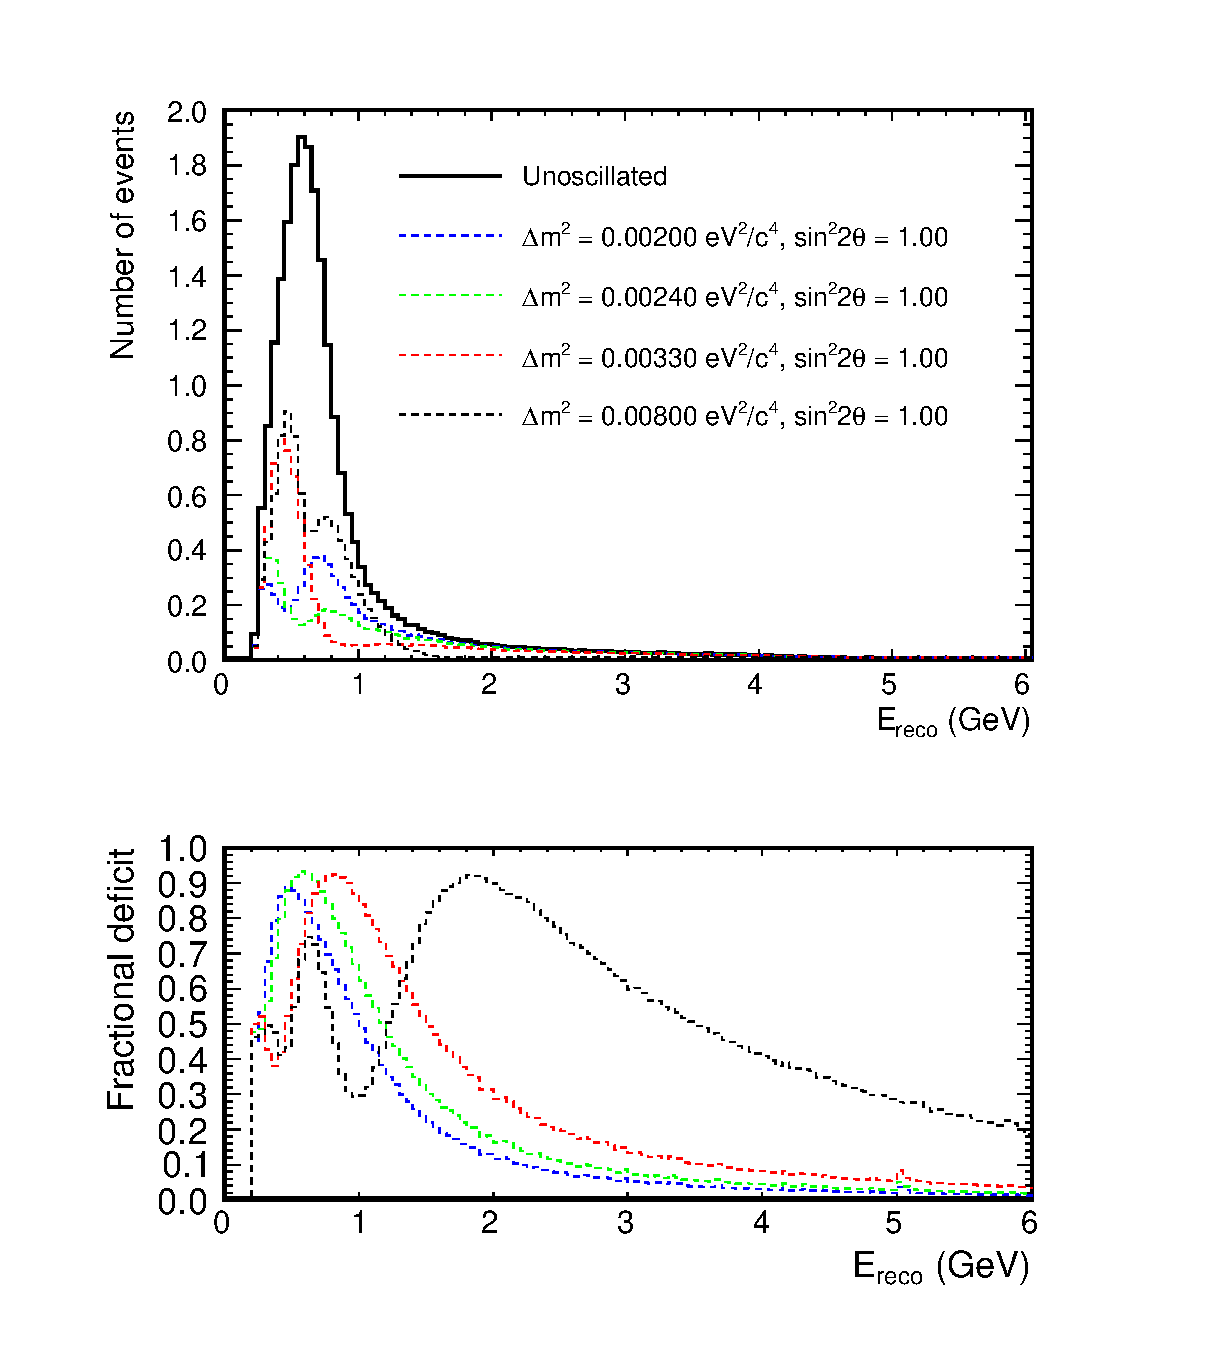
\includegraphics[width=19pc,height=22pc]{./images/predicted_spectrum/nominal/genie_sk_spectrum_1p0_twk_dmsq.eps}
\caption{
  Predicted reconstructed-energy spectrum of 1-ring $\mu$-like events (after extrapolation)
  for $sin^{2}2\theta_{23}$ = 1.0 and  
  $\Delta m^{2}_{23}$ =
    2.0$\times10^{-3}$ $eV^{2}/c^{4}$,
    2.4$\times10^{-3}$ $eV^{2}/c^{4}$,
    3.3$\times10^{-3}$ $eV^{2}/c^{4}$ and
    8.0$\times10^{-3}$ $eV^{2}/c^{4}$.
  The non-oscillated spectrum is also shown (GENIE).
}
\label{fig:genie_sk_spectrum_twk_dmsq}
\end{minipage}
\hspace{0.06\linewidth}
\begin{minipage}[t]{0.47\linewidth}
\centering
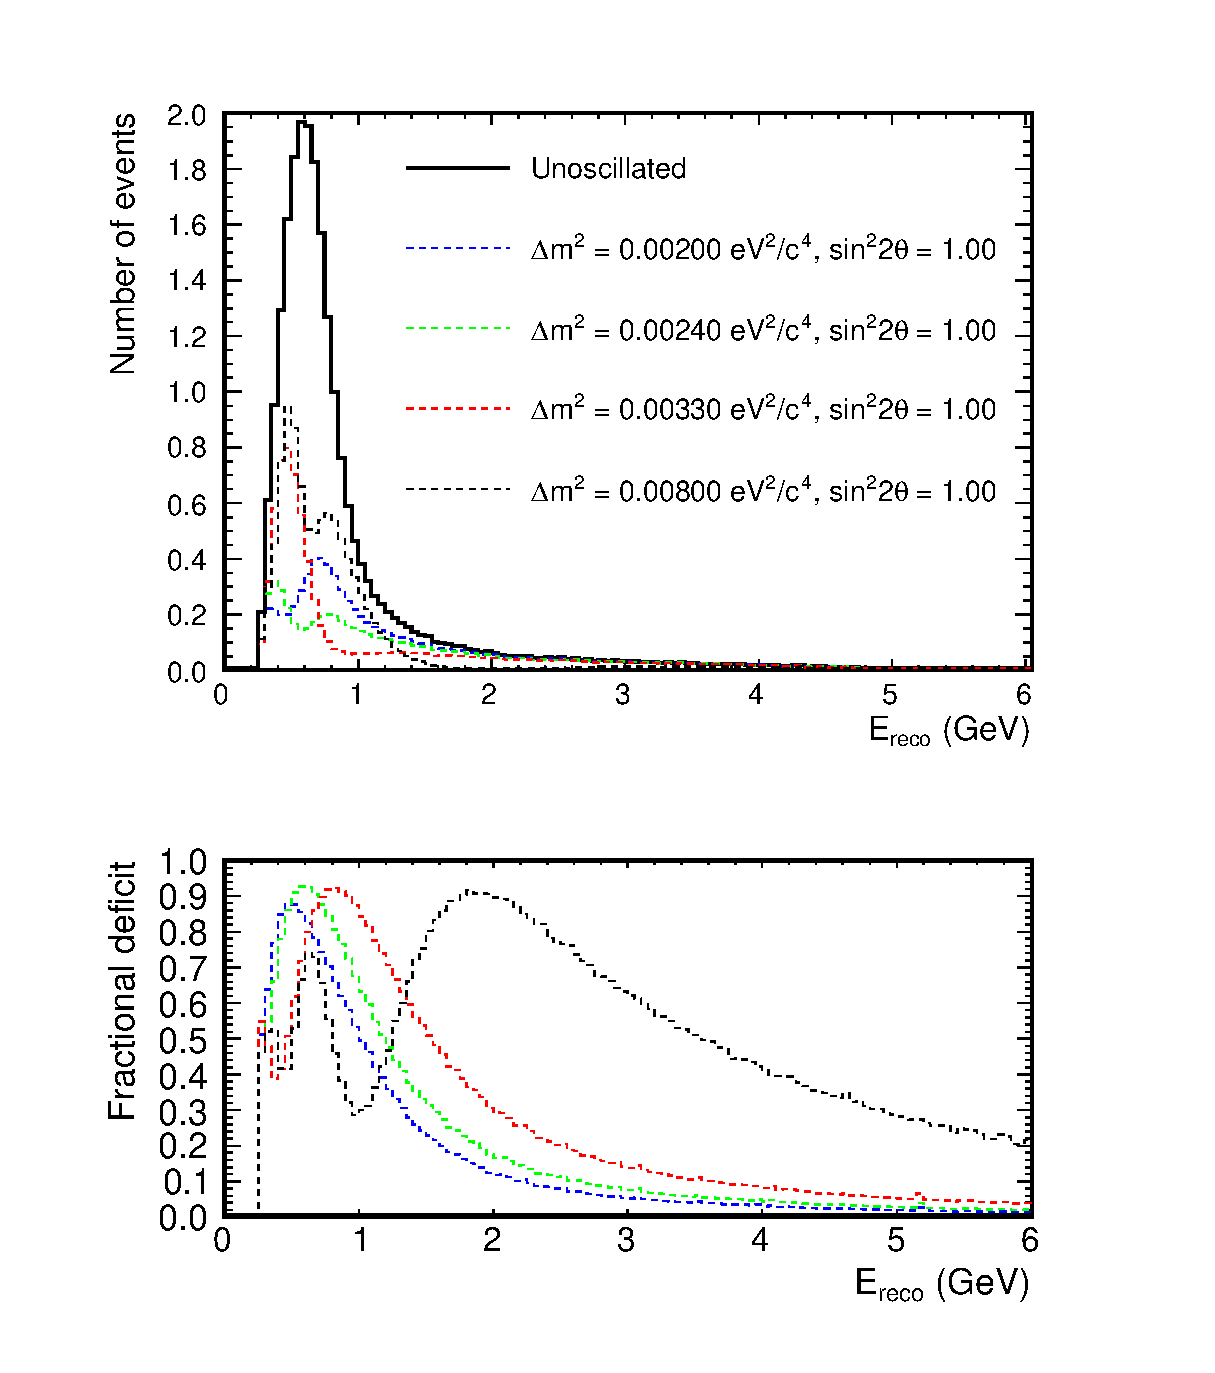
\includegraphics[width=19pc,height=22pc]{images/predicted_spectrum/nominal/neut_sk_spectrum_1p0_twk_dmsq.eps}
\caption{
  Predicted reconstructed-energy spectrum of 1-ring $\mu$-like events (after extrapolation)
  for $sin^{2}2\theta_{23}$ = 1.0 and  
  $\Delta m^{2}_{23}$=
    2.0$\times10^{-3}$ $eV^{2}/c^{4}$,
    2.4$\times10^{-3}$ $eV^{2}/c^{4}$,
    3.3$\times10^{-3}$ $eV^{2}/c^{4}$ and
    8.0$\times10^{-3}$ $eV^{2}/c^{4}$.
  The non-oscillated spectrum is also shown (NEUT).
}
\label{fig:neut_sk_spectrum_twk_dmsq}
\end{minipage}
\end{figure}



\begin{table}
\centering
\begin{tabular}{| c | c | c | c | c | c | c | c | c | c | c | }
\hline
$E_{reco}$
   & \multicolumn{2}{c|} { (a) } 
   & \multicolumn{2}{c|} { (b) }
   & \multicolumn{2}{c|} { (c) }
   & \multicolumn{2}{c|} { (d) }
   & \multicolumn{2}{c|} { (e) }\\
           (GeV) & GENIE  & NEUT     & GENIE  & NEUT     & GENIE  & NEUT    & GENIE  & NEUT    & GENIE  & NEUT  \\
\hline
\hline
$<$  0.50        &  7.442 &  6.526   &  1.416 &  1.170   &  1.691 &  1.379  &  3.752 &  3.252  &  3.919 &  3.245 \\
$<$  0.75        & 15.528 & 15.114   &  3.128 &  2.977   &  2.490 &  2.239  &  5.070 &  4.718  &  6.501 &  6.189 \\
$<$  1.00        & 18.392 & 18.315   &  4.303 &  4.264   &  3.252 &  3.065  &  5.357 &  5.038  &  8.336 &  8.203 \\
$<$  1.50        & 20.101 & 20.245   &  5.421 &  5.516   &  4.180 &  4.100  &  5.909 &  5.647  &  9.136 &  9.139 \\
$<$  2.00        & 20.839 & 21.063   &  6.039 &  6.198   &  4.751 &  4.729  &  6.364 &  6.145  &  9.213 &  9.231 \\
$<$  4.00        & 22.068 & 22.417   &  7.186 &  7.462   &  5.864 &  5.956  &  7.385 &  7.269  &  9.623 &  9.672 \\
$<$ 10.00        & 22.419 & 22.814   &  7.529 &  7.850   &  6.204 &  6.340  &  7.716 &  7.641  &  9.868 &  9.947 \\
\hline
\end{tabular}
\caption{
  Expected numbers of SuperK 1-ring $\mu$-like events from GENIE and NEUT (after extrapolation) for
  various reconstructed energy slices and oscillation hypotheses.
  The non-oscillated expectations are shown in (a), while (b)-(e) show the oscillated expectation 
  for $sin^{2}2\theta_{23}$ = 1.0
  and squared neutrino mass differences:
  (b) $\Delta m^{2}_{23}$ = 2.0$\times10^{-3}$ $eV^{2}/c^{4}$,
  (c) $\Delta m^{2}_{23}$ = 2.4$\times10^{-3}$ $eV^{2}/c^{4}$,
  (d) $\Delta m^{2}_{23}$ = 3.3$\times10^{-3}$ $eV^{2}/c^{4}$ and
  (e) $\Delta m^{2}_{23}$ = 8.0$\times10^{-3}$ $eV^{2}/c^{4}$
}
\label{tab:genie_neut_nsk_twk_dmsq}
\end{table}


\begin{figure}[ht]
\begin{minipage}[t]{0.47\linewidth}
\centering
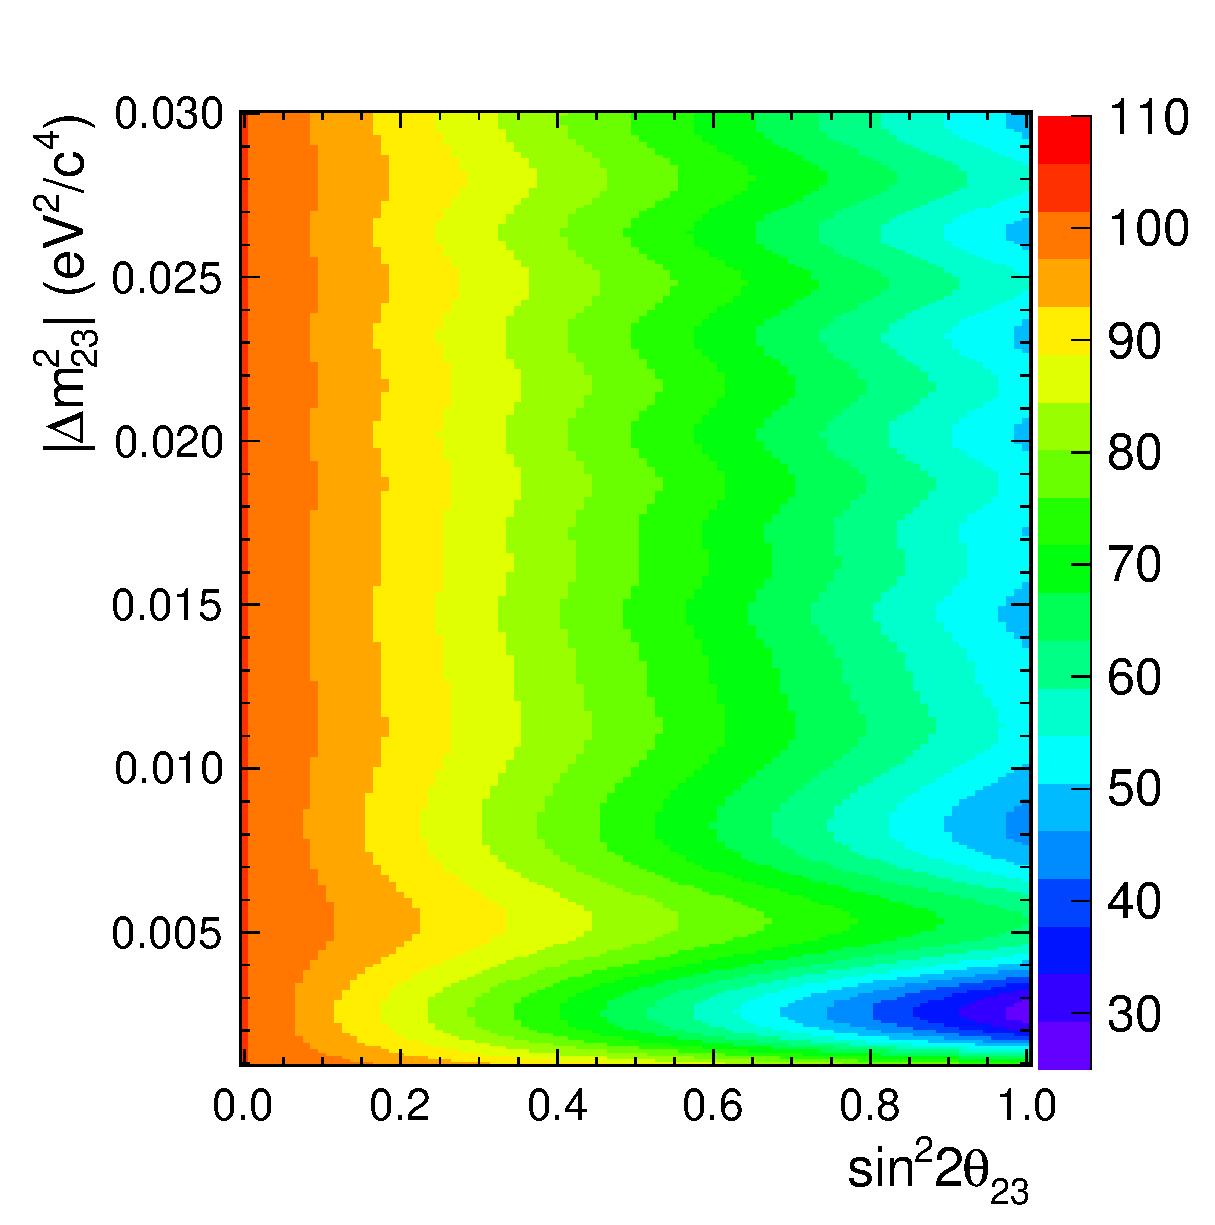
\includegraphics[width=18pc,height=16pc]{./images/predicted_spectrum/nominal/genie_nsk_osc.eps}
\caption{
  Expected number of 1-ring $\mu$-like events (after extrapolation) in the 0-10 GeV reconstructed 
  energy range (GENIE).
}
\label{fig:genie_nsk_osc_param_grid}
\end{minipage}
\hspace{0.06\linewidth}
\begin{minipage}[t]{0.47\linewidth}
\centering
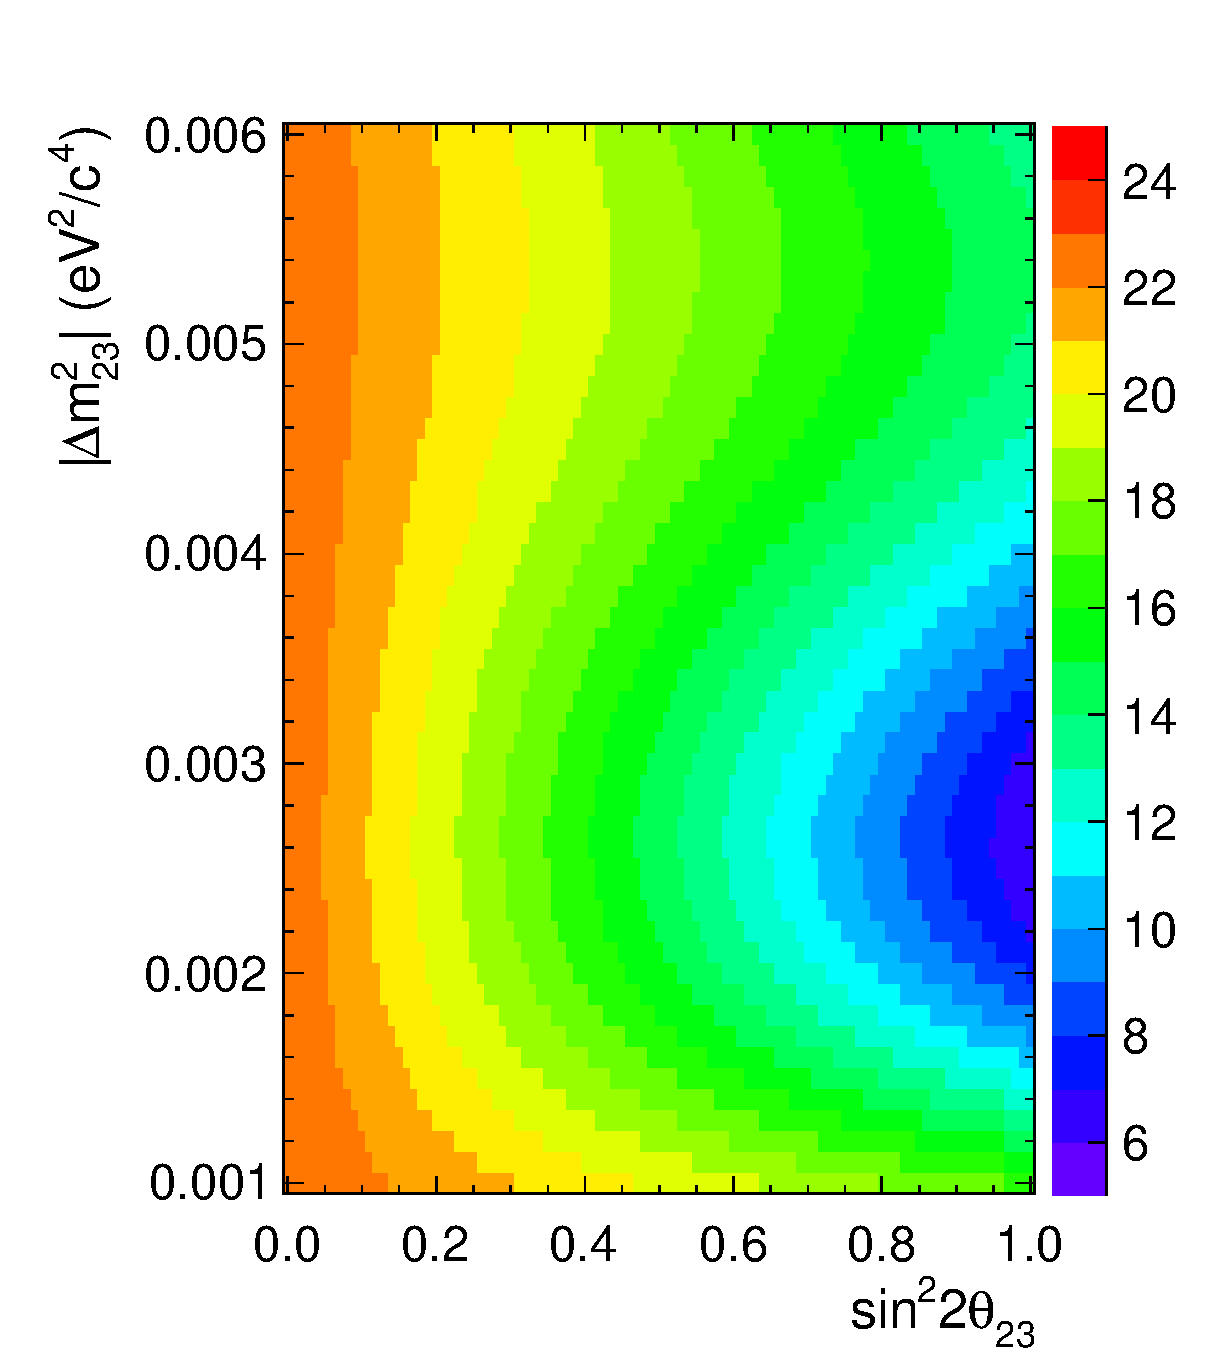
\includegraphics[width=17pc,height=16pc]{images/predicted_spectrum/nominal/neut_nsk_osc.eps}
\caption{
  Expected number of 1-ring $\mu$-like events (after extrapolation) in the 0-10 GeV reconstructed 
  energy range (NEUT).
}
\label{fig:neut_nsk_osc_param_grid}
\end{minipage}
\end{figure}


\begin{figure*}[htb]
\center
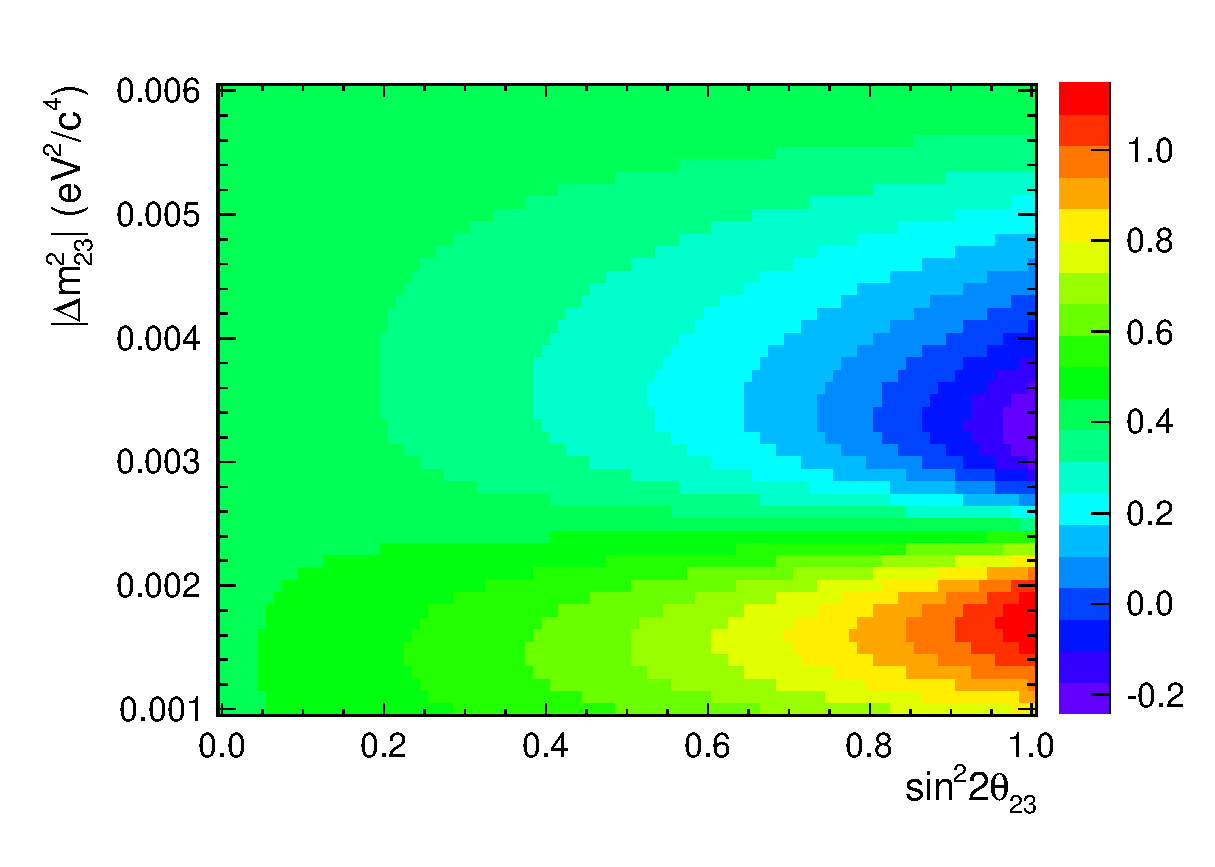
\includegraphics[width=38pc]{./images/predicted_spectrum/nominal/genie_neut_nsk_diff_osc.eps}
\caption{
  Percentage difference $100\cdot(N^{NEUT}_{SK}-N^{GENIE}_{SK})/(N^{NEUT}_{SK}+N^{GENIE}_{SK})/2$ 
  between the GENIE and NEUT
  expected numbers of 1-ring $\mu$-like events (after extrapolation) 
  in the 0-10 GeV reconstructed energy range. 
  The percentage difference in the -0.2\% to +1.2\% range
  (Compare with Fig. \ref{fig:nsk_uncertainty_osc_param_grid_xsec_err_only}).
}
\label{fig:genie_neut_nsk_difference_osc_param_grid}
\end{figure*}

\clearpage

\section {Oscillation fitting method} 
\label{sec:fitting}

\subsection {Outline}

Measurements of the oscillation parameters $sin^{2}2\theta_{23}$, $\Delta m^{2}_{23}$
are obtained by comparing the observed and predicted SuperK reconstructed energy spectra
for 1-ring $\mu$-like events.
Let $N$ be the number of reconstructed energy bins and
${\bf a}$ be a $1 \times N_{s}$ - dimensional array of systematic (nuisance) 
parameters that affect the SuperK reconstructed energy spectrum prediction (e.g
parameters that control the beam and neutrino interaction simulations and 
the detector response).
Best-fit values are obtained by minimizing: 
\begin{equation}
\displaystyle
\chi^{2} (sin^{2}2\theta_{23},\Delta m^{2}_{23}; {\bf a}) = 
  2 \cdot \sum_{i=0}^{N-1} 
   \Big( 
     n^{obs}_{i} \cdot ln(n^{obs}_{i}/n^{exp}_{i}) +
     (n^{exp}_{i}-n^{obs}_{i}) 
   \Big) +
   ({\bf a}-{\bf a_{0}})^{T} \cdot {\bf C}^{-1} \cdot ({\bf a}-{\bf a_{0}})
\label{eq:chisquare}
\end{equation}
where
${\bf a_{0}}$ is an $1 \times N_{s}$ - dimensional array with the default values of 
considered systematics parameters, ${\bf a}^{T}$ is the transpose of ${\bf a}$,
${\bf C}$ is the systematic parameter covariance matrix of dimension $N_{s} \times N_{s}$,
$n^{obs}_{i}$ is the observed number of events in the $i^{th}$ bin, and
$n^{exp}_{i} = n^{exp}_{i}(sin^{2}2\theta_{23},\Delta m^{2}_{23}; {\bf a})$ 
is the corresponding expected number of events.

Due to the limited statistics in SuperK 
and the limited amount of information available to this analysis from the near detectors,
we do not fit for systematics.  Instead, we evaluate oscillation systematics as described
in section \ref{sec:eval_osc_systematics}.



%
%
% Likelihood function & 
% Comparison of K2K/MINOS fit methods
%
%

\subsection {Construction of the likelihood function and comparison of the `MINOS' and `K2K' methods }
\label{sec:K2K_MINOS_fit_comparison}

In this analys, we use a fitting method previously employed by MINOS \cite{MinosDisappearanceAnalysis}.
The construction of the likelihood function is described in this section in detail.
We use a likelihood ratio method, 
whereas J.Kameda's analysis uses a
%%\footnote
%%{ 
%%  Input p.d.f's come from Monte Carlo samples that have an intrinsic 50 MeV energy binning 
%%  (binning of the flux histograms used during event generation).
%%}
maximum likelihood
method previously employed by K2K \cite{K2KDisappearanceAnalysis}.
These two methods give identical results for the best-fit oscillation parameters (for same input p.d.f's).

Let ${\bf n^{obs}}$ be a set of $N$ measurements (the number of events in each of the $N$ bins
\footnote
{
  In this analysis we use 200 50-MeV bins in the 0-10 GeV reconstructed neutrino energy range.
}
).
The probability density function (p.d.f.) for the total number of events 
$n^{obs}_{tot} = \sum_{i=0}^{N-1} n^{obs}_{i}$
observed in SuperK has a 
Poisson distribution, and the mean of that distribution is equal to the predicted total number 
of events $n^{exp}_{tot} = n^{exp}_{tot}(sin^{2}2\theta_{23},\Delta m^{2}_{23}; {\bf a})
= \sum_{i=0}^{N-1} n^{exp}_{i}(sin^{2}2\theta_{23},\Delta m^{2}_{23}; {\bf a})$. 
The p.d.f. is
\begin{equation}
\begin{array}{rcl}
\displaystyle
f_{poisson} = 
f_{poisson}({\bf n^{obs}}; sin^{2}2\theta_{23},\Delta m^{2}_{23}; {\bf a}) = 
   \frac{\left[n^{exp}_{tot}\right]^{n^{obs}_{tot}}
   e^{-n^{exp}_{tot}}}{n^{obs}_{tot}!} 
\end{array}
\label{eq:pdf_poisson}
\end{equation}

The reconstructed energies of the observed events are distributed over $N$ bins. 
Since there are $N$ possible outcomes for the process of placing an event in a bin, 
the p.d.f.\ of the distribution of those outcomes is multinomial:
\begin{equation}
\begin{array}{rcl}
\displaystyle
f_{multinomial} = 
f_{multinomial}({\bf n^{obs}}; sin^{2}2\theta_{23},\Delta m^{2}_{23}; {\bf a}) = 
   n^{obs}_{tot}!\prod_{i=0}^{N-1} 
   \frac{1}{n^{obs}_{i}!} 
   P_{i}^{n^{obs}_{i}} 
\end{array}
\label{eq:pdf_multinomial_1}
\end{equation}
where $P_{i} = P_{i}(sin^{2}2\theta_{23},\Delta m^{2}_{23}; {\bf a})$
is the probability that an event is placed in the $i^{th}$ bin. 
This probability can be calculated as the ratio of the 
number of events predicted for that bin to the predicted total number of events:
\begin{equation}
\displaystyle
  P_{i} = 
  \frac{n^{exp}_{i}(sin^{2}2\theta_{23},\Delta m^{2}_{23}; {\bf a})}
       {n^{exp}_{tot}(sin^{2}2\theta_{23},\Delta m^{2}_{23}; {\bf a})}
\label{eq:prob_in_multinomial}
\end{equation}
Therefore, $f_{multinomial}$ can be written as
\begin{equation}
\begin{array}{rcl}
\displaystyle
f_{multinomial} = 
   n^{obs}_{tot}!\prod_{i=0}^{N-1} \frac{1}{n^{obs}_{i}!} 
   \left[\frac{n^{exp}_{i}}
              {n^{exp}_{tot}} \right]^{n^{obs}_{i}} 
\end{array}
\label{eq:pdf_multinomial_2}
\end{equation}

The joint p.d.f.\ $f_{joint} = f({\bf n^{obs}}; sin^{2}2\theta_{23},\Delta m^{2}_{23}; {\bf a})$ 
for the outcome of the reconstructed energy distribution 
is the product of the Poisson and multinomial distributions
shown in Eq.\ \ref{eq:pdf_poisson} and Eq.\ \ref{eq:pdf_multinomial_2} 
respectively:
\begin{equation}
\displaystyle
f_{joint} = 
   e^{-n^{exp}_{tot}} 
   \prod_{i=0}^{N-1} \frac{1}{n^{obs}_{i}!} 
   \left[n^{exp}_{i}\right]^{n^{obs}_{i}} 
\label{eq:reco_hist_pdf}
\end{equation}
 
In our analysis, we use the p.d.f.\ in Eq.\ \ref{eq:reco_hist_pdf}, and this is identical to the likelihood function used 
by K2K in \cite{K2KDisappearanceAnalysis}: 
L$_{NORM}$ corresponds to the Poisson term and L$_{SHAPE}$ to the multinomial term. 
However there is also a difference between the two analyses. K2K used the ``maximum likelihood'' method, i.e.\ the best-fit 
values of the oscillation parameters were obtained by taking the natural 
logarithm of Eq.\ \ref{eq:reco_hist_pdf}, and maximising it with respect to those parameters. We use the ``likelihood ratio''
method, which involves dividing the p.d.f. in Eq.\ \ref{eq:reco_hist_pdf} by a factor that does not depend on the oscillation parameters.
The best-fit values of the oscillation parameters are unchanged by such a division (see \cite{StatAnalysisCowan} for 
further details). 

In our analysis, the p.d.f.\ in Eq.\ \ref{eq:reco_hist_pdf} is divided by

\begin{equation}
\displaystyle
f_{0} = f_{0}({\bf n^{obs}}) = 
  \frac{\left[n^{obs}_{tot}\right]^{n^{obs}_{tot}}e^{-n^{obs}_{tot}}}{n^{obs}_{tot}!} n^{obs}_{tot}! 
       \prod_{i=0}^{N-1} \frac{1}{n^{obs}_{i}!} \left[\frac{n^{obs}_{i}}{n^{obs}_{tot}} \right]^{n^{obs}_{i}}
\label{eq:division_factor}
\end{equation}
Cancelling the factors of $n^{obs}_{tot}!$ and using $n^{obs}_{tot} = \sum_{i=0}^{N-1}n^{obs}_{i}$, Eq.\ \ref{eq:division_factor} simplifies to
\begin{equation}
\displaystyle
f_{0} = 
  e^{-n^{obs}_{tot}}  
  \prod_{i=0}^{N-1} 
  \frac{1}{n^{obs}_{i}!} \left[n^{obs}_{i} \right]^{n^{obs}_{i}}
\label{eq:division_factor_simple}
\end{equation}
Dividing Eq. \ref{eq:reco_hist_pdf} by Eq. \ref{eq:division_factor_simple} gives the likelihood ratio $\lambda$:
\begin{equation}
\displaystyle
\lambda = e^{n^{obs}_{tot}-n^{exp}_{tot}} 
   \prod_{i=0}^{N-1} \left(\frac{n^{exp}_{i}}{n^{obs}_{i}} \right)^{n^{obs}_{i}}
\label{eq:lambda}
\end{equation}
In the large-sample limit, the quantity
\begin{equation}
\displaystyle
-2 \, \textrm{ln} \lambda = 
   2 \sum_{i=0}^{N-1} 
   \left[n^{obs}_{i} \: \textrm{ln} \left(\frac{n^{obs}_{i}}{n^{exp}_{i}} \right) + 
   n^{exp}_{i} - n^{obs}_{i} \right]
\label{eq:minusloglambda}
\end{equation}
has a $\chi^{2}$ distribution. Best-fit values of the oscillation parameters 
are obtained by varying their values in the input to
$n^{exp}_{i}$ until the minimum of -2ln$\lambda$ is found. 
The reader should compare Eq. \ref{eq:minusloglambda} with the statistical
term of Eq. \ref{eq:chisquare} shown in previous section.


\subsection {Oscillation parameter range}
\label{sec:osc_par_limits}

The search for the minimum value of 
$\chi^{2} (sin^{2}2\theta_{23},\Delta m^{2}_{23}; {\bf a})$ (see Eq. \ref{eq:chisquare}) 
is performed in the range 
$0 \leq$ $sin^{2}2\theta_{23}$ $\leq 1$ and
$1 \times 10^{-3} eV^{2}/c^{4} \leq$ $|\Delta m^{2}_{23}|$ $\leq 6 \times 10^{-3} eV^{2}/c^{4}$.
Values of $sin^{2}2\theta_{23}$ $> 1$  are not permitted; although it is numerically allowed and,
occasionally, it yields better fits to data, it has no physical interpretation within the context
in which we attempt to interpret the data (2-flavour neutrino oscillations) and causes p.d.f's to 
have pathological behaviour.
The maximum allowed value of $|\Delta m^{2}_{23}|$ is $6 \times 10^{-3} eV^{2}/c^{4}$.
Due to the sinusoidal nature of the oscillation survival probability function,
statistical fluctuations in the present small-statistics dataset can, very rarely, 
cause a global minimum in large $|\Delta m^{2}_{23}|$ ($> 6 \times 10^{-3} eV^{2}/c^{4}$). 
As a $|\Delta m^{2}_{23}|$ of $6 \times 10^{-3} eV^{2}/c^{4})$ is already more than 10 $\sigma$
away from the MINOS central value we, a priori, prevent $\chi^{2} (sin^{2}2\theta_{23},\Delta m^{2}_{23}; {\bf a})$ 
minima in the wrong trough of the survival probability function.

%
%
% Calculation of confidence contours
%
%

\subsection {Calculation of confidence contours}
\label{sec:contours}

In this work we have used two different methods for calculating confidence regions:
(1) The PDG recommendation on quoting uncertainties on parameters measured jointly (see Sec. \ref{sec:contour_pdg}) and 
(2) The Feldman-Cousins method (see Sec. \ref{sec:contour_fc}).
The PDG method is used for illustration purposes only because of its simplicity.
Due to concerns regarding confidence region coverage, 
the Feldman-Cousins method is used for all physics results.
Both methods are discussed briefly.

\subsubsection {Method 1: PDG recommendation}
\label{sec:contour_pdg}

The PDG recommendation on quoting uncertainties on parameters measured jointly
($sin^{2}2\theta_{23}$, $\Delta m^{2}_{23}$ in our analysis) is described in \cite{RevPartPhys}.
It is a fully frequentist treatment using the Gaussian approximation.
One finds the best-fit point and calculates the confidence contours as lines of constant $\Delta{\chi^{2}}$
from this point. Therefore, a confidence region is defined by:
\begin{equation}
\displaystyle
\chi^{2}(sin^{2}2\theta_{23},\Delta m^{2}_{23}) < \chi_{min}^{2} + \Delta{\chi^{2}}
\label{eq:chiconfregion}
\end{equation}
Values of $\Delta{\chi^{2}}$ for obtaining confidence regions of given statistical significance
are given in Tab. \ref{table:deltachi2table} for 1, 2 and 3 simultaneously-determined parameters.
In future discussions we will be referring to the confidence regions obtained using this method as 
`plain'.

\begin{table*}[htb]
\center
\renewcommand{\arraystretch}{1.75} % enlarge line spacing
\begin{tabular}{|cc|cccc|}
\hline
                  &    & \multicolumn {4}{|c|} { {\bf Confidence level} } \\
                  &    & {\bf 68\%}      & {\bf 90\%}     &  {\bf 95\%}   &   {\bf 99\%} \\
\hline
\multirow{3}{*}{ \begin{sideways} {\bf $N_{params}$} \end{sideways}}
  &   ${\bf 1}$ & 1.00          & 2.71           &  3.84         &   6.63       \\
  &   ${\bf 2}$ & 2.30          & 4.61           &  5.99         &   9.21       \\
  &   ${\bf 3}$ & 3.53          & 6.25           &  7.82         &   11.34      \\
\hline
\end{tabular}\\[2pt]
\caption{
Values of $\Delta{\chi^{2}}$ used for calculating confidence regions in the $\nu_{\mu}$-disappearance 
parameter space, for a given confidence level and a given number of fit parameters.
}
\label{table:deltachi2table}
\end{table*}

\subsubsection {Method 2: The Feldman-Cousins method}
\label{sec:contour_fc}

The work of Feldman and Cousins \cite{FeldmanCousins} 
uses the freedom which is inherent in the Neyman construction of confidence regions, 
to address cases 
(in particular, cases with
Poisson processes with background and Gaussian errors near a physical boundary)
where classical construction of confidence regions produces overcoverage, undercoverage, or
in extreme cases, an empty region.
Using the Feldman-Cousins method, construction of the confidence region proceeds as follows:

The sin$^{2}$2$\theta_{23}$ - $\Delta$m$^{2}_{23}$ plane is divided into a square grid of size 
sin$^{2}$2$\theta_{23}$ = 0.01, $\Delta$m$^{2}_{23}$ = 0.1 $\times$ 10$^{-3}$ $eV^{2}/c^{4}$. 
Grid points are taken to be the values of sin$^{2}$2$\theta_{23}$ and $\Delta$m$^{2}_{23}$ 
at the centre of each grid square. 
For each grid point, sets of toy MC experiments were generated
with the oscillation parameters of that grid point. 
Typically, 10000 toy MC experiments were made for each grid point including systematic variations, 
and 3000 datasets were made for each grid point without these systematic variations.

The best-fit values of the oscillation parameters are found for each MC experiment 
by minimising -2 ln$\lambda$ in Eq. \ref{eq:minusloglambda}.
It must be emphasised that, for the Feldman-Cousins method, 
the best-fit values are restricted to the physical region (sin$^{2}$2$\theta_{23}$ $<$ 1). 
Using these best-fit parameters, the value of $\Delta\chi^{2}_{MC}$ is calculated as follows:
\begin{equation}
\displaystyle
\Delta \chi^{2}_{MC} = \chi^{2} \textrm{(true)} - \chi^{2} \textrm{(MC, best fit)}
\label{eq:deltachi2}
\end{equation}
where $\chi^{2}$ is as defined in Eq. \ref{eq:chisquare}, 
``true'' means the true values of the oscillation parameters at that grid point, and 
``best fit'' means the best-fit values for that MC experiment. 
The quantity $\Delta \chi^{2}_{MC}$ in Eq. \ref{eq:deltachi2} is equivalent 
to that given in Eq. 5.6 in \cite{FeldmanCousins}; 
it is always $>=$0 since the best fit is at the minimum value of $\chi^{2}$. 

For each grid point, the critical value of $\Delta\chi^{2}$ ($\Delta\chi^{2}_{CRIT}$) 
is found such that $\alpha$ of the fake experiments have $\Delta\chi^{2}_{MC}$ $<$ $\Delta\chi^{2}_{CRIT}$, 
where $\alpha$ is the desired confidence level. 
The principal difference between the Feldman-Cousins and PDG methods is that the former determines 
the value of $\Delta\chi^{2}_{CRIT}$ individually for each grid point, whereas the latter uses the same value 
for all grid points (see Tab. \ref{table:deltachi2table}). 
It is possible to draw a Feldman-Cousins $\Delta\chi^{2}_{CRIT}$ 
surface in the sin$^{2}$(2$\theta_{23}$ - $\Delta$m$^{2}_{23}$ plane, 
and examples of such surfaces are shown in Fig. \ref{fig:fc_delta_chisq}. 
From this figure, it can be seen that grid points near the physical boundary of 
sin$^{2}$(2$\theta_{23}$ = 1 have lower values of $\Delta\chi^{2}_{CRIT}$ than points in the middle of the grid; 
this is due to the requirement that best-fit points be within the physical region. 
In an unconstrained fit, some best-fit points would lie outside the physical region; 
requiring them to be in the physical region causes them to pile up at the physical boundary, 
where they have lower values of $\Delta\chi^{2}_{MC}$ than they would have in an unconstrained fit.

Using the T2K 2010a data, Feldman-Cousins confidence contours are drawn such that grid points 
with $\Delta\chi^{2}_{DATA}$ $<$ $\Delta\chi^{2}_{CRIT}$ are included within the contour, 
where $\Delta\chi^{2}_{DATA}$ is given by
\begin{equation}
\displaystyle
\Delta \chi^{2}_{DATA} = \chi^{2} \textrm{(true)} - \chi^{2} \textrm{(data, best fit)}
\label{qe:fccontour}
\end{equation} 


\begin{figure*}[htb]
\center
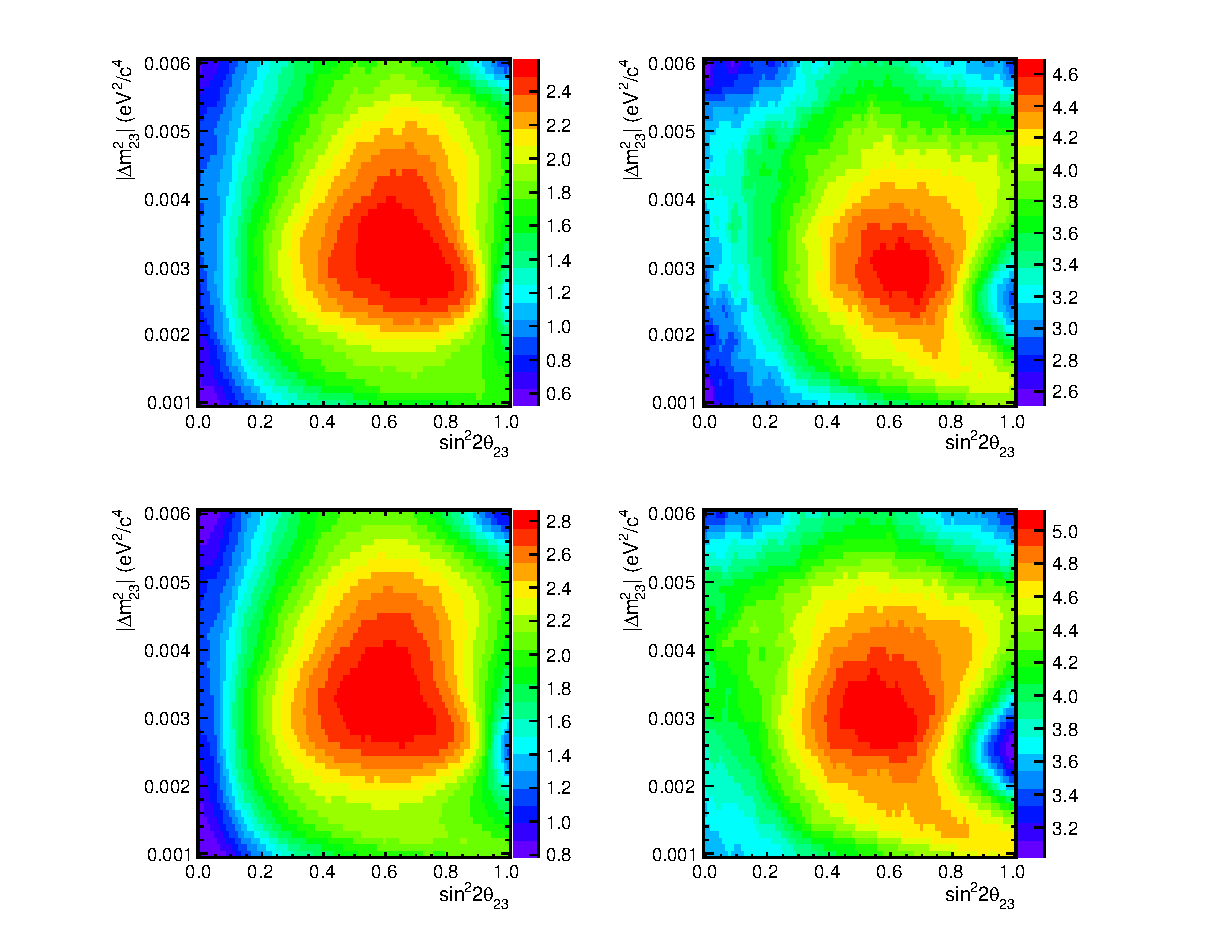
\includegraphics[width=38pc]{./images/fits/feldman_cousins/fc_delta_chisq.eps}
\caption{
  Monte Carlo estimation, 
  according to the Feldman-Cousins method,
  of $\Delta\chi^{2}_{68}$ (left) and $\Delta\chi^{2}_{90}$ (right)
  as functions of $sin^{2}{2\theta_{23}}$ and $\Delta{m^{2}_{23}}$,
  for calculation of the 68\% CL and 90\% CL, respectively, confidence regions
  for the $3.23 \times 10^{19}$-POT T2K $\nu_{\mu}$-disappearance analysis.
  The top row shows $\Delta\chi^{2}$ surfaces calculated using statistical errors
  only whereas the bottom row shows $\Delta\chi^{2}$ surfaces calculated using 
  both statistical and systematic erros.
  We observe that values of $\Delta\chi^{2}$ decrease as one moves closer to the 
  physical boundaries at $sin^{2}{2\theta_{23}}$ = 0 and $sin^{2}{2\theta_{23}}$ = 1 
  and the fit (`search'/`sensitivity') $\Delta{m^{2}_{23}}$ boundaries.
}
\label{fig:fc_delta_chisq}
\end{figure*}

\begin{figure*}[htb]
\center
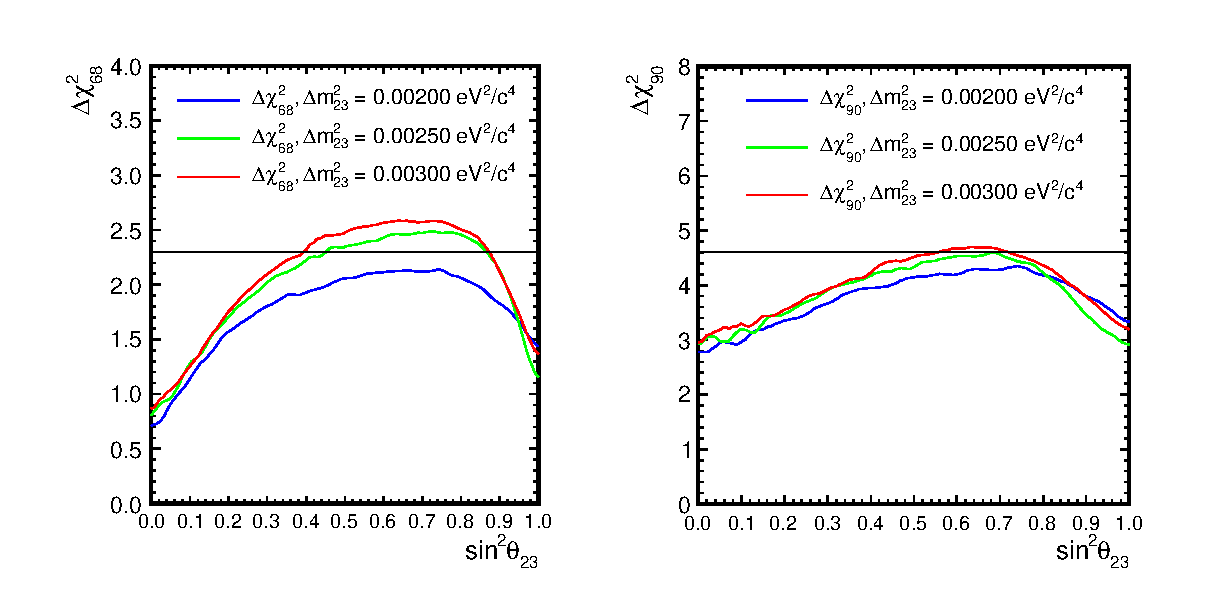
\includegraphics[width=38pc]{./images/fits/feldman_cousins/fc_delta_chisq_stat_vs_sinsq_3dmsq.eps}
\caption{
  Monte Carlo estimation,
  according to the Feldman-Cousins method (statistical errors only),
  of $\Delta\chi^{2}_{68}$ (left) and $\Delta\chi^{2}_{90}$ (right),
  as functions of $sin^{2}{2\theta_{23}}$ for 3 different values of $\Delta{m^{2}_{23}}$ 
  ($2.0 \times 10^{-3} eV^{2}/c^{4}$, 
   $2.5 \times 10^{-3} eV^{2}/c^{4}$ and
   $3.0 \times 10^{-3} eV^{2}/c^{4}$).
  For comparison, the canonical value of $\Delta\chi^{2}$ used in the PDG 
  (see Tab. \ref{table:deltachi2table}) is also shown as a horizontal line.
}
\label{fig:fc_delta_chisq_stat_vs_sinsq_3dmsq}
\end{figure*}

\begin{figure*}[htb]
\center
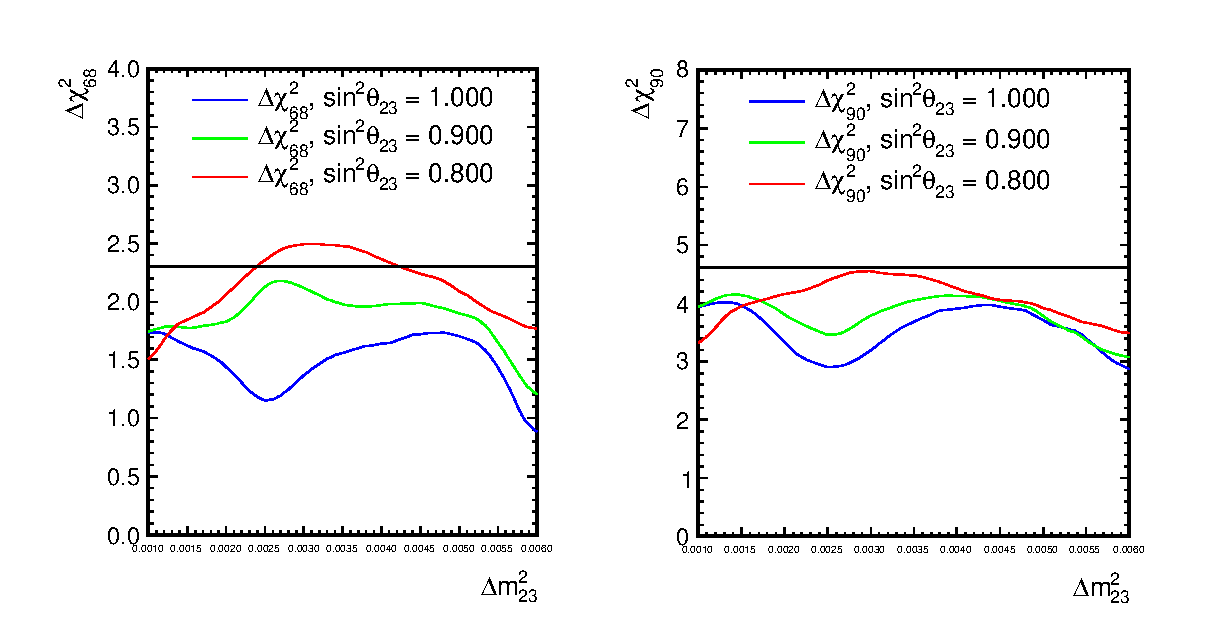
\includegraphics[width=38pc]{./images/fits/feldman_cousins/fc_delta_chisq_stat_vs_dmsq_3sinsq.eps}
\caption{
  Monte Carlo estimation,
  according to the Feldman-Cousins method (statistical errors only),
  of $\Delta\chi^{2}_{68}$ (left) and $\Delta\chi^{2}_{90}$ (right),
  as functions of $\Delta{m^{2}_{23}}$ for 3 different values of $sin^{2}{2\theta_{23}}$ 
  (0.8, 0.9 and 1.0).
  For comparison, the canonical value of $\Delta\chi^{2}$ used in the PDG 
  (see Tab. \ref{table:deltachi2table}) is also shown as a horizontal line.
}
\label{fig:fc_delta_chisq_stat_vs_sinsq_3dmsq}
\end{figure*}



\section {Oscillation systematics}
\label{sec:eval_osc_systematics}


\subsection {Inputs uncertainties for systematic error evaluation}
\label{sec:systematics_inputs}

The uncertainties considered in this analysis are summarized in Tab. \ref{tab:input_uncertainties}.
In the presence of these systematic uncertainties, Eq. \ref{eq:far_prediction_no_nd280_spectrum_final}
may be re-written as
{
\arraycolsep=2pt
\begin{equation}
\displaystyle
\begin{array}{lcl}
  N_{SK;r}^{exp} & = &
    f_{norm} \cdot f_{FSI;r} \cdot (1+\Delta{N_{SK;r}}(f_{E}^{SK})) 
      \frac{ \displaystyle N^{obs}_{ND280;CC-like} }
           { \displaystyle f_{\epsilon}^{ND280} \sum_{m\prime} N^{MC}_{ND280;m\prime} \cdot 
                \displaystyle \Big( \prod_{m_{s}} f_{R_{\sigma};m_{s}} \delta_{m\prime;m_{s}} \Big) }
    \cdot \\
    & &
    {\displaystyle
    \sum_{m,t}
        P_{m;t}^{surv} \cdot
        N_{SK;m;r;t}^{MC} \cdot
        \Big( \prod_{m_{s}} f_{R_{\sigma};m_{s}} \delta_{m;m_{s}} \Big) \cdot
        \Big( f_{\sigma_{CCQE};t} \delta_{m;CCQE} \Big) \cdot
        w^{Ch.}_{m;t}({\bf \rho^{\Phi_{SK}}})
     }
\end{array}
\label{eq:far_prediction_no_nd280_spectrum_final_with_systematics}
\end{equation}
}
As explained in Tab. \ref{tab:input_uncertainties},
the energy scale uncertainty is taken into account by scaling the reconstructed energy distribution
bin edges and, assuming uniform distribution of events within the 50 MeV bins,
calculating the number of events gained from / lost to neighbouring bins.
The term $\Delta{N_{SK;r}}$ in above equation expresses the net gain of events at the 
reconstructed energy bin $r$ as a result of SuperK energy scale variations. 
The term $f_{R_{\sigma};m_{s}}$,
where the index $m_{s}$ runs over CC1$\pi$, CCoth and NC,
denotes the MC template modification factor due to the uncertainty
on any of the cross section ratios (relative to CCQE) described in Tab. \ref{tab:input_uncertainties},
while the term $\delta_{m\prime;m}$ is 1 for $m\prime=m$ and 0 otherwise.
Finally, $w^{Ch.}_{m;t}({\bf \rho^{\Phi_{SK}}})$ denotes flux weights generated from 
the SuperK $\nu_{\mu}$ flux true energy bin-to-bin correlation matrix ${\bf \rho^{\Phi_{SK}}}$
using the Cholesky method (see Sec. \ref{sec:cholesky}). 
These weights (ratios of tweaked over nominal 2010d(v2) $\nu_{\mu}$ neutrino fluxes)
are applied only to the $\nu_{\mu}$ SuperK MC templates
and depend on the true energy bin t. 
The weights are constructed so that they have no effect on the 
integrated number of SuperK 1-ring $\mu$-like events.
All other factors appearing in Eq. \ref{eq:far_prediction_no_nd280_spectrum_final_with_systematics} 
are explained in Tab. \ref{tab:input_uncertainties}.

%
% Table with systematic parameters
%

\begin{table*}[htb]
\center
\renewcommand{\arraystretch}{1.75} % enlarge line spacing
\begin{tabular}{p{0.12\textwidth}p{0.88\textwidth}}
%
% SuperK
%
\hline
\multicolumn {2}{l} { {\bf SuperK detector uncertainties} } \\
\hline
\parbox{0.12\textwidth}
{
   $f_{\epsilon}^{SK}$  
}&
\parbox{0.88\textwidth}
{
    \vspace{0.2cm}
    Combined efficiency uncertainty due to fiducial volume, reduction chain, 
    Outer Detector cut, ring counting and PID cut uncertainties.
    (CCQE: 7.8\%, CCnonQE: 25.5\%, NC: 115.1\%, $\nu_{e}$ CC: 100\% \cite{SuperKAnalysisInputs}).
    Applied to corresponding SuperK MC templates.\\
}\\
\parbox{0.12\textwidth}
{
   $f_{E}^{SK}$  
}&
\parbox{0.88\textwidth}
{
    \vspace{0.2cm}
    Reconstructed energy scale error (1\% \cite{SuperKAnalysisInputs}). 
    Applied to SuperK MC templates by scaling bin edges and,
    assuming uniform distribution of events within the 50 MeV bins, calculating the number of events 
    gained from / lost to neighbouring bins.\\
}\\
\hline
%
% nd280 detector systematics
%
\multicolumn {2}{l} { {\bf ND280 detector uncertainties} } \\
\hline
\parbox{0.12\textwidth}
{ 
   $f_{\epsilon}^{ND280}$  
}&
\parbox{0.88\textwidth}
{
    \vspace{0.2cm}
    Efficiency error (5\% \cite{ND280AnalysisInputs}).
    Applied to ND280 MC templates.\\
}\\
\hline
%
% Beam systematics
%
\multicolumn {2}{l} { {\bf Flux uncertainties} } \\
\hline
\parbox{0.12\textwidth}
{ 
   $f_{norm}$ 
}&
\parbox{0.88\textwidth}
{
    \vspace{0.2cm}
    Flux normalization uncertainty.
    Uncertainty, expressed relatively to the $N_{SK}/N_{ND280}$ ratio predicted by the MC,
    is calculated against oscillation and other systematic parameters 
    using code provided by the Beam WG \cite{BeamNormErrCode}.
    Calculated uncertainty for nominal MC and oscillations with parameters
    $sin^{2}2\theta_{23}$ = 1.00 and $\Delta m^{2}_{23}$ = 2.4$\times10^{-3}$ $eV^{2}/c^{4}$
    is around 6.6\%.\\
}\\
\hline
\parbox{0.12\textwidth}
{ 
    ${\bf \rho^{\Phi_{SK}}}$ 
}&
\parbox{0.88\textwidth}
{
    \vspace{0.2cm}
    Flux shape uncertainty. Expressed in terms of true energy bin-to-bin 
    correlation matrix for SuperK $\nu_{\mu}$ flux provided by the Beam WG \cite{BeamShapeErr}.
    Uncertainty is propagated using the Choleskly method (see Sec. \ref{sec:cholesky}).\\
}\\
\hline
%
% Neutrino Generator
%
\multicolumn {2}{l} { {\bf Neutrino Generator (GENIE/NEUT) model uncertainties} } \\
\hline
\parbox{0.12\textwidth}
{ 
    \vspace{0.2cm}
    $f_{\sigma_{CCQE};t}$ 
}&
\parbox{0.88\textwidth}
{
    \vspace{0.2cm}
    CCQE cross section uncertainty. It respresents only ``residual'' CCQE uncertainty not
    cancelled-out in the near to far extrapolation due to the fact that the near and far
    detectors sample different flux energy ranges and they are made of different nuclear
    targets. Therefore the uncertainty is applied to SuperK MC templates only.
    The uncertainty has true neutrino energy dependence \cite{NIWGErr}
    which is denoted here by the true neutrino energy bin number t.\\
   
}\\
\parbox{0.12\textwidth}
{ 
    \vspace{0.2cm}
    $f_{\sigma_{CC1\pi}/\sigma_{CCQE}}$ 
}&
\parbox{0.88\textwidth}
{
    \vspace{0.2cm}
    Fractional uncertainty on CC1$\pi$/CCQE cross section ratio
    (30\% for true energy below 2 GeV and 20\% for energy above 2 GeV \cite{NIWGErr}).
    Applied both to corresponding SuperK and ND280 MC templates.\\
}\\
\parbox{0.12\textwidth}
{ 
    \vspace{0.2cm}
    $f_{\sigma_{CCoth}/\sigma_{CCQE}}$ 
}&
\parbox{0.88\textwidth}
{
    \vspace{0.2cm}
    Fractional uncertainty on CCother/CCQE cross section ratio
    (30\% for true energy below 2 GeV and 25\% for energy above 2 GeV \cite{NIWGErr}).
    Applied both to corresponding SuperK and ND280 MC templates.\\ 
}\\
\parbox{0.12\textwidth}
{ 
    \vspace{0.2cm}
    $f_{\sigma_{NC}/\sigma_{CCQE}}$ 
}&
\parbox{0.88\textwidth}
{
    \vspace{0.2cm}
    Fractional uncertainty on NC/CCQE cross section ratio
    (36\% \cite{NIWGErr}).
    Applied both to corresponding SuperK and ND280 MC templates.\\   
}\\
\parbox{0.12\textwidth}
{ 
    \vspace{0.2cm}
    $f_{FSI;r}$ 
}&
\parbox{0.88\textwidth}
{
    \vspace{0.2cm}
    Uncertainty on effect of FSI (final state interaction / intranuclear hadron transport).
    The uncertainty affects mainly the SuperK exclusive CCQE-like (1 $\mu$-like ring) measurement (eg. effect 
    of pion absorption in oxygen) and not the ND280 inclusive CC measurement.
    Therefore, it is applied only to SuperK MC templates.
    The error has a reconstructed energy dependence \cite{NIWGErr}
    which is denoted here by the reconstructed neutrino energy bin number r.\\
}\\
\hline
\end{tabular}\\[2pt]
\caption{
  Inputs for $\nu_{\mu}$ disappearance systematic error evaluation.
  Each parameter $f_{P}$ is a MC template modification factor accounting for the uncertainty
  on quantity P (P may be a detector efficiency, energy scale, 
  absolute cross section, cross section ratio etc.) 
  If the relative uncerianty on P is expressed by $\frac{\delta{P}}{P}$, then 
  $f_{P} = 1 + g(\mu=0;\sigma=1) * \frac{\delta{P}}{P}$
  where $g(\mu=0;\sigma=1)$ is a gaussian error with mean 0 and standard deviation of 1.
}
\label{tab:input_uncertainties}
\end{table*}

\clearpage

\subsection {Effect of systematic uncertainties on SuperK predictions}
\label{sec:systematics_tweaked_spectra}

The effect of input systematic uncertainties on predicted number of 1 $\mu$-like ring 
events (after extrapolation) is shown for both GENIE and NEUT 
in Tab. \ref{table:dnsk_noosc} (no oscillations) and
in Tab. \ref{table:dnsk_2p4Em3_1p0} (for oscillations with parameters
$sin^{2}2\theta_{23}$ = 1.0 and $\Delta m^{2}_{23}$ = 2.4$\times10^{-3}$ $eV^{2}/c^{4}$).
The effect of systematic parameters on various SuperK and ND280 components of
the calculation as well as in the predicted 1 $\mu$-like ring event reconstructed energy
spectrum is presented in detail in Appendix \ref{appendix:effect_of_systematics}.

\begin{table*}[htb]
\center
\renewcommand{\arraystretch}{1.75} % enlarge line spacing
\begin{tabular}{|c|c|c|}
\hline
       & GENIE & NEUT \\
Error source  &
  $\delta{N^{exp}_{SK}}/N^{exp}_{SK}$  &
  $\delta{N^{exp}_{SK}}/N^{exp}_{SK}$  \\
\hline
SuperK CCQE efficiency            &   $\pm$6.4\%      &   $\pm$6.4\%      \\
SuperK CCnonQE efficiency         &   $\pm$3.9\%      &   $\pm$4.3\%      \\
SuperK NC efficiency              &   $\pm$2.6\%      &   $\pm$2.1\%      \\
SuperK $\nu_{e}$ CC efficiency    &   $\pm$0.0\%      &   $\pm$0.0\%      \\
ND280 efficiency                  &   +5.3\% -4.8\%   &   +5.3\% -4.8\%   \\
Flux normalization                &   $\pm$9.6\%      &   $\pm$9.7\%      \\
CCQE cross section                &   $\pm$4.3\%      &   $\pm$4.1\%      \\
CC1pi/CCQE cross section ratio    &   +2.7\% -2.4\%   &   +2.2\% -2.0\%   \\
CCother/CCQE cross section ratio  &   +5.9\% -5.2\%   &   +5.4\% -4.8\%   \\
NC/CCQE cross section ratio       &   $\pm$0.7\%      &   $\pm$0.8\%      \\
FSI                               &   $\pm$3.3\%      &   $\pm$3.3\%      \\
\hline
Total                             &   +16.0\% -15.5\% &   +15.7\% -15.3\% \\
\hline
\end{tabular}\\[2pt]
\caption{
  Effect of 1$\sigma$ systematic parameter variation on the non-oscillated number of 1 $\mu$-like ring events
  predicted by GENIE and NEUT (after extarpolation).
}
\label{table:dnsk_noosc}
\end{table*}


\begin{table*}[htb]
\center
\renewcommand{\arraystretch}{1.75} % enlarge line spacing
\begin{tabular}{|c|c|c|}
\hline
       & GENIE & NEUT \\
Error source  &
  $\delta{N^{exp}_{SK}}/N^{exp}_{SK}$  &
  $\delta{N^{exp}_{SK}}/N^{exp}_{SK}$  \\
\hline
SuperK CCQE efficiency            &   $\pm$4.8\%      &   $\pm$4.7\%       \\
SuperK CCnonQE efficiency         &   $\pm$7.7\%      &   $\pm$8.4\%       \\
SuperK NC efficiency              &   $\pm$9.5\%      &   $\pm$7.5\%       \\
SuperK $\nu_{e}$ CC efficiency    &   $\pm$0.1\%      &   $\pm$0.1\%       \\
ND280 efficiency                  &   +5.3\% -4.8\%   &   +5.3\% -4.8\%    \\
Flux normalization                &   $\pm$6.6\%      &   $\pm$6.3\%       \\
CCQE cross section                &   $\pm$3.0\%      &   $\pm$2.5\%       \\
CC1pi/CCQE cross section ratio    &   +0.1\% -0.2\%   &   +0.4\% -0.5\%    \\
CCother/CCQE cross section ratio  &   +5.1\% -4.5\%   &   +4.1\% -3.7\%    \\
NC/CCQE cross section ratio       &   $\pm$1.5\%      &   $\pm$0.9\%       \\
FSI                               &   $\pm$5.8\%      &   $\pm$6.0\%       \\
\hline
Total                             &   +17.8\% -17.5\% &   +16.6\% -16.3\%  \\
\hline
\end{tabular}\\[2pt]
\caption{
  Effect of 1$\sigma$ systematic parameter variation on the number of 1 $\mu$-like ring events
  predicted by GENIE and NEUT (after extarpolation) for oscillations with parameters
  $sin^{2}2\theta_{23}$ = 1.0 and $\Delta m^{2}_{23}$ = 2.4$\times10^{-3}$ $eV^{2}/c^{4}$.
}
\label{table:dnsk_2p4Em3_1p0}
\end{table*}


\begin{figure*}[htb]
\center
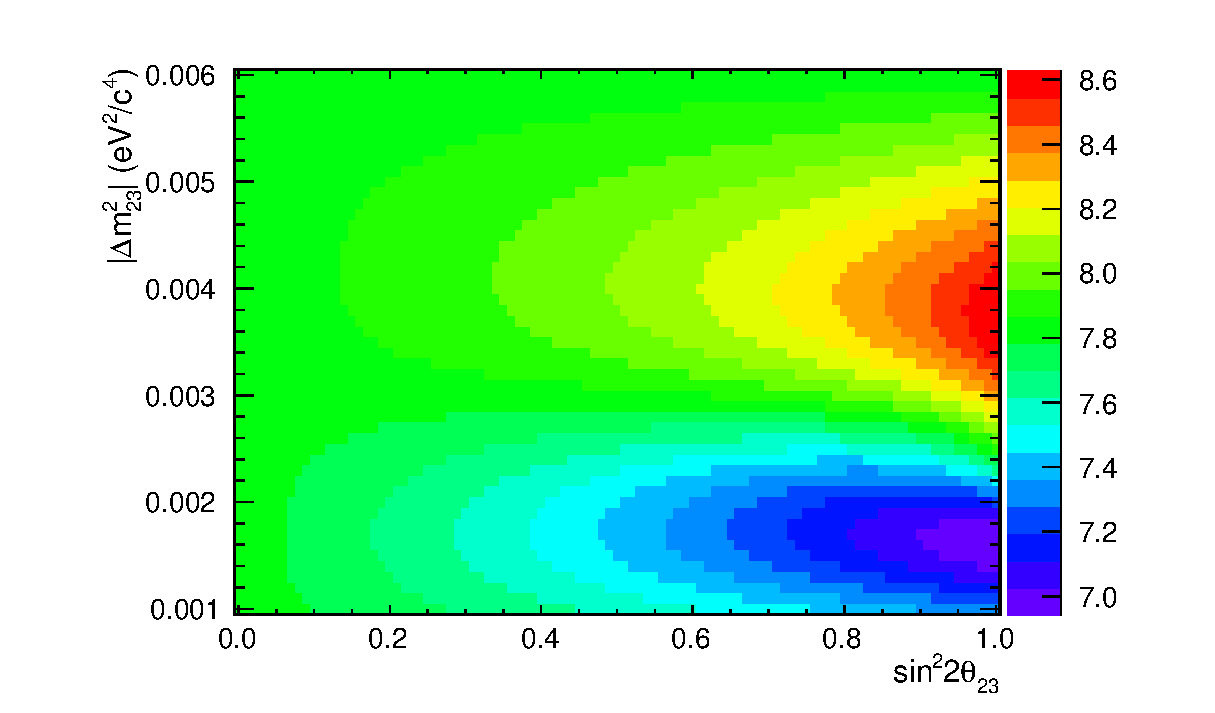
\includegraphics[width=38pc]{./images/predicted_spectrum/systematic_variations/frac_nsk_err_twk_xsec.eps}
\caption{
  Percentage uncertainty
  on expected numbers of 1-ring $\mu$-like events (after extrapolation)
  in the 0-10 GeV reconstructed energy range
  due to quoted cross uncertainties only.
  Over the oscillation parameter space considered by this analysis, 
  the uncertainty in the 7\% to 8.6\% range.
  This plot can be directtly compared 
  with the GENIE-NEUT difference shown in Fig. \ref{fig:genie_neut_nsk_difference_osc_param_grid}.
}
\label{fig:nsk_uncertainty_osc_param_grid_xsec_err_only}
\end{figure*}
  

\subsection {Evaluating systematics at oscillation best-fit point}
\label{sec:systematics_at_osc_bestfit}

Systematics, at a given point of the oscillation parameter space, are calculated by 
fitting a large number (typically 10,000) of toy experiments, generated with the 
given oscillation parameters and with randomly varied systematic parameters.
The systematic error on $sin^{2}2\theta_{23}$ and $\Delta m^{2}_{23}$ 
are taken to be the one standard deviation of the corresponding best-fit parameter distribution.
In order to decouple statistical and systematic effects, 
no statistical fluctuations are included in the toy experiments.
The effect of each systematic parameter is calculated separately
and then they are combined by adding them in quadratures.
An evaluation of the 3.23$\times 10^{19}$-POT T2K disapearance analysis systematics for 
oscillation parameters near the MINOS best fit point 
($sin^{2}2\theta_{23}$ = 0.9 and $\Delta m^{2}_{23}$ = 2.4$\times10^{-3}$ $eV^{2}/c^{4}$)
is shown in Tab. \ref{table:systamatics_at_2p4Em3_0p9}.

\begin{table*}[htb]
\center
\renewcommand{\arraystretch}{1.75} % enlarge line spacing
\begin{tabular}{|c|cc|cc|}
\hline
              &
  \multicolumn{2}{c|} { GENIE } &
  \multicolumn{2}{c|} { NEUT  } \\
Error source  &
  $\Big(\frac{\delta{\Delta m^{2}_{23}}}{\Delta m^{2}_{23}}\Big)$  & $\Big(\frac{\delta{\sin^{2}2\theta_{23}}}{sin^{2}2\theta_{23}}\Big)$  &
  $\Big(\frac{\delta{\Delta m^{2}_{23}}}{\Delta m^{2}_{23}}\Big)$  & $\Big(\frac{\delta{\sin^{2}2\theta_{23}}}{sin^{2}2\theta_{23}}\Big)$  \\
\hline
SuperK CCQE efficiency            &   0.3\%   &   1.7\%      &   0.5\%   &   1.6\%  \\
SuperK CCnonQE efficiency         &   0.5\%   &   1.1\%      &   0.5\%   &   1.3\%  \\
SuperK NC efficiency              &   3.9\%   &   3.1\%      &   3.5\%   &   3.0\%  \\
SuperK $\nu_{e}$ CC efficiency    &   0.0\%   &   0.0\%      &   0.0\%   &   0.0\%  \\
SuperK energy scale               &   0.3\%   &   0.2\%      &   0.5\%   &   0.2\%  \\
ND280 efficiency                  &   0.1\%   &   1.5\%      &   0.3\%   &   1.4\%  \\
Flux normalization                &   0.1\%   &   1.6\%      &   0.3\%   &   1.5\%  \\
Flux shape                        &   2.3\%   &   0.5\%      &   2.2\%   &   0.6\%  \\
CCQE cross section                &   1.2\%   &   1.5\%      &   1.0\%   &   1.5\%  \\
CC1pi/CCQE cross section ratio    &   0.2\%   &   0.6\%      &   0.1\%   &   0.3\%  \\
CCother/CCQE cross section ratio  &   0.1\%   &   1.7\%      &   0.1\%   &   1.5\%  \\
NC/CCQE cross section ratio       &   1.2\%   &   0.5\%      &   1.2\%   &   0.5\%  \\
FSI                               &   0.1\%   &   0.7\%      &   0.3\%   &   0.6\%  \\
\hline
Total                             &   5.1\%   &   5.3\%      &   4.7\%   &   5.0\%  \\
\hline
\end{tabular}\\[2pt]
\caption{
  Oscillation systematics evaluated at
  $sin^{2}2\theta_{23}$ = 0.9 and $\Delta m^{2}_{23}$ = 2.4$\times10^{-3}$ $eV^{2}/c^{4}$.
}
\label{table:systamatics_at_2p4Em3_0p9}
\end{table*}


\subsection {Including systematics in calculation of confidence regions}

In the context of the Feldman-Cousins analysis, systematic errors are naturally included in
the confidence regions by including systematic variations in the toy experiments used for
calculating the $\Delta\chi^{2}_{a}$ surfaces (where $a$ denotes the specified confidence level)
as a function of $sin^{2}2\theta_{23}$ and $\Delta m^{2}_{23}$. 
The procedure was outlined in Sec. \ref{sec:contour_fc}.

\subsection {Handling correlated systematics: Cholesky decomposition method}
\label{sec:cholesky}

The LU decomposition is a well-known factorization of a matrix ${\bf C}$
as a product of a lower triangular matrix ${\bf L}$ and an upper triangular matrix ${\bf U}$.
The LU decomposition has several applications in scientific computing \cite{NumRecipCholesky}.
Let ${\bf C}$ be a square, symmetric, positive-definite\footnote{
  ${\bf v} \cdot {\bf C} \cdot {\bf v} > 0$ for every vector ${\bf v}$.} matrix.
Under the stated conditions, there exists a special factorization of ${\bf C}$, the Cholesky decomposition,
which is significantly {\em more efficient} than the generic LU decomposition.
Rather than factorizing ${\bf C}$ as the product of two independent matrices ${\bf L}$ and ${\bf U}$,
the Cholesky method factorizes ${\bf C}$ as the product 
of a lower triangular matrix ${\bf L}$ and its transpose matrix:
\begin{equation}
\displaystyle 
  {\bf C} = {\bf L} \cdot {\bf L}^{T} 
\end{equation}
The Cholesky decomposition algorithm can be found in \cite{NumRecipCholesky}.

The Cholesky decomposition is commonly used for Monte Carlo simulation of systems with correlated variables.
Let $S_{N}$ be such a system whose dimensionality is $N$
and let ${\bf C}$ be the $N \times N$ matrix which describes the covariance of the 
$N$ simulated variables.
The covariance matrix ${\bf C}$ is decomposed to obtain the lower triangular matrix ${\bf L}$.
Let ${\bf u}$ be a $N$-dimensional vector of uncorrelated variables;
each vector element $u_{i}$ can be randomly generated from a gaussian
distribution with a mean of 0 and a standard deviation of 1.
The vector
\begin{equation}
\displaystyle 
  {\bf x} = {\bf L} \cdot {\bf u}
\end{equation}
has the covariance properties of $S_{N}$.



\section {Oscillation fit to the $3.23\times10^{19}$ POT dataset}
\label{sec:oscfit_runI}

Using the method outlined in the previous sections,
an oscillation fit was performed to the 2010a $3.23\times10^{19}$ POT dataset.
For GENIE, this analysis finds
$|\Delta m^{2}_{23}|$ = 2.8$\times$10$^{-3}$ $eV^{2}/c^{4}$ and
$sin^{2}2\theta_{23}$ = 0.81
as the best-fit values.
For NEUT, the corresponding values are
$|\Delta m^{2}_{23}|$ = 2.9$\times$10$^{-3}$ $eV^{2}/c^{4}$ and
$sin^{2}2\theta_{23}$ = 0.83.
The reconstructed neutrino energy distribution for the 8 1-ring $\mu$-like events of the 
2010a dataset, along with the best-fit predictions from GENIE and NEUT are shown in  
Figs. \ref{fig:fit2010a_spectrum_and_data_genie} and \ref{fig:fit2010a_spectrum_and_data_neut}.

The systematic errors at the best-fit point were evaluated as described in 
Sec. \ref{sec:systematics_at_osc_bestfit}.
The systematic errors at the GENIE best-fit point are given, 
in Tab. \ref{table:oscsyst_at_genie_bestfit_point}. 
For NEUT, the systematic errors at the best-fit point
are given in Tab. \ref{table:oscsyst_at_neut_bestfit_point}.
We list the effect on $|\Delta m^{2}_{23}|$ and $sin^{2}2\theta_{23}$ of
all systematic uncertainties considered in this analysis.
The total systematic error is computed by adding 
in quadrature
the errors due to individual systematic uncertainties.
This analysis finds that the combined systematic uncertainty at the GENIE (NEUT) best-fit point 
is 4.3\% (3.9\%) for $|\Delta m^{2}_{23}|$ and 6.7\% (6.0\%) for $sin^{2}2\theta_{23}$.
The SuperK NC efficiency, the CCQE cross section and the flux shape uncertainties 
are the ones with the largest impact on $|\Delta m^{2}_{23}|$.
The dominant systematics on $sin^{2}2\theta_{23}$ are the SuperK CCQE efficiency,
the flux normalization, the ND280 efficiency and the CCother/CCQE cross section ratio.

Confidence regions were calculated using both methods described in Sec. \ref{sec:contours}.
A comparison of the Feldman-Cousins and plain confidence regions (including statistical errors only) 
for the 2010a dataset is shown in Fig. \ref{fig:fit2010a_compare_fc_nonfc_statonly}.
As discussed in Sec. \ref{sec:contours} the Feldman-Cousins confidence regions have correct coverage 
by construction. 
As it can be seen in Fig. \ref{fig:fit2010a_compare_fc_nonfc_statonly},
the Feldman-Cousins and plain confidence regions differ significantly
and, therefore, the coverage of the latter is spurious.
The plain confidence regions tend to overcover near a physical boundary, and either
undercover or overcover away from that boundary. 
Consequently, this analysis considers only the Feldman-Cousins method for quoting
the final results.
The 68\%, 90\% and 95\% Feldman-Cousins confidence regions, with and without systematics, for the 2010a
$\nu_{\mu}$ disappearance analysis are shown in
Fig. \ref{fig:fit2010a_confregion_genie} for GENIE and in
Fig. \ref{fig:fit2010a_confregion_neut} for NEUT.
The estimated systematic error at the best-fit point 
(listed in Tabs. \ref{table:oscsyst_at_genie_bestfit_point} and \ref{table:oscsyst_at_neut_bestfit_point})
is also shown.

Upon seeing the reconstructed energy distribution of the 2010a dataset, it was clear to the authors
of this note that large values of $|\Delta m^{2}_{23}|$, in the wrong trough of the oscillation survival
probability function, may provide a better fit to the data.
The oscillation parameter limits (discussed in Sec. \ref{sec:osc_par_limits}) were relaxed and a new fit
was performed. The result is shown in Fig. \ref{fig:fit2010a_wide_dmsq_genie}.
Indeed, a better fit to the data exists at maximal mixing angle and
large $|\Delta m^{2}_{23}|$ (of the order of 10$^{-2}$ eV$^{2}$/c$^{4}$,
some $\sim$ 20$\sigma$ away from the MINOS best-fit value).
As it can be seen in Fig. \ref{fig:fit2010a_wide_dmsq_genie},
much of the $\chi^{2}$ valley at large $|\Delta m^{2}_{23}|$, is lower than the
best-fit point in the 
$|\Delta m^{2}_{23}|$ window
from 10$^{-3}$ eV$^{2}$/c$^{4}$ to 6$\times$10$^{-3}$ eV$^{2}$/c$^{4}$.
Fig. \ref{fig:fit2010a_wide_dmsq_marginalised_genie} shows 
the marginalised $\chi^{2}$ distributions from the fit shown in Fig. \ref{fig:fit2010a_wide_dmsq_genie}.

Although the high $|\Delta m^{2}_{23}|$ solution was pointed-out by the authors of this analysis,
the majority of the authors feel uneasy modifying the pre-defined analysis procedure 
after seeing the actual data (in response to a statistical fluctuation in the observed dataset).
The pre-defined $|\Delta m^{2}_{23}|$ limits of 1$\times$10$^{-3}$ eV$^{2}$/c$^{4}$ and 6$\times$10$^{-3}$ eV$^{2}$/c$^{4}$
correspond to the T2K sensitivity window, as it can be seen clearly in Fig. \ref{fig:sk_spectrum_sensitivity_limits_and_highDm2}.
The limits were set (before looking at the data) exactly so as to avoid fluctuations such as the one observed in the data.
This entire experiment (and analysis) was built on the premise that the first oscillation minimum is around the T2K peak energy,
as was determined by MINOS and K2K. 
In addition, including this prior knowledge (Bayesian prior) into the oscillation result does
not invalidate the frequentist interpretation of the confidence regions as it has been incorrectly indicated \cite{Mauro}.
The SuperK expectation already employs a host of other Bayesian priors;
they are physics parameters, such as the quasi-elastic axial mass, which are selected based on belief from
(sometimes) conflicting experimental results.
Still, one can certainly assert that the 68\% confidence regions shown in this analysis is the region where 68\% of the 
measurements would fall if the same measurement could be repeated N times. 
The statement implies analysing N independent 3.23E+19 POT datasets using the exact same input assumptions (Bayesian priors).
The confidence regions shown here have correct coverage and proper frequestist interpretation 
in the $|\Delta m^{2}_{23}|$ window
from 10$^{-3}$ eV$^{2}$/c$^{4}$ to 6$\times$10$^{-3}$ eV$^{2}$/c$^{4}$.
The arguments against showing confidence regions from a fit to an enlarged $|\Delta m^{2}_{23}|$ range were made 
convincingly in \cite{DeanAndNick} and will not be repeated here. 
For the actual publication it is proposed that 
a) we show the best-fit value and confidence regions in the restricted $|\Delta m^{2}_{23}|$ range, and 
b) we indicate the existence of a global minimum outside the restricted $|\Delta m^{2}_{23}|$ range
   and we quote the probability for such a fluctuation.
The probability for such a $|\Delta m^{2}_{23}|$ fluctuation with a $3.23\times10^{19}$ POT exposure is
about 5.6\% (see Fig. \ref{fig:dmsq-distribution-2p35Em3-1p0-1x}). With $1\times10^{20}$ POT (dataset already accumulated at the time of revisiting
this note) the probability for such a fluctuation has already fallen to about 0.2\% (see Fig. \ref{fig:dmsq-distribution-2p35Em3-1p0-3x}).

\begin{table*}[htb]
\center
\renewcommand{\arraystretch}{1.75} % enlarge line spacing
\begin{tabular}{|c|cc|}
\hline
Error source  &
  $\Big(\frac{\delta{\Delta m^{2}_{23}}}{\Delta m^{2}_{23}}\Big)$  & $\Big(\frac{\delta{\sin^{2}2\theta_{23}}}{sin^{2}2\theta_{23}}\Big)$  \\
\hline
SuperK CCQE efficiency            &   0.5\%   &   2.9\%      \\
SuperK CCnonQE efficiency         &   1.0\%   &   1.6\%      \\
SuperK NC efficiency              &   2.0\%   &   1.8\%      \\
SuperK $\nu_{e}$ CC efficiency    &   0.0\%   &   0.0\%      \\
SuperK energy scale               &   0.5\%   &   0.3\%      \\
ND280 efficiency                  &   0.2\%   &   2.2\%      \\
Flux normalization                &   0.3\%   &   2.8\%      \\
Flux shape                        &   2.6\%   &   1.0\%      \\
CCQE cross section                &   1.8\%   &   1.8\%      \\
CC1pi/CCQE cross section ratio    &   1.1\%   &   1.1\%      \\
CCother/CCQE cross section ratio  &   0.4\%   &   2.6\%      \\
NC/CCQE cross section ratio       &   0.5\%   &   0.1\%      \\
FSI                               &   0.2\%   &   1.1\%      \\
\hline
Total                             &   4.3\%   &   6.7\%      \\
\hline
\end{tabular}\\[2pt]
\caption{
  Oscillation systematics computed using GENIE, at the GENIE best-fit point
  ($sin^{2}2\theta_{23}$ = 0.81 and $\Delta m^{2}_{23}$ = 2.8$\times10^{-3}$ $eV^{2}/c^{4}$).
}
\label{table:oscsyst_at_genie_bestfit_point}
\end{table*}


\begin{table*}[htb]
\center
\renewcommand{\arraystretch}{1.75} % enlarge line spacing
\begin{tabular}{|c|cc|}
\hline
Error source  &
  $\Big(\frac{\delta{\Delta m^{2}_{23}}}{\Delta m^{2}_{23}}\Big)$  & $\Big(\frac{\delta{\sin^{2}2\theta_{23}}}{sin^{2}2\theta_{23}}\Big)$  \\
\hline
SuperK CCQE efficiency            &   0.6\%   &   2.6\%      \\
SuperK CCnonQE efficiency         &   1.0\%   &   1.7\%      \\
SuperK NC efficiency              &   1.6\%   &   1.5\%      \\
SuperK $\nu_{e}$ CC efficiency    &   0.0\%   &   0.0\%      \\
SuperK energy scale               &   0.5\%   &   0.4\%      \\
ND280 efficiency                  &   0.2\%   &   2.1\%      \\
Flux normalization                &   0.3\%   &   2.6\%      \\
Flux shape                        &   2.3\%   &   1.1\%      \\
CCQE cross section                &   1.7\%   &   1.4\%      \\
CC1pi/CCQE cross section ratio    &   1.0\%   &   0.8\%      \\
CCother/CCQE cross section ratio  &   0.5\%   &   2.1\%      \\
NC/CCQE cross section ratio       &   0.4\%   &   0.1\%      \\
FSI                               &   0.4\%   &   1.1\%      \\
\hline
Total                             &   3.9\%   &   6.0\%      \\
\hline
\end{tabular}\\[2pt]
\caption{
  Oscillation systematics computed using NEUT, at the NEUT best-fit point
  ($sin^{2}2\theta_{23}$ = 0.83 and $\Delta m^{2}_{23}$ = 2.9$\times10^{-3}$ $eV^{2}/c^{4}$).
}
\label{table:oscsyst_at_neut_bestfit_point}
\end{table*}



\begin{figure*}[htb]
\center
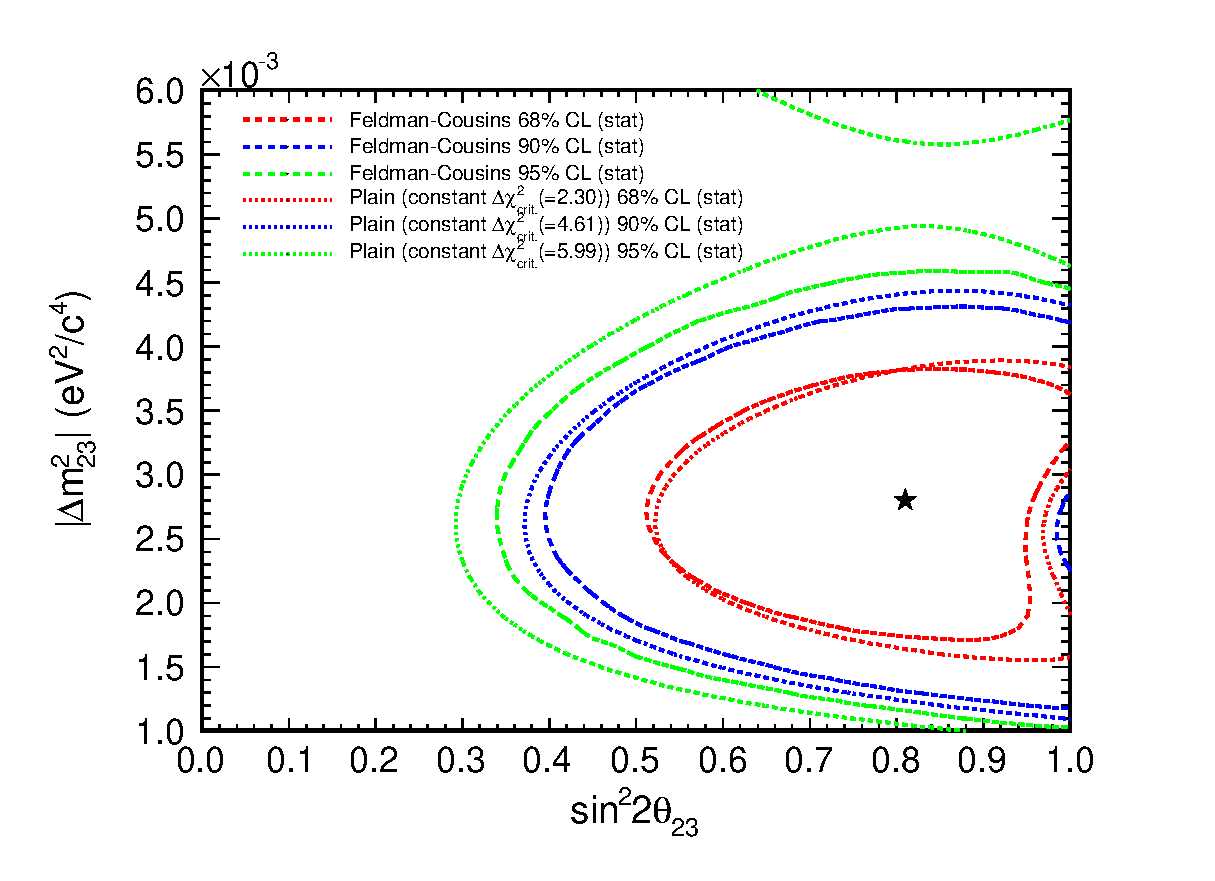
\includegraphics[width=42pc]{./images/fits/2010a/contour_stat_genie_compare_fc_nonfc.eps}
\caption{
 Comparison of the Feldman-Cousins and plain confidence regions (including statistical errors only)
 for the 2010a dataset. As discussed in Sec. \ref{sec:contours} the Feldman-Cousins confidence regions 
 have correct coverage by construction. 
 The Feldman-Cousins and plain confidence regions differ significantly and, therefore,
 coverage of the plain contours is spurious. The latter seem to overcover significantly
 near the physical boundary and undercover away from it.
 In addition, the non plain contour appears to ignore the existence of $\Delta m^{2}_{23}$ boundaries
 (fitter limits). 
 The contours are shown for GENIE.
 Identical conclusions are drawn by the comparison of the Feldman-Cousins and plain confidence regions 
 generated by NEUT.
}
\label{fig:fit2010a_compare_fc_nonfc_statonly}
\end{figure*}

\begin{figure*}[htb]
\center
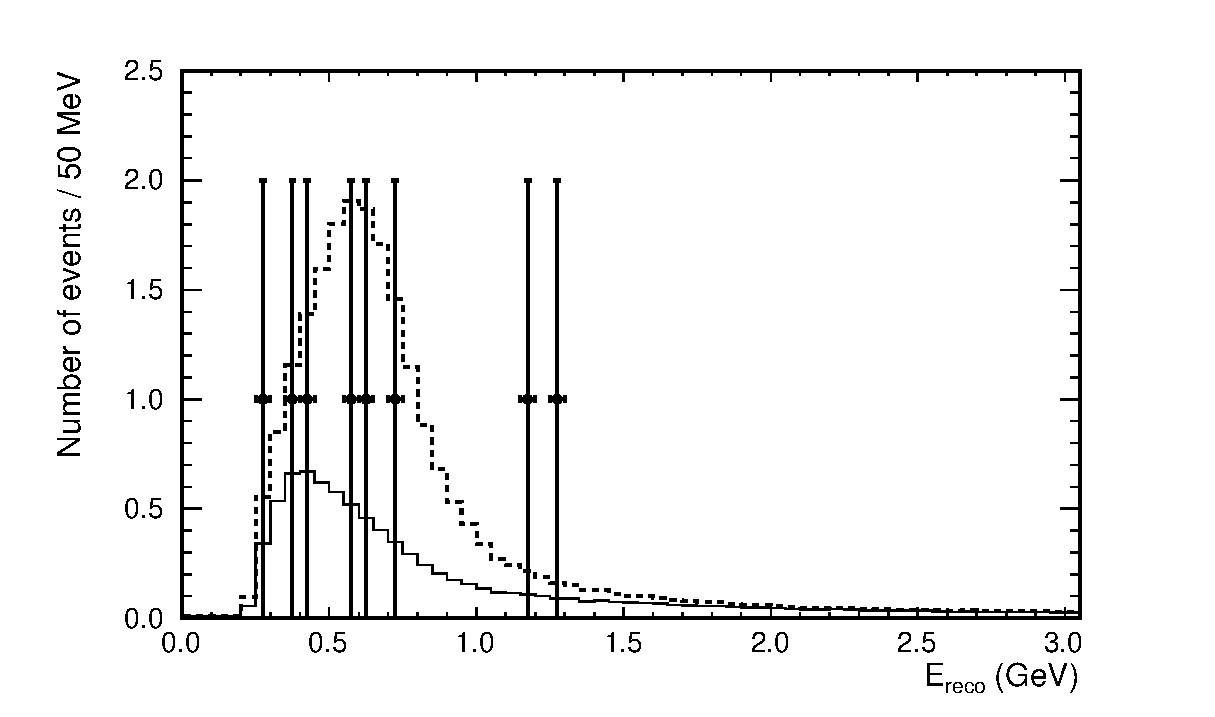
\includegraphics[width=28pc]{./images/fits/2010a/genie_bestfit_spectrum.eps}
\caption{
  Reconstructed neutrino energy distribution for the 8 1-ring $\mu$-like events of the 
  2010a 3.23$\times$10$^{19}$ POT dataset (points) and GENIE best-fit SuperK prediction (solid line).
  The best-fit oscillation parameters (in the search window defined in Sec. \ref{sec:osc_par_limits}) are 
  $|\Delta m^{2}_{23}|$ = 2.8$\times$10$^{-3}$ $eV^{2}/c^{4}$ and $sin^{2}2\theta_{23}$ = 0.81.
  The dotted line shows the GENIE prediction without oscillations.
}
\label{fig:fit2010a_spectrum_and_data_genie}
\end{figure*}

\begin{figure*}[htb]
\center
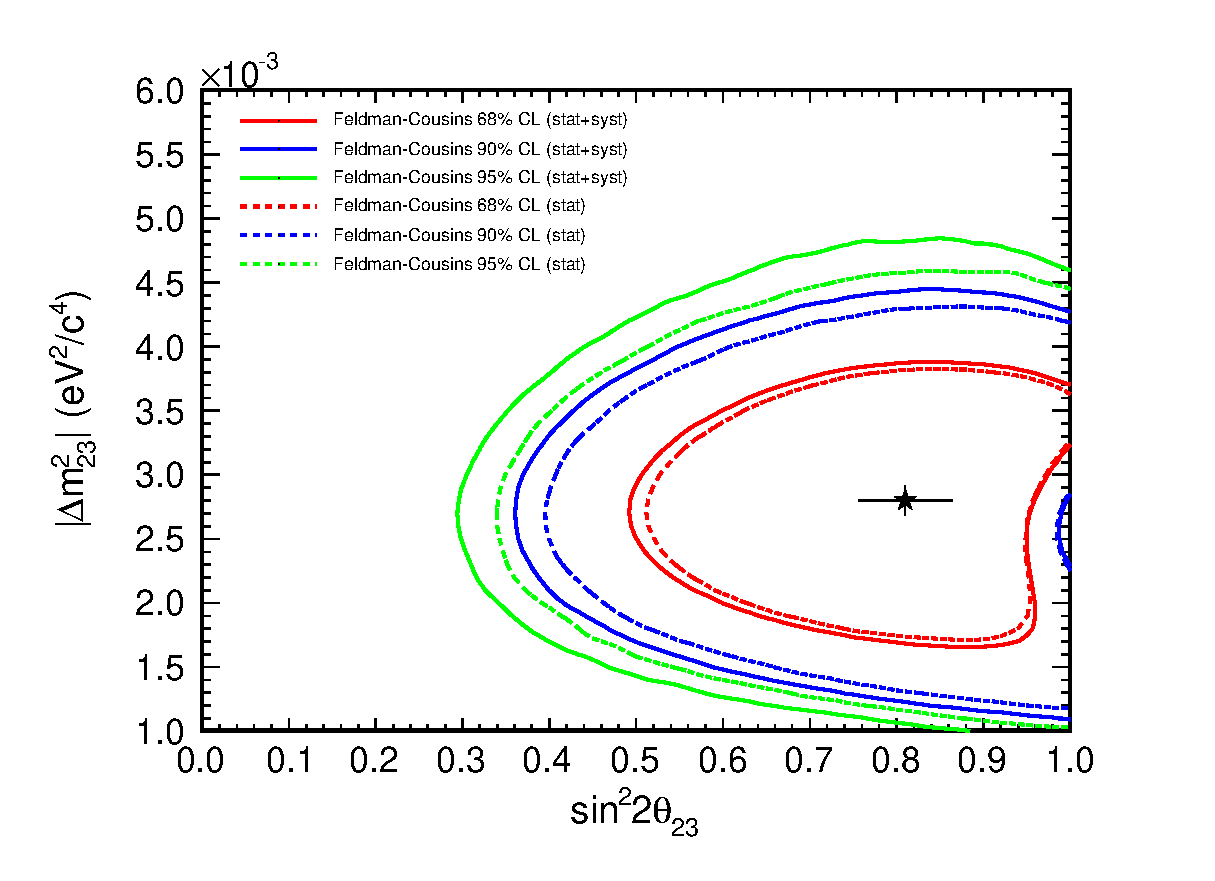
\includegraphics[width=36pc]{./images/fits/2010a/contour_statsyst_andbestfitsyst_genie.eps}
\caption{
  68\%, 90\% and 95\% Feldman-Cousins confidence regions, with and without systematics,
  for the GENIE disappearance fit to the 2010a dataset.
  The estimated systematic error at the best-fit point is also shown with a cross.
}
\label{fig:fit2010a_confregion_genie}
\end{figure*}

\begin{figure*}[htb]
\center
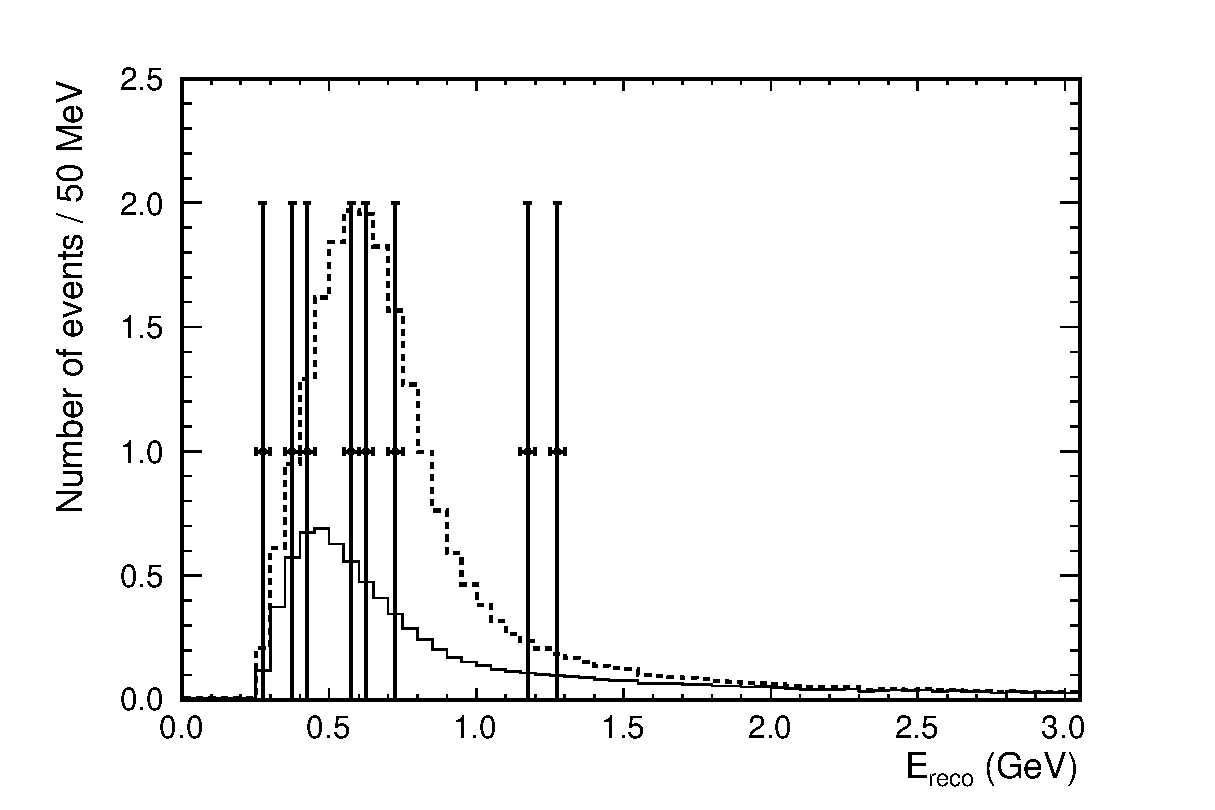
\includegraphics[width=28pc]{./images/fits/2010a/neut_bestfit_spectrum.eps}
\caption{
  Reconstructed neutrino energy distribution for the 8 1-ring $\mu$-like events of the 
  2010a 3.23$\times$10$^{19}$ POT dataset (points) and NEUT best-fit SuperK prediction (solid line).
  The best-fit oscillation parameters (in the search window defined in Sec. \ref{sec:osc_par_limits}) are 
  $|\Delta m^{2}_{23}|$ = 2.9$\times$10$^{-3}$ $eV^{2}/c^{4}$ and $sin^{2}2\theta_{23}$ = 0.83.
  The dotted line shows the NEUT prediction without oscillations.
}
\label{fig:fit2010a_spectrum_and_data_neut}
\end{figure*}

\begin{figure*}[htb]
\center
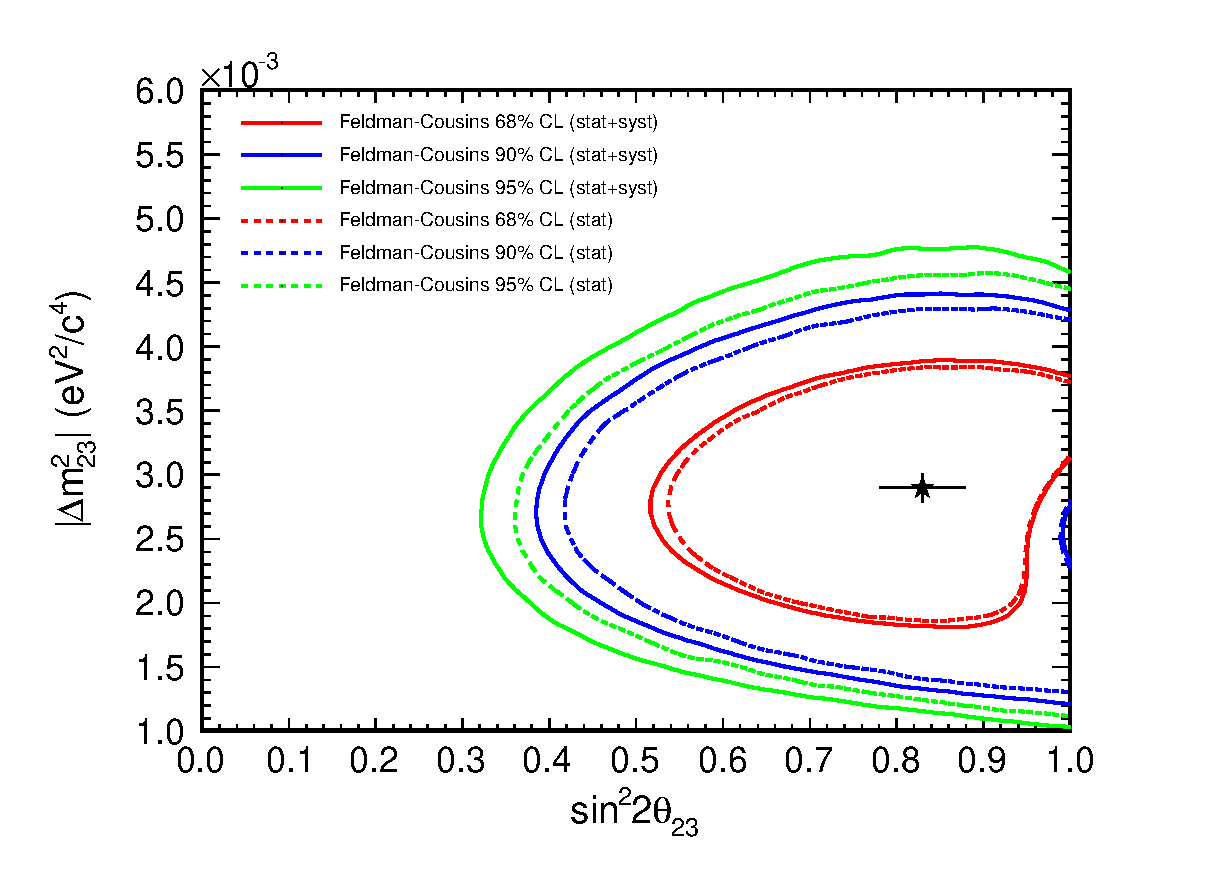
\includegraphics[width=36pc]{./images/fits/2010a/contour_statsyst_andbestfitsyst_neut.eps}
\caption{
  68\%, 90\% and 95\% Feldman-Cousins confidence regions, with and without systematics,
  for the NEUT disappearance fit to the 2010a dataset.
  The estimated systematic error at the best-fit point is also shown with a cross.
}
\label{fig:fit2010a_confregion_neut}
\end{figure*}


\begin{figure*}[htb]
\center
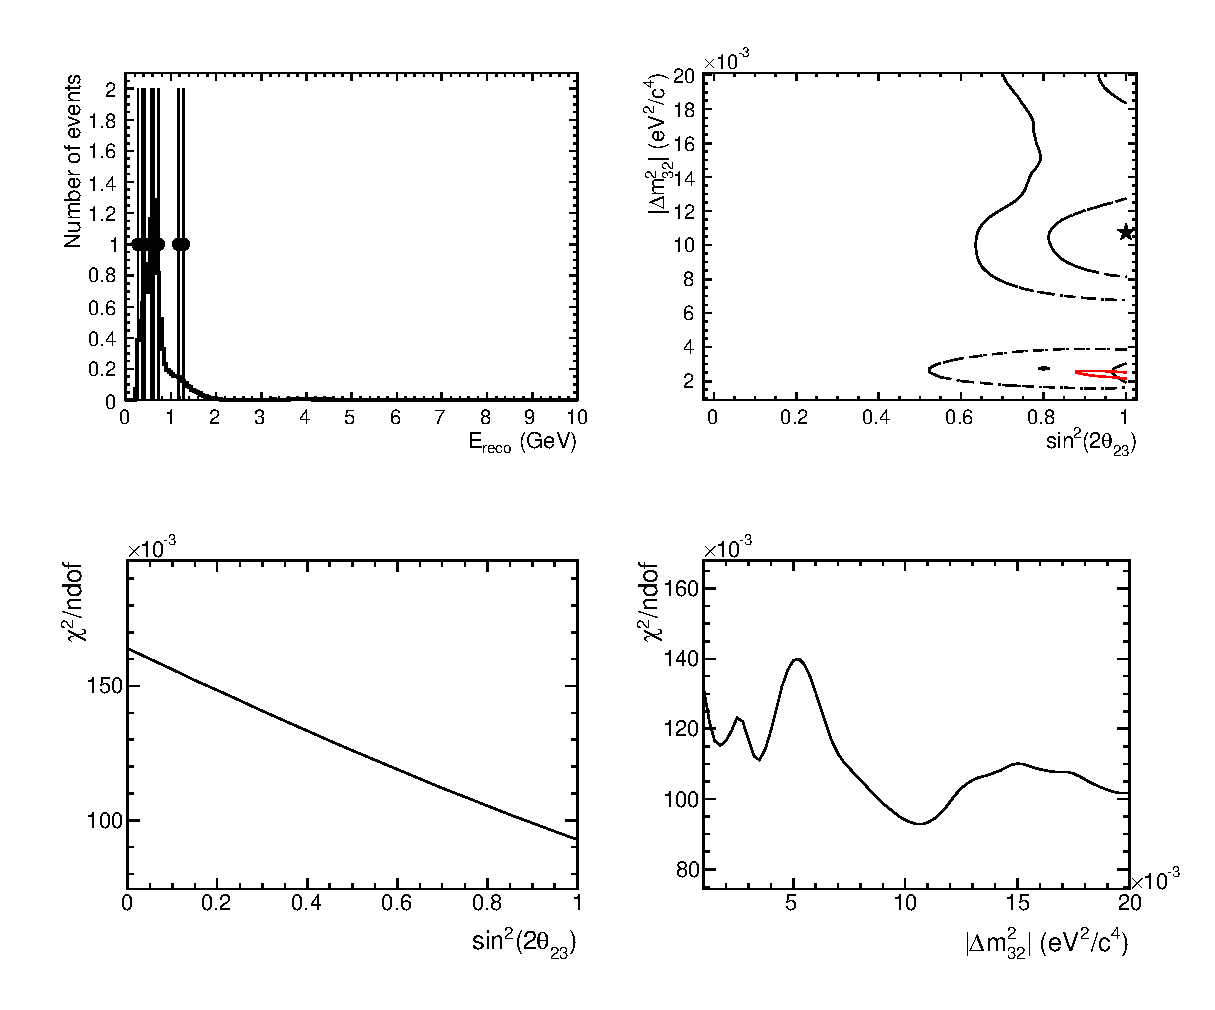
\includegraphics[width=28pc]{./images/fits/2010a/fit_2010a_genie_wide.eps}
\caption{
  Fit to the 2010a set with relaxed upper limit of $|\Delta m^{2}_{23}|$.
  The top-left plot shows the reconstructed energies of the 2010a dataset and the best-fit prediction.
  The confidence regions shown on the top-right are the 68\% and 90\% CL regions (statistical errors only) 
  calculated, for simplicity, using the PDG method.
  For reference, the MINOS 90\% CL region is also shown (red line).
  The best-fit point is shown with a black-star.
  The bottom-left and bottom-right plots show the $\chi^{2}$/ndof along the $sin^{2}2\theta_{23}$ and $|\Delta m^{2}_{23}|$
  lines that pass through the best-fit point.
}.
\label{fig:fit2010a_wide_dmsq_genie}
\end{figure*}

\begin{figure*}[htb]
\center
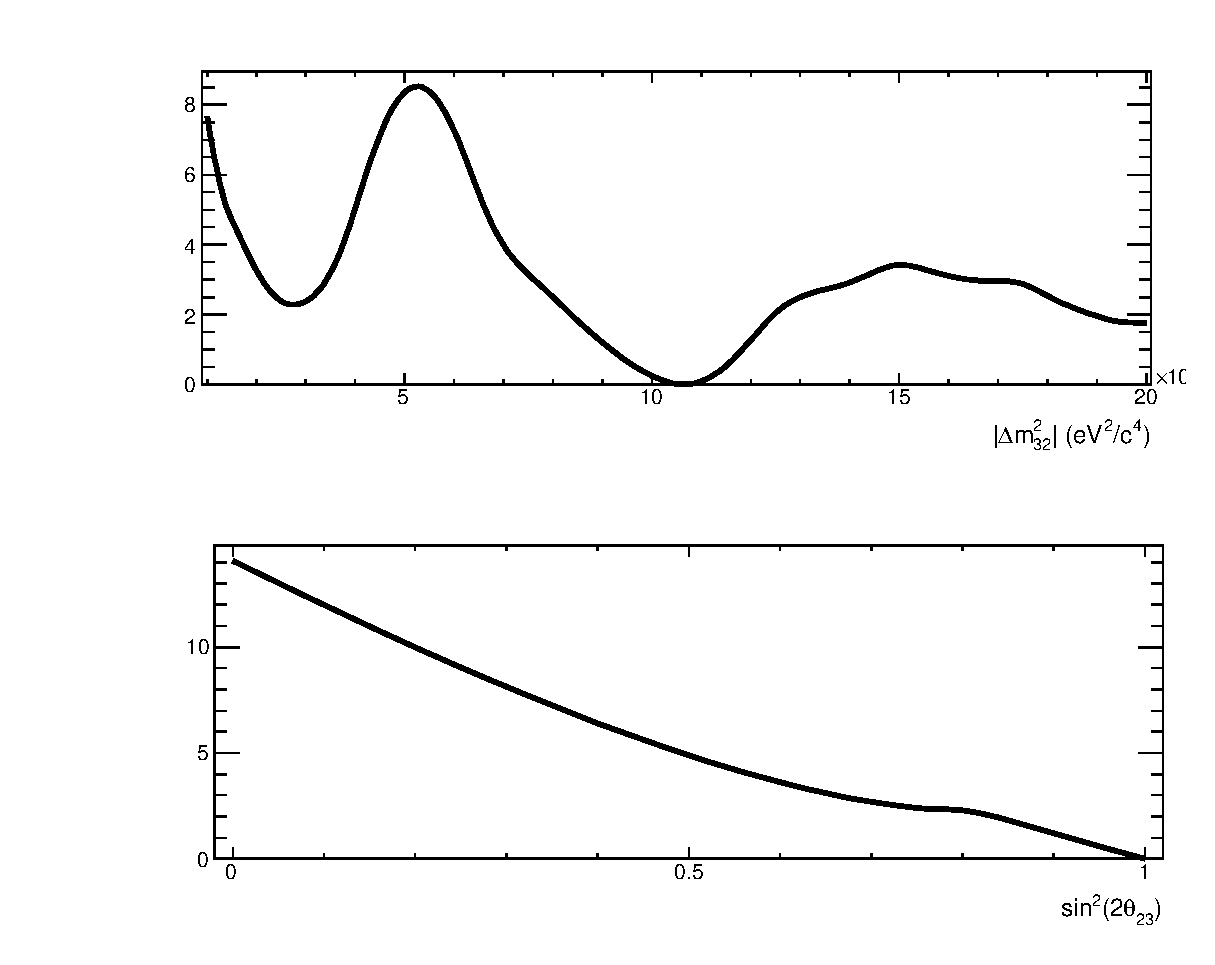
\includegraphics[width=24pc]{./images/fits/2010a/fit_2010a_genie_wide_marginalised_chisq.eps}
\caption{
  Marginalised $\chi^{2}$ distributions for the fit shown in Fig. \ref{fig:fit2010a_wide_dmsq_genie}.
}
\label{fig:fit2010a_wide_dmsq_marginalised_genie}
\end{figure*}


\begin{figure*}[htb]
\center
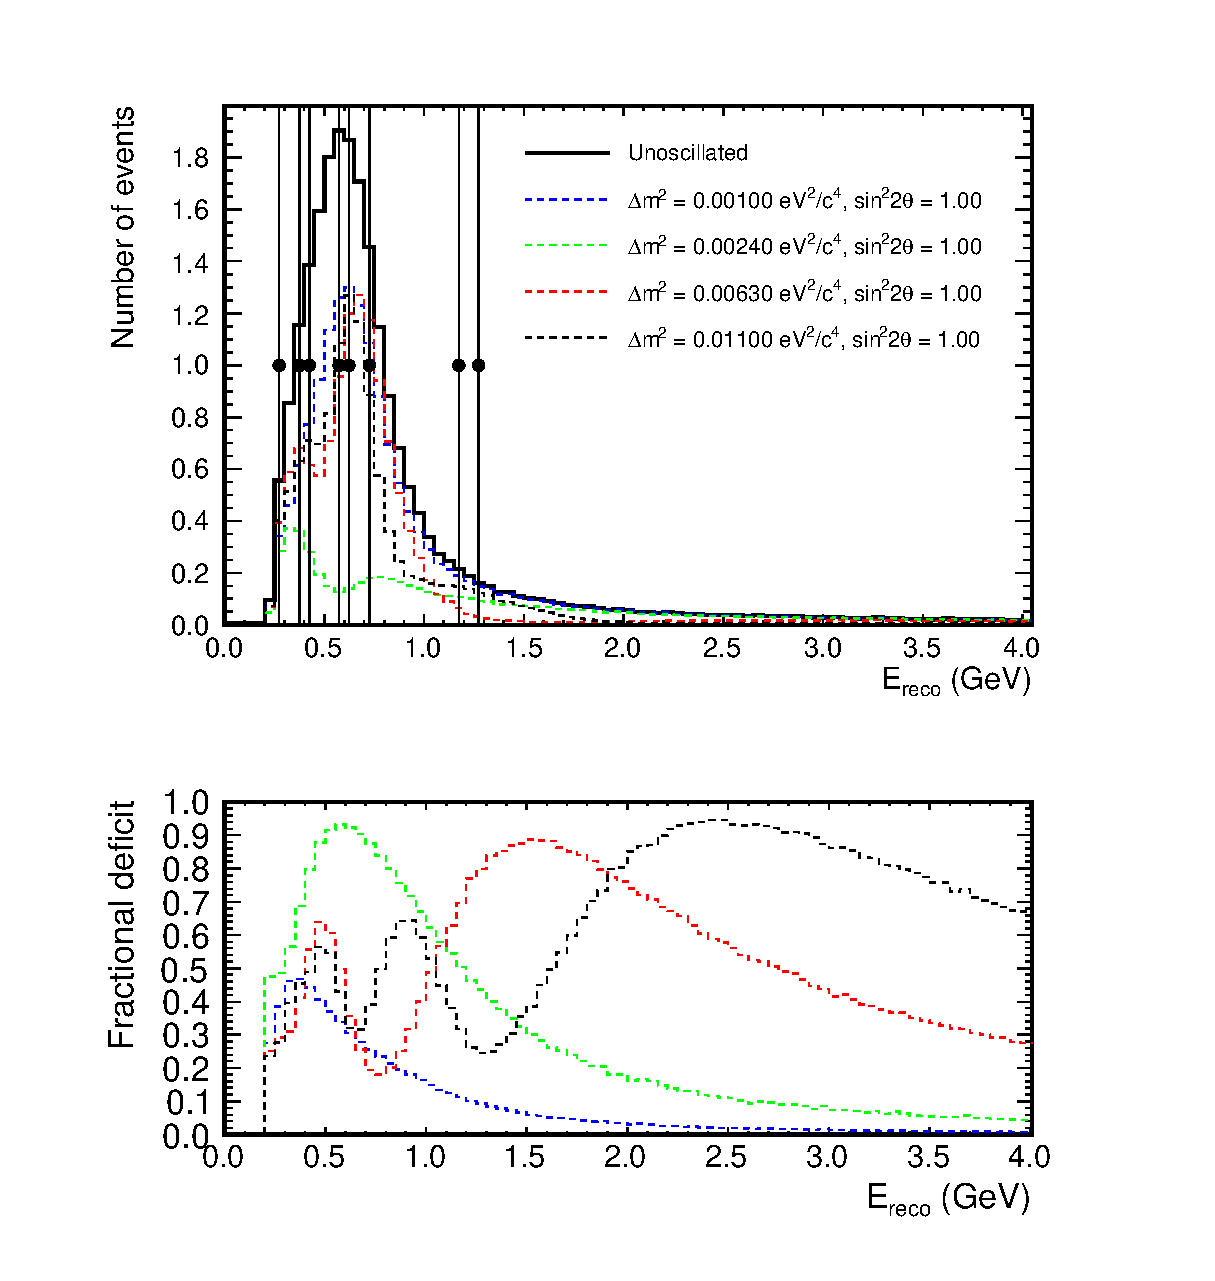
\includegraphics[width=38pc]{./images/etc/sk_spectrum_sensitivity_limits_and_highDm2_data.eps}
\caption{
  Predicted reconstructed-energy spectrum of 1-ring $\mu$-like events (after extrapolation)
  for $sin^{2}2\theta_{23}$ = 1.0 and
  $\Delta m^{2}_{23}$ =
    1.0$\times10^{-3}$ $eV^{2}/c^{4}$,
    2.4$\times10^{-3}$ $eV^{2}/c^{4}$,
    6.0$\times10^{-3}$ $eV^{2}/c^{4}$ and
    1.1$\times10^{-2}$ $eV^{2}/c^{4}$.
  The non-oscillated spectrum (GENIE) and the 2010a dataset are also shown.
  With $|\Delta m^{2}_{23}|$ = 1$\times$10$^{-3}$ eV$^{2}$/c$^{4}$ the first oscillation minimum is in the region dominated by
  NC and non-CCQE interactions. On the other hand, with $|\Delta m^{2}_{23}|$ = 6$\times$10$^{-3}$ eV$^{2}$/c$^{4}$ the (first) 
  oscillation minimum is already well above the T2K peak energy. In both of these cases, our $|\Delta m^{2}_{23}|$ messurement 
  capabilities are much deteriorated. With $\Delta m^{2}_{23}$=1.1$\times10^{-2}$ $eV^{2}/c^{4}$, the first oscillation minimum 
  appears at 2.5 GeV! The high-$\Delta m^{2}_{23}$ solution provides a better fit to the small 2010a dataset only because the 
  second and third oscillation minina happen to be accomodated between gaps (pseudo-dips) left by the 8 observed events at
  around 0.5 GeV and 1 GeV. The probability for such a $\Delta m^{2}_{23}$ fluctuation is given in the text.
}
\label{fig:sk_spectrum_sensitivity_limits_and_highDm2}
\end{figure*}

\begin{figure*}[htb]
\center
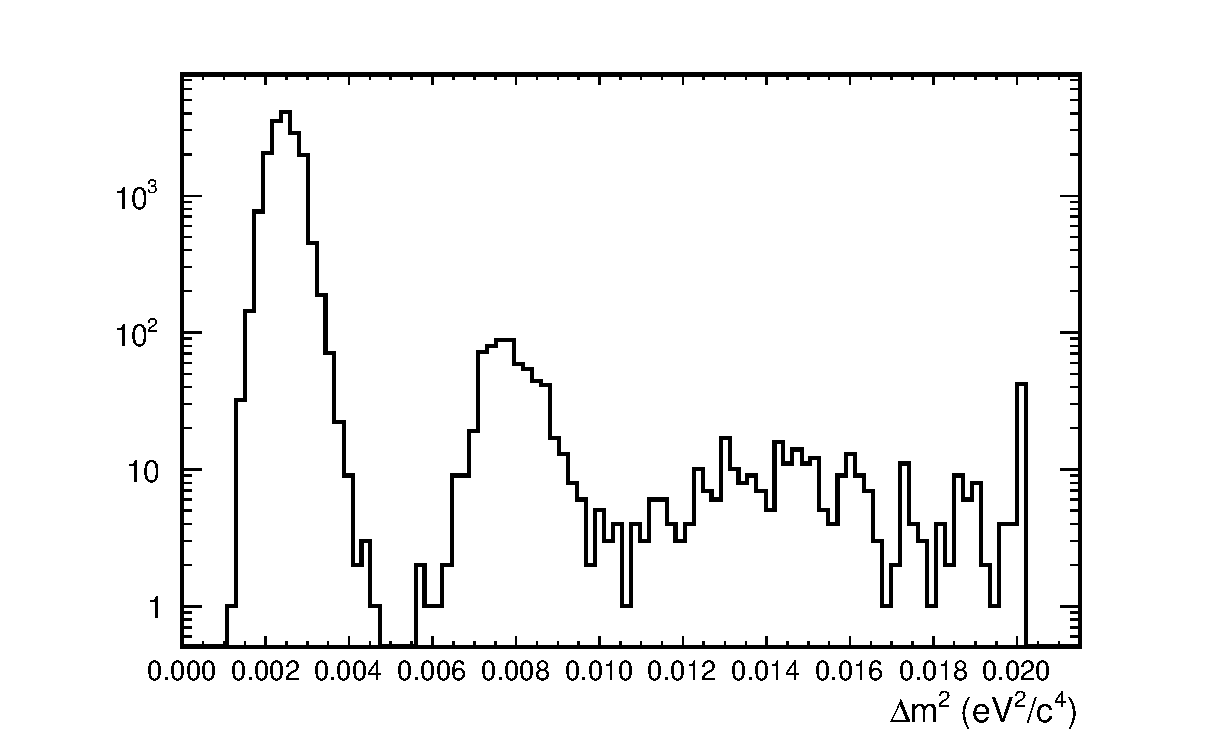
\includegraphics[width=27pc]{./images/etc/dmsq-distribution-2p35Em3-1p0-1x.eps}
\caption{
  Distribution of best-fit $\Delta m^{2}_{23}$ values for a set of toy MC experiments
  generated with the MINOS best-fit values ($\Delta m^{2}_{23}$ = 2.35$\times10^{-3}$ $eV^{2}/c^{4}$
  and maximal mixing). The toy MC experiments were generated for an 
  integrated neutrino beam exposure of $3.23\times10^{19}$ POT and systematic variations were included.
  5.6\% of fits gave a $\Delta m^{2}_{23}$ value above 6$\times10^{-3}$ $eV^{2}/c^{4}$.
}
\label{fig:dmsq-distribution-2p35Em3-1p0-1x}
\end{figure*}

\begin{figure*}[htb]
\center
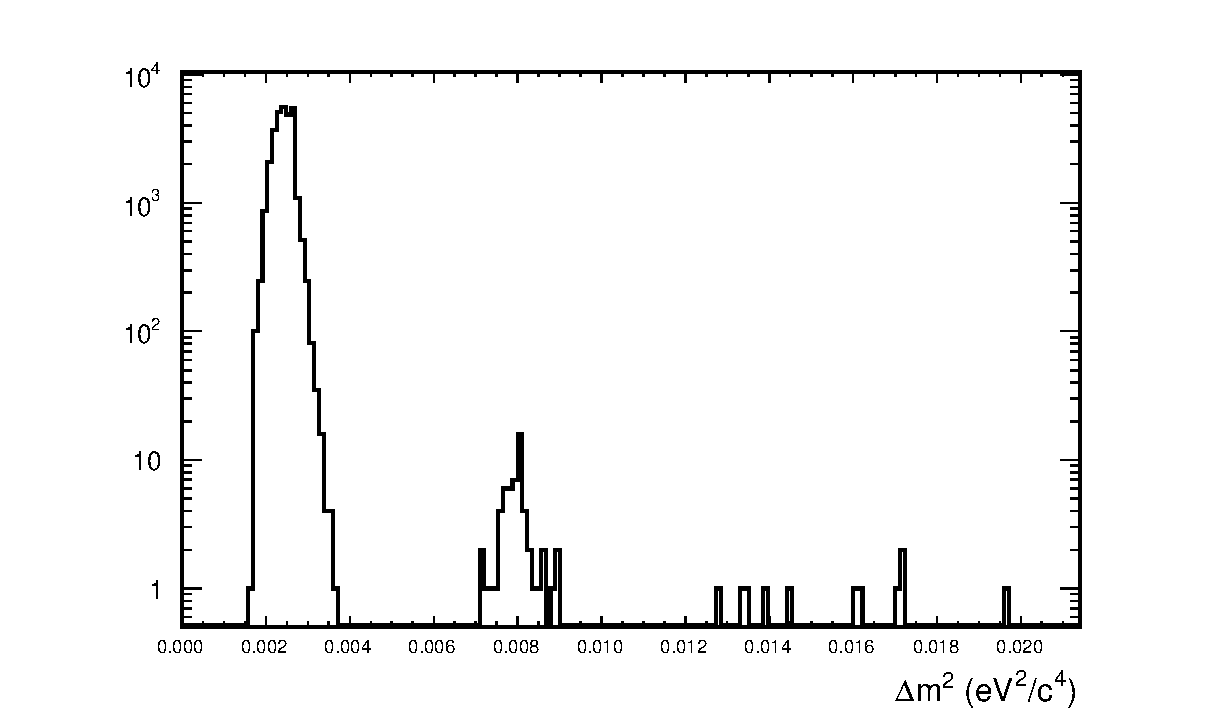
\includegraphics[width=27pc]{./images/etc/dmsq-distribution-2p35Em3-1p0-3x.eps}
\caption{
  Distribution of best-fit $\Delta m^{2}_{23}$ values for a set of toy MC experiments
  generated with the MINOS best-fit values ($\Delta m^{2}_{23}$ = 2.35$\times10^{-3}$ $eV^{2}/c^{4}$
  and maximal mixing). The toy MC experiments were generated for an 
  integrated neutrino beam exposure of $1\times10^{20}$ POT (3 $\times$ 2010a) and systematic variations were included.
  0.2\% of fits gave a $\Delta m^{2}_{23}$ value above 6$\times10^{-3}$ $eV^{2}/c^{4}$.
}
\label{fig:dmsq-distribution-2p35Em3-1p0-3x}
\end{figure*}


%
%
%\section {Alternative hypotheses fits to the $3.23\times10^{19}$ POT dataset}
%\label{sec:altfit_runI}
%
%To be written.
%
%\begin{figure*}[htb]
%\center
%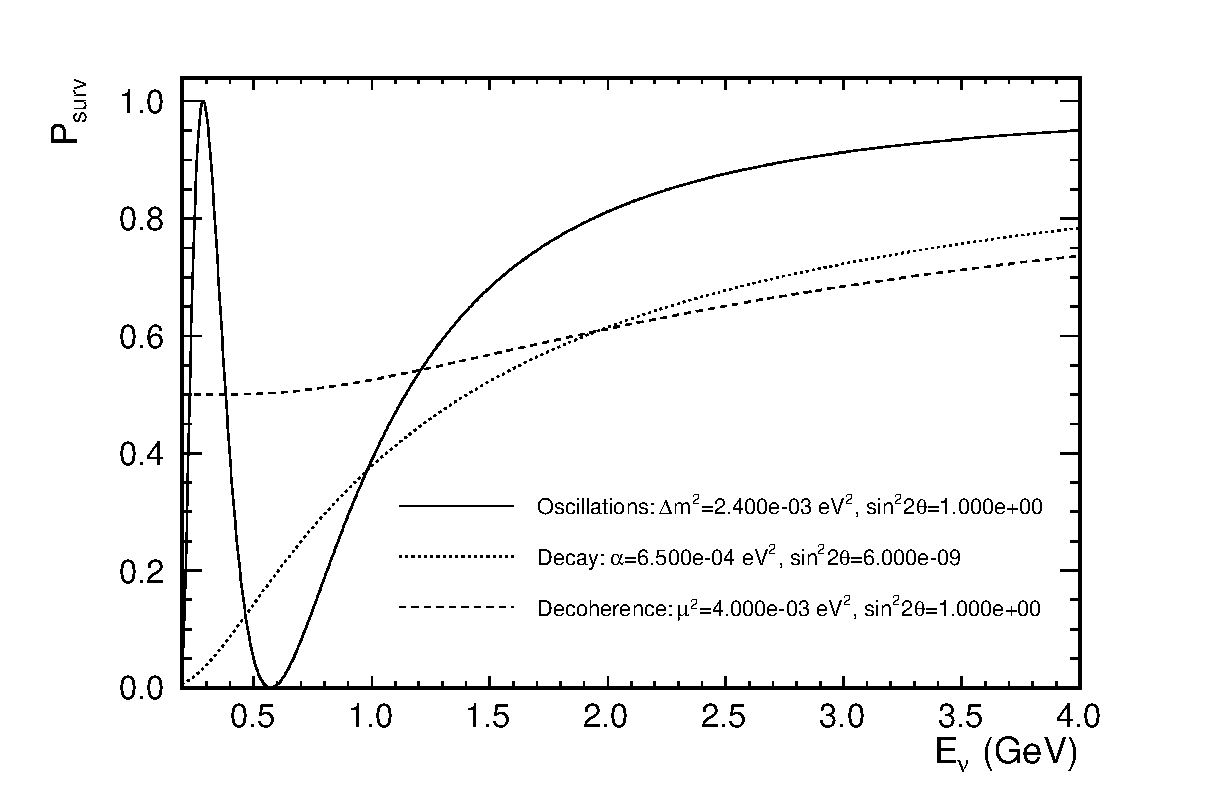
\includegraphics[width=38pc]{./images/etc/psurv_models.eps}
%\caption{
%  Estimated $\nu_{\mu}$ survival probabilities as function of true neutrino energy,
%  under the neutrino oscillation, decay \cite{Decay} and decoherence \cite{Decoherence} hypotheses.
%  Characteristic physics parameters (shown on the plot) were used for each model.
%}
%\label{fig:psurv_models}
%\end{figure*}
%
%

%\section {T2K disappearance analysis prospects (short-term)}
\label{sec:prospects}

To be written.


\section {Future directions of the Rutherford/Oxford analysis}
\label{sec:future}

Over the next few months, 
in preparation for the $\nu_{\mu}$ disappearance analysis using the extended dataset from the November 2010 - June 2011 physics run, 
this analysis will be incrementaly updated using additional inputs from the Rutherford/Oxford/Lancs ND280 analyses 
(CC inclusive reconstructed energy spectrum, measurements of CCQE / CC inclusive and CC1$\pi^{+}$ / CC inclusive, 
measurements of $\pi^{+}$ momentum spectrum in CC1$\pi^{+}$ etc).
The full oscillation analysis will be used to benchmark the utility of each additional ND280 input.

Informed by these studies, we will prepare a document, well in advance of the next global T2K analysis effort,
detailing our views on the optimum methodology for the next $\nu_{\mu}$ disappearance analysis.

\section {Summary}
\label{sec:summary}

To be written.


%
% Appendix
%
\clearpage
\appendix
\addappheadtotoc
\clearpage

\section{Sample mock data fits}

In order for the reader to gain an understanding of the difficulties involved in fitting the reconstructed
energy spectrum from a $3.23 \times 10^{19}$ POT dataset
(just over 6 1-ring $\mu$-like events are expected by both GENIE and NEUT for oscillations with
$sin^{2}2\theta_{23}$ = 1.00 and $\Delta m^{2}_{23}$ = 2.4$\times10^{-3}$ $eV^{2}/c^{4}$),
we present a series of mock-dataset fits (Figs. \ref{fig:mock_data_fit_1} - \ref{fig:mock_data_fit_8}).
The mock-dataset were both generated 
(with true oscillation parameters $sin^{2}2\theta_{23}$ = 1.00 and $\Delta m^{2}_{23}$ = 2.4$\times10^{-3}$ $eV^{2}/c^{4}$)
and fitted using the GENIE p.d.f's.
In each figure, the top-left plot shows the reconstructed energies of the mock-dataset and the best-fit prediction.
The confidence regions shown on the top-right are the 68\% and 90\% CL regions (statistical errors only) 
calculated using the PDG method 
(Sec. \ref{sec:contour_pdg}).
For reference, the MINOS 90\% CL region is also shown (red line).
The best-fit point is shown with a black-star while the input point is indicated by a red circle.
The bottom-left and bottom-right plots show the $\chi^{2}$/ndof along the  $sin^{2}2\theta_{23}$ and $\Delta m^{2}_{23}$
lines that pass through the best-fit point\footnote{
 Note that they {\em are not} marginalized $\chi^{2}$/ndof distributions as functions of $sin^{2}2\theta_{23}$ and $\Delta m^{2}_{23}$.
}.
Finally, in Fig. \ref{fig:mock_data_fits_summary} we show the best-fit point distribution from a set of 5,000 mock-dataset fits.

\begin{figure}[htb]
\center
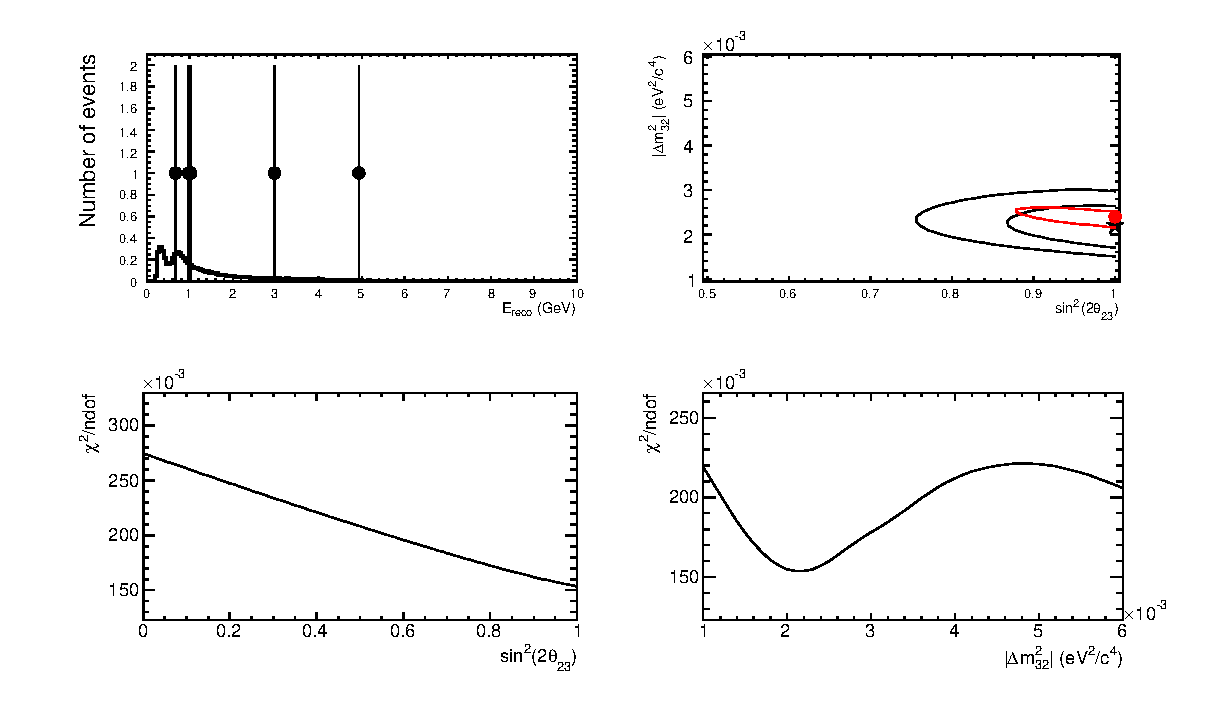
\includegraphics[height=22pc]{./images/fits/mock_sample/mock_fit_1.eps}
\caption{
  Mock-dataset fit 1:
  The reconstructed neutrino energies of the mock 1-ring $\mu$-like data sample
  are \{0.652999, 0.972174, 1.0032, 2.98126, 4.91308\} GeV.
  The best-fit oscillation parameters are 
  $sin^{2}2\theta_{23}$ = 1.00 and $\Delta m^{2}_{23}$ = 2.2$\times10^{-3}$ $eV^{2}/c^{4}$.
}
\label{fig:mock_data_fit_1}
\end{figure}

\begin{figure}[htb]
\center
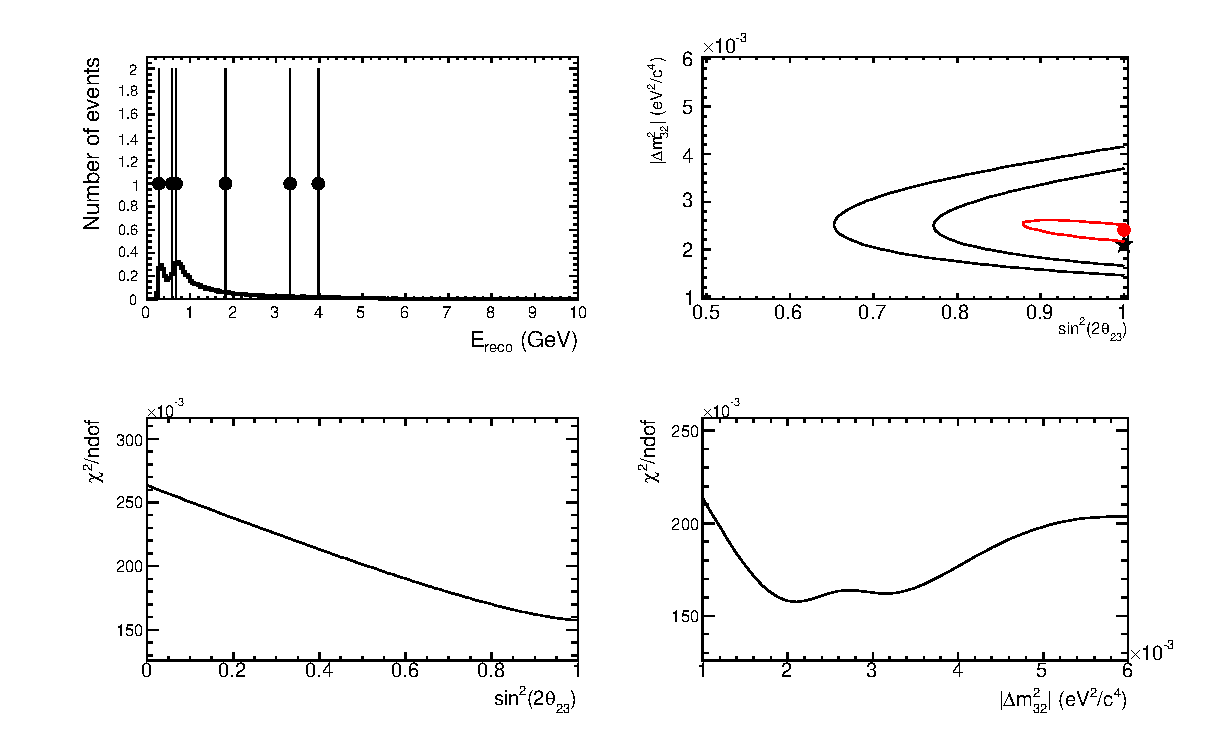
\includegraphics[height=20pc]{./images/fits/mock_sample/mock_fit_2.eps}
\caption{
  Mock-dataset fit 2:
  The reconstructed neutrino energies of the mock 1-ring $\mu$-like data sample
  are \{0.253796, 0.574917, 0.654082, 1.82992, 3.33207, 3.95891\} GeV.
  The best-fit oscillation parameters are 
  $sin^{2}2\theta_{23}$ = 1.00 and $\Delta m^{2}_{23}$ = 2.1$\times10^{-3}$ $eV^{2}/c^{4}$.
}
\label{fig:mock_data_fit_2}
\end{figure}

\begin{figure}[htb]
\center
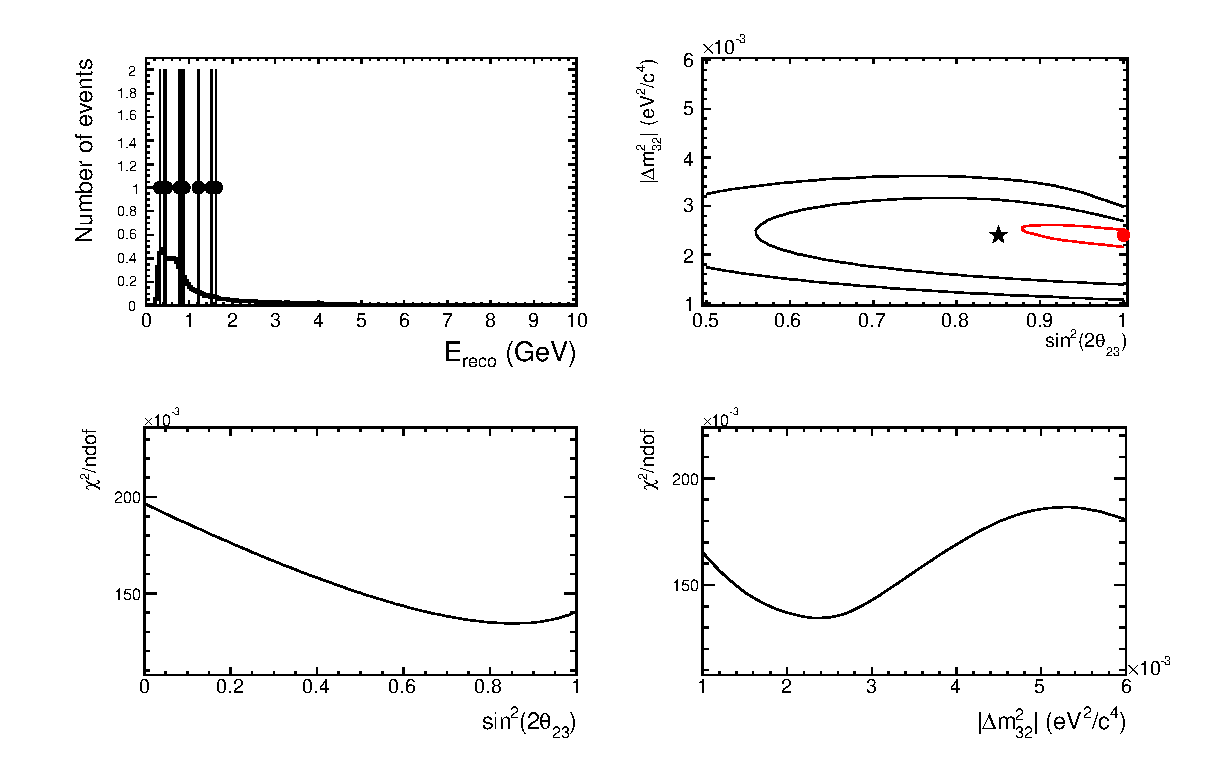
\includegraphics[height=20pc]{./images/fits/mock_sample/mock_fit_3.eps}
\caption{
  Mock-dataset fit 3:
  The reconstructed neutrino energies of the mock 1-ring $\mu$-like data sample
  are \{0.32655, 0.427434, 0.480255, 0.774868, 0.841949, 0.85971, 1.24938, 1.5061, 1.63616\} GeV.
  The best-fit oscillation parameters are 
  $sin^{2}2\theta_{23}$ = 0.85 and $\Delta m^{2}_{23}$ = 2.4$\times10^{-3}$ $eV^{2}/c^{4}$.
}
\label{fig:mock_data_fit_3}
\end{figure}

\begin{figure}[htb]
\center
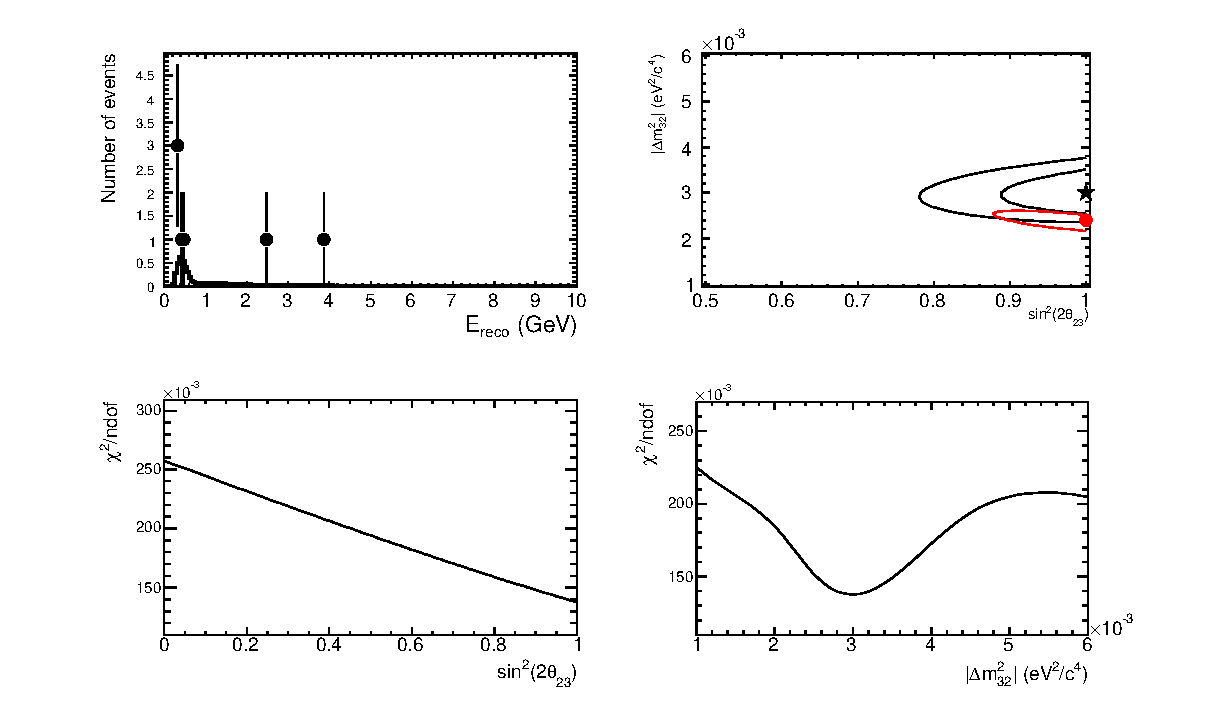
\includegraphics[height=20pc]{./images/fits/mock_sample/mock_fit_4.eps}
\caption{
  Mock-dataset fit 4:
  The reconstructed neutrino energies of the mock 1-ring $\mu$-like data sample
  are \{0.310258, 0.343666, 0.346476, 0.429402, 0.455564, 2.48224, 3.87468\} GeV.
  The best-fit oscillation parameters are 
  $sin^{2}2\theta_{23}$ = 1.00 and $\Delta m^{2}_{23}$ = 3.0$\times10^{-3}$ $eV^{2}/c^{4}$.
}
\label{fig:mock_data_fit_4}
\end{figure}

\begin{figure}[htb]
\center
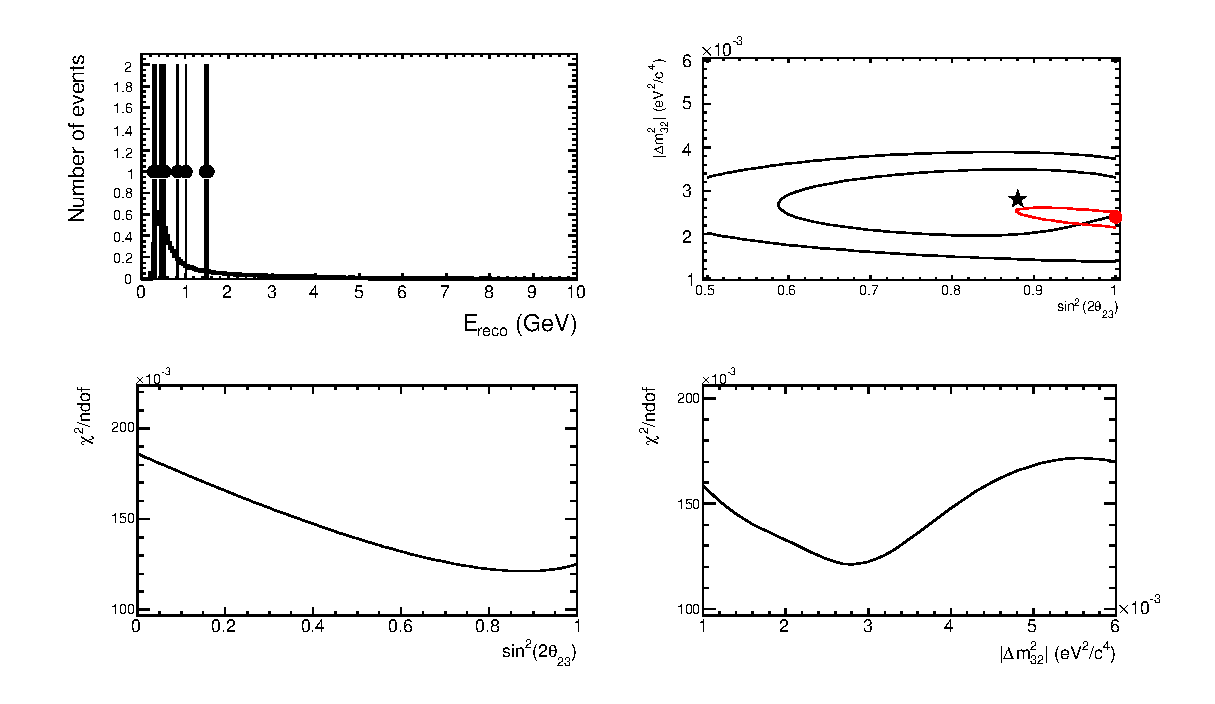
\includegraphics[height=20pc]{./images/fits/mock_sample/mock_fit_5.eps}
\caption{
  Mock-dataset fit 5:
  The reconstructed neutrino energies of the mock 1-ring $\mu$-like data sample
  are \{0.28082, 0.328775, 0.44747, 0.45361, 0.543383, 0.812863, 1.03911, 1.45479, 1.53207\} GeV.
  The best-fit oscillation parameters are 
  $sin^{2}2\theta_{23}$ = 0.88 and $\Delta m^{2}_{23}$ = 2.8$\times10^{-3}$ $eV^{2}/c^{4}$.
}
\label{fig:mock_data_fit_5}
\end{figure}

\begin{figure}[htb]
\center
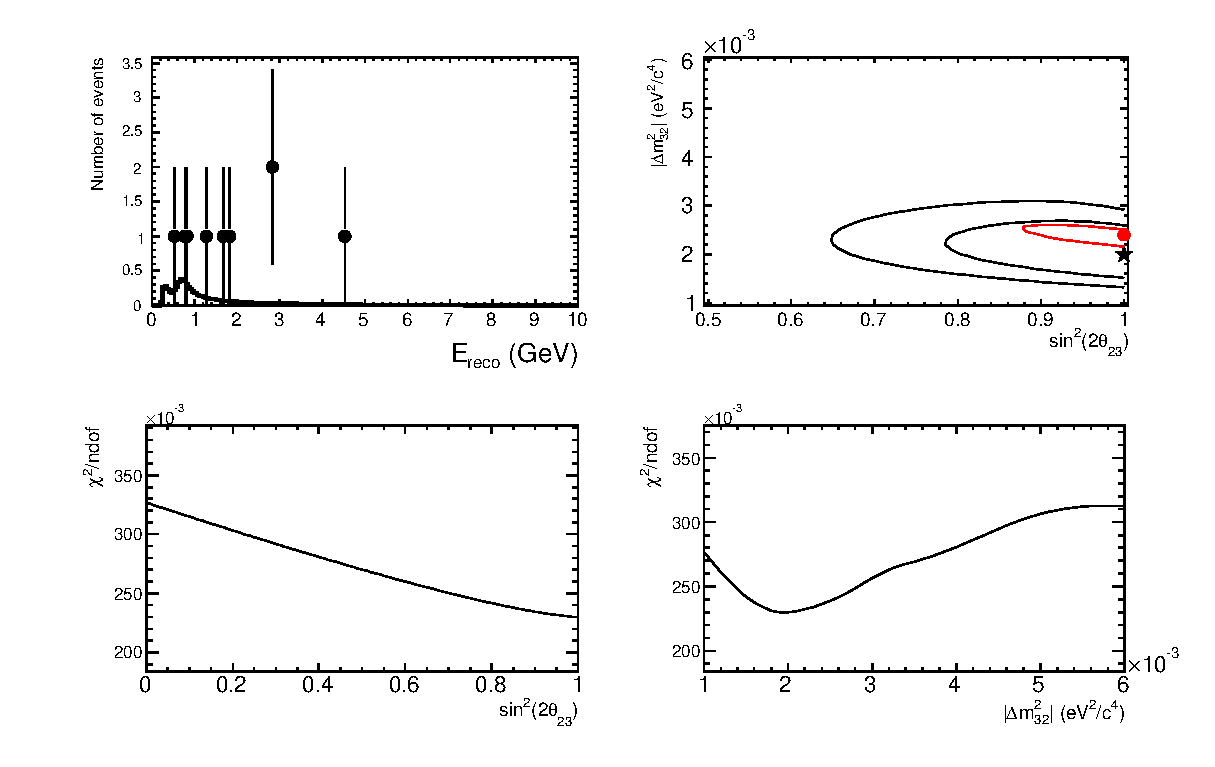
\includegraphics[height=20pc]{./images/fits/mock_sample/mock_fit_6.eps}
\caption{
  Mock-dataset fit 6:
  The reconstructed neutrino energies of the mock 1-ring $\mu$-like data sample
  are \{0.540056, 0.771411, 0.815833, 1.27384, 1.69788, 1.8422, 2.84393, 2.8057, 4.5466\} GeV.
  The best-fit oscillation parameters are 
  $sin^{2}2\theta_{23}$ = 1.00 and $\Delta m^{2}_{23}$ = 2.0$\times10^{-3}$ $eV^{2}/c^{4}$.
}
\label{fig:mock_data_fit_6}
\end{figure}

\begin{figure}[htb]
\center
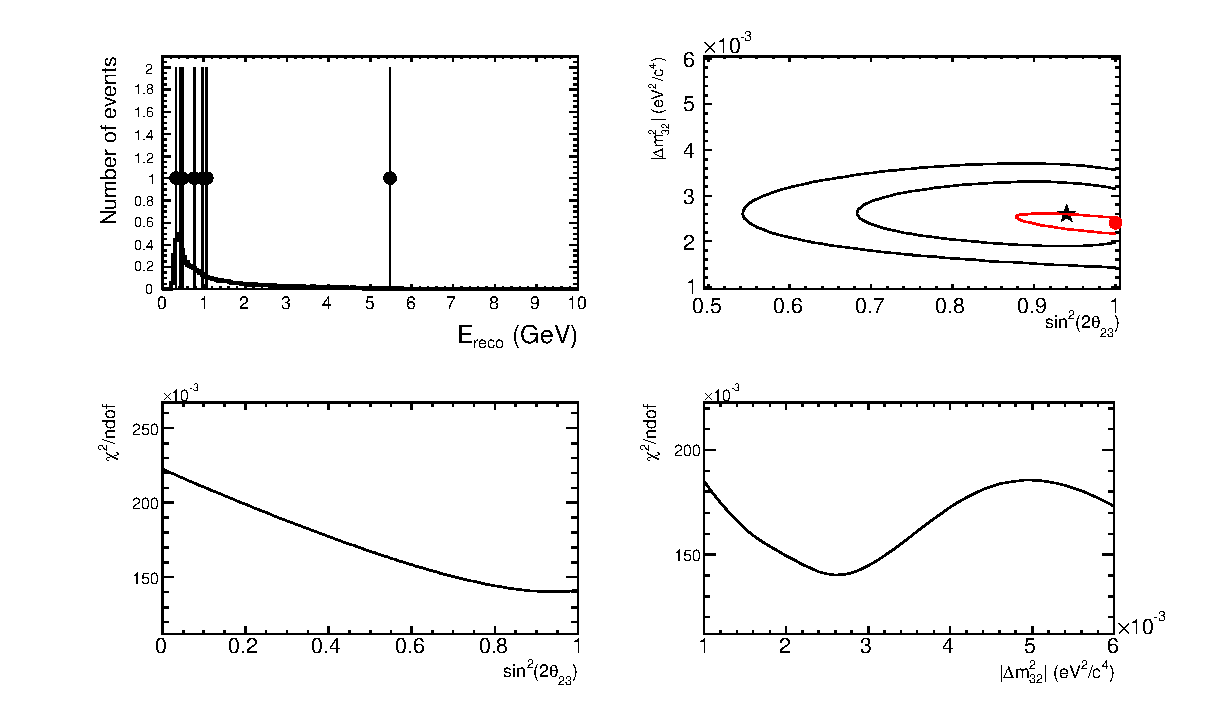
\includegraphics[height=20pc]{./images/fits/mock_sample/mock_fit_7.eps}
\caption{
  Mock-dataset fit 7:
  The reconstructed neutrino energies of the mock 1-ring $\mu$-like data sample
  are \{0.319674, 0.407844, 0.462414, 0.759538, 0.968712, 1.06938, 5.4639\} GeV.
  The best-fit oscillation parameters are 
  $sin^{2}2\theta_{23}$ = 0.94 and $\Delta m^{2}_{23}$ = 2.6$\times10^{-3}$ $eV^{2}/c^{4}$.
}
\label{fig:mock_data_fit_7}
\end{figure}

\begin{figure}[htb]
\center
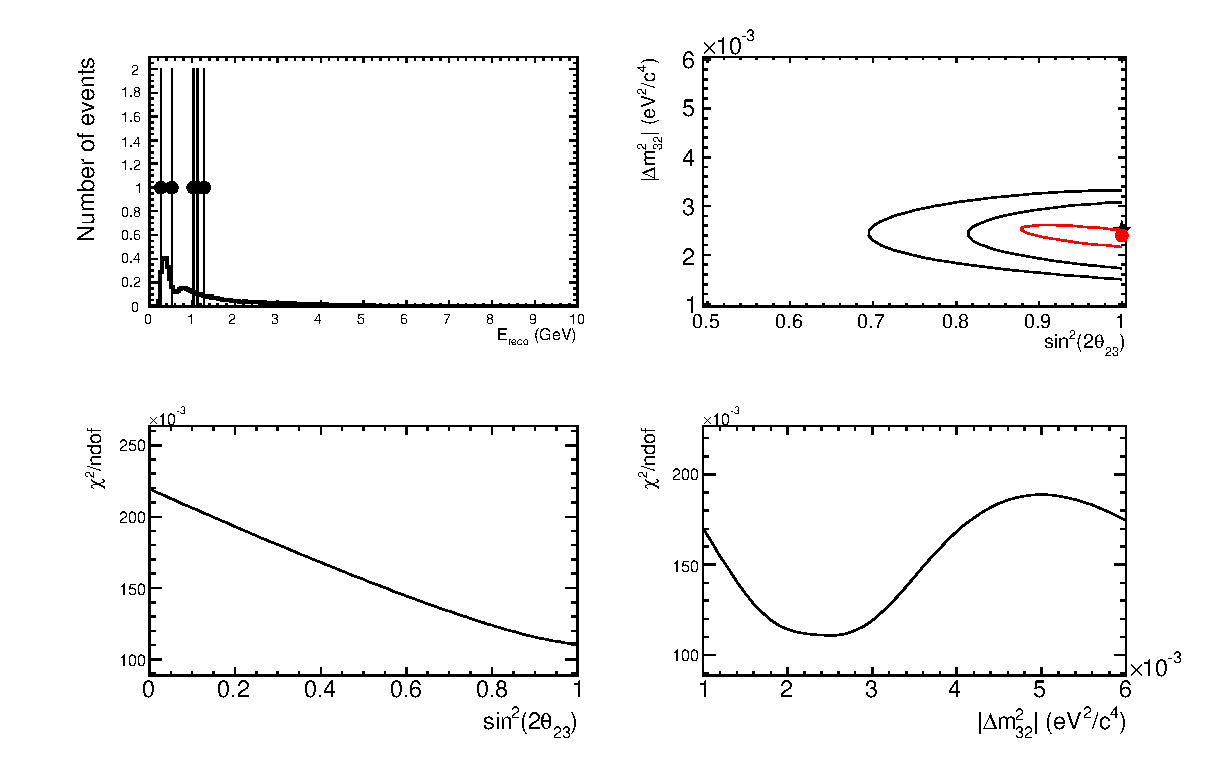
\includegraphics[height=20pc]{./images/fits/mock_sample/mock_fit_8.eps}
\caption{
  Mock-dataset fit 8:
  The reconstructed neutrino energies of the mock 1-ring $\mu$-like data sample
  are \{0.264395, 0.530563, 1.01775, 1.12194, 1.28155\} GeV.
  The best-fit oscillation parameters are 
  $sin^{2}2\theta_{23}$ = 1.00 and $\Delta m^{2}_{23}$ = 2.5$\times10^{-3}$ $eV^{2}/c^{4}$.
}
\label{fig:mock_data_fit_8}
\end{figure}

\begin{figure}[htb]
\center
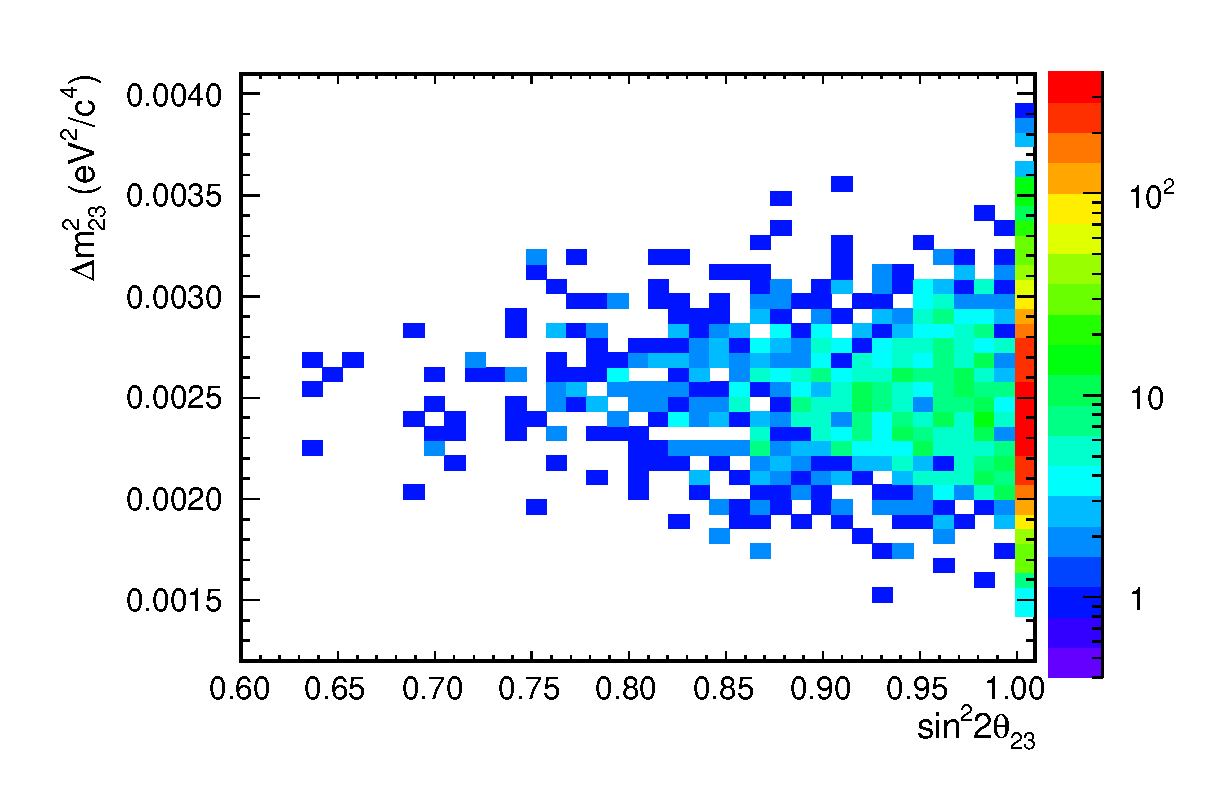
\includegraphics[height=20pc]{./images/fits/mock_sample/bestpoints_5k_mockfits.eps}
\caption{
  Distribution of best-fit oscillation parameters for 5,000 mock-dataset fits.
}
\label{fig:mock_data_fits_summary}
\end{figure}

\clearpage
\clearpage

\section{Effect of systematic parameters on predicted SuperK energy spectrum}
\label{appendix:effect_of_systematics}

%
% SuperK CCQE efficiency
%

\begin{figure}[ht]
\begin{minipage}[t]{0.47\linewidth}
\centering
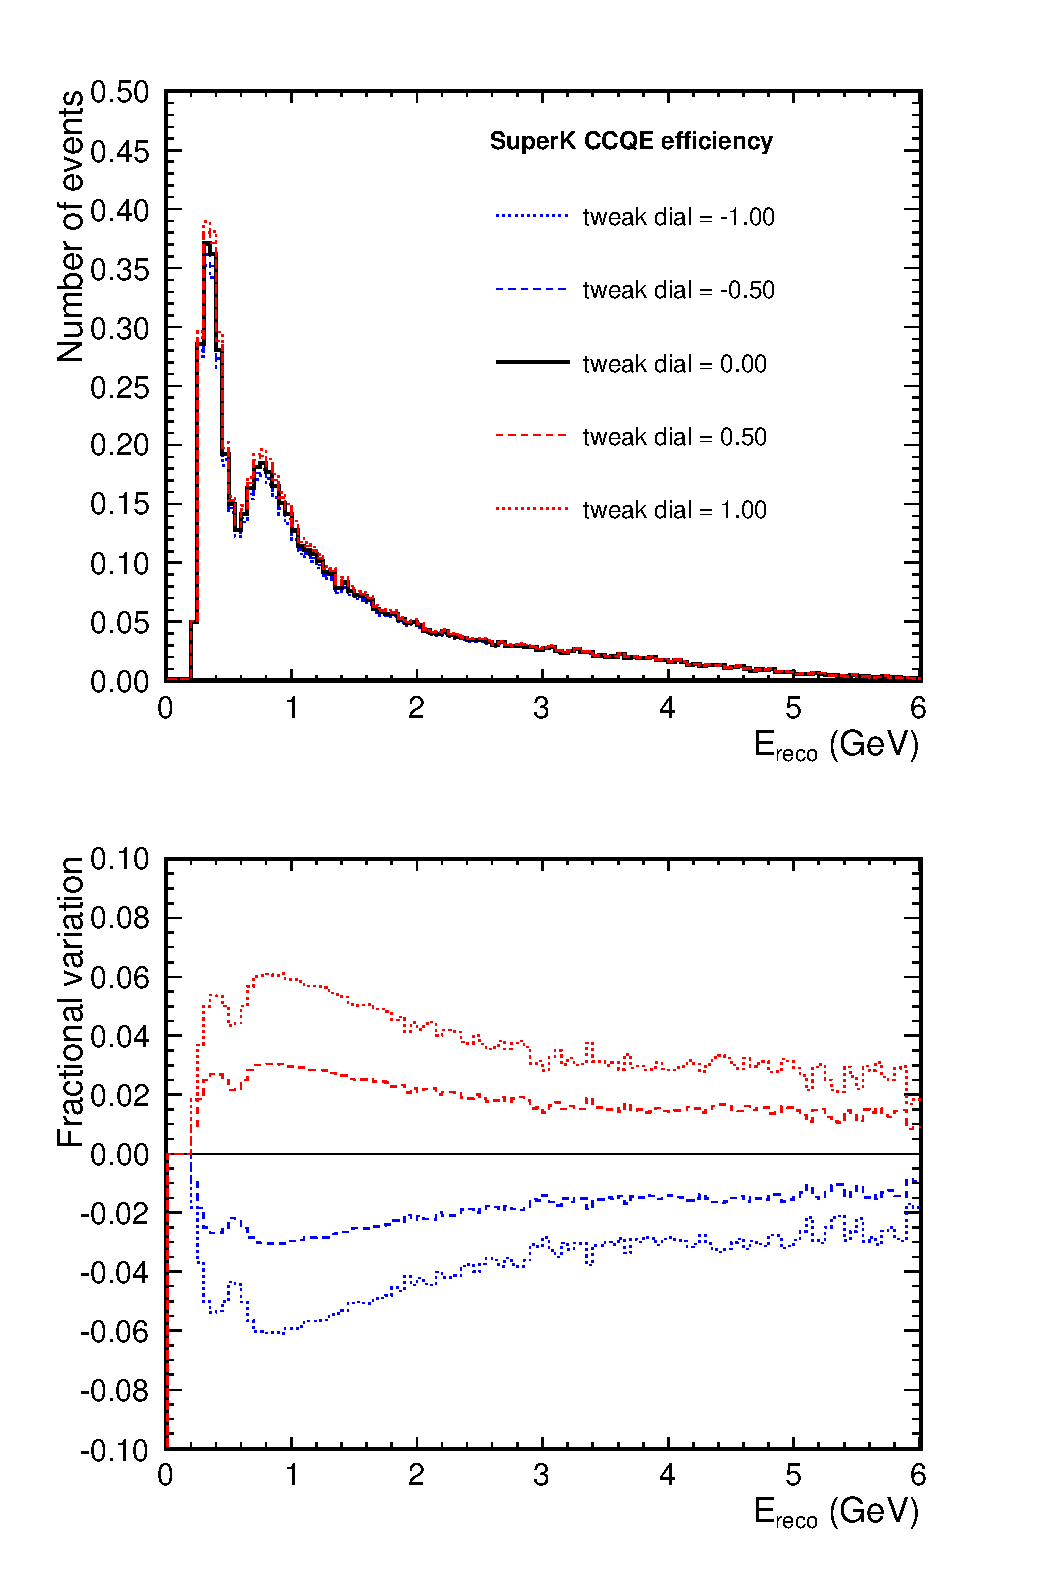
\includegraphics[width=19pc,height=21pc]{./images/predicted_spectrum/systematic_variations/genie_sk_spectrum_twk_skccqeeff_2p4Em3_1p0.eps}
\caption{
  Effect of SuperK CCQE efficiency variation to the GENIE
  reconstructed-energy spectrum of 1-ring muon-like events (after extrapolation).
  All spectra have oscillations with $sin^{2}2\theta_{23}$ = 1.0 and $\Delta m^{2}_{23}$ = 2.4$\times10^{-3}$ $eV^{2}/c^{4}$ applied.  
}
\label{fig:genie_sk_spectrum_twk_skccqeeff_2p4Em3_1p0}
\end{minipage}
\hspace{0.06\linewidth}
\begin{minipage}[t]{0.47\linewidth}
\centering
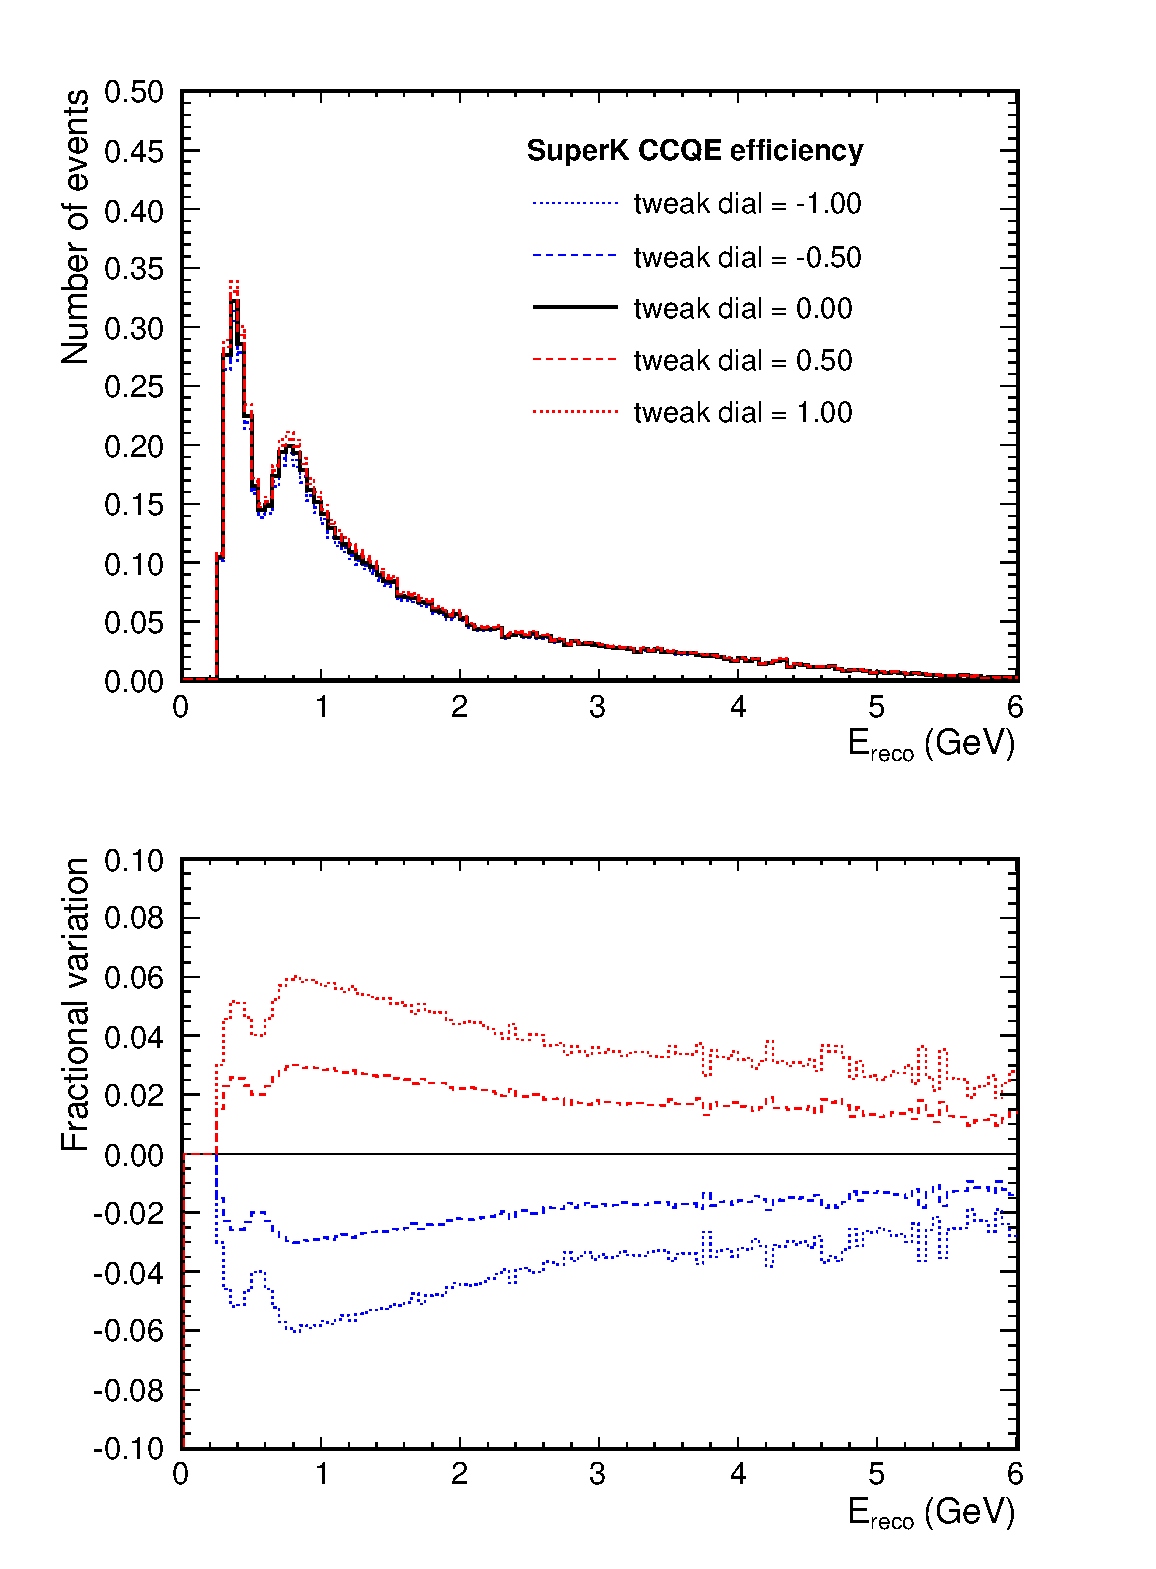
\includegraphics[width=19pc,height=21pc]{images/predicted_spectrum/systematic_variations/neut_sk_spectrum_twk_skccqeeff_2p4Em3_1p0.eps}
\caption{
  Effect of SuperK CCQE efficiency variation to the NEUT
  reconstructed-energy spectrum of 1-ring muon-like events (after extrapolation).
  All spectra have oscillations with $sin^{2}2\theta_{23}$ = 1.0 and $\Delta m^{2}_{23}$ = 2.4$\times10^{-3}$ $eV^{2}/c^{4}$ applied.  
}
\label{fig:neut_sk_spectrum_twk_skccqeeff_2p4Em3_1p0}
\end{minipage}
\end{figure}


%
% SuperK CCnonQE efficiency
%

\begin{figure}[ht]
\begin{minipage}[t]{0.47\linewidth}
\centering
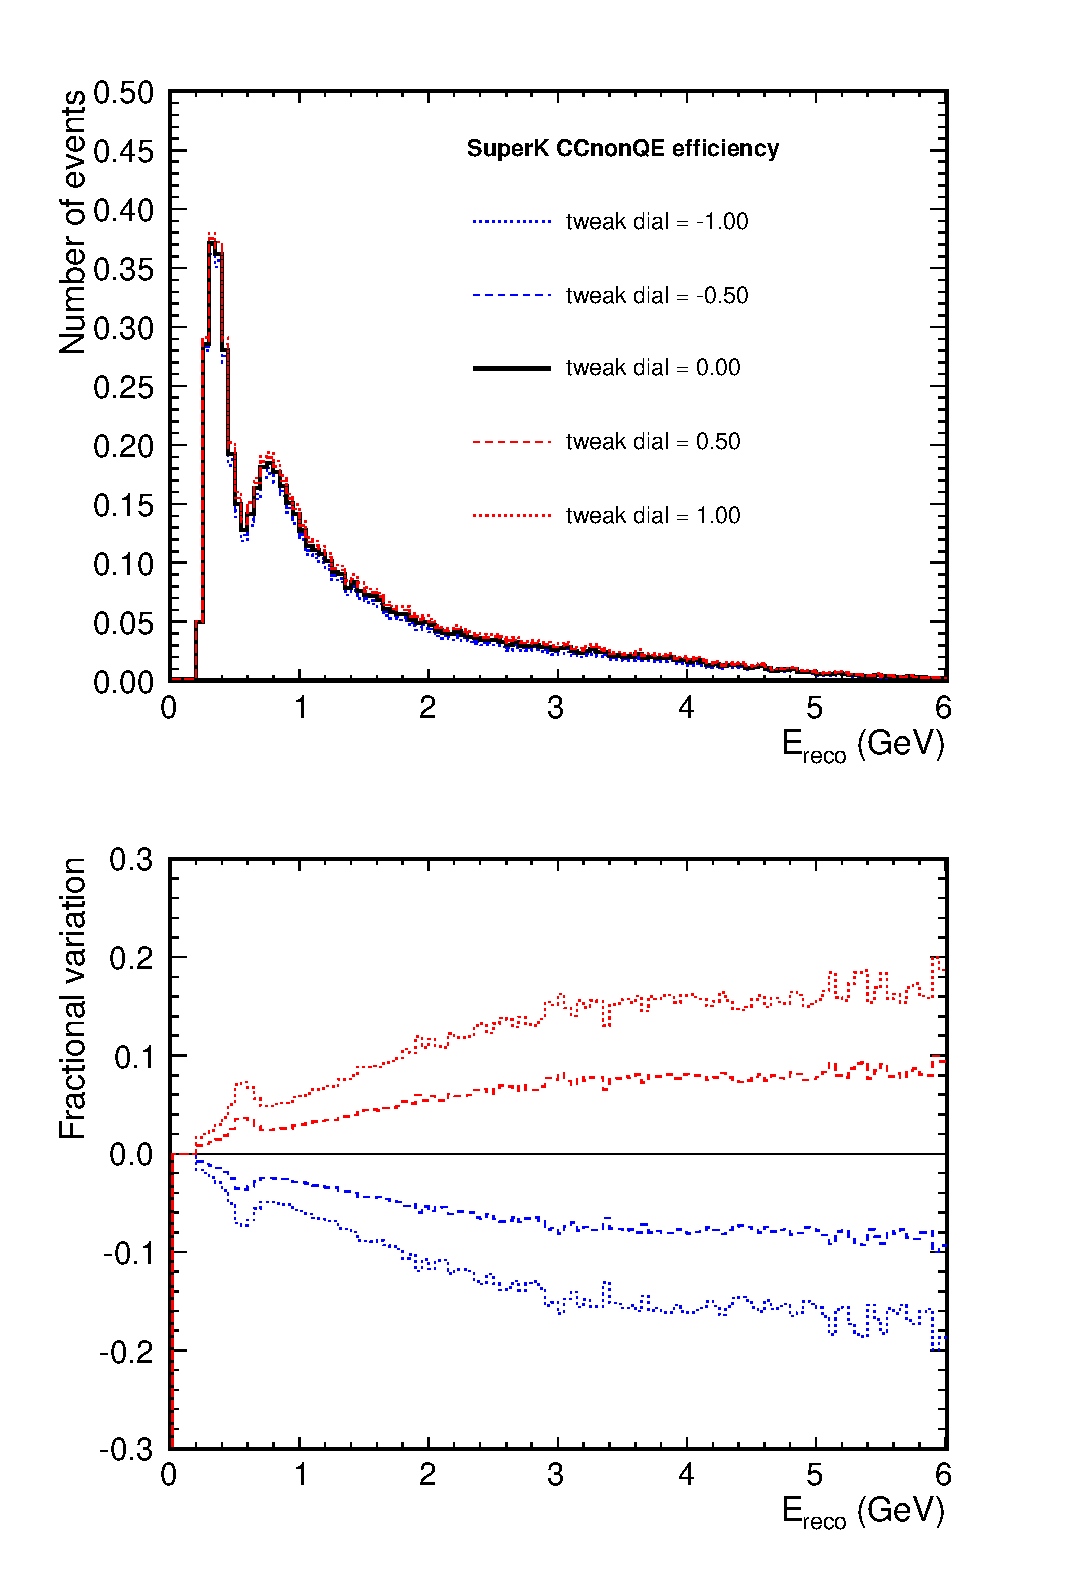
\includegraphics[width=19pc,height=21pc]{./images/predicted_spectrum/systematic_variations/genie_sk_spectrum_twk_skccnonqeeff_2p4Em3_1p0.eps}
\caption{
  Effect of SuperK CCnonQE efficiency variation to the GENIE
  reconstructed-energy spectrum of 1-ring muon-like events (after extrapolation).
  All spectra have oscillations with $sin^{2}2\theta_{23}$ = 1.0 and $\Delta m^{2}_{23}$ = 2.4$\times10^{-3}$ $eV^{2}/c^{4}$ applied.  
}
\label{fig:genie_sk_spectrum_twk_sknonccqeeff_2p4Em3_1p0}
\end{minipage}
\hspace{0.06\linewidth}
\begin{minipage}[t]{0.47\linewidth}
\centering
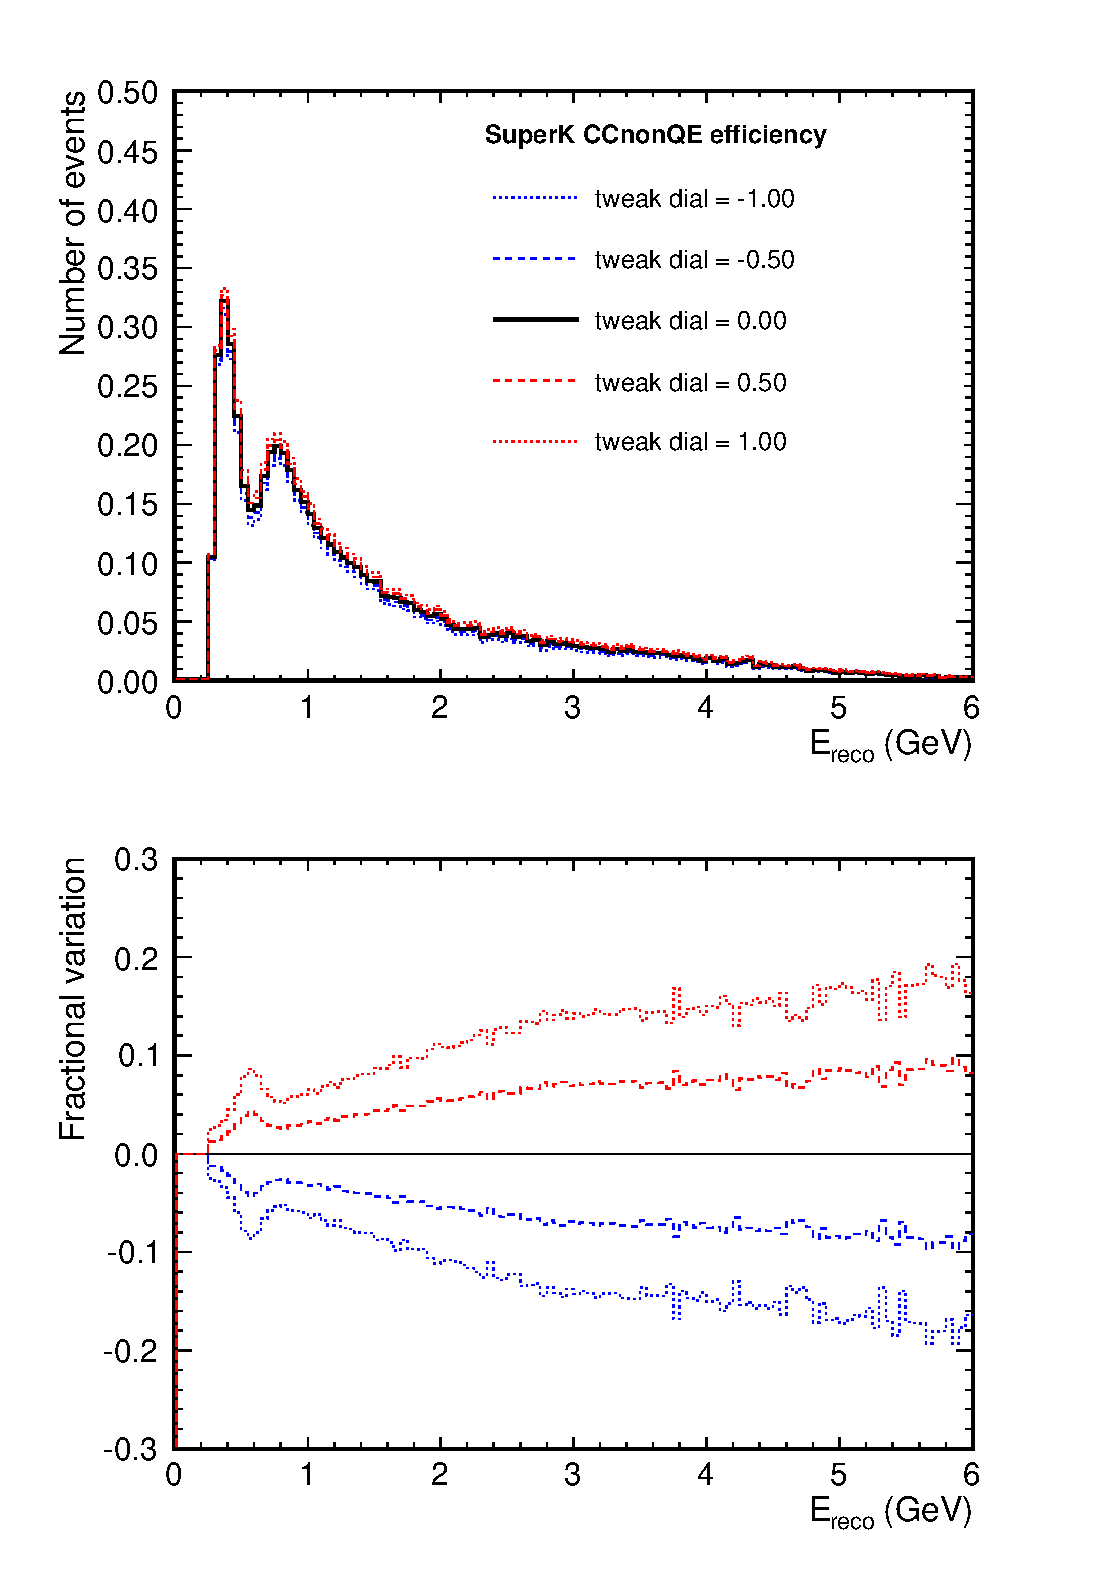
\includegraphics[width=19pc,height=21pc]{images/predicted_spectrum/systematic_variations/neut_sk_spectrum_twk_skccnonqeeff_2p4Em3_1p0.eps}
\caption{
  Effect of SuperK CCnonQE efficiency variation to the NEUT
  reconstructed-energy spectrum of 1-ring muon-like events (after extrapolation).
  All spectra have oscillations with $sin^{2}2\theta_{23}$ = 1.0 and $\Delta m^{2}_{23}$ = 2.4$\times10^{-3}$ $eV^{2}/c^{4}$ applied.  
}
\label{fig:neut_sk_spectrum_twk_skccnonqeeff_2p4Em3_1p0}
\end{minipage}
\end{figure}

%
% SuperK NC efficiency
%

\begin{figure}[ht]
\begin{minipage}[t]{0.47\linewidth}
\centering
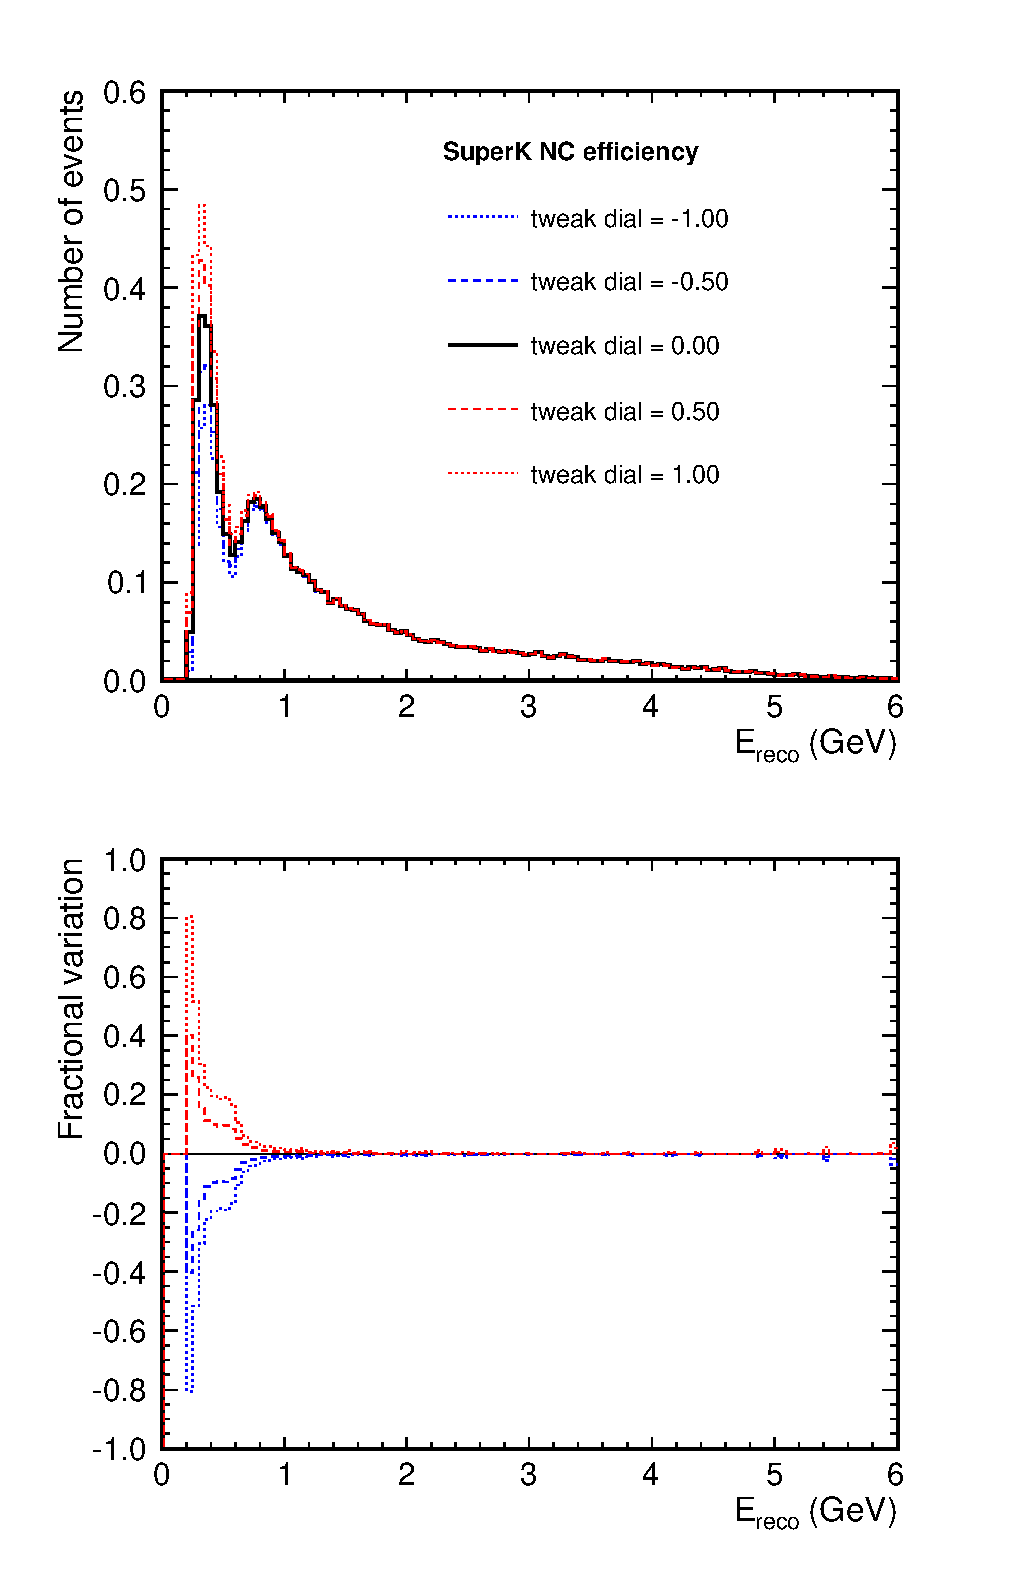
\includegraphics[width=19pc,height=21pc]{./images/predicted_spectrum/systematic_variations/genie_sk_spectrum_twk_sknceff_2p4Em3_1p0.eps}
\caption{
  Effect of SuperK NC efficiency variation to the GENIE
  reconstructed-energy spectrum of 1-ring muon-like events (after extrapolation).
  All spectra have oscillations with $sin^{2}2\theta_{23}$ = 1.0 and $\Delta m^{2}_{23}$ = 2.4$\times10^{-3}$ $eV^{2}/c^{4}$ applied.  
}
\label{fig:genie_sk_spectrum_twk_sknceff_2p4Em3_1p0}
\end{minipage}
\hspace{0.06\linewidth}
\begin{minipage}[t]{0.47\linewidth}
\centering
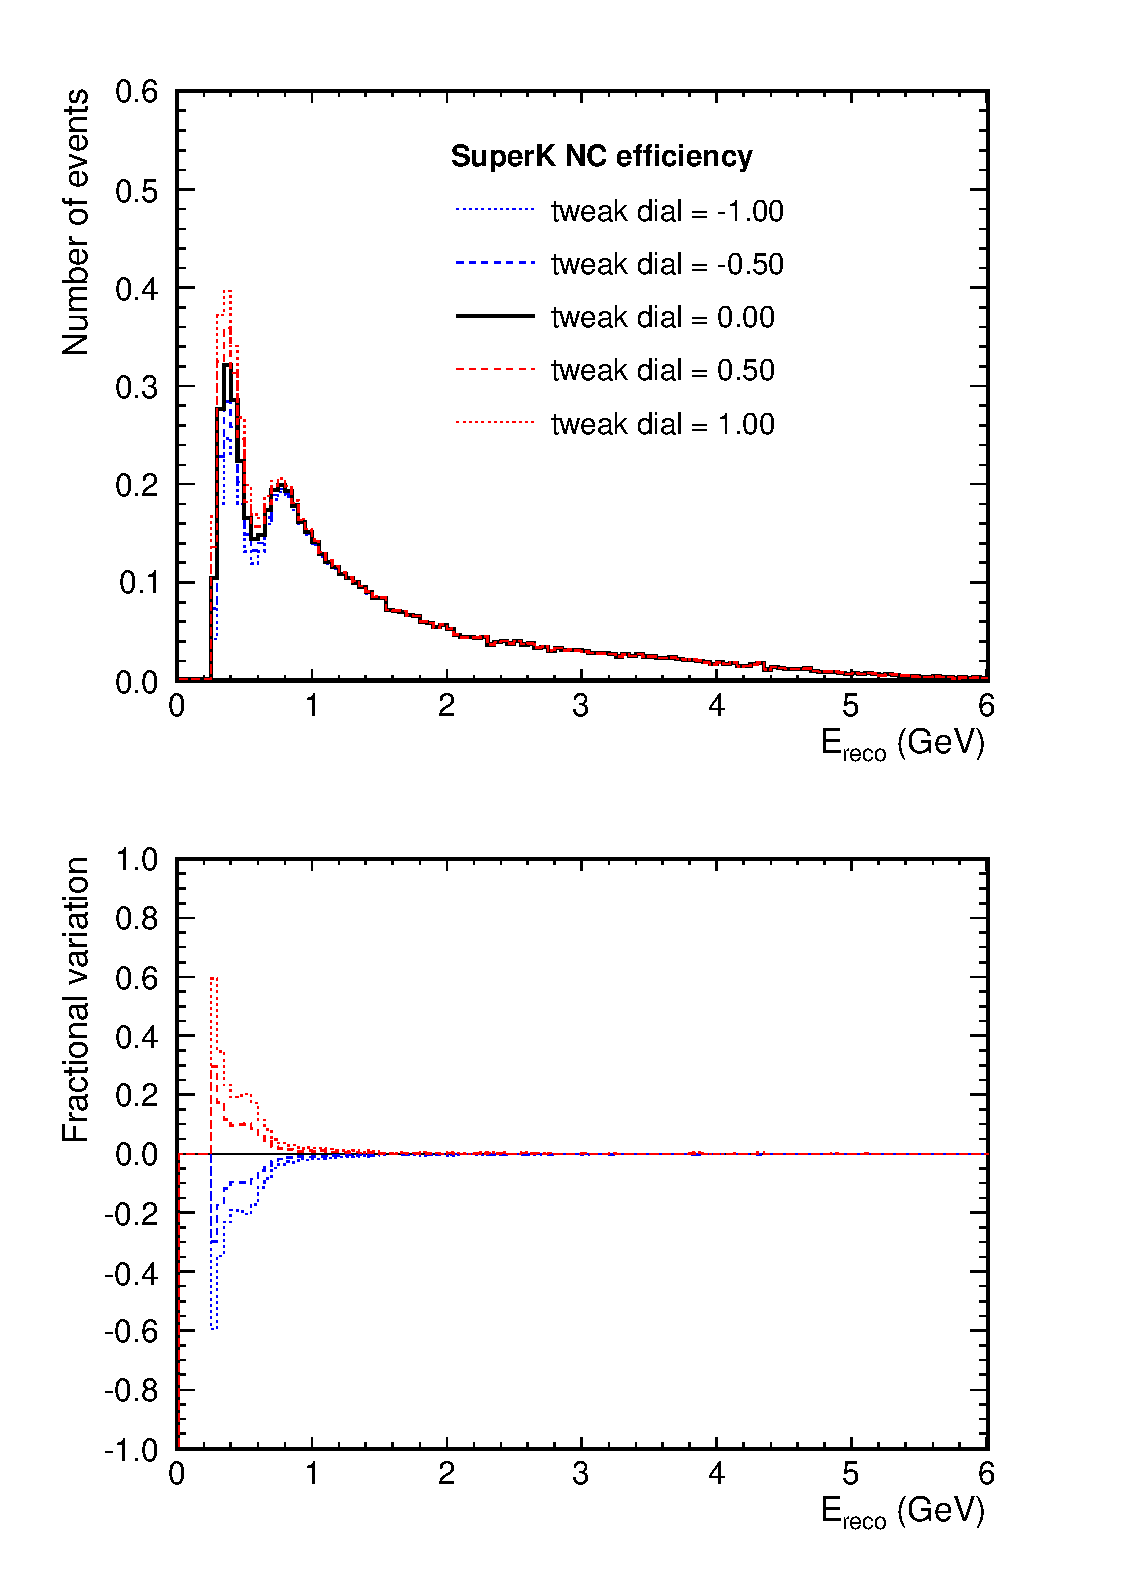
\includegraphics[width=19pc,height=21pc]{images/predicted_spectrum/systematic_variations/neut_sk_spectrum_twk_sknceff_2p4Em3_1p0.eps}
\caption{
  Effect of SuperK NC efficiency variation to the NEUT
  reconstructed-energy spectrum of 1-ring muon-like events (after extrapolation).
  All spectra have oscillations with $sin^{2}2\theta_{23}$ = 1.0 and $\Delta m^{2}_{23}$ = 2.4$\times10^{-3}$ $eV^{2}/c^{4}$ applied.  
}
\label{fig:neut_sk_spectrum_twk_sknceff_2p4Em3_1p0}
\end{minipage}
\end{figure}


%
% SuperK nue CC efficiency
%

\begin{figure}[ht]
\begin{minipage}[t]{0.47\linewidth}
\centering
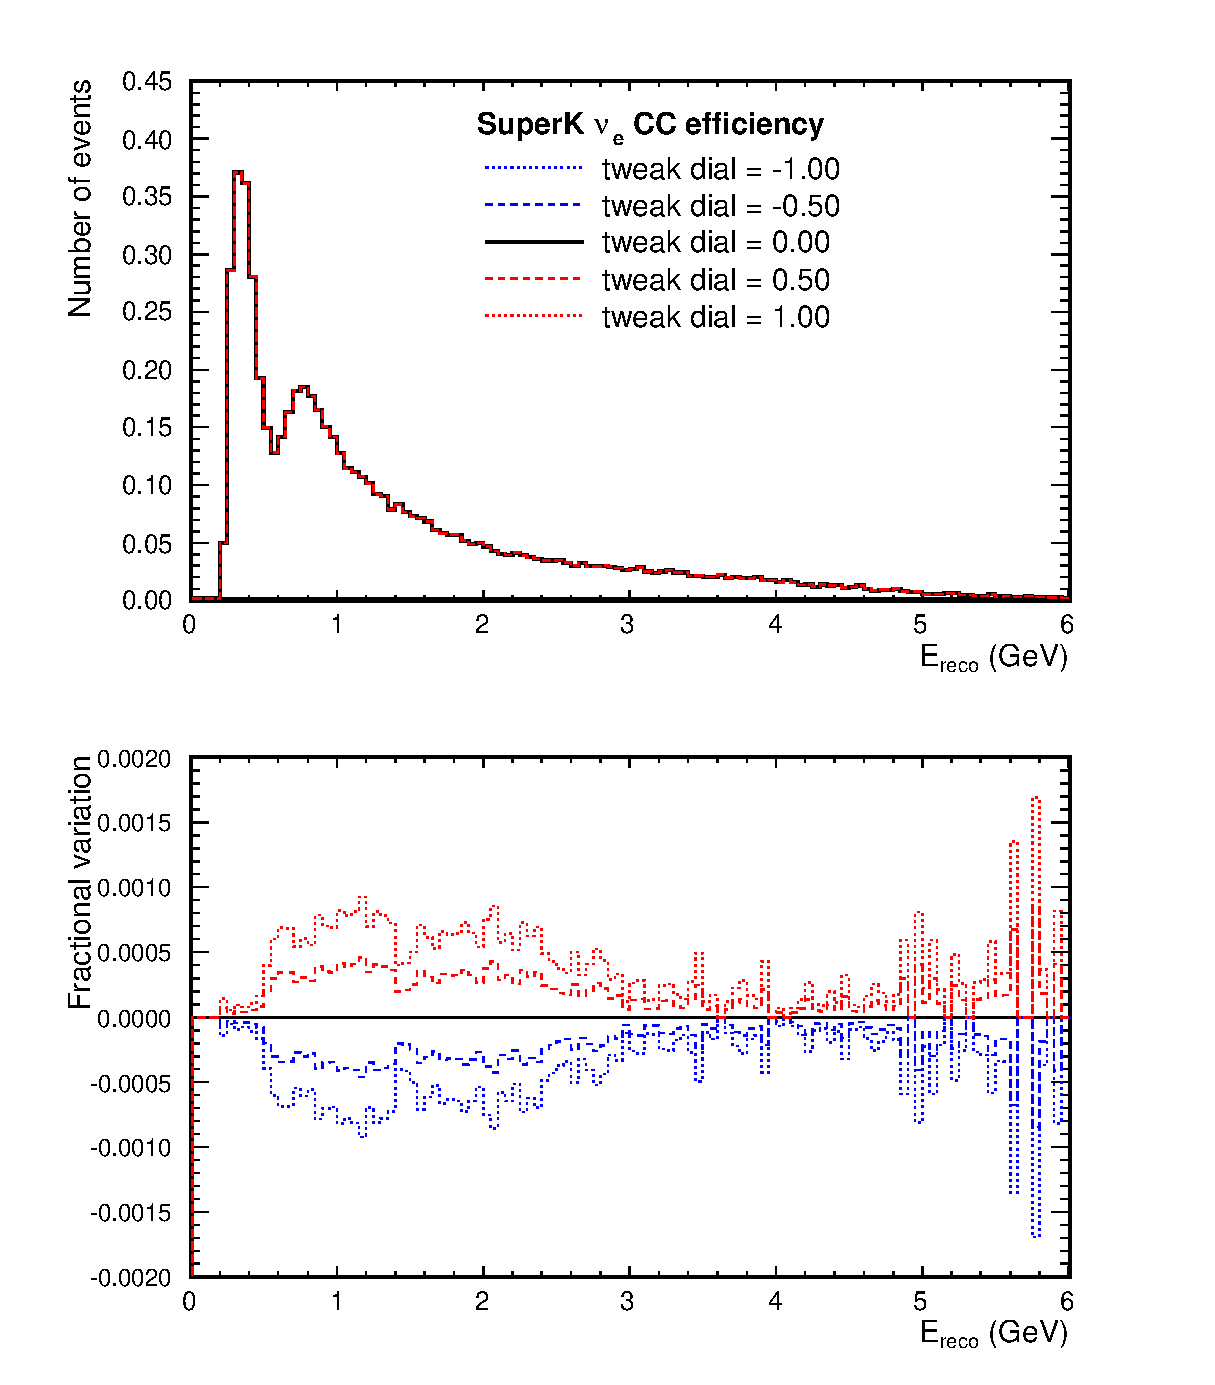
\includegraphics[width=19pc,height=21pc]{./images/predicted_spectrum/systematic_variations/genie_sk_spectrum_twk_sknuecceff_2p4Em3_1p0.eps}
\caption{
  Effect of SuperK $\nu_{e}$ CC efficiency variation to the GENIE
  reconstructed-energy spectrum of 1-ring muon-like events (after extrapolation).
  All spectra have oscillations with $sin^{2}2\theta_{23}$ = 1.0 and $\Delta m^{2}_{23}$ = 2.4$\times10^{-3}$ $eV^{2}/c^{4}$ applied.  
}
\label{fig:genie_sk_spectrum_twk_sknuecceff_2p4Em3_1p0}
\end{minipage}
\hspace{0.06\linewidth}
\begin{minipage}[t]{0.47\linewidth}
\centering
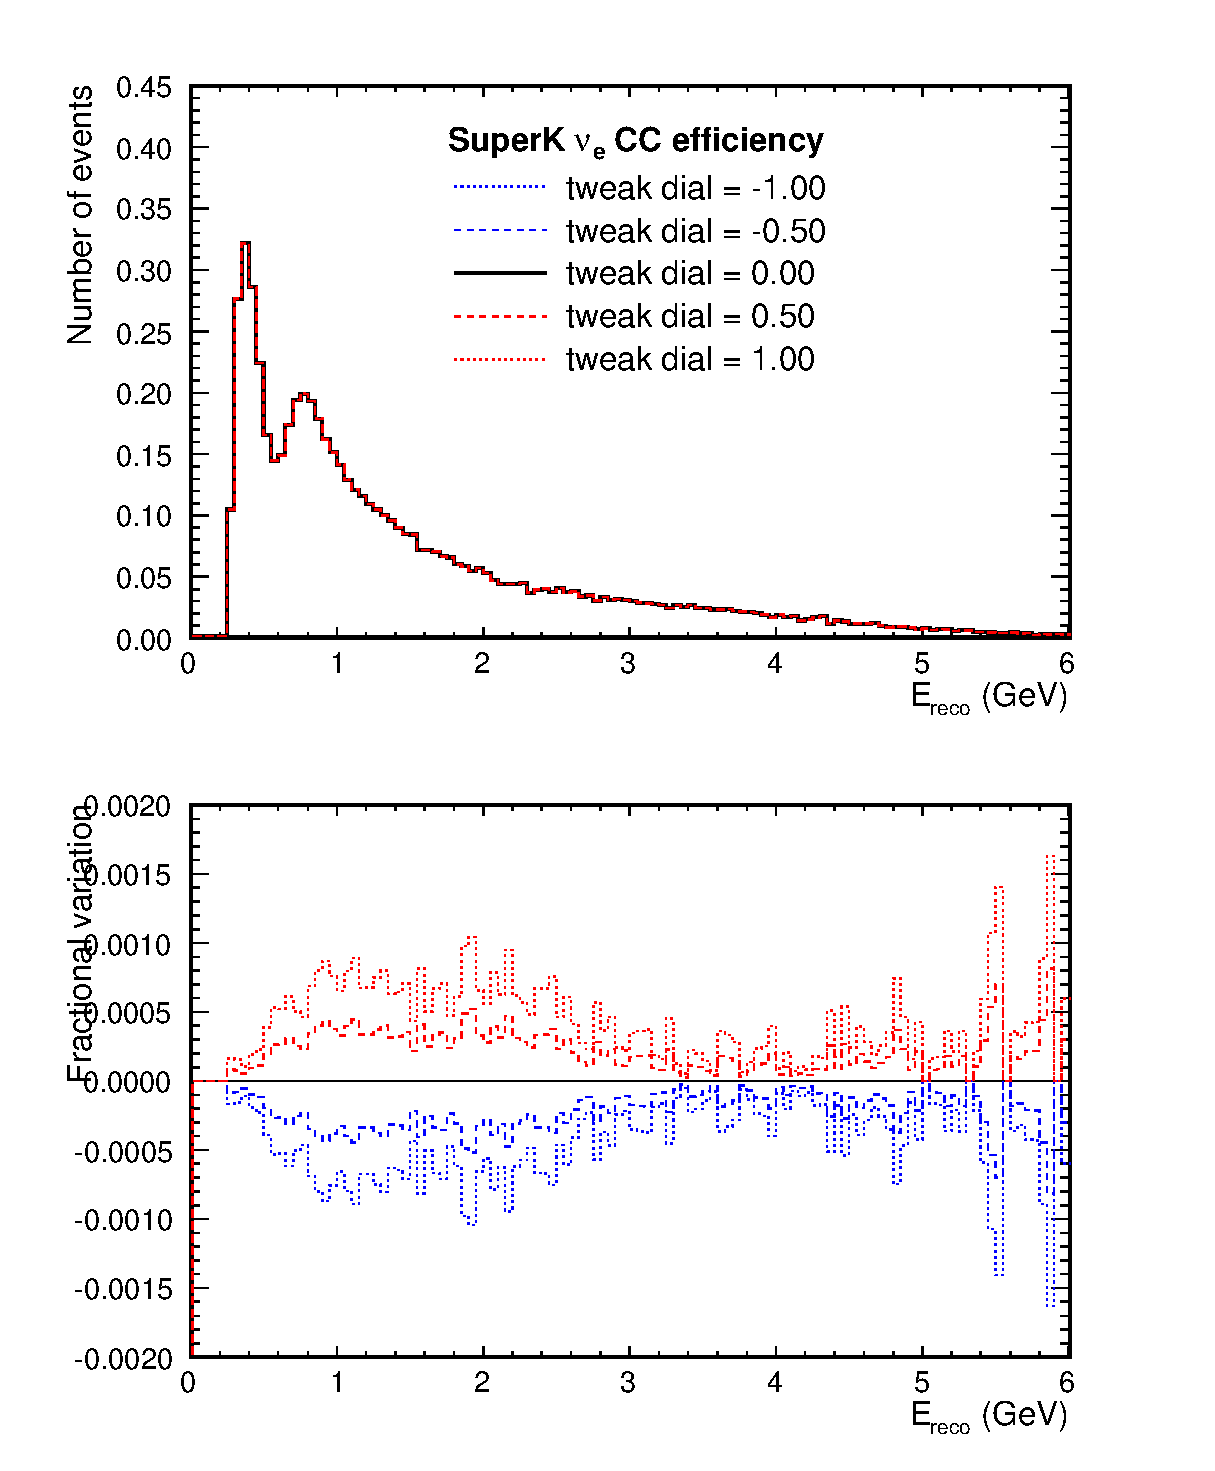
\includegraphics[width=19pc,height=21pc]{images/predicted_spectrum/systematic_variations/neut_sk_spectrum_twk_sknuecceff_2p4Em3_1p0.eps}
\caption{
  Effect of SuperK $\nu_{e}$ CC efficiency variation to the NEUT
  reconstructed-energy spectrum of 1-ring muon-like events (after extrapolation).
  All spectra have oscillations with $sin^{2}2\theta_{23}$ = 1.0 and $\Delta m^{2}_{23}$ = 2.4$\times10^{-3}$ $eV^{2}/c^{4}$ applied.  
}
\label{fig:neut_sk_spectrum_twk_sknuecceff_2p4Em3_1p0}
\end{minipage}
\end{figure}


%
% SuperK energy scale
%

\begin{figure}[ht]
\begin{minipage}[t]{0.47\linewidth}
\centering
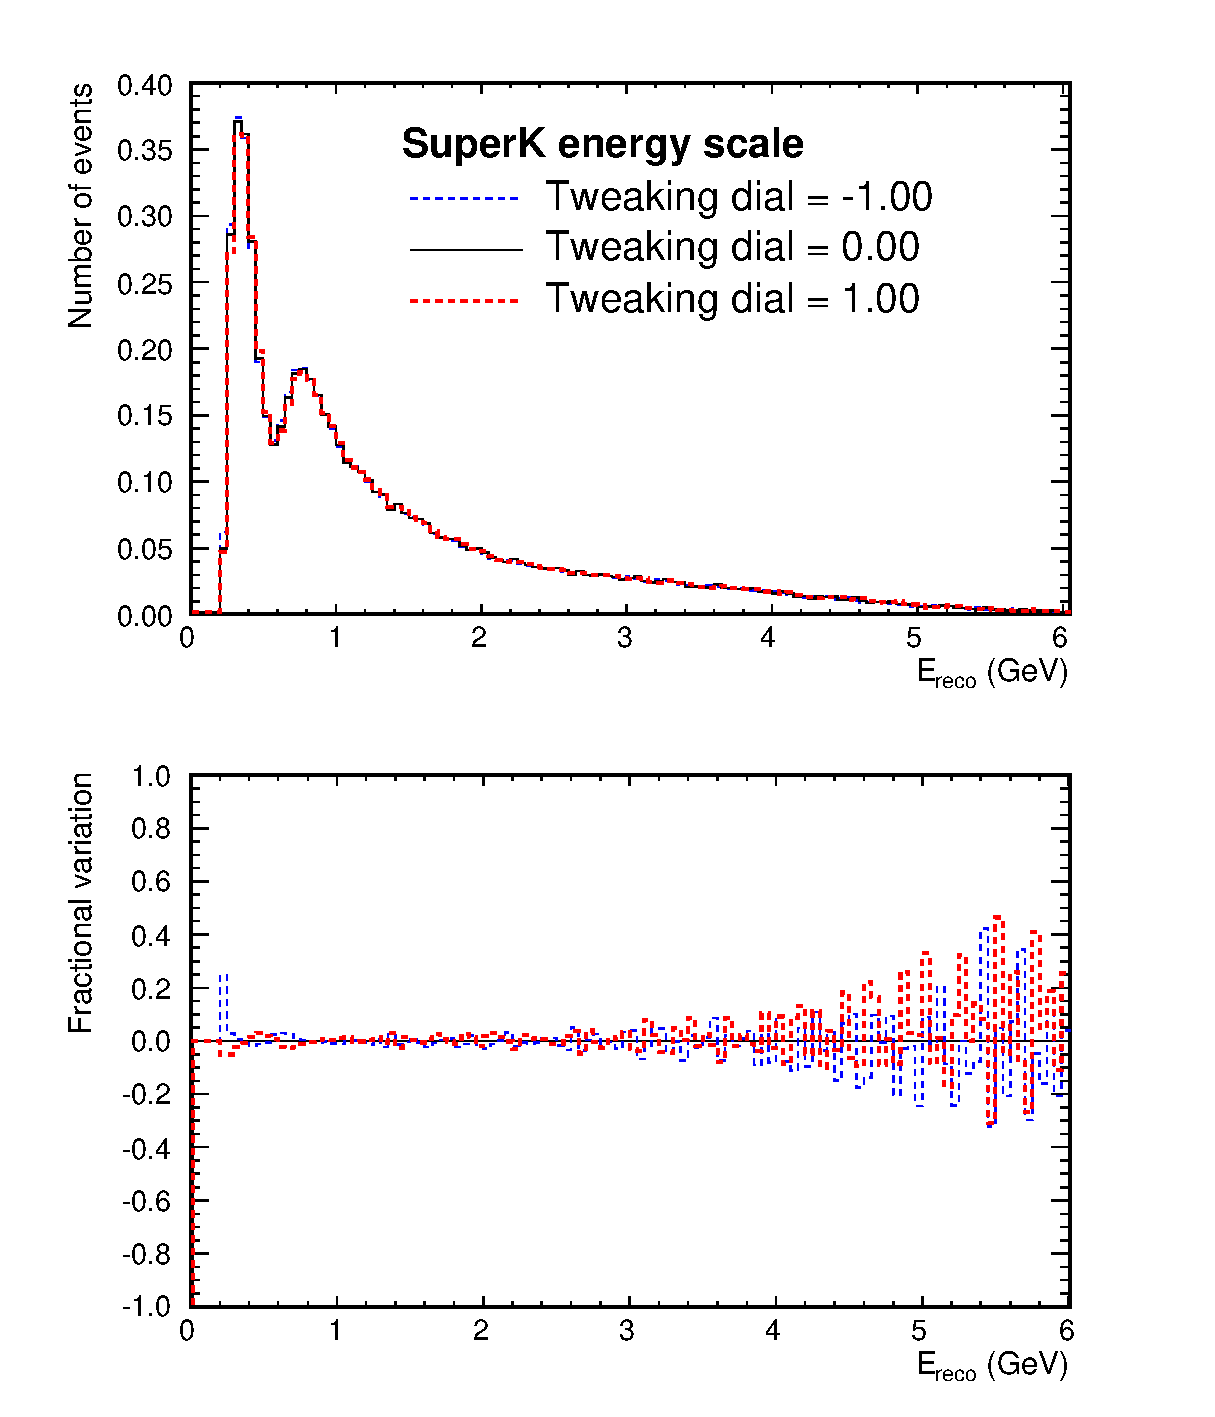
\includegraphics[width=19pc,height=21pc]{./images/predicted_spectrum/systematic_variations/genie_sk_spectrum_twk_skescale_2p4Em3_1p0.eps}
\caption{
  Effect of SuperK energy scale variation to the GENIE
  reconstructed-energy spectrum of 1-ring muon-like events (after extrapolation).
  All spectra have oscillations with $sin^{2}2\theta_{23}$ = 1.0 and $\Delta m^{2}_{23}$ = 2.4$\times10^{-3}$ $eV^{2}/c^{4}$ applied.  
}
\label{fig:genie_sk_spectrum_twk_skescale_2p4Em3_1p0}
\end{minipage}
\hspace{0.06\linewidth}
\begin{minipage}[t]{0.47\linewidth}
\centering
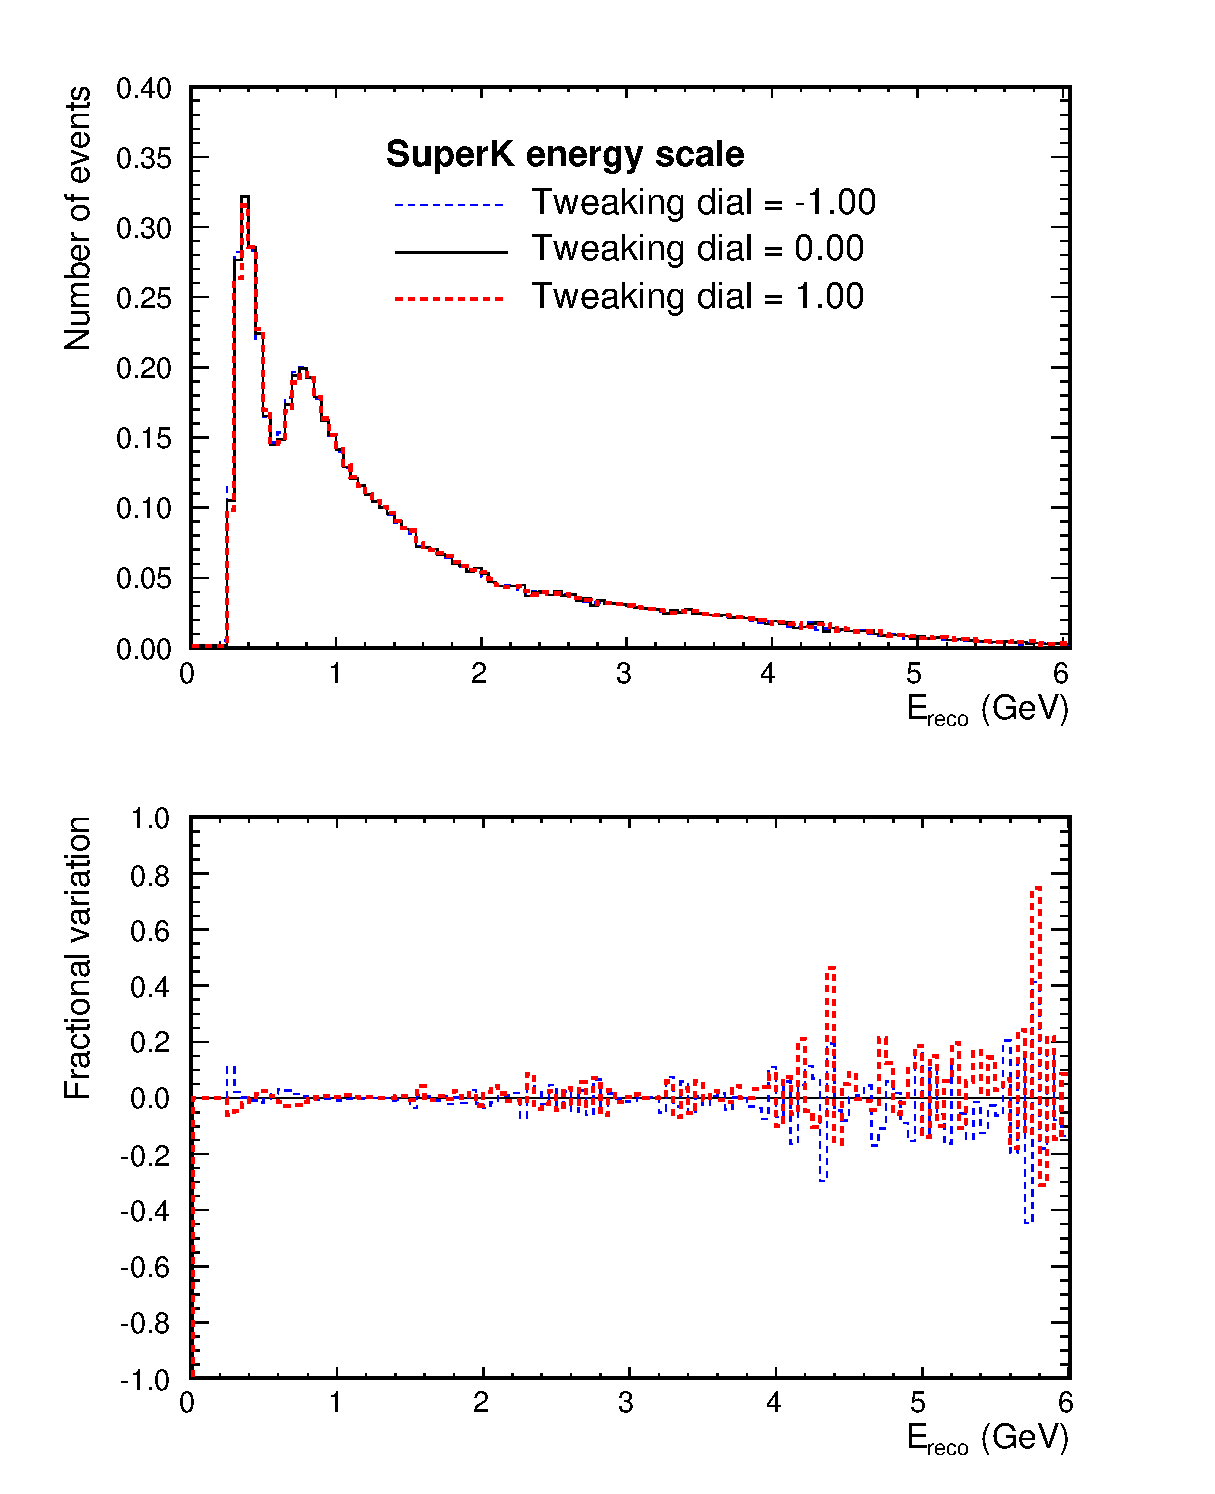
\includegraphics[width=19pc,height=21pc]{images/predicted_spectrum/systematic_variations/neut_sk_spectrum_twk_skescale_2p4Em3_1p0.eps}
\caption{
  Effect of SuperK energy scale variation to the NEUT
  reconstructed-energy spectrum of 1-ring muon-like events (after extrapolation).
  All spectra have oscillations with $sin^{2}2\theta_{23}$ = 1.0 and $\Delta m^{2}_{23}$ = 2.4$\times10^{-3}$ $eV^{2}/c^{4}$ applied.  
}
\label{fig:neut_sk_spectrum_twk_skescale_2p4Em3_1p0}
\end{minipage}
\end{figure}

%
% nd280 efficiency
%

\begin{figure}[ht]
\begin{minipage}[t]{0.47\linewidth}
\centering
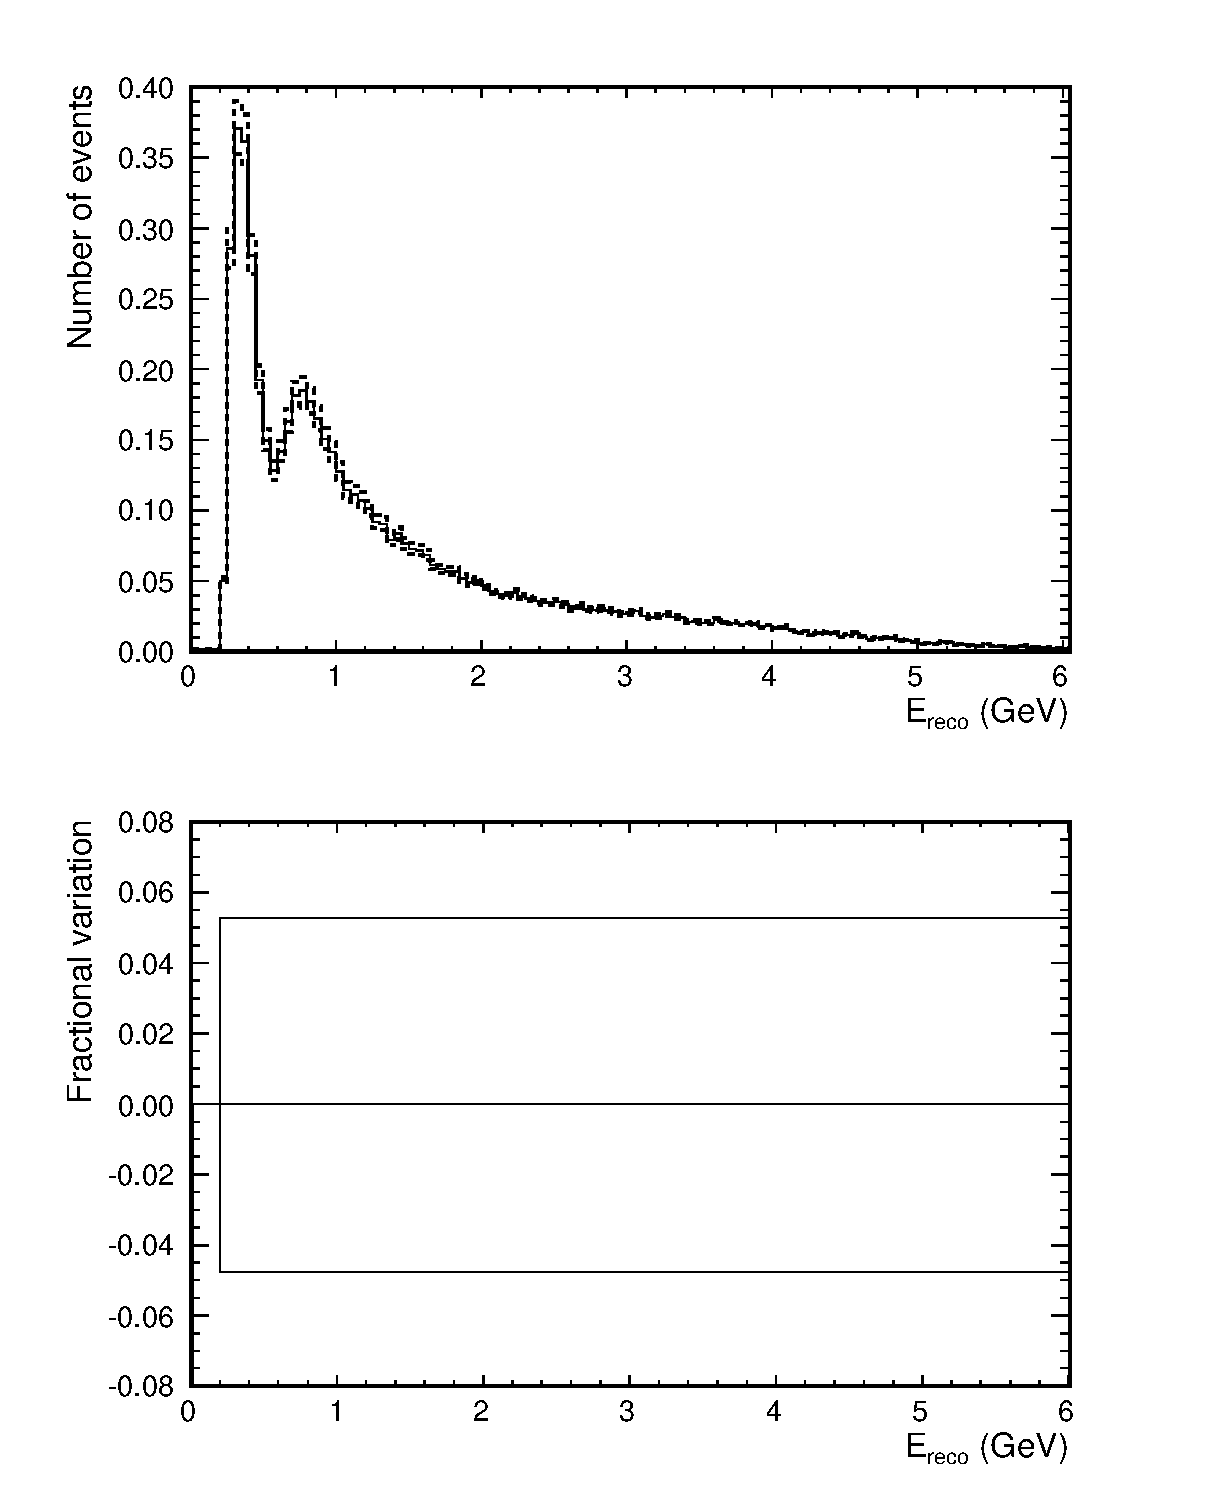
\includegraphics[width=19pc,height=21pc]{./images/predicted_spectrum/systematic_variations/genie_sk_spectrum_twk_nd280eff_2p4Em3_1p0.eps}
\caption{
  Effect of ND280 efficiency variation to the GENIE
  reconstructed-energy spectrum of 1-ring muon-like events (after extrapolation).
  All spectra have oscillations with $sin^{2}2\theta_{23}$ = 1.0 and $\Delta m^{2}_{23}$ = 2.4$\times10^{-3}$ $eV^{2}/c^{4}$ applied.  
}
\label{fig:genie_sk_spectrum_twk_nd280eff_2p4Em3_1p0}
\end{minipage}
\hspace{0.06\linewidth}
\begin{minipage}[t]{0.47\linewidth}
\centering
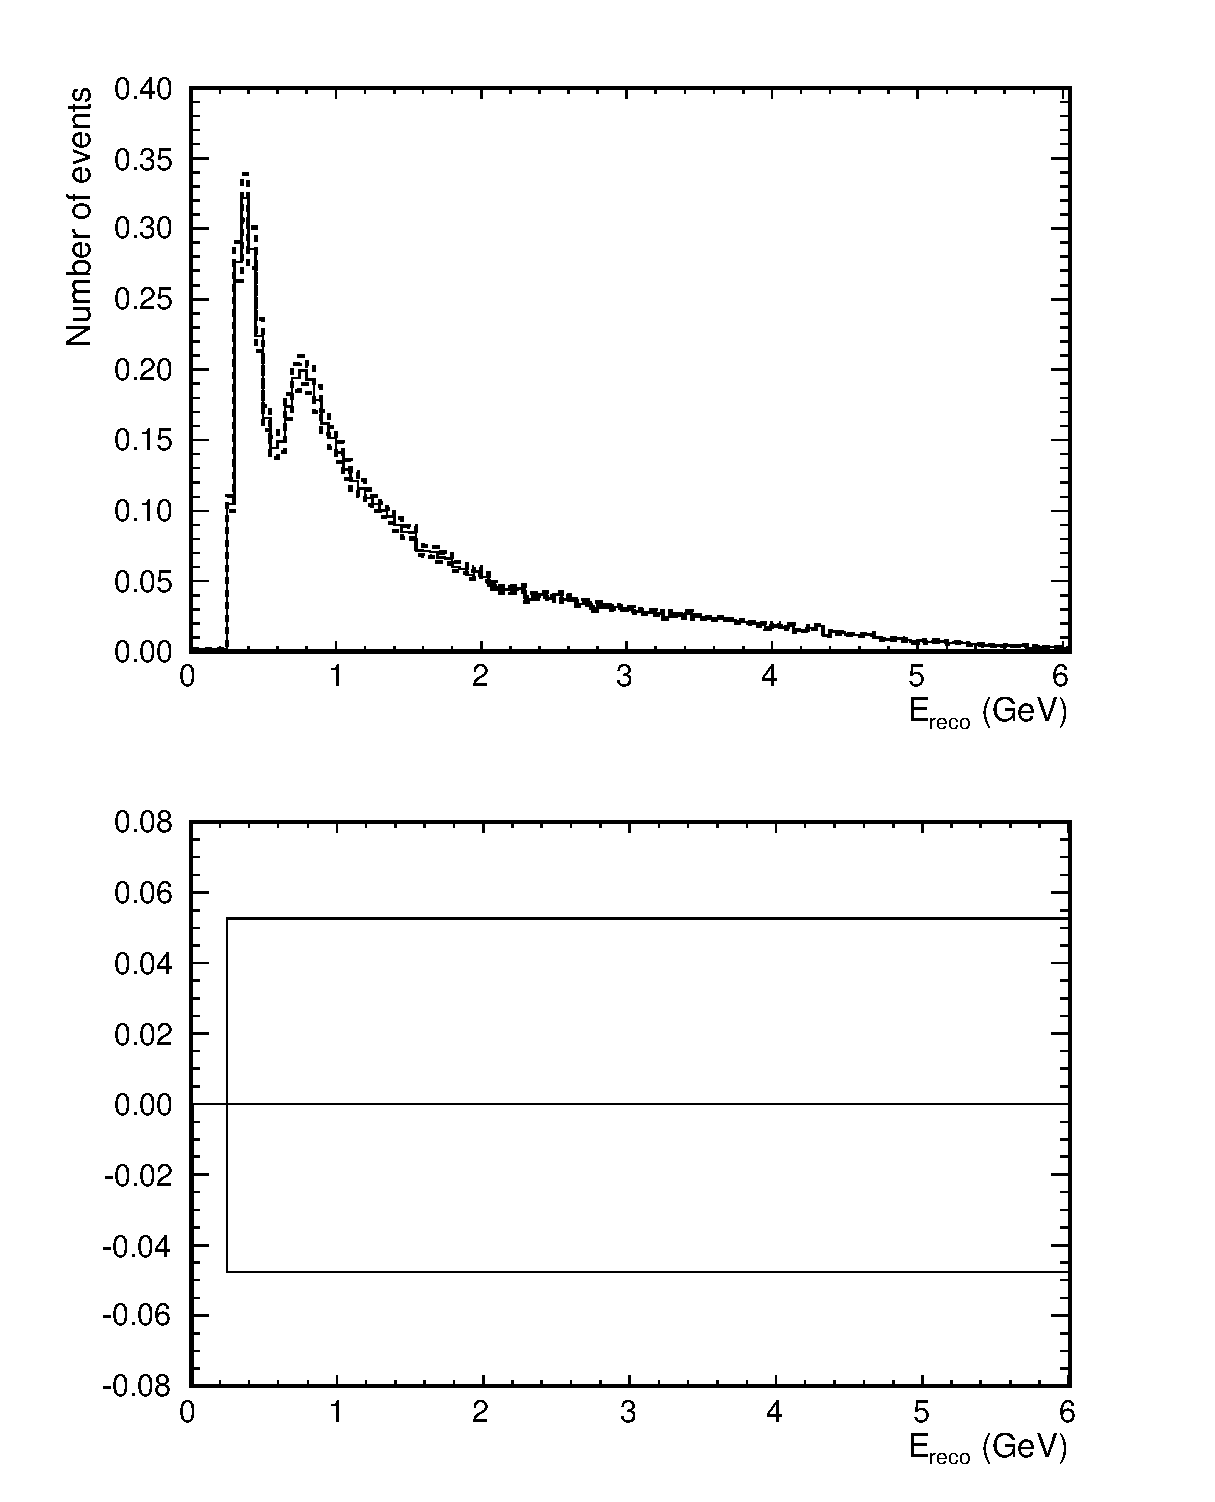
\includegraphics[width=19pc,height=21pc]{images/predicted_spectrum/systematic_variations/neut_sk_spectrum_twk_nd280eff_2p4Em3_1p0.eps}
\caption{
  Effect of ND280 efficiency variation to the NEUT
  reconstructed-energy spectrum of 1-ring muon-like events (after extrapolation).
  All spectra have oscillations with $sin^{2}2\theta_{23}$ = 1.0 and $\Delta m^{2}_{23}$ = 2.4$\times10^{-3}$ $eV^{2}/c^{4}$ applied.  
}
\label{fig:neut_sk_spectrum_twk_nd280eff_2p4Em3_1p0}
\end{minipage}
\end{figure}


%
% Beam norm
%

\begin{figure}[ht]
\begin{minipage}[t]{0.47\linewidth}
\centering
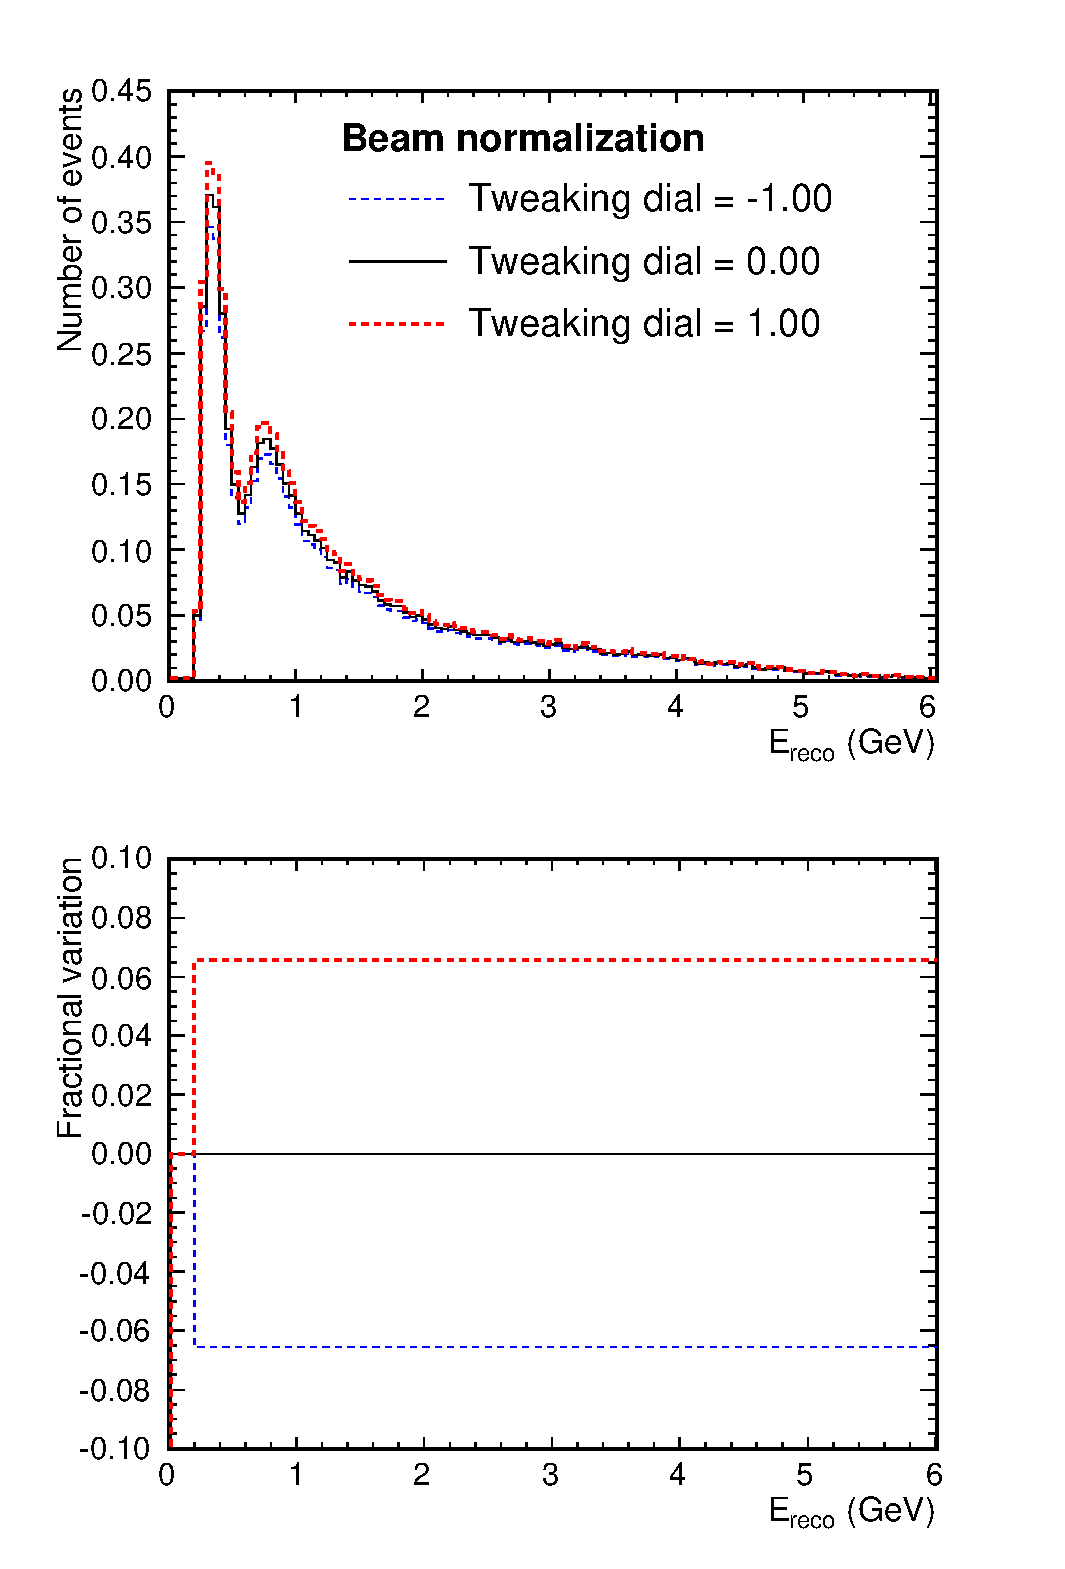
\includegraphics[width=17pc,height=17pc]{./images/predicted_spectrum/systematic_variations/genie_sk_spectrum_twk_bnorm_2p4Em3_1p0.eps}
\caption{
  Effect of beam normalization variation to the GENIE
  reconstructed-energy spectrum of 1-ring muon-like events (after extrapolation).
  All spectra have oscillations with $sin^{2}2\theta_{23}$ = 1.0 and $\Delta m^{2}_{23}$ = 2.4$\times10^{-3}$ $eV^{2}/c^{4}$ applied.  
}
\label{fig:genie_sk_spectrum_twk_bnorm_2p4Em3_1p0}
\end{minipage}
\hspace{0.06\linewidth}
\begin{minipage}[t]{0.47\linewidth}
\centering
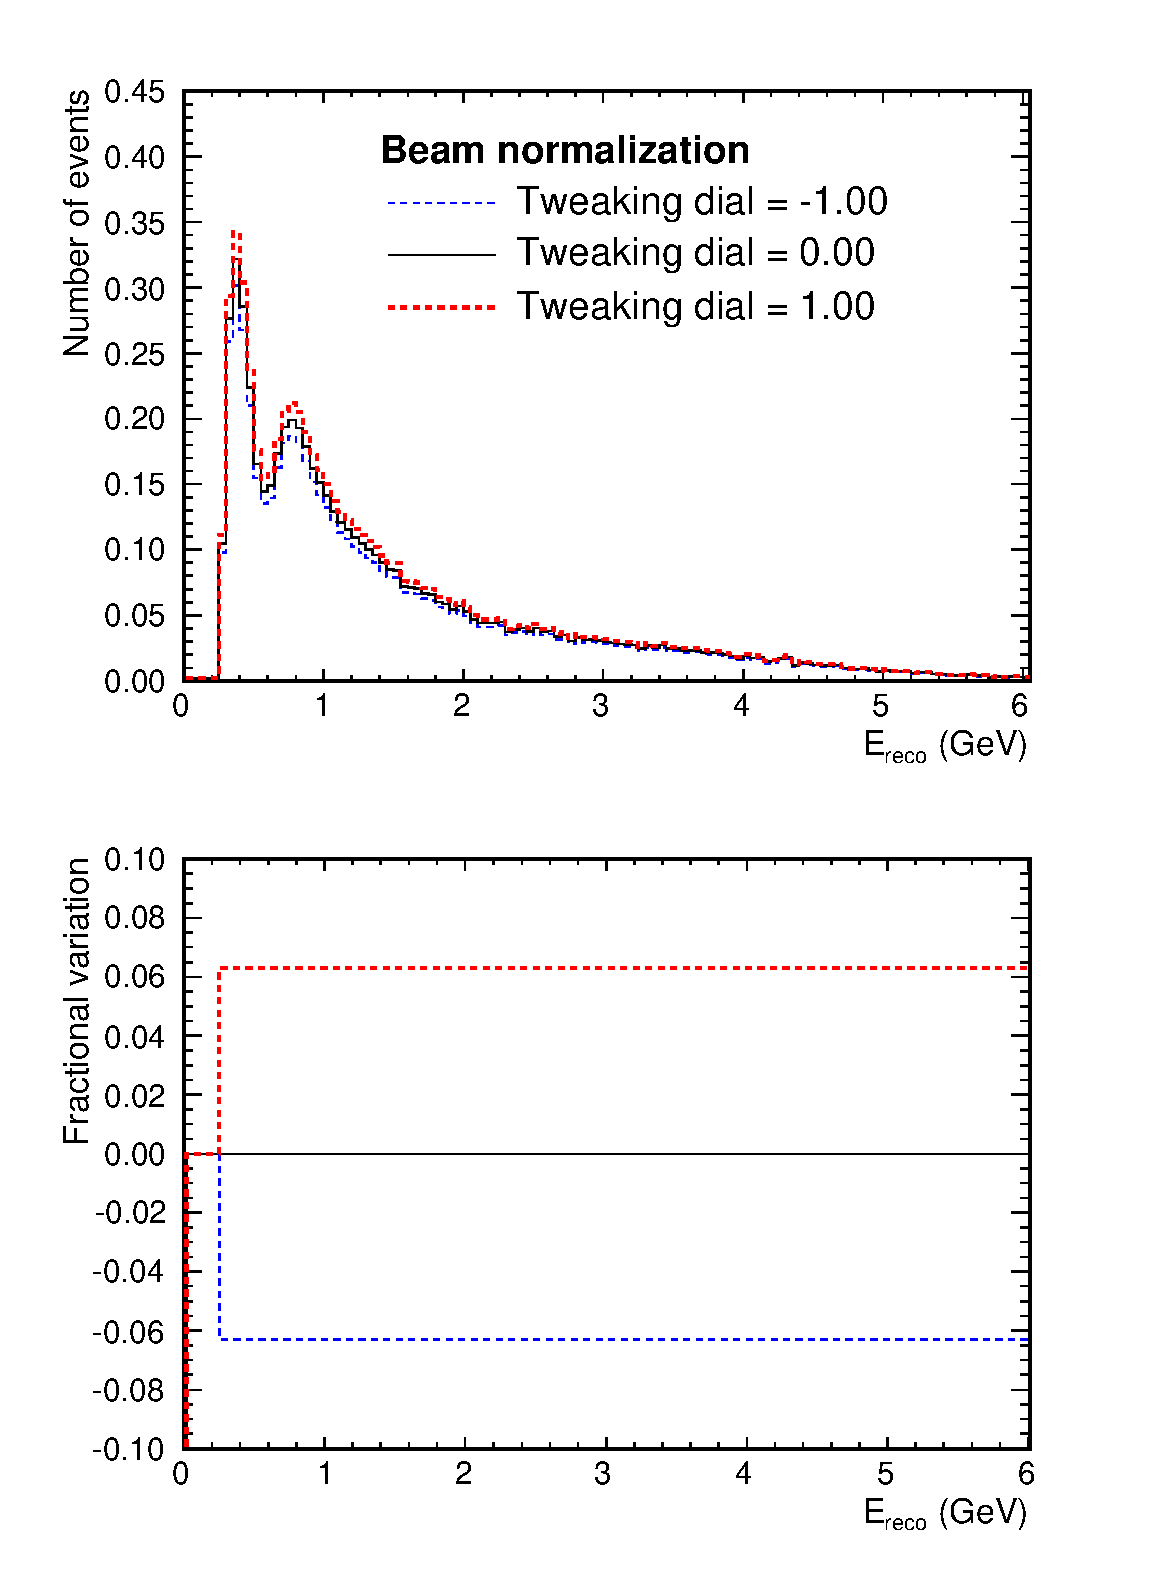
\includegraphics[width=17pc,height=17pc]{images/predicted_spectrum/systematic_variations/neut_sk_spectrum_twk_bnorm_2p4Em3_1p0.eps}
\caption{
  Effect of beam normalization variation to the NEUT
  reconstructed-energy spectrum of 1-ring muon-like events (after extrapolation).
  All spectra have oscillations with $sin^{2}2\theta_{23}$ = 1.0 and $\Delta m^{2}_{23}$ = 2.4$\times10^{-3}$ $eV^{2}/c^{4}$ applied.  
}
\label{fig:neut_sk_spectrum_twk_bnorm_2p4Em3_1p0}
\end{minipage}
\end{figure}

%
% Beam shape
%

\begin{figure}[ht]
\begin{minipage}[t]{0.47\linewidth}
\centering
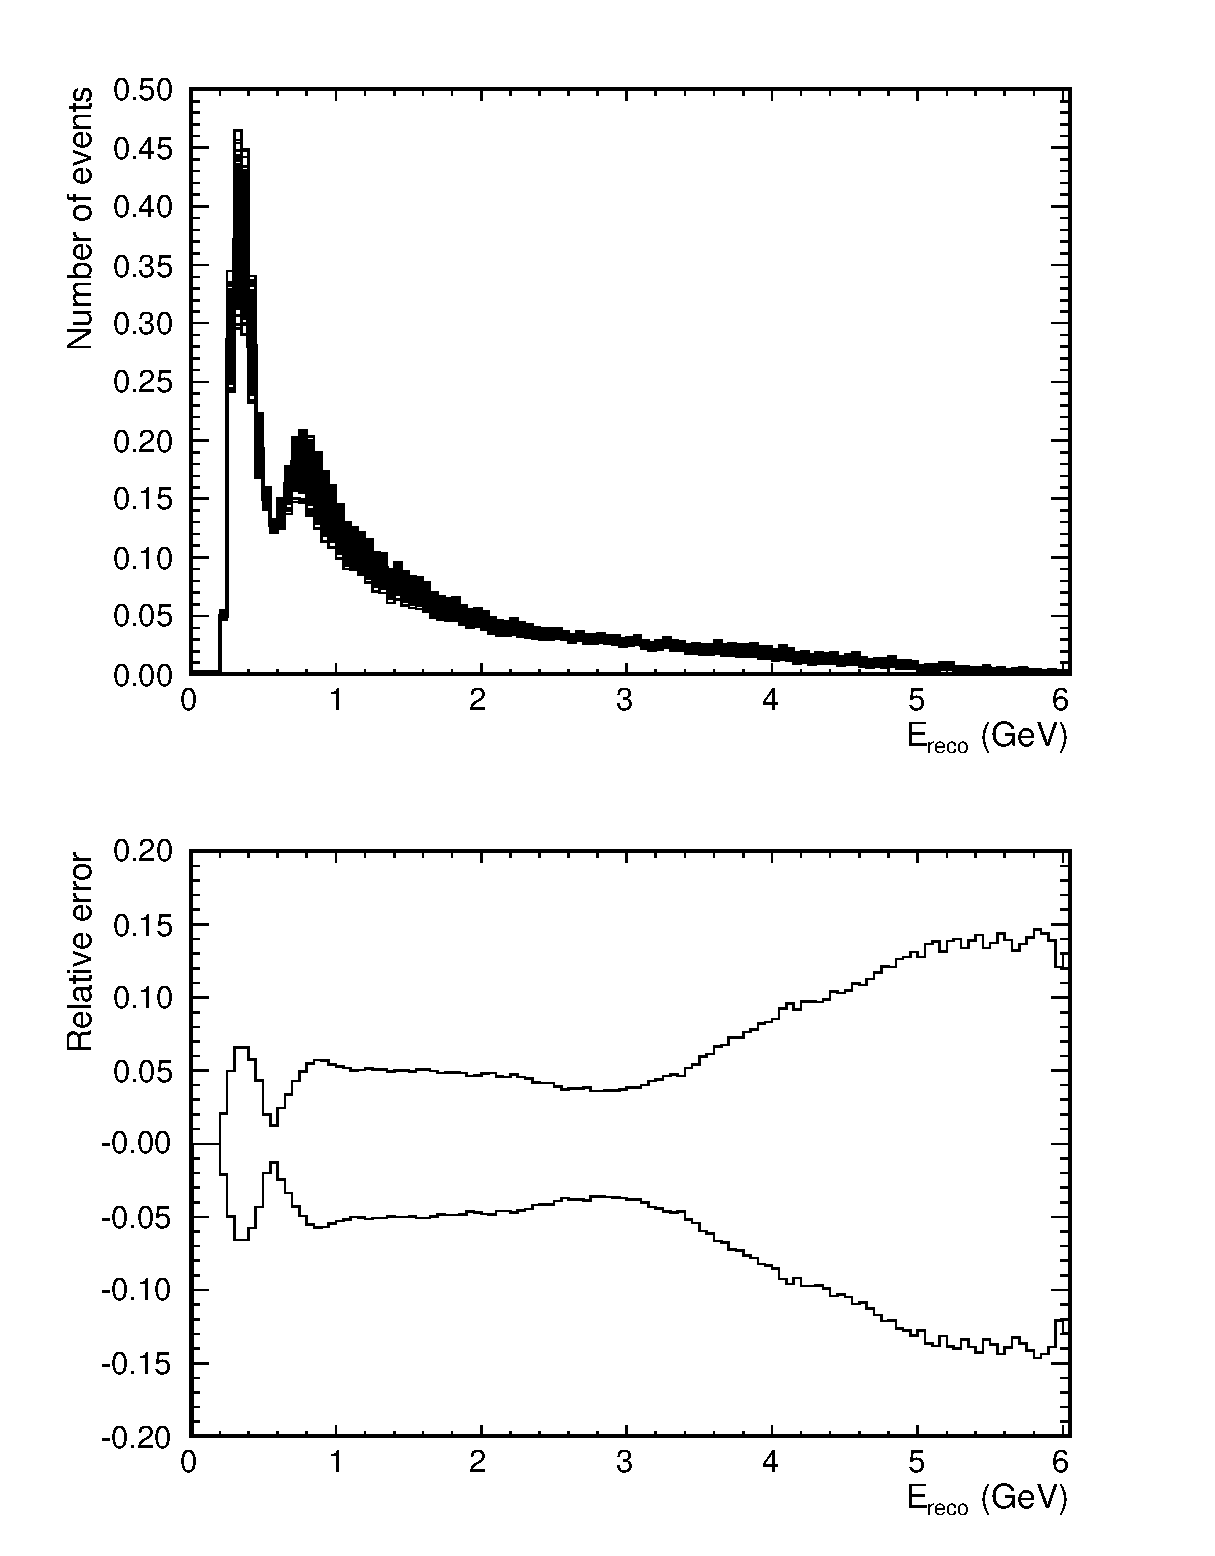
\includegraphics[width=19pc,height=19pc]{./images/predicted_spectrum/systematic_variations/genie_sk_spectrum_twk_bshape_2p4Em3_1p0.eps}
\caption{
  Effect of beam shape systematic variation to the GENIE
  reconstructed-energy spectrum of 1-ring muon-like events (after extrapolation).
  The top plot shows 2000 reconstructed-energy spectra corresponding 
  to 2000 fluxes generated using the Cholesky method (see Sec. \ref{sec:cholesky}).
  All spectra have oscillations with $sin^{2}2\theta_{23}$ = 1.0 and $\Delta m^{2}_{23}$ = 2.4$\times10^{-3}$ $eV^{2}/c^{4}$ applied
  and they are normalized to the number of events predicted using the nominal flux.
  The relative error shown in the bottom plot is calculated from the standard deviation of the randomly generated spectra.
}
\label{fig:genie_sk_spectrum_twk_bshape_2p4Em3_1p0}
\end{minipage}
\hspace{0.06\linewidth}
\begin{minipage}[t]{0.47\linewidth}
\centering
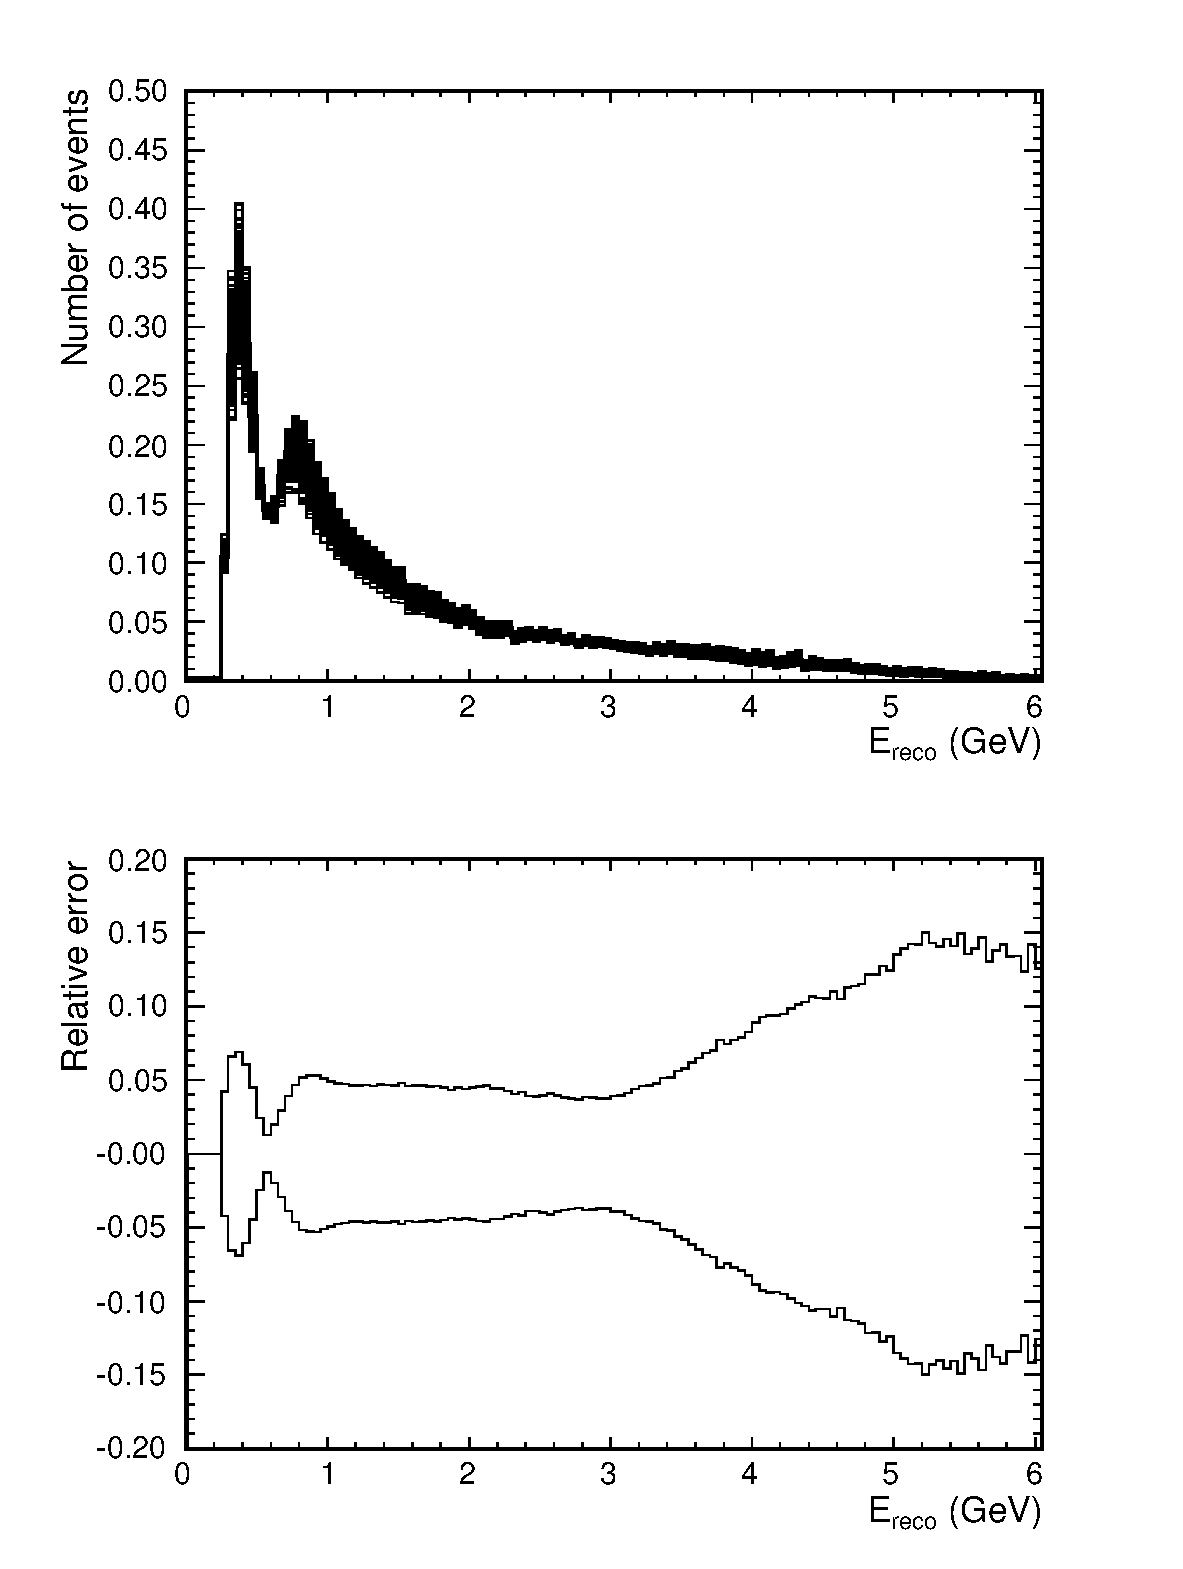
\includegraphics[width=19pc,height=19pc]{images/predicted_spectrum/systematic_variations/neut_sk_spectrum_twk_bshape_2p4Em3_1p0.eps}
\caption{
  Effect of beam shape variation to the NEUT
  reconstructed-energy spectrum of 1-ring muon-like events (after extrapolation).
  The plots were generated as described in Fig. \ref{fig:genie_sk_spectrum_twk_bshape_2p4Em3_1p0}.
}
\label{fig:neut_sk_spectrum_twk_bshape_2p4Em3_1p0}
\end{minipage}
\end{figure}


%
% CCQE
%

\begin{figure}[ht]
\begin{minipage}[t]{0.47\linewidth}
\centering
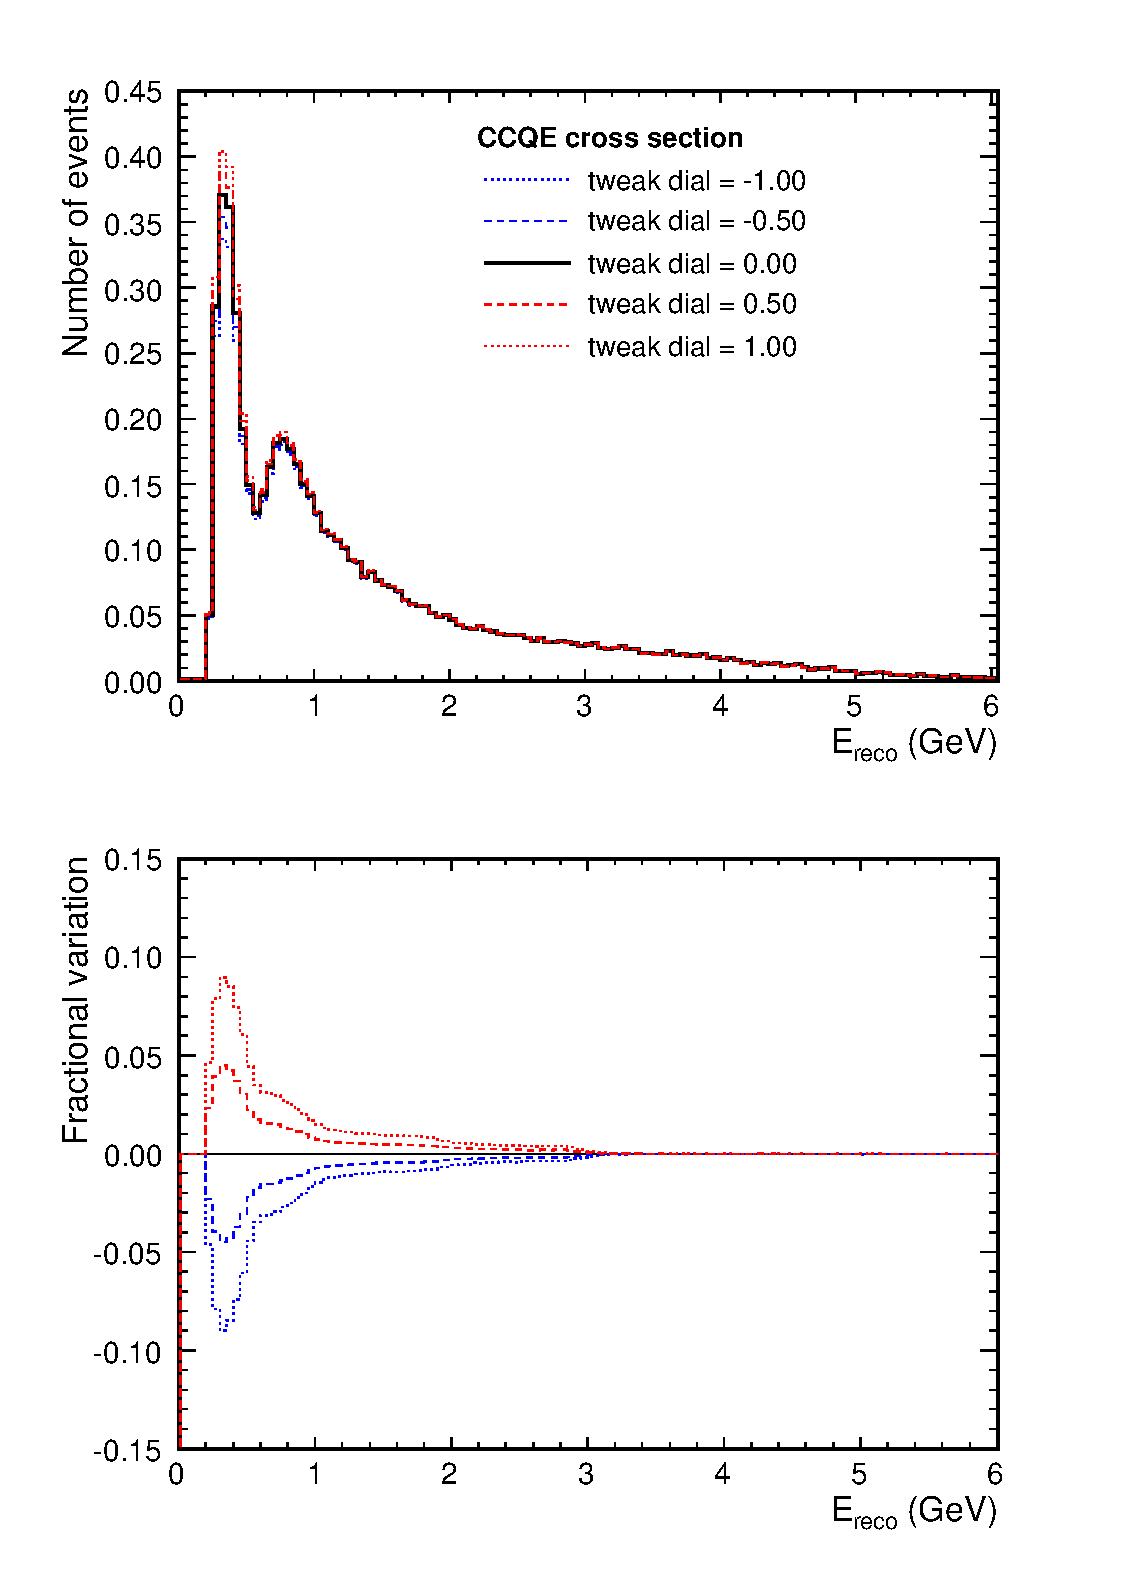
\includegraphics[width=19pc,height=21pc]{./images/predicted_spectrum/systematic_variations/genie_sk_spectrum_twk_ccqe_2p4Em3_1p0.eps}
\caption{
  Effect of CCQE cross section variation to the GENIE
  reconstructed-energy spectrum of 1-ring muon-like events (after extrapolation).
  All spectra have oscillations with $sin^{2}2\theta_{23}$ = 1.0 and $\Delta m^{2}_{23}$ = 2.4$\times10^{-3}$ $eV^{2}/c^{4}$ applied.  
}
\label{fig:genie_sk_spectrum_twk_ccqe_2p4Em3_1p0}
\end{minipage}
\hspace{0.06\linewidth}
\begin{minipage}[t]{0.47\linewidth}
\centering
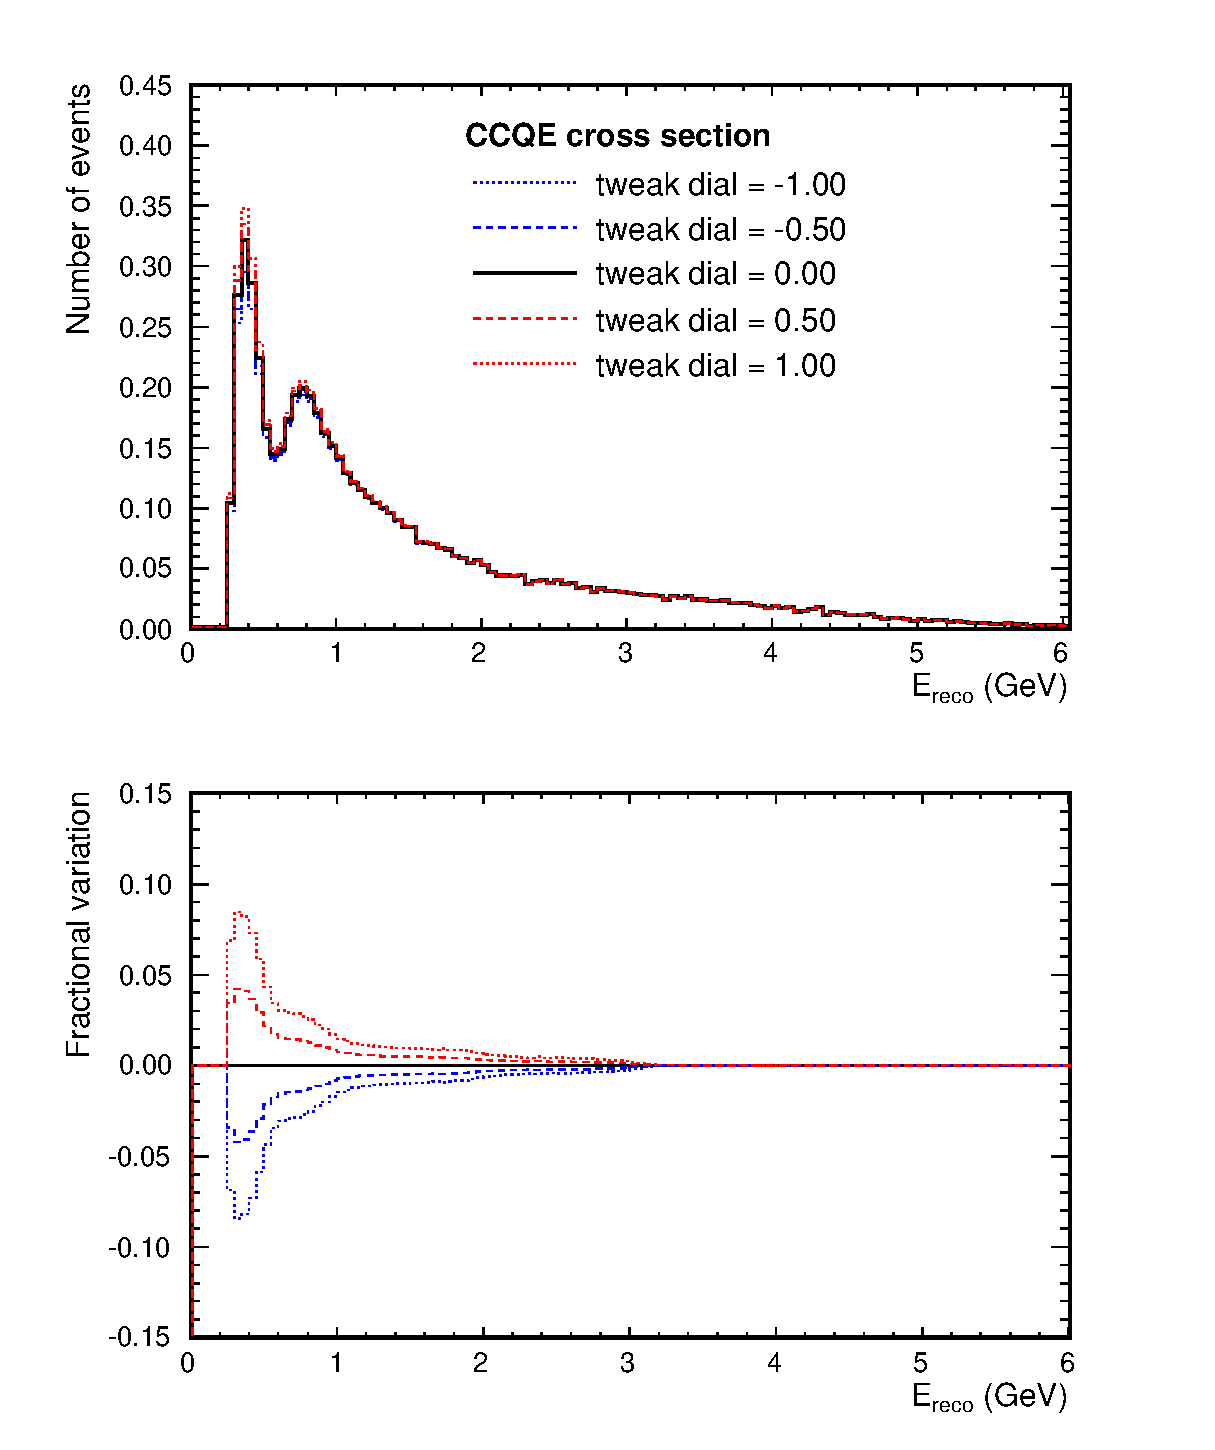
\includegraphics[width=19pc,height=21pc]{images/predicted_spectrum/systematic_variations/neut_sk_spectrum_twk_ccqe_2p4Em3_1p0.eps}
\caption{
  Effect of CCQE cross section variation to the NEUT
  reconstructed-energy spectrum of 1-ring muon-like events (after extrapolation).
  All spectra have oscillations with $sin^{2}2\theta_{23}$ = 1.0 and $\Delta m^{2}_{23}$ = 2.4$\times10^{-3}$ $eV^{2}/c^{4}$ applied.  
}
\label{fig:neut_sk_spectrum_twk_ccqe_2p4Em3_1p0}
\end{minipage}
\end{figure}

%
% CC1pi/CCQE
%

\begin{figure}[ht]
\begin{minipage}[t]{0.47\linewidth}
\centering
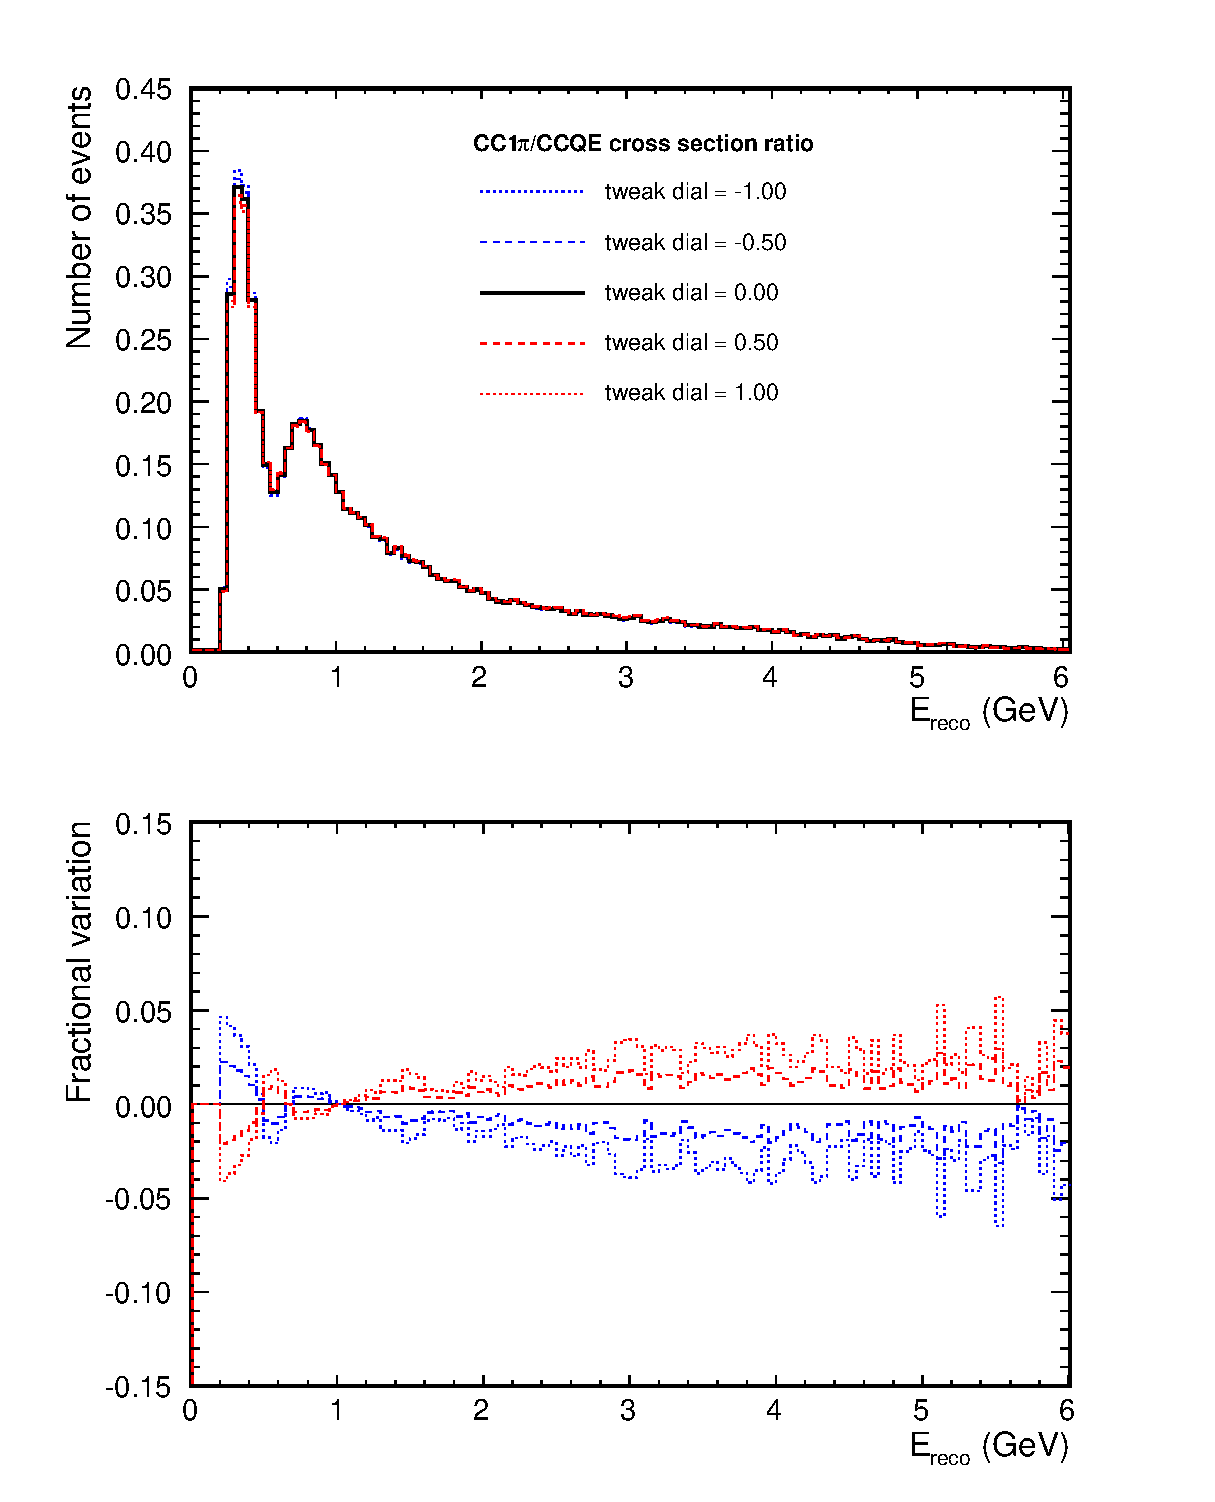
\includegraphics[width=19pc,height=21pc]{./images/predicted_spectrum/systematic_variations/genie_sk_spectrum_twk_cc1piccqe_2p4Em3_1p0.eps}
\caption{
  Effect of CC1$\pi$/CCQE cross section ratio variation to the GENIE
  reconstructed-energy spectrum of 1-ring muon-like events (after extrapolation).
  All spectra have oscillations with $sin^{2}2\theta_{23}$ = 1.0 and $\Delta m^{2}_{23}$ = 2.4$\times10^{-3}$ $eV^{2}/c^{4}$ applied.  
}
\label{fig:genie_sk_spectrum_twk_cc1piccqe_2p4Em3_1p0}
\end{minipage}
\hspace{0.06\linewidth}
\begin{minipage}[t]{0.47\linewidth}
\centering
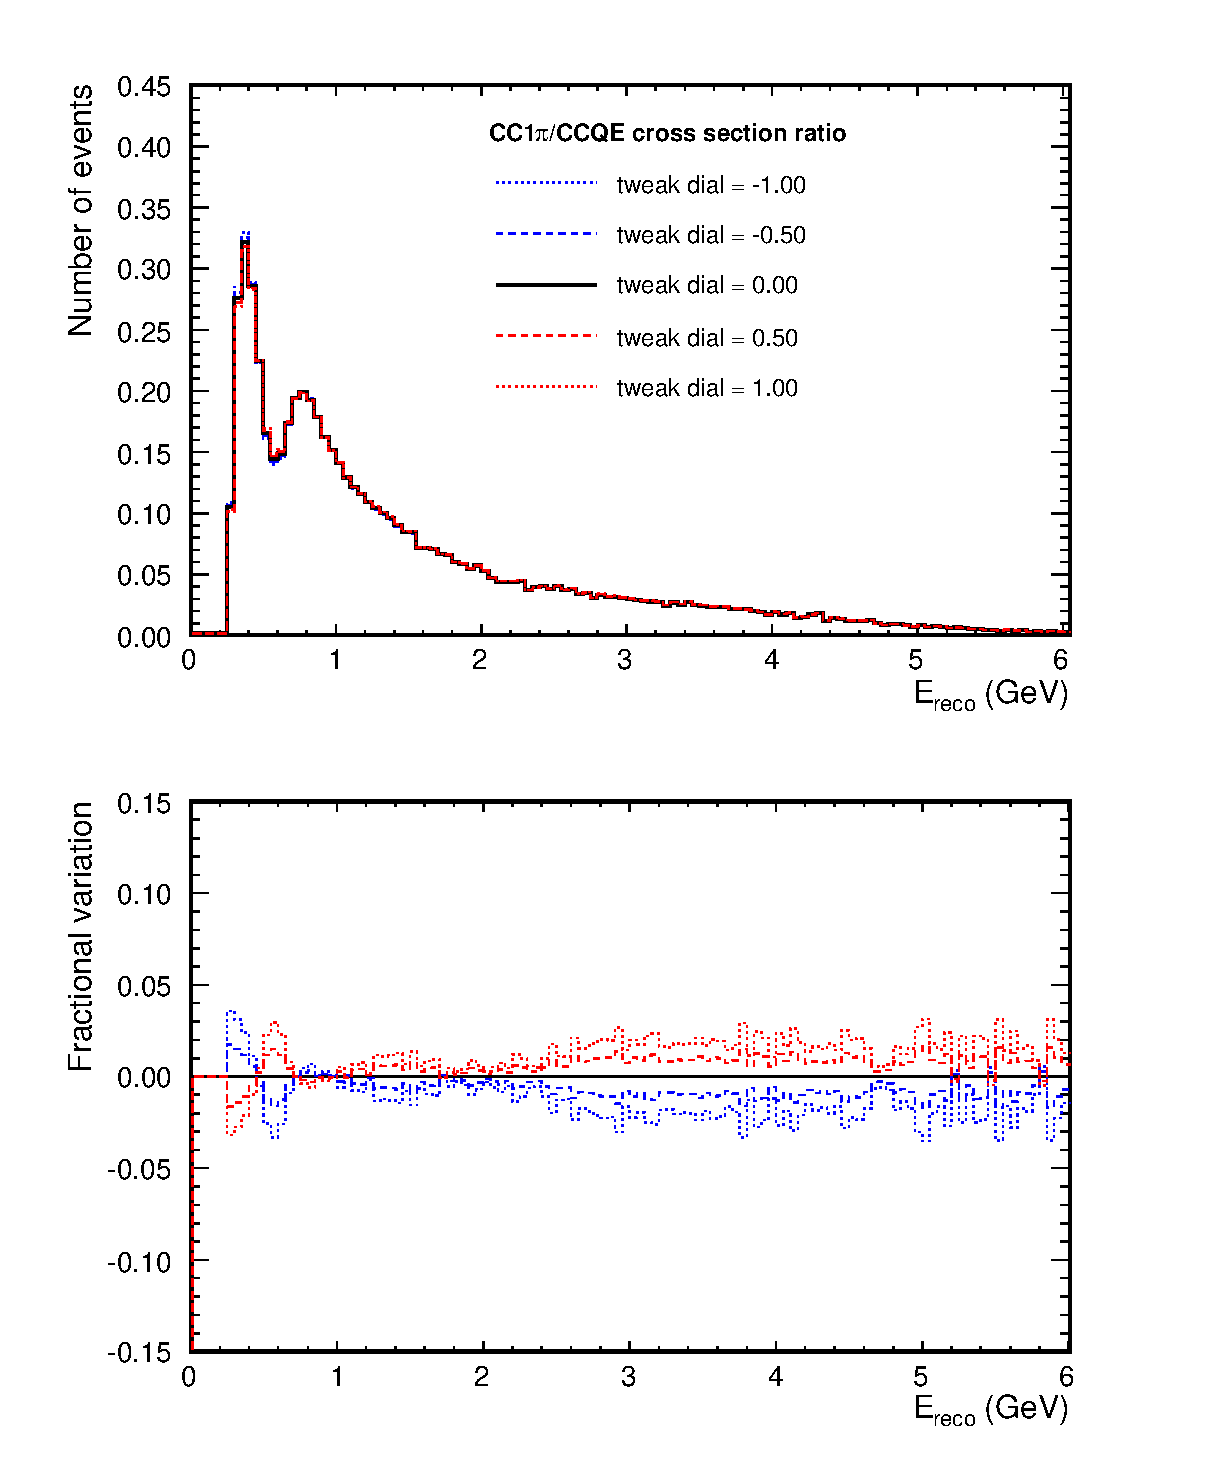
\includegraphics[width=19pc,height=21pc]{images/predicted_spectrum/systematic_variations/neut_sk_spectrum_twk_cc1piccqe_2p4Em3_1p0.eps}
\caption{
  Effect of CC1$\pi$/CCQE cross section ratio variation to the NEUT
  reconstructed-energy spectrum of 1-ring muon-like events (after extrapolation).
  All spectra have oscillations with $sin^{2}2\theta_{23}$ = 1.0 and $\Delta m^{2}_{23}$ = 2.4$\times10^{-3}$ $eV^{2}/c^{4}$ applied.  
}
\label{fig:neut_sk_spectrum_twk_cc1piccqe_2p4Em3_1p0}
\end{minipage}
\end{figure}


%
% CCoth/CCQE
%

\begin{figure}[ht]
\begin{minipage}[t]{0.47\linewidth}
\centering
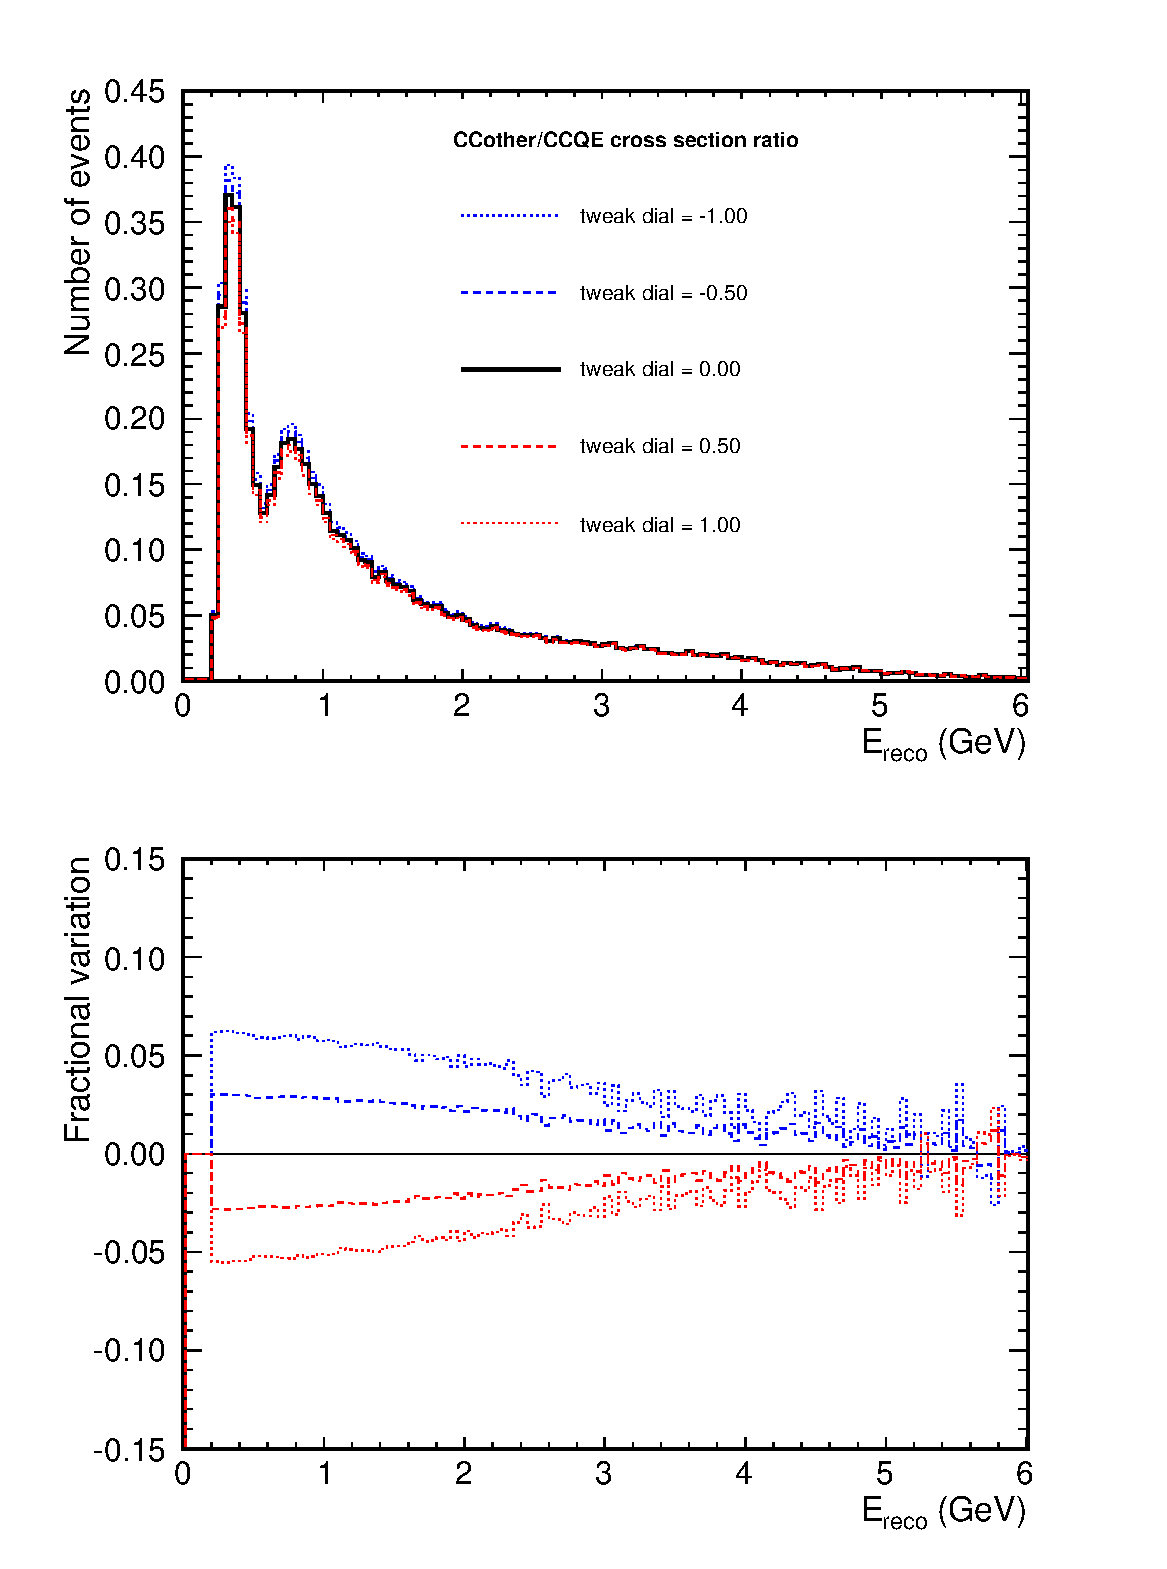
\includegraphics[width=19pc,height=21pc]{./images/predicted_spectrum/systematic_variations/genie_sk_spectrum_twk_ccothccqe_2p4Em3_1p0.eps}
\caption{
  Effect of CCother/CCQE cross section ratio variation to the GENIE
  reconstructed-energy spectrum of 1-ring muon-like events (after extrapolation).
  All spectra have oscillations with $sin^{2}2\theta_{23}$ = 1.0 and $\Delta m^{2}_{23}$ = 2.4$\times10^{-3}$ $eV^{2}/c^{4}$ applied.  
}
\label{fig:genie_sk_spectrum_twk_ccothccqe_2p4Em3_1p0}
\end{minipage}
\hspace{0.06\linewidth}
\begin{minipage}[t]{0.47\linewidth}
\centering
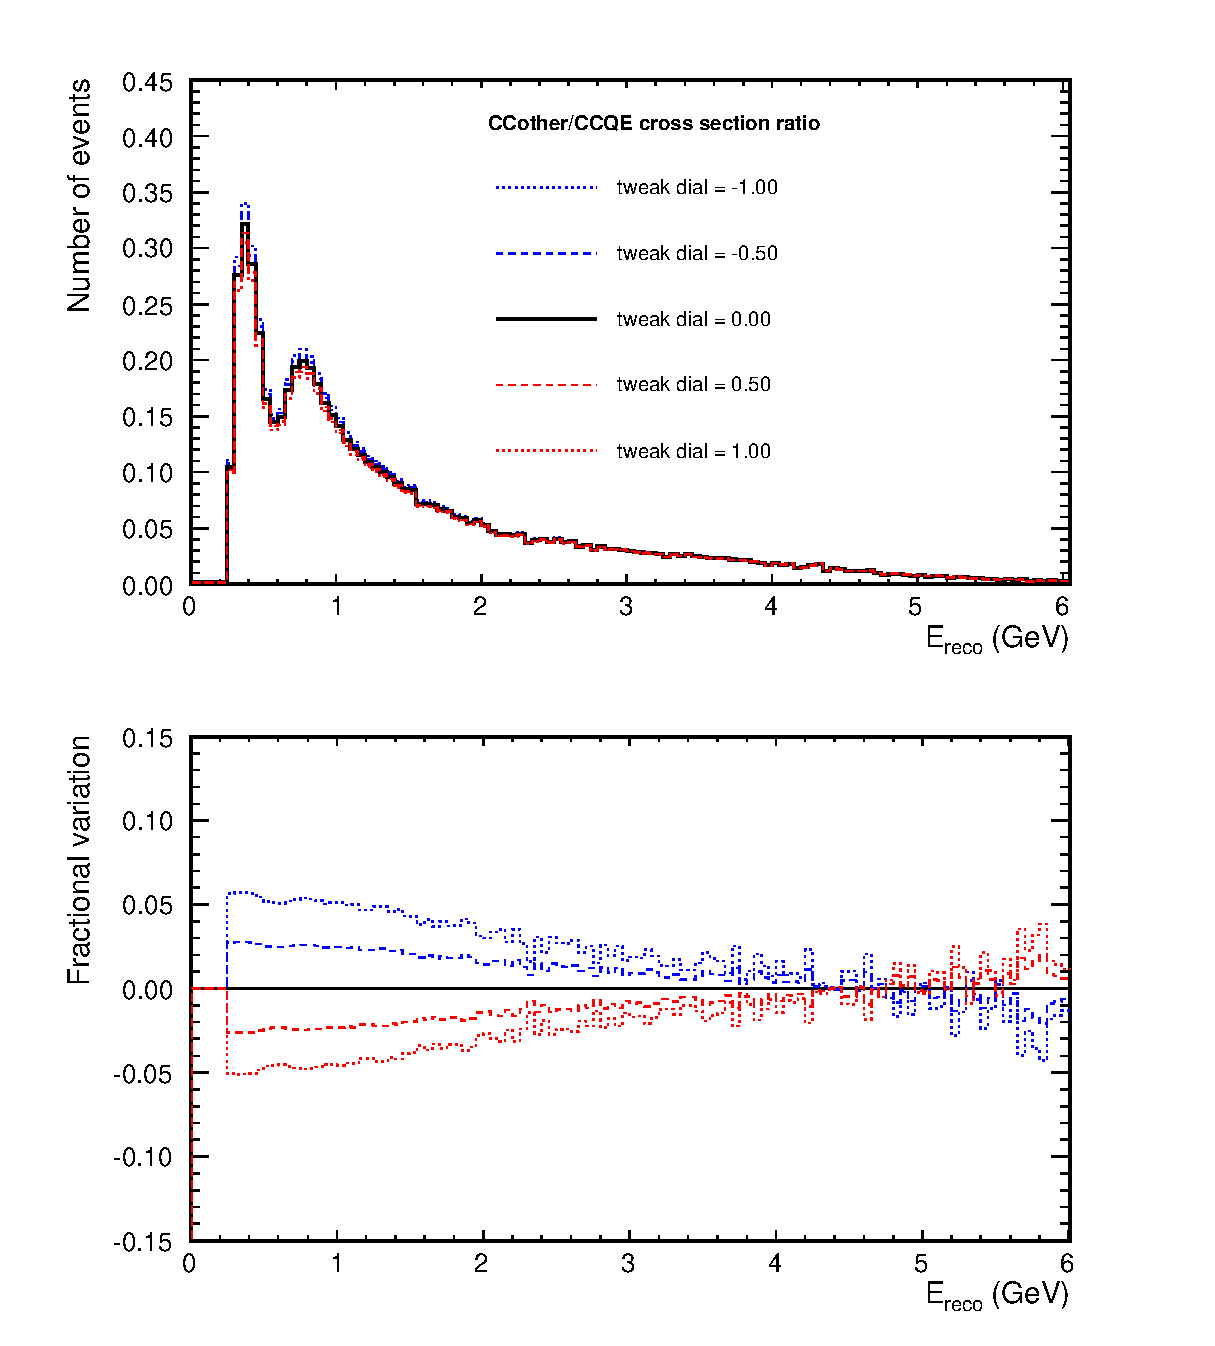
\includegraphics[width=19pc,height=21pc]{images/predicted_spectrum/systematic_variations/neut_sk_spectrum_twk_ccothccqe_2p4Em3_1p0.eps}
\caption{
  Effect of CCother/CCQE cross section ratio variation to the NEUT
  reconstructed-energy spectrum of 1-ring muon-like events (after extrapolation).
  All spectra have oscillations with $sin^{2}2\theta_{23}$ = 1.0 and $\Delta m^{2}_{23}$ = 2.4$\times10^{-3}$ $eV^{2}/c^{4}$ applied.  
}
\label{fig:neut_sk_spectrum_twk_ccothccqe_2p4Em3_1p0}
\end{minipage}
\end{figure}


%
% NC/CCQE
%

\begin{figure}[ht]
\begin{minipage}[t]{0.47\linewidth}
\centering
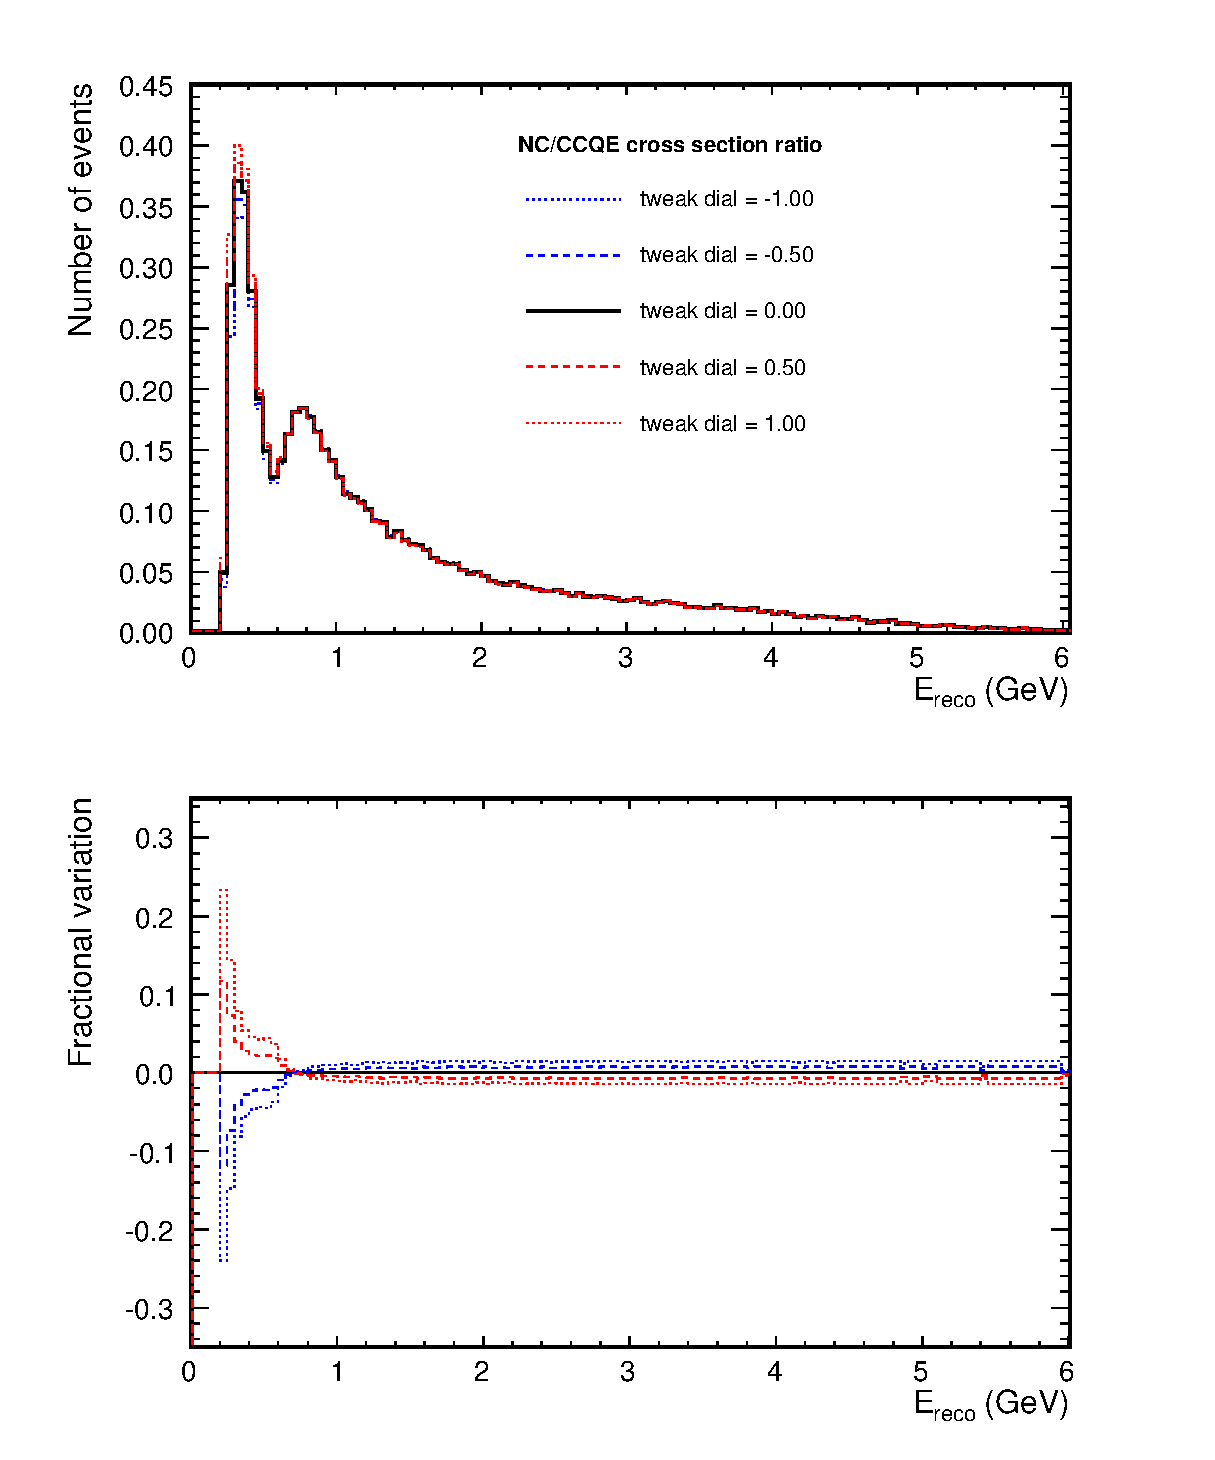
\includegraphics[width=19pc,height=21pc]{./images/predicted_spectrum/systematic_variations/genie_sk_spectrum_twk_ncccqe_2p4Em3_1p0.eps}
\caption{
  Effect of NC/CCQE cross section ratio variation to the GENIE
  reconstructed-energy spectrum of 1-ring muon-like events (after extrapolation).
  All spectra have oscillations with $sin^{2}2\theta_{23}$ = 1.0 and $\Delta m^{2}_{23}$ = 2.4$\times10^{-3}$ $eV^{2}/c^{4}$ applied.  
}
\label{fig:genie_sk_spectrum_twk_ncccqe_2p4Em3_1p0}
\end{minipage}
\hspace{0.06\linewidth}
\begin{minipage}[t]{0.47\linewidth}
\centering
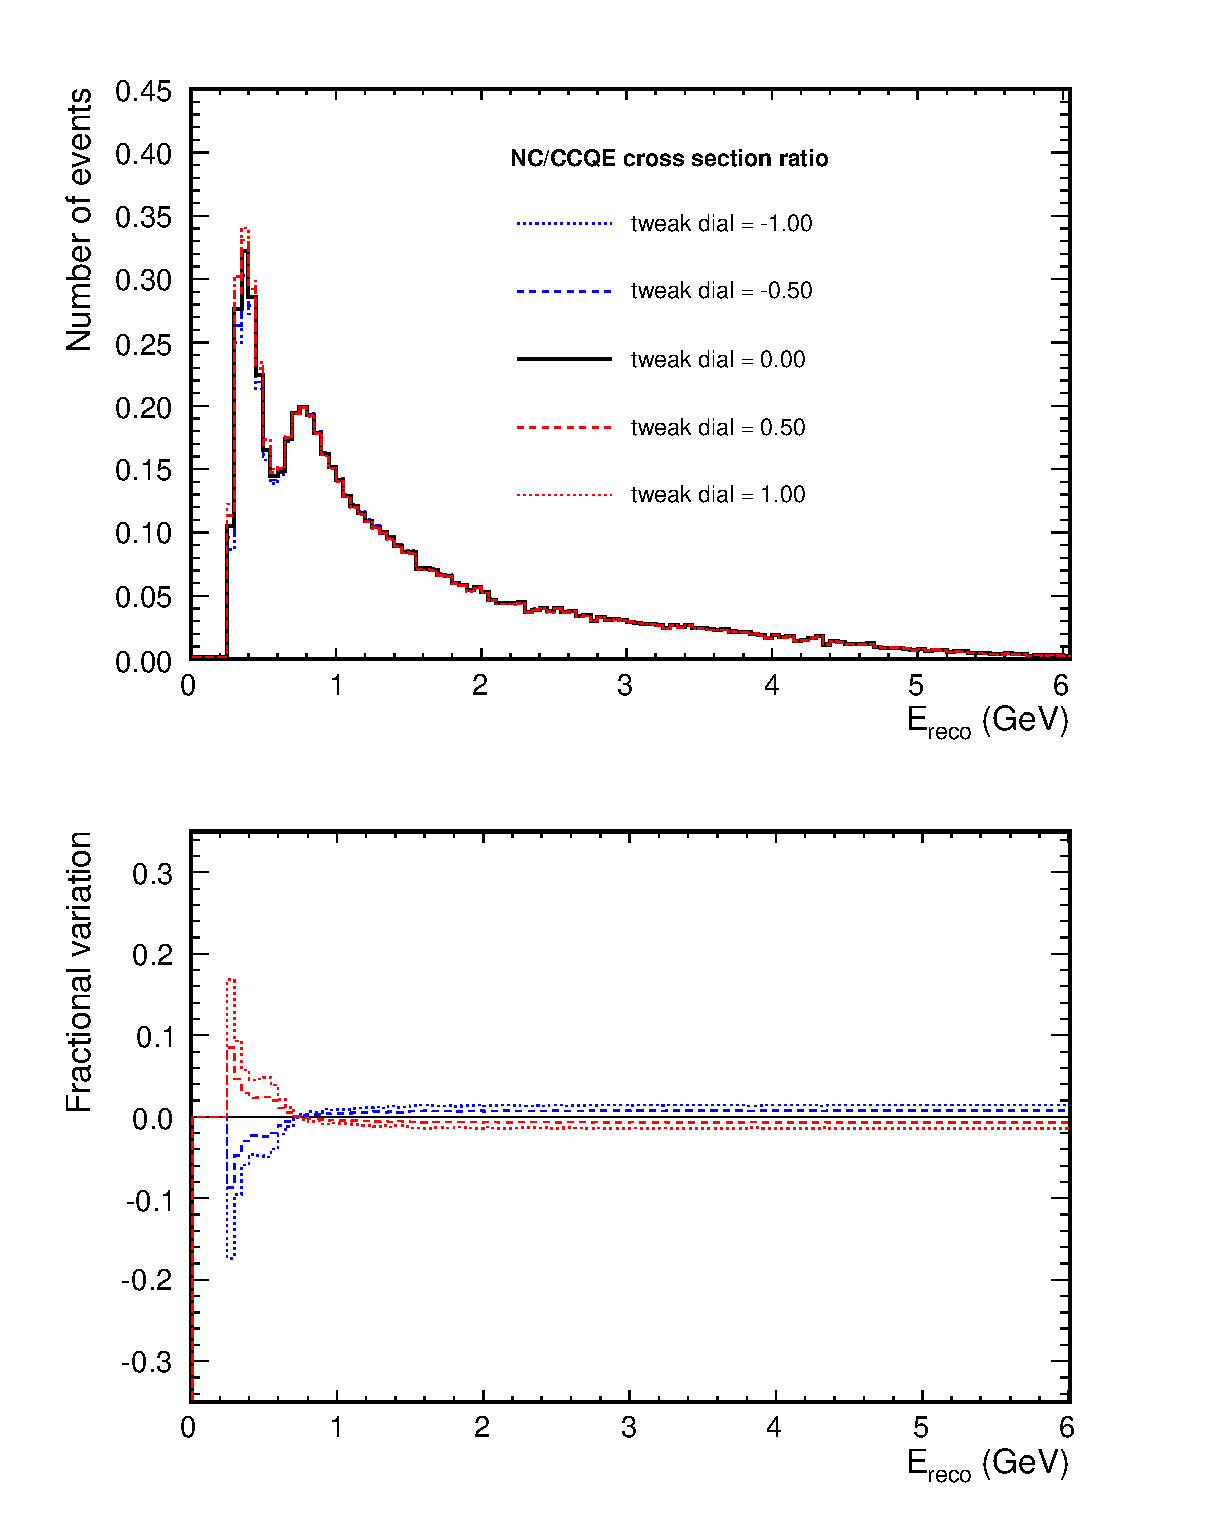
\includegraphics[width=19pc,height=21pc]{images/predicted_spectrum/systematic_variations/neut_sk_spectrum_twk_ncccqe_2p4Em3_1p0.eps}
\caption{
  Effect of NC/CCQE cross section ratio variation to the NEUT
  reconstructed-energy spectrum of 1-ring muon-like events (after extrapolation).
  All spectra have oscillations with $sin^{2}2\theta_{23}$ = 1.0 and $\Delta m^{2}_{23}$ = 2.4$\times10^{-3}$ $eV^{2}/c^{4}$ applied.  
}
\label{fig:neut_sk_spectrum_twk_ncccqe_2p4Em3_1p0}
\end{minipage}
\end{figure}


%
% NUCEFF
%

\begin{figure}[ht]
\begin{minipage}[t]{0.47\linewidth}
\centering
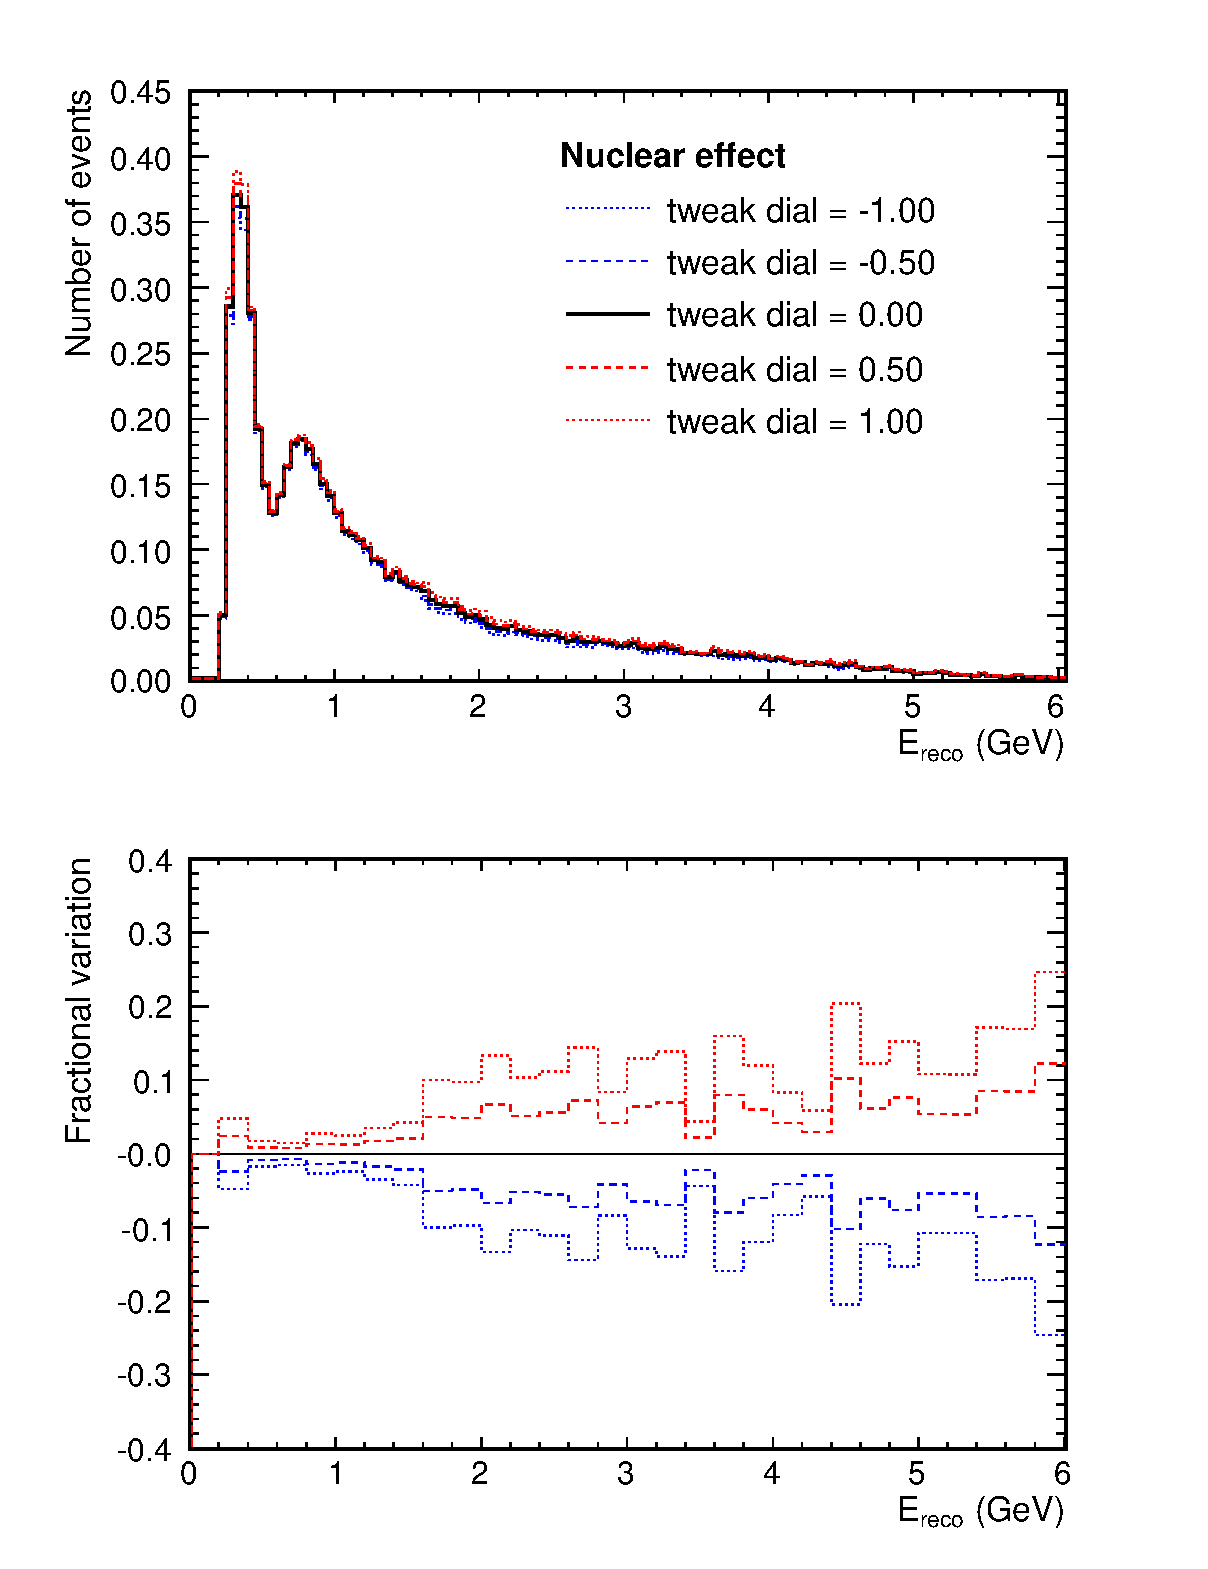
\includegraphics[width=19pc,height=21pc]{./images/predicted_spectrum/systematic_variations/genie_sk_spectrum_twk_nuceff_2p4Em3_1p0.eps}
\caption{
  Effect of FSI variation to the GENIE
  reconstructed-energy spectrum of 1-ring muon-like events (after extrapolation).
  All spectra have oscillations with $sin^{2}2\theta_{23}$ = 1.0 and $\Delta m^{2}_{23}$ = 2.4$\times10^{-3}$ $eV^{2}/c^{4}$ applied.  
}
\label{fig:genie_sk_spectrum_twk_nuceff_2p4Em3_1p0}
\end{minipage}
\hspace{0.06\linewidth}
\begin{minipage}[t]{0.47\linewidth}
\centering
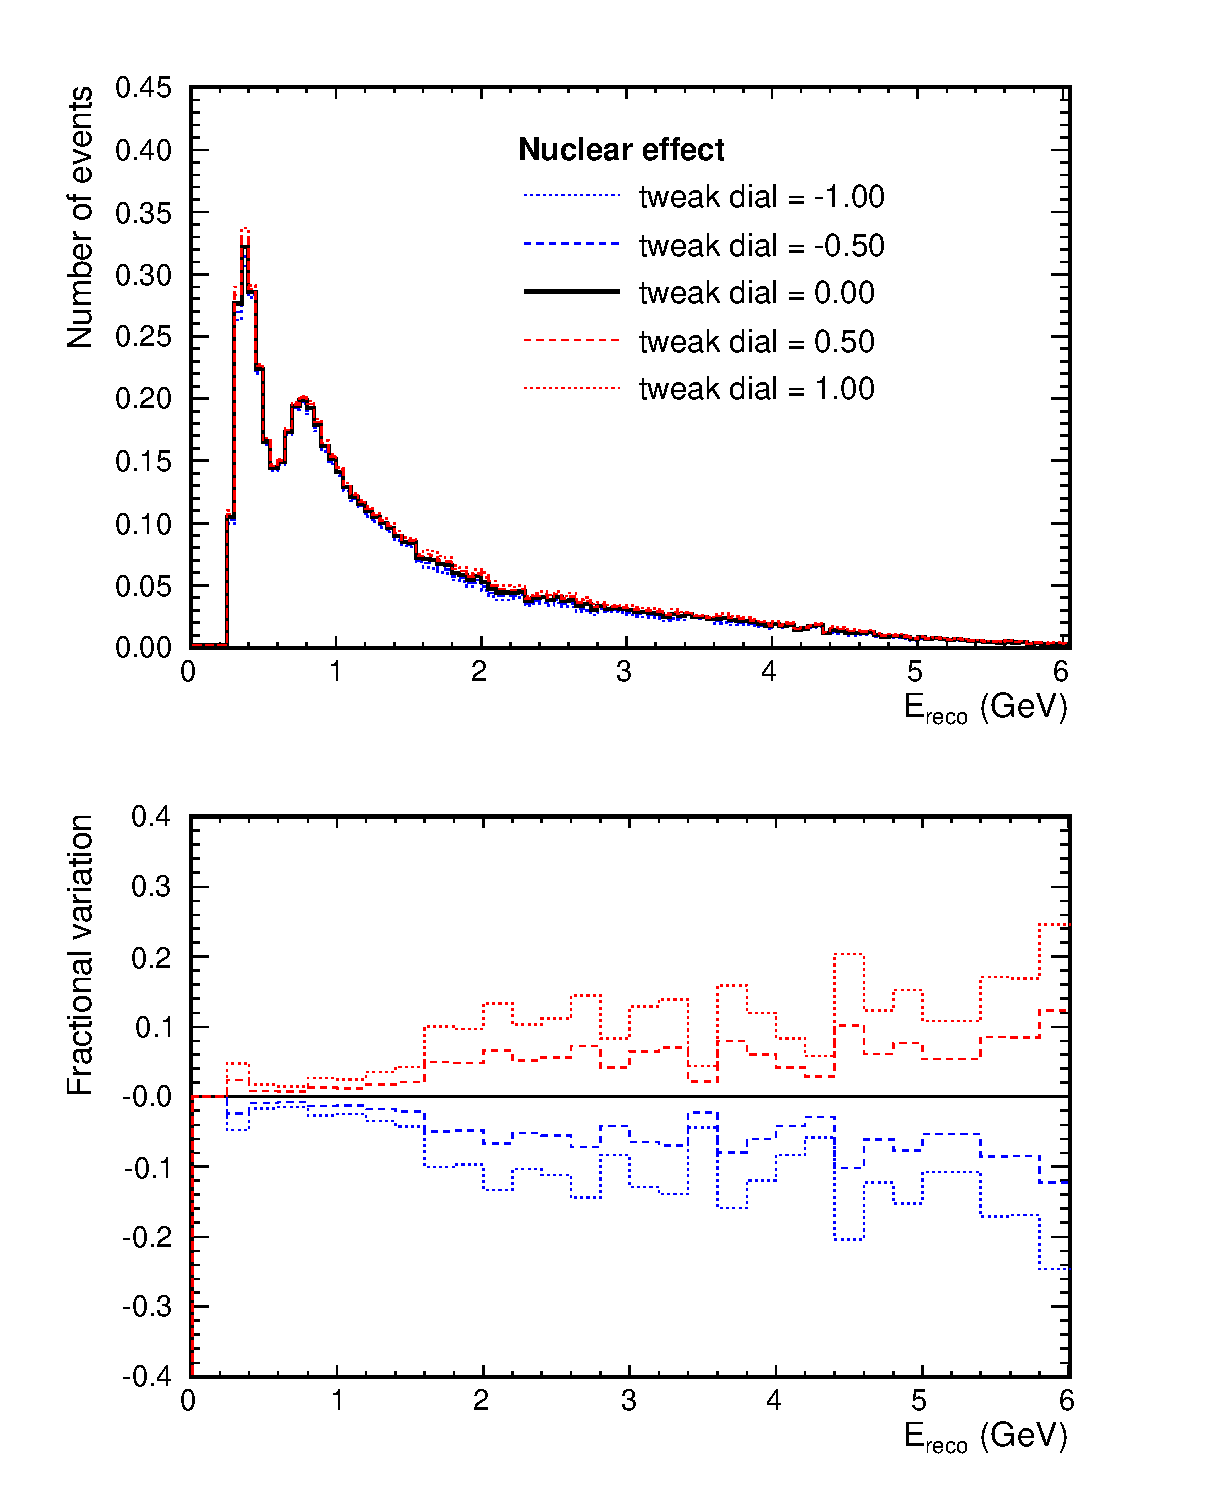
\includegraphics[width=19pc,height=21pc]{images/predicted_spectrum/systematic_variations/neut_sk_spectrum_twk_nuceff_2p4Em3_1p0.eps}
\caption{
  Effect of FSI variation to the NEUT
  reconstructed-energy spectrum of 1-ring muon-like events (after extrapolation).
  All spectra have oscillations with $sin^{2}2\theta_{23}$ = 1.0 and $\Delta m^{2}_{23}$ = 2.4$\times10^{-3}$ $eV^{2}/c^{4}$ applied.  
}
\label{fig:neut_sk_spectrum_twk_nuceff_2p4Em3_1p0}
\end{minipage}
\end{figure}

\clearpage

%
% ------------------------------------------------------------------------------------------
% GENIE TABLES
% ------------------------------------------------------------------------------------------
%

%
%
% SK CCQE efficiency: GENIE
%
%

\begin{table}
\centering
\begin{tabular}{| l | r | r  r | r  r |}
\hline
{\bf Component} &  {\bf Nominal}   &  \multicolumn {2}{c|} { {\bf +1$\sigma$} } &  \multicolumn {2}{c|} { {\bf -1$\sigma$} } \\
\hline
                                          $N_{SK}$ (1 $\mu$-like ring) &          6.2043 &          6.5019 &  4.80 \%  &          5.9066 & -4.80 \%  \\ 
\hline
                                             SK MC (1 $\mu$-like ring) &          5.3721 &          5.6299 &  4.80 \%  &          5.1144 & -4.80 \%  \\ 
\hline
                           SK MC (1 $\mu$-like ring): $\nu_{\mu}$ CCQE &          3.0985 &          3.3402 &  7.80 \%  &          2.8568 & -7.80 \%  \\ 
                       SK MC (1 $\mu$-like ring): $\nu_{\mu}$ CC1$\pi$ &          1.2545 &          1.2545 &  0.00 \%  &          1.2545 &  0.00 \%  \\ 
                       SK MC (1 $\mu$-like ring): $\nu_{\mu}$ CC other &          0.2177 &          0.2177 &  0.00 \%  &          0.2177 &  0.00 \%  \\ 
                         SK MC (1 $\mu$-like ring): $\nu_{\mu}$ CC all &          4.5707 &          4.8124 &  5.29 \%  &          4.3290 & -5.29 \%  \\ 
                         SK MC (1 $\mu$-like ring): $\nu_{\mu}$ NC all &          0.4087 &          0.4087 &  0.00 \%  &          0.4087 &  0.00 \%  \\ 
                     SK MC (1 $\mu$-like ring): $\bar{\nu_{\mu}}$ CCQE &          0.2056 &          0.2217 &  7.80 \%  &          0.1896 & -7.80 \%  \\ 
                 SK MC (1 $\mu$-like ring): $\bar{\nu_{\mu}}$ CC1$\pi$ &          0.1271 &          0.1271 &  0.00 \%  &          0.1271 &  0.00 \%  \\ 
                 SK MC (1 $\mu$-like ring): $\bar{\nu_{\mu}}$ CC other &          0.0215 &          0.0215 &  0.00 \%  &          0.0215 &  0.00 \%  \\ 
                   SK MC (1 $\mu$-like ring): $\bar{\nu_{\mu}}$ CC all &          0.3542 &          0.3702 &  4.53 \%  &          0.3382 & -4.53 \%  \\ 
                   SK MC (1 $\mu$-like ring): $\bar{\nu_{\mu}}$ NC all &          0.0236 &          0.0236 &  0.00 \%  &          0.0236 &  0.00 \%  \\ 
                             SK MC (1 $\mu$-like ring): $\nu_{e}$ CCQE &          0.0014 &          0.0014 &  0.00 \%  &          0.0014 &  0.00 \%  \\ 
                         SK MC (1 $\mu$-like ring): $\nu_{e}$ CC1$\pi$ &          0.0008 &          0.0008 &  0.00 \%  &          0.0008 &  0.00 \%  \\ 
                         SK MC (1 $\mu$-like ring): $\nu_{e}$ CC other &          0.0002 &          0.0002 &  0.00 \%  &          0.0002 &  0.00 \%  \\ 
                           SK MC (1 $\mu$-like ring): $\nu_{e}$ CC all &          0.0024 &          0.0024 &  0.00 \%  &          0.0024 &  0.00 \%  \\ 
                           SK MC (1 $\mu$-like ring): $\nu_{e}$ NC all &          0.0125 &          0.0125 &  0.00 \%  &          0.0125 &  0.00 \%  \\ 
\hline
                                       ND280 CC-like Observed/MC ratio &          1.1549 &          1.1549 &  0.00 \%  &          1.1549 &  0.00 \%  \\ 
                                                ND280 Observed CC-like &       1445.0000 &       1445.0000 &  0.00 \%  &       1445.0000 &  0.00 \%  \\ 
                                               ND280 MC: Total CC-like &       1251.1924 &       1251.1924 &  0.00 \%  &       1251.1924 &  0.00 \%  \\ 
                                                    ND280 MC: Total CC &       1199.6960 &       1199.6960 &  0.00 \%  &       1199.6960 &  0.00 \%  \\ 
                                         ND280 MC: Total NC background &         51.4964 &         51.4964 &  0.00 \%  &         51.4964 &  0.00 \%  \\ 
\hline
                                            ND280 MC: $\nu_{\mu}$ CCQE &        617.6298 &        617.6298 &  0.00 \%  &        617.6298 &  0.00 \%  \\ 
                                        ND280 MC: $\nu_{\mu}$ CC1$\pi$ &        291.9388 &        291.9388 &  0.00 \%  &        291.9388 &  0.00 \%  \\ 
                                        ND280 MC: $\nu_{\mu}$ CC other &        280.0197 &        280.0197 &  0.00 \%  &        280.0197 &  0.00 \%  \\ 
                                          ND280 MC: $\nu_{\mu}$ CC all &       1189.5883 &       1189.5883 &  0.00 \%  &       1189.5883 &  0.00 \%  \\ 
                                          ND280 MC: $\nu_{\mu}$ NC all &         48.8820 &         48.8820 &  0.00 \%  &         48.8820 &  0.00 \%  \\ 
                                      ND280 MC: $\bar{\nu_{\mu}}$ CCQE &          0.3815 &          0.3815 &  0.00 \%  &          0.3815 &  0.00 \%  \\ 
                                  ND280 MC: $\bar{\nu_{\mu}}$ CC1$\pi$ &          3.0898 &          3.0898 &  0.00 \%  &          3.0898 &  0.00 \%  \\ 
                                  ND280 MC: $\bar{\nu_{\mu}}$ CC other &          4.9767 &          4.9767 &  0.00 \%  &          4.9767 &  0.00 \%  \\ 
                                    ND280 MC: $\bar{\nu_{\mu}}$ CC all &          8.4480 &          8.4480 &  0.00 \%  &          8.4480 &  0.00 \%  \\ 
                                    ND280 MC: $\bar{\nu_{\mu}}$ NC all &          1.8276 &          1.8276 &  0.00 \%  &          1.8276 &  0.00 \%  \\ 
                                              ND280 MC: $\nu_{e}$ CCQE &          0.1889 &          0.1889 &  0.00 \%  &          0.1889 &  0.00 \%  \\ 
                                          ND280 MC: $\nu_{e}$ CC1$\pi$ &          0.4312 &          0.4312 &  0.00 \%  &          0.4312 &  0.00 \%  \\ 
                                          ND280 MC: $\nu_{e}$ CC other &          1.0397 &          1.0397 &  0.00 \%  &          1.0397 &  0.00 \%  \\ 
                                            ND280 MC: $\nu_{e}$ CC all &          1.6598 &          1.6598 &  0.00 \%  &          1.6598 &  0.00 \%  \\ 
                                            ND280 MC: $\nu_{e}$ NC all &          0.7868 &          0.7868 &  0.00 \%  &          0.7868 &  0.00 \%  \\ 
\hline
\end{tabular}
\caption{ 
  Effect of SuperK CCQE efficiency variation
  on various components of the oscillation analysis (GENIE).
  Oscillations with parameters $sin^{2}2\theta_{23}$ = 1.0 and $\Delta m^{2}_{23}$ = 2.4$\times10^{-3}$ $eV^{2}/c^{4}$ were applied.  
}
\label{tab:genie_sk_ccqe_eff}
\end{table}

%
%
% SK CCnonQE efficiency: GENIE
%
%

\begin{table}
\centering
\begin{tabular}{| l | r | r  r | r  r |}
\hline
{\bf Component} &  {\bf Nominal}   &  \multicolumn {2}{c|} { {\bf +1$\sigma$} } &  \multicolumn {2}{c|} { {\bf -1$\sigma$} } \\
\hline
                                          $N_{SK}$ (1 $\mu$-like ring) &          6.2043 &          6.6816 &  7.69 \%  &          5.7270 & -7.69 \%  \\ 
\hline
                                             SK MC (1 $\mu$-like ring) &          5.3721 &          5.7854 &  7.69 \%  &          4.9588 & -7.69 \%  \\ 
\hline
                           SK MC (1 $\mu$-like ring): $\nu_{\mu}$ CCQE &          3.0985 &          3.0985 &  0.00 \%  &          3.0985 &  0.00 \%  \\ 
                       SK MC (1 $\mu$-like ring): $\nu_{\mu}$ CC1$\pi$ &          1.2545 &          1.5744 & 25.50 \%  &          0.9346 & -25.50 \%  \\ 
                       SK MC (1 $\mu$-like ring): $\nu_{\mu}$ CC other &          0.2177 &          0.2732 & 25.50 \%  &          0.1622 & -25.50 \%  \\ 
                         SK MC (1 $\mu$-like ring): $\nu_{\mu}$ CC all &          4.5707 &          4.9461 &  8.21 \%  &          4.1953 & -8.21 \%  \\ 
                         SK MC (1 $\mu$-like ring): $\nu_{\mu}$ NC all &          0.4087 &          0.4087 &  0.00 \%  &          0.4087 &  0.00 \%  \\ 
                     SK MC (1 $\mu$-like ring): $\bar{\nu_{\mu}}$ CCQE &          0.2056 &          0.2056 &  0.00 \%  &          0.2056 &  0.00 \%  \\ 
                 SK MC (1 $\mu$-like ring): $\bar{\nu_{\mu}}$ CC1$\pi$ &          0.1271 &          0.1595 & 25.50 \%  &          0.0947 & -25.50 \%  \\ 
                 SK MC (1 $\mu$-like ring): $\bar{\nu_{\mu}}$ CC other &          0.0215 &          0.0270 & 25.50 \%  &          0.0160 & -25.50 \%  \\ 
                   SK MC (1 $\mu$-like ring): $\bar{\nu_{\mu}}$ CC all &          0.3542 &          0.3921 & 10.69 \%  &          0.3163 & -10.69 \%  \\ 
                   SK MC (1 $\mu$-like ring): $\bar{\nu_{\mu}}$ NC all &          0.0236 &          0.0236 &  0.00 \%  &          0.0236 &  0.00 \%  \\ 
                             SK MC (1 $\mu$-like ring): $\nu_{e}$ CCQE &          0.0014 &          0.0014 &  0.00 \%  &          0.0014 &  0.00 \%  \\ 
                         SK MC (1 $\mu$-like ring): $\nu_{e}$ CC1$\pi$ &          0.0008 &          0.0008 &  0.00 \%  &          0.0008 &  0.00 \%  \\ 
                         SK MC (1 $\mu$-like ring): $\nu_{e}$ CC other &          0.0002 &          0.0002 &  0.00 \%  &          0.0002 &  0.00 \%  \\ 
                           SK MC (1 $\mu$-like ring): $\nu_{e}$ CC all &          0.0024 &          0.0024 &  0.00 \%  &          0.0024 &  0.00 \%  \\ 
                           SK MC (1 $\mu$-like ring): $\nu_{e}$ NC all &          0.0125 &          0.0125 &  0.00 \%  &          0.0125 &  0.00 \%  \\ 
\hline
                                       ND280 CC-like Observed/MC ratio &          1.1549 &          1.1549 &  0.00 \%  &          1.1549 &  0.00 \%  \\ 
                                                ND280 Observed CC-like &       1445.0000 &       1445.0000 &  0.00 \%  &       1445.0000 &  0.00 \%  \\ 
                                               ND280 MC: Total CC-like &       1251.1924 &       1251.1924 &  0.00 \%  &       1251.1924 &  0.00 \%  \\ 
                                                    ND280 MC: Total CC &       1199.6960 &       1199.6960 &  0.00 \%  &       1199.6960 &  0.00 \%  \\ 
                                         ND280 MC: Total NC background &         51.4964 &         51.4964 &  0.00 \%  &         51.4964 &  0.00 \%  \\ 
\hline
                                            ND280 MC: $\nu_{\mu}$ CCQE &        617.6298 &        617.6298 &  0.00 \%  &        617.6298 &  0.00 \%  \\ 
                                        ND280 MC: $\nu_{\mu}$ CC1$\pi$ &        291.9388 &        291.9388 &  0.00 \%  &        291.9388 &  0.00 \%  \\ 
                                        ND280 MC: $\nu_{\mu}$ CC other &        280.0197 &        280.0197 &  0.00 \%  &        280.0197 &  0.00 \%  \\ 
                                          ND280 MC: $\nu_{\mu}$ CC all &       1189.5883 &       1189.5883 &  0.00 \%  &       1189.5883 &  0.00 \%  \\ 
                                          ND280 MC: $\nu_{\mu}$ NC all &         48.8820 &         48.8820 &  0.00 \%  &         48.8820 &  0.00 \%  \\ 
                                      ND280 MC: $\bar{\nu_{\mu}}$ CCQE &          0.3815 &          0.3815 &  0.00 \%  &          0.3815 &  0.00 \%  \\ 
                                  ND280 MC: $\bar{\nu_{\mu}}$ CC1$\pi$ &          3.0898 &          3.0898 &  0.00 \%  &          3.0898 &  0.00 \%  \\ 
                                  ND280 MC: $\bar{\nu_{\mu}}$ CC other &          4.9767 &          4.9767 &  0.00 \%  &          4.9767 &  0.00 \%  \\ 
                                    ND280 MC: $\bar{\nu_{\mu}}$ CC all &          8.4480 &          8.4480 &  0.00 \%  &          8.4480 &  0.00 \%  \\ 
                                    ND280 MC: $\bar{\nu_{\mu}}$ NC all &          1.8276 &          1.8276 &  0.00 \%  &          1.8276 &  0.00 \%  \\ 
                                              ND280 MC: $\nu_{e}$ CCQE &          0.1889 &          0.1889 &  0.00 \%  &          0.1889 &  0.00 \%  \\ 
                                          ND280 MC: $\nu_{e}$ CC1$\pi$ &          0.4312 &          0.4312 &  0.00 \%  &          0.4312 &  0.00 \%  \\ 
                                          ND280 MC: $\nu_{e}$ CC other &          1.0397 &          1.0397 &  0.00 \%  &          1.0397 &  0.00 \%  \\ 
                                            ND280 MC: $\nu_{e}$ CC all &          1.6598 &          1.6598 &  0.00 \%  &          1.6598 &  0.00 \%  \\ 
                                            ND280 MC: $\nu_{e}$ NC all &          0.7868 &          0.7868 &  0.00 \%  &          0.7868 &  0.00 \%  \\ 
\hline
\end{tabular}
\caption{ 
  Effect of SuperK CCnonQE efficiency variation
  on various components of the oscillation analysis (GENIE).
  Oscillations with parameters $sin^{2}2\theta_{23}$ = 1.0 and $\Delta m^{2}_{23}$ = 2.4$\times10^{-3}$ $eV^{2}/c^{4}$ were applied.  
}
\label{tab:genie_sk_ccnonqe_eff}
\end{table}

%
%
% SK NC efficiency: GENIE
%
%

\begin{table}
\centering
\begin{tabular}{| l | r | r  r | r  r |}
\hline
{\bf Component} &  {\bf Nominal}   &  \multicolumn {2}{c|} { {\bf +1$\sigma$} } &  \multicolumn {2}{c|} { {\bf -1$\sigma$} } \\
\hline
                                          $N_{SK}$ (1 $\mu$-like ring) &          6.2043 &          6.7956 &  9.53 \%  &          5.6130 & -9.53 \%  \\ 
\hline
                                             SK MC (1 $\mu$-like ring) &          5.3721 &          5.8841 &  9.53 \%  &          4.8601 & -9.53 \%  \\ 
\hline
                           SK MC (1 $\mu$-like ring): $\nu_{\mu}$ CCQE &          3.0985 &          3.0985 &  0.00 \%  &          3.0985 &  0.00 \%  \\ 
                       SK MC (1 $\mu$-like ring): $\nu_{\mu}$ CC1$\pi$ &          1.2545 &          1.2545 &  0.00 \%  &          1.2545 &  0.00 \%  \\ 
                       SK MC (1 $\mu$-like ring): $\nu_{\mu}$ CC other &          0.2177 &          0.2177 &  0.00 \%  &          0.2177 &  0.00 \%  \\ 
                         SK MC (1 $\mu$-like ring): $\nu_{\mu}$ CC all &          4.5707 &          4.5707 &  0.00 \%  &          4.5707 &  0.00 \%  \\ 
                         SK MC (1 $\mu$-like ring): $\nu_{\mu}$ NC all &          0.4087 &          0.8792 & 115.10 \%  &         -0.0617 & -115.10 \%  \\ 
                     SK MC (1 $\mu$-like ring): $\bar{\nu_{\mu}}$ CCQE &          0.2056 &          0.2056 &  0.00 \%  &          0.2056 &  0.00 \%  \\ 
                 SK MC (1 $\mu$-like ring): $\bar{\nu_{\mu}}$ CC1$\pi$ &          0.1271 &          0.1271 &  0.00 \%  &          0.1271 &  0.00 \%  \\ 
                 SK MC (1 $\mu$-like ring): $\bar{\nu_{\mu}}$ CC other &          0.0215 &          0.0215 &  0.00 \%  &          0.0215 &  0.00 \%  \\ 
                   SK MC (1 $\mu$-like ring): $\bar{\nu_{\mu}}$ CC all &          0.3542 &          0.3542 &  0.00 \%  &          0.3542 &  0.00 \%  \\ 
                   SK MC (1 $\mu$-like ring): $\bar{\nu_{\mu}}$ NC all &          0.0236 &          0.0509 & 115.10 \%  &         -0.0036 & -115.10 \%  \\ 
                             SK MC (1 $\mu$-like ring): $\nu_{e}$ CCQE &          0.0014 &          0.0014 &  0.00 \%  &          0.0014 &  0.00 \%  \\ 
                         SK MC (1 $\mu$-like ring): $\nu_{e}$ CC1$\pi$ &          0.0008 &          0.0008 &  0.00 \%  &          0.0008 &  0.00 \%  \\ 
                         SK MC (1 $\mu$-like ring): $\nu_{e}$ CC other &          0.0002 &          0.0002 &  0.00 \%  &          0.0002 &  0.00 \%  \\ 
                           SK MC (1 $\mu$-like ring): $\nu_{e}$ CC all &          0.0024 &          0.0024 &  0.00 \%  &          0.0024 &  0.00 \%  \\ 
                           SK MC (1 $\mu$-like ring): $\nu_{e}$ NC all &          0.0125 &          0.0268 & 115.10 \%  &         -0.0019 & -115.10 \%  \\ 
\hline
                                       ND280 CC-like Observed/MC ratio &          1.1549 &          1.1549 &  0.00 \%  &          1.1549 &  0.00 \%  \\ 
                                                ND280 Observed CC-like &       1445.0000 &       1445.0000 &  0.00 \%  &       1445.0000 &  0.00 \%  \\ 
                                               ND280 MC: Total CC-like &       1251.1924 &       1251.1924 &  0.00 \%  &       1251.1924 &  0.00 \%  \\ 
                                                    ND280 MC: Total CC &       1199.6960 &       1199.6960 &  0.00 \%  &       1199.6960 &  0.00 \%  \\ 
                                         ND280 MC: Total NC background &         51.4964 &         51.4964 &  0.00 \%  &         51.4964 &  0.00 \%  \\ 
\hline
                                            ND280 MC: $\nu_{\mu}$ CCQE &        617.6298 &        617.6298 &  0.00 \%  &        617.6298 &  0.00 \%  \\ 
                                        ND280 MC: $\nu_{\mu}$ CC1$\pi$ &        291.9388 &        291.9388 &  0.00 \%  &        291.9388 &  0.00 \%  \\ 
                                        ND280 MC: $\nu_{\mu}$ CC other &        280.0197 &        280.0197 &  0.00 \%  &        280.0197 &  0.00 \%  \\ 
                                          ND280 MC: $\nu_{\mu}$ CC all &       1189.5883 &       1189.5883 &  0.00 \%  &       1189.5883 &  0.00 \%  \\ 
                                          ND280 MC: $\nu_{\mu}$ NC all &         48.8820 &         48.8820 &  0.00 \%  &         48.8820 &  0.00 \%  \\ 
                                      ND280 MC: $\bar{\nu_{\mu}}$ CCQE &          0.3815 &          0.3815 &  0.00 \%  &          0.3815 &  0.00 \%  \\ 
                                  ND280 MC: $\bar{\nu_{\mu}}$ CC1$\pi$ &          3.0898 &          3.0898 &  0.00 \%  &          3.0898 &  0.00 \%  \\ 
                                  ND280 MC: $\bar{\nu_{\mu}}$ CC other &          4.9767 &          4.9767 &  0.00 \%  &          4.9767 &  0.00 \%  \\ 
                                    ND280 MC: $\bar{\nu_{\mu}}$ CC all &          8.4480 &          8.4480 &  0.00 \%  &          8.4480 &  0.00 \%  \\ 
                                    ND280 MC: $\bar{\nu_{\mu}}$ NC all &          1.8276 &          1.8276 &  0.00 \%  &          1.8276 &  0.00 \%  \\ 
                                              ND280 MC: $\nu_{e}$ CCQE &          0.1889 &          0.1889 &  0.00 \%  &          0.1889 &  0.00 \%  \\ 
                                          ND280 MC: $\nu_{e}$ CC1$\pi$ &          0.4312 &          0.4312 &  0.00 \%  &          0.4312 &  0.00 \%  \\ 
                                          ND280 MC: $\nu_{e}$ CC other &          1.0397 &          1.0397 &  0.00 \%  &          1.0397 &  0.00 \%  \\ 
                                            ND280 MC: $\nu_{e}$ CC all &          1.6598 &          1.6598 &  0.00 \%  &          1.6598 &  0.00 \%  \\ 
                                            ND280 MC: $\nu_{e}$ NC all &          0.7868 &          0.7868 &  0.00 \%  &          0.7868 &  0.00 \%  \\ 
\hline
\end{tabular}
\caption{ 
  Effect of SuperK NC efficiency variation
  on various components of the oscillation analysis (GENIE).
  Oscillations with parameters $sin^{2}2\theta_{23}$ = 1.0 and $\Delta m^{2}_{23}$ = 2.4$\times10^{-3}$ $eV^{2}/c^{4}$ were applied.  
}
\label{tab:genie_sk_nc_eff}
\end{table}


%
%
% SK nue CC efficiency: GENIE
%
%


\begin{table}
\centering
\begin{tabular}{| l | r | r  r | r  r |}
\hline
{\bf Component} &  {\bf Nominal}   &  \multicolumn {2}{c|} { {\bf +1$\sigma$} } &  \multicolumn {2}{c|} { {\bf -1$\sigma$} } \\
\hline
                                          $N_{SK}$ (1 $\mu$-like ring) &          6.2043 &          6.2071 &  0.05 \%  &          6.2015 & -0.05 \%  \\ 
\hline
                                             SK MC (1 $\mu$-like ring) &          5.3721 &          5.3745 &  0.05 \%  &          5.3697 & -0.05 \%  \\ 
\hline
                           SK MC (1 $\mu$-like ring): $\nu_{\mu}$ CCQE &          3.0985 &          3.0985 &  0.00 \%  &          3.0985 &  0.00 \%  \\ 
                       SK MC (1 $\mu$-like ring): $\nu_{\mu}$ CC1$\pi$ &          1.2545 &          1.2545 &  0.00 \%  &          1.2545 &  0.00 \%  \\ 
                       SK MC (1 $\mu$-like ring): $\nu_{\mu}$ CC other &          0.2177 &          0.2177 &  0.00 \%  &          0.2177 &  0.00 \%  \\ 
                         SK MC (1 $\mu$-like ring): $\nu_{\mu}$ CC all &          4.5707 &          4.5707 &  0.00 \%  &          4.5707 &  0.00 \%  \\ 
                         SK MC (1 $\mu$-like ring): $\nu_{\mu}$ NC all &          0.4087 &          0.4087 &  0.00 \%  &          0.4087 &  0.00 \%  \\ 
                     SK MC (1 $\mu$-like ring): $\bar{\nu_{\mu}}$ CCQE &          0.2056 &          0.2056 &  0.00 \%  &          0.2056 &  0.00 \%  \\ 
                 SK MC (1 $\mu$-like ring): $\bar{\nu_{\mu}}$ CC1$\pi$ &          0.1271 &          0.1271 &  0.00 \%  &          0.1271 &  0.00 \%  \\ 
                 SK MC (1 $\mu$-like ring): $\bar{\nu_{\mu}}$ CC other &          0.0215 &          0.0215 &  0.00 \%  &          0.0215 &  0.00 \%  \\ 
                   SK MC (1 $\mu$-like ring): $\bar{\nu_{\mu}}$ CC all &          0.3542 &          0.3542 &  0.00 \%  &          0.3542 &  0.00 \%  \\ 
                   SK MC (1 $\mu$-like ring): $\bar{\nu_{\mu}}$ NC all &          0.0236 &          0.0236 &  0.00 \%  &          0.0236 &  0.00 \%  \\ 
                             SK MC (1 $\mu$-like ring): $\nu_{e}$ CCQE &          0.0014 &          0.0027 & 100.00 \%  &          0.0000 & -100.00 \%  \\ 
                         SK MC (1 $\mu$-like ring): $\nu_{e}$ CC1$\pi$ &          0.0008 &          0.0016 & 100.00 \%  &          0.0000 & -100.00 \%  \\ 
                         SK MC (1 $\mu$-like ring): $\nu_{e}$ CC other &          0.0002 &          0.0005 & 100.00 \%  &          0.0000 & -100.00 \%  \\ 
                           SK MC (1 $\mu$-like ring): $\nu_{e}$ CC all &          0.0024 &          0.0048 & 100.00 \%  &          0.0000 & -100.00 \%  \\ 
                           SK MC (1 $\mu$-like ring): $\nu_{e}$ NC all &          0.0125 &          0.0125 &  0.00 \%  &          0.0125 &  0.00 \%  \\ 
\hline
                                       ND280 CC-like Observed/MC ratio &          1.1549 &          1.1549 &  0.00 \%  &          1.1549 &  0.00 \%  \\ 
                                                ND280 Observed CC-like &       1445.0000 &       1445.0000 &  0.00 \%  &       1445.0000 &  0.00 \%  \\ 
                                               ND280 MC: Total CC-like &       1251.1924 &       1251.1924 &  0.00 \%  &       1251.1924 &  0.00 \%  \\ 
                                                    ND280 MC: Total CC &       1199.6960 &       1199.6960 &  0.00 \%  &       1199.6960 &  0.00 \%  \\ 
                                         ND280 MC: Total NC background &         51.4964 &         51.4964 &  0.00 \%  &         51.4964 &  0.00 \%  \\ 
\hline
                                            ND280 MC: $\nu_{\mu}$ CCQE &        617.6298 &        617.6298 &  0.00 \%  &        617.6298 &  0.00 \%  \\ 
                                        ND280 MC: $\nu_{\mu}$ CC1$\pi$ &        291.9388 &        291.9388 &  0.00 \%  &        291.9388 &  0.00 \%  \\ 
                                        ND280 MC: $\nu_{\mu}$ CC other &        280.0197 &        280.0197 &  0.00 \%  &        280.0197 &  0.00 \%  \\ 
                                          ND280 MC: $\nu_{\mu}$ CC all &       1189.5883 &       1189.5883 &  0.00 \%  &       1189.5883 &  0.00 \%  \\ 
                                          ND280 MC: $\nu_{\mu}$ NC all &         48.8820 &         48.8820 &  0.00 \%  &         48.8820 &  0.00 \%  \\ 
                                      ND280 MC: $\bar{\nu_{\mu}}$ CCQE &          0.3815 &          0.3815 &  0.00 \%  &          0.3815 &  0.00 \%  \\ 
                                  ND280 MC: $\bar{\nu_{\mu}}$ CC1$\pi$ &          3.0898 &          3.0898 &  0.00 \%  &          3.0898 &  0.00 \%  \\ 
                                  ND280 MC: $\bar{\nu_{\mu}}$ CC other &          4.9767 &          4.9767 &  0.00 \%  &          4.9767 &  0.00 \%  \\ 
                                    ND280 MC: $\bar{\nu_{\mu}}$ CC all &          8.4480 &          8.4480 &  0.00 \%  &          8.4480 &  0.00 \%  \\ 
                                    ND280 MC: $\bar{\nu_{\mu}}$ NC all &          1.8276 &          1.8276 &  0.00 \%  &          1.8276 &  0.00 \%  \\ 
                                              ND280 MC: $\nu_{e}$ CCQE &          0.1889 &          0.1889 &  0.00 \%  &          0.1889 &  0.00 \%  \\ 
                                          ND280 MC: $\nu_{e}$ CC1$\pi$ &          0.4312 &          0.4312 &  0.00 \%  &          0.4312 &  0.00 \%  \\ 
                                          ND280 MC: $\nu_{e}$ CC other &          1.0397 &          1.0397 &  0.00 \%  &          1.0397 &  0.00 \%  \\ 
                                            ND280 MC: $\nu_{e}$ CC all &          1.6598 &          1.6598 &  0.00 \%  &          1.6598 &  0.00 \%  \\ 
                                            ND280 MC: $\nu_{e}$ NC all &          0.7868 &          0.7868 &  0.00 \%  &          0.7868 &  0.00 \%  \\ 
\hline
\end{tabular}
\caption{ 
  Effect of SuperK $\nu_{e} CC$ efficiency variation
  on various components of the oscillation analysis (GENIE).
  Oscillations with parameters $sin^{2}2\theta_{23}$ = 1.0 and $\Delta m^{2}_{23}$ = 2.4$\times10^{-3}$ $eV^{2}/c^{4}$ were applied.  
}
\label{tab:genie_sk_nuecc_eff}
\end{table}


%
%
% ND280 efficiency: GENIE
%
%

\begin{table}
\centering
\begin{tabular}{| l | r | r  r | r  r |}
\hline
{\bf Component} &  {\bf Nominal}   &  \multicolumn {2}{c|} { {\bf +1$\sigma$} } &  \multicolumn {2}{c|} { {\bf -1$\sigma$} } \\
\hline
                                          $N_{SK}$ (1 $\mu$-like ring) &          6.2043 &          5.9088 & -4.76 \%  &          6.5308 &  5.26 \%  \\ 
\hline
                                             SK MC (1 $\mu$-like ring) &          5.3721 &          5.3721 &  0.00 \%  &          5.3721 &  0.00 \%  \\ 
\hline
                           SK MC (1 $\mu$-like ring): $\nu_{\mu}$ CCQE &          3.0985 &          3.0985 &  0.00 \%  &          3.0985 &  0.00 \%  \\ 
                       SK MC (1 $\mu$-like ring): $\nu_{\mu}$ CC1$\pi$ &          1.2545 &          1.2545 &  0.00 \%  &          1.2545 &  0.00 \%  \\ 
                       SK MC (1 $\mu$-like ring): $\nu_{\mu}$ CC other &          0.2177 &          0.2177 &  0.00 \%  &          0.2177 &  0.00 \%  \\ 
                         SK MC (1 $\mu$-like ring): $\nu_{\mu}$ CC all &          4.5707 &          4.5707 &  0.00 \%  &          4.5707 &  0.00 \%  \\ 
                         SK MC (1 $\mu$-like ring): $\nu_{\mu}$ NC all &          0.4087 &          0.4087 &  0.00 \%  &          0.4087 &  0.00 \%  \\ 
                     SK MC (1 $\mu$-like ring): $\bar{\nu_{\mu}}$ CCQE &          0.2056 &          0.2056 &  0.00 \%  &          0.2056 &  0.00 \%  \\ 
                 SK MC (1 $\mu$-like ring): $\bar{\nu_{\mu}}$ CC1$\pi$ &          0.1271 &          0.1271 &  0.00 \%  &          0.1271 &  0.00 \%  \\ 
                 SK MC (1 $\mu$-like ring): $\bar{\nu_{\mu}}$ CC other &          0.0215 &          0.0215 &  0.00 \%  &          0.0215 &  0.00 \%  \\ 
                   SK MC (1 $\mu$-like ring): $\bar{\nu_{\mu}}$ CC all &          0.3542 &          0.3542 &  0.00 \%  &          0.3542 &  0.00 \%  \\ 
                   SK MC (1 $\mu$-like ring): $\bar{\nu_{\mu}}$ NC all &          0.0236 &          0.0236 &  0.00 \%  &          0.0236 &  0.00 \%  \\ 
                             SK MC (1 $\mu$-like ring): $\nu_{e}$ CCQE &          0.0014 &          0.0014 &  0.00 \%  &          0.0014 &  0.00 \%  \\ 
                         SK MC (1 $\mu$-like ring): $\nu_{e}$ CC1$\pi$ &          0.0008 &          0.0008 &  0.00 \%  &          0.0008 &  0.00 \%  \\ 
                         SK MC (1 $\mu$-like ring): $\nu_{e}$ CC other &          0.0002 &          0.0002 &  0.00 \%  &          0.0002 &  0.00 \%  \\ 
                           SK MC (1 $\mu$-like ring): $\nu_{e}$ CC all &          0.0024 &          0.0024 &  0.00 \%  &          0.0024 &  0.00 \%  \\ 
                           SK MC (1 $\mu$-like ring): $\nu_{e}$ NC all &          0.0125 &          0.0125 &  0.00 \%  &          0.0125 &  0.00 \%  \\ 
\hline
                                       ND280 CC-like Observed/MC ratio &          1.1549 &          1.0999 & -4.76 \%  &          1.2157 &  5.26 \%  \\ 
                                                ND280 Observed CC-like &       1445.0000 &       1445.0000 &  0.00 \%  &       1445.0000 &  0.00 \%  \\ 
                                               ND280 MC: Total CC-like &       1251.1924 &       1313.7520 &  5.00 \%  &       1188.6327 & -5.00 \%  \\ 
                                                    ND280 MC: Total CC &       1199.6960 &       1259.6808 &  5.00 \%  &       1139.7112 & -5.00 \%  \\ 
                                         ND280 MC: Total NC background &         51.4964 &         54.0712 &  5.00 \%  &         48.9215 & -5.00 \%  \\ 
\hline
                                            ND280 MC: $\nu_{\mu}$ CCQE &        617.6298 &        648.5112 &  5.00 \%  &        586.7483 & -5.00 \%  \\ 
                                        ND280 MC: $\nu_{\mu}$ CC1$\pi$ &        291.9388 &        306.5358 &  5.00 \%  &        277.3419 & -5.00 \%  \\ 
                                        ND280 MC: $\nu_{\mu}$ CC other &        280.0197 &        294.0206 &  5.00 \%  &        266.0187 & -5.00 \%  \\ 
                                          ND280 MC: $\nu_{\mu}$ CC all &       1189.5883 &       1249.0677 &  5.00 \%  &       1130.1088 & -5.00 \%  \\ 
                                          ND280 MC: $\nu_{\mu}$ NC all &         48.8820 &         51.3261 &  5.00 \%  &         46.4379 & -5.00 \%  \\ 
                                      ND280 MC: $\bar{\nu_{\mu}}$ CCQE &          0.3815 &          0.4006 &  5.00 \%  &          0.3624 & -5.00 \%  \\ 
                                  ND280 MC: $\bar{\nu_{\mu}}$ CC1$\pi$ &          3.0898 &          3.2443 &  5.00 \%  &          2.9353 & -5.00 \%  \\ 
                                  ND280 MC: $\bar{\nu_{\mu}}$ CC other &          4.9767 &          5.2255 &  5.00 \%  &          4.7278 & -5.00 \%  \\ 
                                    ND280 MC: $\bar{\nu_{\mu}}$ CC all &          8.4480 &          8.8704 &  5.00 \%  &          8.0256 & -5.00 \%  \\ 
                                    ND280 MC: $\bar{\nu_{\mu}}$ NC all &          1.8276 &          1.9190 &  5.00 \%  &          1.7362 & -5.00 \%  \\ 
                                              ND280 MC: $\nu_{e}$ CCQE &          0.1889 &          0.1983 &  5.00 \%  &          0.1794 & -5.00 \%  \\ 
                                          ND280 MC: $\nu_{e}$ CC1$\pi$ &          0.4312 &          0.4528 &  5.00 \%  &          0.4097 & -5.00 \%  \\ 
                                          ND280 MC: $\nu_{e}$ CC other &          1.0397 &          1.0917 &  5.00 \%  &          0.9877 & -5.00 \%  \\ 
                                            ND280 MC: $\nu_{e}$ CC all &          1.6598 &          1.7427 &  5.00 \%  &          1.5768 & -5.00 \%  \\ 
                                            ND280 MC: $\nu_{e}$ NC all &          0.7868 &          0.8262 &  5.00 \%  &          0.7475 & -5.00 \%  \\ 
\hline
\end{tabular}
\caption{ 
  Effect of ND280 efficiency variation
  on various components of the oscillation analysis (GENIE).
  Oscillations with parameters $sin^{2}2\theta_{23}$ = 1.0 and $\Delta m^{2}_{23}$ = 2.4$\times10^{-3}$ $eV^{2}/c^{4}$ were applied.  
}
\label{tab:genie_nd280_eff}
\end{table}


%
%
% Beam norm: GENIE
%
%

\begin{table}
\centering
\begin{tabular}{| l | r | r  r | r  r |}
\hline
{\bf Component} &  {\bf Nominal}   &  \multicolumn {2}{c|} { {\bf +1$\sigma$} } &  \multicolumn {2}{c|} { {\bf -1$\sigma$} } \\
\hline
                                          $N_{SK}$ (1 $\mu$-like ring) &          6.2043 &          6.6112 &  6.56 \%  &          5.7973 & -6.56 \%  \\ 
\hline
                                             SK MC (1 $\mu$-like ring) &          5.3721 &          5.3721 &  0.00 \%  &          5.3721 &  0.00 \%  \\ 
\hline
                           SK MC (1 $\mu$-like ring): $\nu_{\mu}$ CCQE &          3.0985 &          3.0985 &  0.00 \%  &          3.0985 &  0.00 \%  \\ 
                       SK MC (1 $\mu$-like ring): $\nu_{\mu}$ CC1$\pi$ &          1.2545 &          1.2545 &  0.00 \%  &          1.2545 &  0.00 \%  \\ 
                       SK MC (1 $\mu$-like ring): $\nu_{\mu}$ CC other &          0.2177 &          0.2177 &  0.00 \%  &          0.2177 &  0.00 \%  \\ 
                         SK MC (1 $\mu$-like ring): $\nu_{\mu}$ CC all &          4.5707 &          4.5707 &  0.00 \%  &          4.5707 &  0.00 \%  \\ 
                         SK MC (1 $\mu$-like ring): $\nu_{\mu}$ NC all &          0.4087 &          0.4087 &  0.00 \%  &          0.4087 &  0.00 \%  \\ 
                     SK MC (1 $\mu$-like ring): $\bar{\nu_{\mu}}$ CCQE &          0.2056 &          0.2056 &  0.00 \%  &          0.2056 &  0.00 \%  \\ 
                 SK MC (1 $\mu$-like ring): $\bar{\nu_{\mu}}$ CC1$\pi$ &          0.1271 &          0.1271 &  0.00 \%  &          0.1271 &  0.00 \%  \\ 
                 SK MC (1 $\mu$-like ring): $\bar{\nu_{\mu}}$ CC other &          0.0215 &          0.0215 &  0.00 \%  &          0.0215 &  0.00 \%  \\ 
                   SK MC (1 $\mu$-like ring): $\bar{\nu_{\mu}}$ CC all &          0.3542 &          0.3542 &  0.00 \%  &          0.3542 &  0.00 \%  \\ 
                   SK MC (1 $\mu$-like ring): $\bar{\nu_{\mu}}$ NC all &          0.0236 &          0.0236 &  0.00 \%  &          0.0236 &  0.00 \%  \\ 
                             SK MC (1 $\mu$-like ring): $\nu_{e}$ CCQE &          0.0014 &          0.0014 &  0.00 \%  &          0.0014 &  0.00 \%  \\ 
                         SK MC (1 $\mu$-like ring): $\nu_{e}$ CC1$\pi$ &          0.0008 &          0.0008 &  0.00 \%  &          0.0008 &  0.00 \%  \\ 
                         SK MC (1 $\mu$-like ring): $\nu_{e}$ CC other &          0.0002 &          0.0002 &  0.00 \%  &          0.0002 &  0.00 \%  \\ 
                           SK MC (1 $\mu$-like ring): $\nu_{e}$ CC all &          0.0024 &          0.0024 &  0.00 \%  &          0.0024 &  0.00 \%  \\ 
                           SK MC (1 $\mu$-like ring): $\nu_{e}$ NC all &          0.0125 &          0.0125 &  0.00 \%  &          0.0125 &  0.00 \%  \\ 
\hline
                                       ND280 CC-like Observed/MC ratio &          1.1549 &          1.1549 &  0.00 \%  &          1.1549 &  0.00 \%  \\ 
                                                ND280 Observed CC-like &       1445.0000 &       1445.0000 &  0.00 \%  &       1445.0000 &  0.00 \%  \\ 
                                               ND280 MC: Total CC-like &       1251.1924 &       1251.1924 &  0.00 \%  &       1251.1924 &  0.00 \%  \\ 
                                                    ND280 MC: Total CC &       1199.6960 &       1199.6960 &  0.00 \%  &       1199.6960 &  0.00 \%  \\ 
                                         ND280 MC: Total NC background &         51.4964 &         51.4964 &  0.00 \%  &         51.4964 &  0.00 \%  \\ 
\hline
                                            ND280 MC: $\nu_{\mu}$ CCQE &        617.6298 &        617.6298 &  0.00 \%  &        617.6298 &  0.00 \%  \\ 
                                        ND280 MC: $\nu_{\mu}$ CC1$\pi$ &        291.9388 &        291.9388 &  0.00 \%  &        291.9388 &  0.00 \%  \\ 
                                        ND280 MC: $\nu_{\mu}$ CC other &        280.0197 &        280.0197 &  0.00 \%  &        280.0197 &  0.00 \%  \\ 
                                          ND280 MC: $\nu_{\mu}$ CC all &       1189.5883 &       1189.5883 &  0.00 \%  &       1189.5883 &  0.00 \%  \\ 
                                          ND280 MC: $\nu_{\mu}$ NC all &         48.8820 &         48.8820 &  0.00 \%  &         48.8820 &  0.00 \%  \\ 
                                      ND280 MC: $\bar{\nu_{\mu}}$ CCQE &          0.3815 &          0.3815 &  0.00 \%  &          0.3815 &  0.00 \%  \\ 
                                  ND280 MC: $\bar{\nu_{\mu}}$ CC1$\pi$ &          3.0898 &          3.0898 &  0.00 \%  &          3.0898 &  0.00 \%  \\ 
                                  ND280 MC: $\bar{\nu_{\mu}}$ CC other &          4.9767 &          4.9767 &  0.00 \%  &          4.9767 &  0.00 \%  \\ 
                                    ND280 MC: $\bar{\nu_{\mu}}$ CC all &          8.4480 &          8.4480 &  0.00 \%  &          8.4480 &  0.00 \%  \\ 
                                    ND280 MC: $\bar{\nu_{\mu}}$ NC all &          1.8276 &          1.8276 &  0.00 \%  &          1.8276 &  0.00 \%  \\ 
                                              ND280 MC: $\nu_{e}$ CCQE &          0.1889 &          0.1889 &  0.00 \%  &          0.1889 &  0.00 \%  \\ 
                                          ND280 MC: $\nu_{e}$ CC1$\pi$ &          0.4312 &          0.4312 &  0.00 \%  &          0.4312 &  0.00 \%  \\ 
                                          ND280 MC: $\nu_{e}$ CC other &          1.0397 &          1.0397 &  0.00 \%  &          1.0397 &  0.00 \%  \\ 
                                            ND280 MC: $\nu_{e}$ CC all &          1.6598 &          1.6598 &  0.00 \%  &          1.6598 &  0.00 \%  \\ 
                                            ND280 MC: $\nu_{e}$ NC all &          0.7868 &          0.7868 &  0.00 \%  &          0.7868 &  0.00 \%  \\ 
\hline
\end{tabular}
\caption{ 
  Effect of flux normalization variation
  on various components of the oscillation analysis (GENIE).
  Oscillations with parameters $sin^{2}2\theta_{23}$ = 1.0 and $\Delta m^{2}_{23}$ = 2.4$\times10^{-3}$ $eV^{2}/c^{4}$ were applied.  
}
\label{tab:genie_flux_norm}
\end{table}


%
%
% CCQE cross section: GENIE
%
%

\begin{table}
\centering
\begin{tabular}{| l | r | r  r | r  r |}
\hline
{\bf Component} &  {\bf Nominal}   &  \multicolumn {2}{c|} { {\bf +1$\sigma$} } &  \multicolumn {2}{c|} { {\bf -1$\sigma$} } \\
\hline
                                          $N_{SK}$ (1 $\mu$-like ring) &          6.2043 &          6.3896 &  2.99 \%  &          6.0189 & -2.99 \%  \\ 
\hline
                                             SK MC (1 $\mu$-like ring) &          5.3721 &          5.5326 &  2.99 \%  &          5.2117 & -2.99 \%  \\ 
\hline
                           SK MC (1 $\mu$-like ring): $\nu_{\mu}$ CCQE &          3.0985 &          3.2545 &  5.04 \%  &          2.9425 & -5.04 \%  \\ 
                       SK MC (1 $\mu$-like ring): $\nu_{\mu}$ CC1$\pi$ &          1.2545 &          1.2545 &  0.00 \%  &          1.2545 &  0.00 \%  \\ 
                       SK MC (1 $\mu$-like ring): $\nu_{\mu}$ CC other &          0.2177 &          0.2177 &  0.00 \%  &          0.2177 &  0.00 \%  \\ 
                         SK MC (1 $\mu$-like ring): $\nu_{\mu}$ CC all &          4.5707 &          4.7267 &  3.41 \%  &          4.4147 & -3.41 \%  \\ 
                         SK MC (1 $\mu$-like ring): $\nu_{\mu}$ NC all &          0.4087 &          0.4087 &  0.00 \%  &          0.4087 &  0.00 \%  \\ 
                     SK MC (1 $\mu$-like ring): $\bar{\nu_{\mu}}$ CCQE &          0.2056 &          0.2100 &  2.11 \%  &          0.2013 & -2.11 \%  \\ 
                 SK MC (1 $\mu$-like ring): $\bar{\nu_{\mu}}$ CC1$\pi$ &          0.1271 &          0.1271 &  0.00 \%  &          0.1271 &  0.00 \%  \\ 
                 SK MC (1 $\mu$-like ring): $\bar{\nu_{\mu}}$ CC other &          0.0215 &          0.0215 &  0.00 \%  &          0.0215 &  0.00 \%  \\ 
                   SK MC (1 $\mu$-like ring): $\bar{\nu_{\mu}}$ CC all &          0.3542 &          0.3585 &  1.23 \%  &          0.3499 & -1.23 \%  \\ 
                   SK MC (1 $\mu$-like ring): $\bar{\nu_{\mu}}$ NC all &          0.0236 &          0.0236 &  0.00 \%  &          0.0236 &  0.00 \%  \\ 
                             SK MC (1 $\mu$-like ring): $\nu_{e}$ CCQE &          0.0014 &          0.0015 &  6.79 \%  &          0.0013 & -6.79 \%  \\ 
                         SK MC (1 $\mu$-like ring): $\nu_{e}$ CC1$\pi$ &          0.0008 &          0.0008 &  0.00 \%  &          0.0008 &  0.00 \%  \\ 
                         SK MC (1 $\mu$-like ring): $\nu_{e}$ CC other &          0.0002 &          0.0002 &  0.00 \%  &          0.0002 &  0.00 \%  \\ 
                           SK MC (1 $\mu$-like ring): $\nu_{e}$ CC all &          0.0024 &          0.0025 &  3.85 \%  &          0.0023 & -3.85 \%  \\ 
                           SK MC (1 $\mu$-like ring): $\nu_{e}$ NC all &          0.0125 &          0.0125 &  0.00 \%  &          0.0125 &  0.00 \%  \\ 
\hline
                                       ND280 CC-like Observed/MC ratio &          1.1549 &          1.1549 &  0.00 \%  &          1.1549 &  0.00 \%  \\ 
                                                ND280 Observed CC-like &       1445.0000 &       1445.0000 &  0.00 \%  &       1445.0000 &  0.00 \%  \\ 
                                               ND280 MC: Total CC-like &       1251.1924 &       1251.1924 &  0.00 \%  &       1251.1924 &  0.00 \%  \\ 
                                                    ND280 MC: Total CC &       1199.6960 &       1199.6960 &  0.00 \%  &       1199.6960 &  0.00 \%  \\ 
                                         ND280 MC: Total NC background &         51.4964 &         51.4964 &  0.00 \%  &         51.4964 &  0.00 \%  \\ 
\hline
                                            ND280 MC: $\nu_{\mu}$ CCQE &        617.6298 &        617.6298 &  0.00 \%  &        617.6298 &  0.00 \%  \\ 
                                        ND280 MC: $\nu_{\mu}$ CC1$\pi$ &        291.9388 &        291.9388 &  0.00 \%  &        291.9388 &  0.00 \%  \\ 
                                        ND280 MC: $\nu_{\mu}$ CC other &        280.0197 &        280.0197 &  0.00 \%  &        280.0197 &  0.00 \%  \\ 
                                          ND280 MC: $\nu_{\mu}$ CC all &       1189.5883 &       1189.5883 &  0.00 \%  &       1189.5883 &  0.00 \%  \\ 
                                          ND280 MC: $\nu_{\mu}$ NC all &         48.8820 &         48.8820 &  0.00 \%  &         48.8820 &  0.00 \%  \\ 
                                      ND280 MC: $\bar{\nu_{\mu}}$ CCQE &          0.3815 &          0.3815 &  0.00 \%  &          0.3815 &  0.00 \%  \\ 
                                  ND280 MC: $\bar{\nu_{\mu}}$ CC1$\pi$ &          3.0898 &          3.0898 &  0.00 \%  &          3.0898 &  0.00 \%  \\ 
                                  ND280 MC: $\bar{\nu_{\mu}}$ CC other &          4.9767 &          4.9767 &  0.00 \%  &          4.9767 &  0.00 \%  \\ 
                                    ND280 MC: $\bar{\nu_{\mu}}$ CC all &          8.4480 &          8.4480 &  0.00 \%  &          8.4480 &  0.00 \%  \\ 
                                    ND280 MC: $\bar{\nu_{\mu}}$ NC all &          1.8276 &          1.8276 &  0.00 \%  &          1.8276 &  0.00 \%  \\ 
                                              ND280 MC: $\nu_{e}$ CCQE &          0.1889 &          0.1889 &  0.00 \%  &          0.1889 &  0.00 \%  \\ 
                                          ND280 MC: $\nu_{e}$ CC1$\pi$ &          0.4312 &          0.4312 &  0.00 \%  &          0.4312 &  0.00 \%  \\ 
                                          ND280 MC: $\nu_{e}$ CC other &          1.0397 &          1.0397 &  0.00 \%  &          1.0397 &  0.00 \%  \\ 
                                            ND280 MC: $\nu_{e}$ CC all &          1.6598 &          1.6598 &  0.00 \%  &          1.6598 &  0.00 \%  \\ 
                                            ND280 MC: $\nu_{e}$ NC all &          0.7868 &          0.7868 &  0.00 \%  &          0.7868 &  0.00 \%  \\ 
\hline
\end{tabular}
\caption{ 
  Effect of CCQE cross section variation
  on various components of the oscillation analysis (GENIE).
  Oscillations with parameters $sin^{2}2\theta_{23}$ = 1.0 and $\Delta m^{2}_{23}$ = 2.4$\times10^{-3}$ $eV^{2}/c^{4}$ were applied.  
}
\label{tab:genie_xsec_ccqe}
\end{table}


%
%
% CC1pi/CCQE cross section: GENIE
%
%


\begin{table}
\centering
\begin{tabular}{| l | r | r  r | r  r |}
\hline
{\bf Component} &  {\bf Nominal}   &  \multicolumn {2}{c|} { {\bf +1$\sigma$} } &  \multicolumn {2}{c|} { {\bf -1$\sigma$} } \\
\hline
                                          $N_{SK}$ (1 $\mu$-like ring) &          6.2043 &          6.2128 &  0.14 \%  &          6.1946 & -0.16 \%  \\ 
\hline
                                             SK MC (1 $\mu$-like ring) &          5.3721 &          5.7121 &  6.33 \%  &          5.0322 & -6.33 \%  \\ 
\hline
                           SK MC (1 $\mu$-like ring): $\nu_{\mu}$ CCQE &          3.0985 &          3.0985 &  0.00 \%  &          3.0985 &  0.00 \%  \\ 
                       SK MC (1 $\mu$-like ring): $\nu_{\mu}$ CC1$\pi$ &          1.2545 &          1.5634 & 24.63 \%  &          0.9455 & -24.63 \%  \\ 
                       SK MC (1 $\mu$-like ring): $\nu_{\mu}$ CC other &          0.2177 &          0.2177 &  0.00 \%  &          0.2177 &  0.00 \%  \\ 
                         SK MC (1 $\mu$-like ring): $\nu_{\mu}$ CC all &          4.5707 &          4.8796 &  6.76 \%  &          4.2618 & -6.76 \%  \\ 
                         SK MC (1 $\mu$-like ring): $\nu_{\mu}$ NC all &          0.4087 &          0.4087 &  0.00 \%  &          0.4087 &  0.00 \%  \\ 
                     SK MC (1 $\mu$-like ring): $\bar{\nu_{\mu}}$ CCQE &          0.2056 &          0.2056 &  0.00 \%  &          0.2056 &  0.00 \%  \\ 
                 SK MC (1 $\mu$-like ring): $\bar{\nu_{\mu}}$ CC1$\pi$ &          0.1271 &          0.1579 & 24.23 \%  &          0.0963 & -24.23 \%  \\ 
                 SK MC (1 $\mu$-like ring): $\bar{\nu_{\mu}}$ CC other &          0.0215 &          0.0215 &  0.00 \%  &          0.0215 &  0.00 \%  \\ 
                   SK MC (1 $\mu$-like ring): $\bar{\nu_{\mu}}$ CC all &          0.3542 &          0.3850 &  8.69 \%  &          0.3234 & -8.69 \%  \\ 
                   SK MC (1 $\mu$-like ring): $\bar{\nu_{\mu}}$ NC all &          0.0236 &          0.0236 &  0.00 \%  &          0.0236 &  0.00 \%  \\ 
                             SK MC (1 $\mu$-like ring): $\nu_{e}$ CCQE &          0.0014 &          0.0014 &  0.00 \%  &          0.0014 &  0.00 \%  \\ 
                         SK MC (1 $\mu$-like ring): $\nu_{e}$ CC1$\pi$ &          0.0008 &          0.0010 & 27.33 \%  &          0.0006 & -27.33 \%  \\ 
                         SK MC (1 $\mu$-like ring): $\nu_{e}$ CC other &          0.0002 &          0.0002 &  0.00 \%  &          0.0002 &  0.00 \%  \\ 
                           SK MC (1 $\mu$-like ring): $\nu_{e}$ CC all &          0.0024 &          0.0026 &  9.27 \%  &          0.0022 & -9.27 \%  \\ 
                           SK MC (1 $\mu$-like ring): $\nu_{e}$ NC all &          0.0125 &          0.0125 &  0.00 \%  &          0.0125 &  0.00 \%  \\ 
\hline
                                       ND280 CC-like Observed/MC ratio &          1.1549 &          1.0877 & -5.82 \%  &          1.2310 &  6.59 \%  \\ 
                                                ND280 Observed CC-like &       1445.0000 &       1445.0000 &  0.00 \%  &       1445.0000 &  0.00 \%  \\ 
                                               ND280 MC: Total CC-like &       1251.1924 &       1328.5368 &  6.18 \%  &       1173.8479 & -6.18 \%  \\ 
                                                    ND280 MC: Total CC &       1199.6960 &       1277.0405 &  6.45 \%  &       1122.3515 & -6.45 \%  \\ 
                                         ND280 MC: Total NC background &         51.4964 &         51.4964 &  0.00 \%  &         51.4964 &  0.00 \%  \\ 
\hline
                                            ND280 MC: $\nu_{\mu}$ CCQE &        617.6298 &        617.6298 &  0.00 \%  &        617.6298 &  0.00 \%  \\ 
                                        ND280 MC: $\nu_{\mu}$ CC1$\pi$ &        291.9388 &        364.5956 & 24.89 \%  &        219.2821 & -24.89 \%  \\ 
                                        ND280 MC: $\nu_{\mu}$ CC other &        280.0197 &        283.8437 &  1.37 \%  &        276.1956 & -1.37 \%  \\ 
                                          ND280 MC: $\nu_{\mu}$ CC all &       1189.5883 &       1266.0691 &  6.43 \%  &       1113.1075 & -6.43 \%  \\ 
                                          ND280 MC: $\nu_{\mu}$ NC all &         48.8820 &         48.8820 &  0.00 \%  &         48.8820 &  0.00 \%  \\ 
                                      ND280 MC: $\bar{\nu_{\mu}}$ CCQE &          0.3815 &          0.3815 &  0.00 \%  &          0.3815 &  0.00 \%  \\ 
                                  ND280 MC: $\bar{\nu_{\mu}}$ CC1$\pi$ &          3.0898 &          3.8106 & 23.33 \%  &          2.3690 & -23.33 \%  \\ 
                                  ND280 MC: $\bar{\nu_{\mu}}$ CC other &          4.9767 &          5.0146 &  0.76 \%  &          4.9387 & -0.76 \%  \\ 
                                    ND280 MC: $\bar{\nu_{\mu}}$ CC all &          8.4480 &          9.2067 &  8.98 \%  &          7.6892 & -8.98 \%  \\ 
                                    ND280 MC: $\bar{\nu_{\mu}}$ NC all &          1.8276 &          1.8276 &  0.00 \%  &          1.8276 &  0.00 \%  \\ 
                                              ND280 MC: $\nu_{e}$ CCQE &          0.1889 &          0.1889 &  0.00 \%  &          0.1889 &  0.00 \%  \\ 
                                          ND280 MC: $\nu_{e}$ CC1$\pi$ &          0.4312 &          0.5309 & 23.11 \%  &          0.3316 & -23.11 \%  \\ 
                                          ND280 MC: $\nu_{e}$ CC other &          1.0397 &          1.0449 &  0.50 \%  &          1.0344 & -0.50 \%  \\ 
                                            ND280 MC: $\nu_{e}$ CC all &          1.6598 &          1.7647 &  6.32 \%  &          1.5548 & -6.32 \%  \\ 
                                            ND280 MC: $\nu_{e}$ NC all &          0.7868 &          0.7868 &  0.00 \%  &          0.7868 &  0.00 \%  \\ 
\hline
\end{tabular}
\caption{ 
  Effect of CC1$\pi$/CCQE cross section ratio variation 
  on various components of the oscillation analysis (GENIE).
  Oscillations with parameters $sin^{2}2\theta_{23}$ = 1.0 and $\Delta m^{2}_{23}$ = 2.4$\times10^{-3}$ $eV^{2}/c^{4}$ were applied.  
}
\label{tab:genie_xsec_cc1pi_to_ccqe}
\end{table}



%
%
% CCoth/CCQE cross section: GENIE
%
%

\begin{table}
\centering
\begin{tabular}{| l | r | r  r | r  r |}
\hline
{\bf Component} &  {\bf Nominal}   &  \multicolumn {2}{c|} { {\bf +1$\sigma$} } &  \multicolumn {2}{c|} { {\bf -1$\sigma$} } \\
\hline
                                          $N_{SK}$ (1 $\mu$-like ring) &          6.2043 &          5.9230 & -4.53 \%  &          6.5210 &  5.11 \%  \\ 
\hline
                                             SK MC (1 $\mu$-like ring) &          5.3721 &          5.4332 &  1.14 \%  &          5.3111 & -1.14 \%  \\ 
\hline
                           SK MC (1 $\mu$-like ring): $\nu_{\mu}$ CCQE &          3.0985 &          3.0985 &  0.00 \%  &          3.0985 &  0.00 \%  \\ 
                       SK MC (1 $\mu$-like ring): $\nu_{\mu}$ CC1$\pi$ &          1.2545 &          1.2545 &  0.00 \%  &          1.2545 &  0.00 \%  \\ 
                       SK MC (1 $\mu$-like ring): $\nu_{\mu}$ CC other &          0.2177 &          0.2731 & 25.46 \%  &          0.1623 & -25.46 \%  \\ 
                         SK MC (1 $\mu$-like ring): $\nu_{\mu}$ CC all &          4.5707 &          4.6261 &  1.21 \%  &          4.5153 & -1.21 \%  \\ 
                         SK MC (1 $\mu$-like ring): $\nu_{\mu}$ NC all &          0.4087 &          0.4087 &  0.00 \%  &          0.4087 &  0.00 \%  \\ 
                     SK MC (1 $\mu$-like ring): $\bar{\nu_{\mu}}$ CCQE &          0.2056 &          0.2056 &  0.00 \%  &          0.2056 &  0.00 \%  \\ 
                 SK MC (1 $\mu$-like ring): $\bar{\nu_{\mu}}$ CC1$\pi$ &          0.1271 &          0.1271 &  0.00 \%  &          0.1271 &  0.00 \%  \\ 
                 SK MC (1 $\mu$-like ring): $\bar{\nu_{\mu}}$ CC other &          0.0215 &          0.0271 & 26.02 \%  &          0.0159 & -26.02 \%  \\ 
                   SK MC (1 $\mu$-like ring): $\bar{\nu_{\mu}}$ CC all &          0.3542 &          0.3598 &  1.58 \%  &          0.3486 & -1.58 \%  \\ 
                   SK MC (1 $\mu$-like ring): $\bar{\nu_{\mu}}$ NC all &          0.0236 &          0.0236 &  0.00 \%  &          0.0236 &  0.00 \%  \\ 
                             SK MC (1 $\mu$-like ring): $\nu_{e}$ CCQE &          0.0014 &          0.0014 &  0.00 \%  &          0.0014 &  0.00 \%  \\ 
                         SK MC (1 $\mu$-like ring): $\nu_{e}$ CC1$\pi$ &          0.0008 &          0.0008 &  0.00 \%  &          0.0008 &  0.00 \%  \\ 
                         SK MC (1 $\mu$-like ring): $\nu_{e}$ CC other &          0.0002 &          0.0003 & 26.33 \%  &          0.0002 & -26.33 \%  \\ 
                           SK MC (1 $\mu$-like ring): $\nu_{e}$ CC all &          0.0024 &          0.0025 &  2.46 \%  &          0.0024 & -2.46 \%  \\ 
                           SK MC (1 $\mu$-like ring): $\nu_{e}$ NC all &          0.0125 &          0.0125 &  0.00 \%  &          0.0125 &  0.00 \%  \\ 
\hline
                                       ND280 CC-like Observed/MC ratio &          1.1549 &          1.0902 & -5.61 \%  &          1.2278 &  6.31 \%  \\ 
                                                ND280 Observed CC-like &       1445.0000 &       1445.0000 &  0.00 \%  &       1445.0000 &  0.00 \%  \\ 
                                               ND280 MC: Total CC-like &       1251.1924 &       1325.5003 &  5.94 \%  &       1176.8844 & -5.94 \%  \\ 
                                                    ND280 MC: Total CC &       1199.6960 &       1274.0039 &  6.19 \%  &       1125.3881 & -6.19 \%  \\ 
                                         ND280 MC: Total NC background &         51.4964 &         51.4964 &  0.00 \%  &         51.4964 &  0.00 \%  \\ 
\hline
                                            ND280 MC: $\nu_{\mu}$ CCQE &        617.6298 &        617.6298 &  0.00 \%  &        617.6298 &  0.00 \%  \\ 
                                        ND280 MC: $\nu_{\mu}$ CC1$\pi$ &        291.9388 &        296.0404 &  1.40 \%  &        287.8373 & -1.40 \%  \\ 
                                        ND280 MC: $\nu_{\mu}$ CC other &        280.0197 &        348.6666 & 24.52 \%  &        211.3727 & -24.52 \%  \\ 
                                          ND280 MC: $\nu_{\mu}$ CC all &       1189.5883 &       1262.3367 &  6.12 \%  &       1116.8398 & -6.12 \%  \\ 
                                          ND280 MC: $\nu_{\mu}$ NC all &         48.8820 &         48.8820 &  0.00 \%  &         48.8820 &  0.00 \%  \\ 
                                      ND280 MC: $\bar{\nu_{\mu}}$ CCQE &          0.3815 &          0.3815 &  0.00 \%  &          0.3815 &  0.00 \%  \\ 
                                  ND280 MC: $\bar{\nu_{\mu}}$ CC1$\pi$ &          3.0898 &          3.1319 &  1.36 \%  &          3.0477 & -1.36 \%  \\ 
                                  ND280 MC: $\bar{\nu_{\mu}}$ CC other &          4.9767 &          6.2304 & 25.19 \%  &          3.7229 & -25.19 \%  \\ 
                                    ND280 MC: $\bar{\nu_{\mu}}$ CC all &          8.4480 &          9.7439 & 15.34 \%  &          7.1521 & -15.34 \%  \\ 
                                    ND280 MC: $\bar{\nu_{\mu}}$ NC all &          1.8276 &          1.8276 &  0.00 \%  &          1.8276 &  0.00 \%  \\ 
                                              ND280 MC: $\nu_{e}$ CCQE &          0.1889 &          0.1889 &  0.00 \%  &          0.1889 &  0.00 \%  \\ 
                                          ND280 MC: $\nu_{e}$ CC1$\pi$ &          0.4312 &          0.4371 &  1.36 \%  &          0.4254 & -1.36 \%  \\ 
                                          ND280 MC: $\nu_{e}$ CC other &          1.0397 &          1.2974 & 24.79 \%  &          0.7820 & -24.79 \%  \\ 
                                            ND280 MC: $\nu_{e}$ CC all &          1.6598 &          1.9233 & 15.88 \%  &          1.3962 & -15.88 \%  \\ 
                                            ND280 MC: $\nu_{e}$ NC all &          0.7868 &          0.7868 &  0.00 \%  &          0.7868 &  0.00 \%  \\ 
\hline
\end{tabular}
\caption{ 
  Effect of CCother/CCQE cross section ratio variation
  on various components of the oscillation analysis (GENIE).
  Oscillations with parameters $sin^{2}2\theta_{23}$ = 1.0 and $\Delta m^{2}_{23}$ = 2.4$\times10^{-3}$ $eV^{2}/c^{4}$ were applied.  
}
\label{tab:genie_xsec_ccoth_to_ccqe}
\end{table}


%
%
% NC/CCQE cross section: GENIE
%
%

\begin{table}
\centering
\begin{tabular}{| l | r | r  r | r  r |}
\hline
{\bf Component} &  {\bf Nominal}   &  \multicolumn {2}{c|} { {\bf +1$\sigma$} } &  \multicolumn {2}{c|} { {\bf -1$\sigma$} } \\
\hline
                                          $N_{SK}$ (1 $\mu$-like ring) &          6.2043 &          6.2949 &  1.46 \%  &          6.1109 & -1.50 \%  \\ 
\hline
                                             SK MC (1 $\mu$-like ring) &          5.3721 &          5.5314 &  2.96 \%  &          5.2129 & -2.96 \%  \\ 
\hline
                           SK MC (1 $\mu$-like ring): $\nu_{\mu}$ CCQE &          3.0985 &          3.0985 &  0.00 \%  &          3.0985 &  0.00 \%  \\ 
                       SK MC (1 $\mu$-like ring): $\nu_{\mu}$ CC1$\pi$ &          1.2545 &          1.2545 &  0.00 \%  &          1.2545 &  0.00 \%  \\ 
                       SK MC (1 $\mu$-like ring): $\nu_{\mu}$ CC other &          0.2177 &          0.2177 &  0.00 \%  &          0.2177 &  0.00 \%  \\ 
                         SK MC (1 $\mu$-like ring): $\nu_{\mu}$ CC all &          4.5707 &          4.5707 &  0.00 \%  &          4.5707 &  0.00 \%  \\ 
                         SK MC (1 $\mu$-like ring): $\nu_{\mu}$ NC all &          0.4087 &          0.5551 & 35.80 \%  &          0.2624 & -35.80 \%  \\ 
                     SK MC (1 $\mu$-like ring): $\bar{\nu_{\mu}}$ CCQE &          0.2056 &          0.2056 &  0.00 \%  &          0.2056 &  0.00 \%  \\ 
                 SK MC (1 $\mu$-like ring): $\bar{\nu_{\mu}}$ CC1$\pi$ &          0.1271 &          0.1271 &  0.00 \%  &          0.1271 &  0.00 \%  \\ 
                 SK MC (1 $\mu$-like ring): $\bar{\nu_{\mu}}$ CC other &          0.0215 &          0.0215 &  0.00 \%  &          0.0215 &  0.00 \%  \\ 
                   SK MC (1 $\mu$-like ring): $\bar{\nu_{\mu}}$ CC all &          0.3542 &          0.3542 &  0.00 \%  &          0.3542 &  0.00 \%  \\ 
                   SK MC (1 $\mu$-like ring): $\bar{\nu_{\mu}}$ NC all &          0.0236 &          0.0321 & 35.75 \%  &          0.0152 & -35.75 \%  \\ 
                             SK MC (1 $\mu$-like ring): $\nu_{e}$ CCQE &          0.0014 &          0.0014 &  0.00 \%  &          0.0014 &  0.00 \%  \\ 
                         SK MC (1 $\mu$-like ring): $\nu_{e}$ CC1$\pi$ &          0.0008 &          0.0008 &  0.00 \%  &          0.0008 &  0.00 \%  \\ 
                         SK MC (1 $\mu$-like ring): $\nu_{e}$ CC other &          0.0002 &          0.0002 &  0.00 \%  &          0.0002 &  0.00 \%  \\ 
                           SK MC (1 $\mu$-like ring): $\nu_{e}$ CC all &          0.0024 &          0.0024 &  0.00 \%  &          0.0024 &  0.00 \%  \\ 
                           SK MC (1 $\mu$-like ring): $\nu_{e}$ NC all &          0.0125 &          0.0169 & 35.89 \%  &          0.0080 & -35.89 \%  \\ 
\hline
                                       ND280 CC-like Observed/MC ratio &          1.1549 &          1.1380 & -1.46 \%  &          1.1723 &  1.50 \%  \\ 
                                                ND280 Observed CC-like &       1445.0000 &       1445.0000 &  0.00 \%  &       1445.0000 &  0.00 \%  \\ 
                                               ND280 MC: Total CC-like &       1251.1924 &       1269.7310 &  1.48 \%  &       1232.6537 & -1.48 \%  \\ 
                                                    ND280 MC: Total CC &       1199.6960 &       1199.6960 &  0.00 \%  &       1199.6960 &  0.00 \%  \\ 
                                         ND280 MC: Total NC background &         51.4964 &         70.0351 & 36.00 \%  &         32.9577 & -36.00 \%  \\ 
\hline
                                            ND280 MC: $\nu_{\mu}$ CCQE &        617.6298 &        617.6298 &  0.00 \%  &        617.6298 &  0.00 \%  \\ 
                                        ND280 MC: $\nu_{\mu}$ CC1$\pi$ &        291.9388 &        291.9388 &  0.00 \%  &        291.9388 &  0.00 \%  \\ 
                                        ND280 MC: $\nu_{\mu}$ CC other &        280.0197 &        280.0197 &  0.00 \%  &        280.0197 &  0.00 \%  \\ 
                                          ND280 MC: $\nu_{\mu}$ CC all &       1189.5883 &       1189.5883 &  0.00 \%  &       1189.5883 &  0.00 \%  \\ 
                                          ND280 MC: $\nu_{\mu}$ NC all &         48.8820 &         66.4795 & 36.00 \%  &         31.2845 & -36.00 \%  \\ 
                                      ND280 MC: $\bar{\nu_{\mu}}$ CCQE &          0.3815 &          0.3815 &  0.00 \%  &          0.3815 &  0.00 \%  \\ 
                                  ND280 MC: $\bar{\nu_{\mu}}$ CC1$\pi$ &          3.0898 &          3.0898 &  0.00 \%  &          3.0898 &  0.00 \%  \\ 
                                  ND280 MC: $\bar{\nu_{\mu}}$ CC other &          4.9767 &          4.9767 &  0.00 \%  &          4.9767 &  0.00 \%  \\ 
                                    ND280 MC: $\bar{\nu_{\mu}}$ CC all &          8.4480 &          8.4480 &  0.00 \%  &          8.4480 &  0.00 \%  \\ 
                                    ND280 MC: $\bar{\nu_{\mu}}$ NC all &          1.8276 &          2.4855 & 36.00 \%  &          1.1696 & -36.00 \%  \\ 
                                              ND280 MC: $\nu_{e}$ CCQE &          0.1889 &          0.1889 &  0.00 \%  &          0.1889 &  0.00 \%  \\ 
                                          ND280 MC: $\nu_{e}$ CC1$\pi$ &          0.4312 &          0.4312 &  0.00 \%  &          0.4312 &  0.00 \%  \\ 
                                          ND280 MC: $\nu_{e}$ CC other &          1.0397 &          1.0397 &  0.00 \%  &          1.0397 &  0.00 \%  \\ 
                                            ND280 MC: $\nu_{e}$ CC all &          1.6598 &          1.6598 &  0.00 \%  &          1.6598 &  0.00 \%  \\ 
                                            ND280 MC: $\nu_{e}$ NC all &          0.7868 &          1.0701 & 36.00 \%  &          0.5036 & -36.00 \%  \\ 
\hline
\end{tabular}
\caption{ 
  Effect of NC/CCQE cross section ratio variation
  on various components of the oscillation analysis (GENIE).
  Oscillations with parameters $sin^{2}2\theta_{23}$ = 1.0 and $\Delta m^{2}_{23}$ = 2.4$\times10^{-3}$ $eV^{2}/c^{4}$ were applied.  
}
\label{tab:genie_xsec_nc_to_ccqe}
\end{table}


%
%
% FSI: GENIE
%
%

\begin{table}
\centering
\begin{tabular}{| l | r | r  r | r  r |}
\hline
{\bf Component} &  {\bf Nominal}   &  \multicolumn {2}{c|} { {\bf +1$\sigma$} } &  \multicolumn {2}{c|} { {\bf -1$\sigma$} } \\
\hline
                                          $N_{SK}$ (1 $\mu$-like ring) &          6.2043 &          6.5664 &  5.84 \%  &          5.8421 & -5.84 \%  \\ 
\hline
                                             SK MC (1 $\mu$-like ring) &          5.3721 &          5.6857 &  5.84 \%  &          5.0585 & -5.84 \%  \\ 
\hline
                           SK MC (1 $\mu$-like ring): $\nu_{\mu}$ CCQE &          3.0985 &          3.2495 &  4.87 \%  &          2.9476 & -4.87 \%  \\ 
                       SK MC (1 $\mu$-like ring): $\nu_{\mu}$ CC1$\pi$ &          1.2545 &          1.3479 &  7.45 \%  &          1.1610 & -7.45 \%  \\ 
                       SK MC (1 $\mu$-like ring): $\nu_{\mu}$ CC other &          0.2177 &          0.2431 & 11.65 \%  &          0.1923 & -11.65 \%  \\ 
                         SK MC (1 $\mu$-like ring): $\nu_{\mu}$ CC all &          4.5707 &          4.8404 &  5.90 \%  &          4.3009 & -5.90 \%  \\ 
                         SK MC (1 $\mu$-like ring): $\nu_{\mu}$ NC all &          0.4087 &          0.4244 &  3.84 \%  &          0.3930 & -3.84 \%  \\ 
                     SK MC (1 $\mu$-like ring): $\bar{\nu_{\mu}}$ CCQE &          0.2056 &          0.2204 &  7.16 \%  &          0.1909 & -7.16 \%  \\ 
                 SK MC (1 $\mu$-like ring): $\bar{\nu_{\mu}}$ CC1$\pi$ &          0.1271 &          0.1369 &  7.71 \%  &          0.1173 & -7.71 \%  \\ 
                 SK MC (1 $\mu$-like ring): $\bar{\nu_{\mu}}$ CC other &          0.0215 &          0.0237 & 10.13 \%  &          0.0193 & -10.13 \%  \\ 
                   SK MC (1 $\mu$-like ring): $\bar{\nu_{\mu}}$ CC all &          0.3542 &          0.3809 &  7.54 \%  &          0.3275 & -7.54 \%  \\ 
                   SK MC (1 $\mu$-like ring): $\bar{\nu_{\mu}}$ NC all &          0.0236 &          0.0245 &  3.63 \%  &          0.0228 & -3.63 \%  \\ 
                             SK MC (1 $\mu$-like ring): $\nu_{e}$ CCQE &          0.0014 &          0.0014 &  5.46 \%  &          0.0013 & -5.46 \%  \\ 
                         SK MC (1 $\mu$-like ring): $\nu_{e}$ CC1$\pi$ &          0.0008 &          0.0009 &  6.26 \%  &          0.0008 & -6.26 \%  \\ 
                         SK MC (1 $\mu$-like ring): $\nu_{e}$ CC other &          0.0002 &          0.0002 &  8.69 \%  &          0.0002 & -8.69 \%  \\ 
                           SK MC (1 $\mu$-like ring): $\nu_{e}$ CC all &          0.0024 &          0.0026 &  6.03 \%  &          0.0023 & -6.03 \%  \\ 
                           SK MC (1 $\mu$-like ring): $\nu_{e}$ NC all &          0.0125 &          0.0129 &  3.59 \%  &          0.0120 & -3.59 \%  \\ 
\hline
                                       ND280 CC-like Observed/MC ratio &          1.1549 &          1.1549 &  0.00 \%  &          1.1549 &  0.00 \%  \\ 
                                                ND280 Observed CC-like &       1445.0000 &       1445.0000 &  0.00 \%  &       1445.0000 &  0.00 \%  \\ 
                                               ND280 MC: Total CC-like &       1251.1924 &       1251.1924 &  0.00 \%  &       1251.1924 &  0.00 \%  \\ 
                                                    ND280 MC: Total CC &       1199.6960 &       1199.6960 &  0.00 \%  &       1199.6960 &  0.00 \%  \\ 
                                         ND280 MC: Total NC background &         51.4964 &         51.4964 &  0.00 \%  &         51.4964 &  0.00 \%  \\ 
\hline
                                            ND280 MC: $\nu_{\mu}$ CCQE &        617.6298 &        617.6298 &  0.00 \%  &        617.6298 &  0.00 \%  \\ 
                                        ND280 MC: $\nu_{\mu}$ CC1$\pi$ &        291.9388 &        291.9388 &  0.00 \%  &        291.9388 &  0.00 \%  \\ 
                                        ND280 MC: $\nu_{\mu}$ CC other &        280.0197 &        280.0197 &  0.00 \%  &        280.0197 &  0.00 \%  \\ 
                                          ND280 MC: $\nu_{\mu}$ CC all &       1189.5883 &       1189.5883 &  0.00 \%  &       1189.5883 &  0.00 \%  \\ 
                                          ND280 MC: $\nu_{\mu}$ NC all &         48.8820 &         48.8820 &  0.00 \%  &         48.8820 &  0.00 \%  \\ 
                                      ND280 MC: $\bar{\nu_{\mu}}$ CCQE &          0.3815 &          0.3815 &  0.00 \%  &          0.3815 &  0.00 \%  \\ 
                                  ND280 MC: $\bar{\nu_{\mu}}$ CC1$\pi$ &          3.0898 &          3.0898 &  0.00 \%  &          3.0898 &  0.00 \%  \\ 
                                  ND280 MC: $\bar{\nu_{\mu}}$ CC other &          4.9767 &          4.9767 &  0.00 \%  &          4.9767 &  0.00 \%  \\ 
                                    ND280 MC: $\bar{\nu_{\mu}}$ CC all &          8.4480 &          8.4480 &  0.00 \%  &          8.4480 &  0.00 \%  \\ 
                                    ND280 MC: $\bar{\nu_{\mu}}$ NC all &          1.8276 &          1.8276 &  0.00 \%  &          1.8276 &  0.00 \%  \\ 
                                              ND280 MC: $\nu_{e}$ CCQE &          0.1889 &          0.1889 &  0.00 \%  &          0.1889 &  0.00 \%  \\ 
                                          ND280 MC: $\nu_{e}$ CC1$\pi$ &          0.4312 &          0.4312 &  0.00 \%  &          0.4312 &  0.00 \%  \\ 
                                          ND280 MC: $\nu_{e}$ CC other &          1.0397 &          1.0397 &  0.00 \%  &          1.0397 &  0.00 \%  \\ 
                                            ND280 MC: $\nu_{e}$ CC all &          1.6598 &          1.6598 &  0.00 \%  &          1.6598 &  0.00 \%  \\ 
                                            ND280 MC: $\nu_{e}$ NC all &          0.7868 &          0.7868 &  0.00 \%  &          0.7868 &  0.00 \%  \\ 
\hline
\end{tabular}
\caption{ 
  Effect of FSI variation
  on various components of the oscillation analysis (GENIE).
  Oscillations with parameters $sin^{2}2\theta_{23}$ = 1.0 and $\Delta m^{2}_{23}$ = 2.4$\times10^{-3}$ $eV^{2}/c^{4}$ were applied.  
}
\label{tab:genie_nuclear_effect}
\end{table}


\clearpage

%
% ------------------------------------------------------------------------------------------
% NEUT TABLES
% ------------------------------------------------------------------------------------------
%


%
%
% SK CCQE efficiency: NEUT
%
%

\begin{table}
\centering
\begin{tabular}{| l | r | r  r | r  r |}
\hline
{\bf Component} &  {\bf Nominal}   &  \multicolumn {2}{c|} { {\bf +1$\sigma$} } &  \multicolumn {2}{c|} { {\bf -1$\sigma$} } \\
\hline
                                          $N_{SK}$ (1 $\mu$-like ring) &          6.3394 &          6.6395 &  4.73 \%  &          6.0394 & -4.73 \%  \\ 
\hline
                                             SK MC (1 $\mu$-like ring) &          5.9735 &          6.2562 &  4.73 \%  &          5.6907 & -4.73 \%  \\ 
\hline
                           SK MC (1 $\mu$-like ring): $\nu_{\mu}$ CCQE &          3.3869 &          3.6511 &  7.80 \%  &          3.1227 & -7.80 \%  \\ 
                       SK MC (1 $\mu$-like ring): $\nu_{\mu}$ CC1$\pi$ &          1.4288 &          1.4288 &  0.00 \%  &          1.4288 &  0.00 \%  \\ 
                       SK MC (1 $\mu$-like ring): $\nu_{\mu}$ CC other &          0.3822 &          0.3822 &  0.00 \%  &          0.3822 &  0.00 \%  \\ 
                         SK MC (1 $\mu$-like ring): $\nu_{\mu}$ CC all &          5.1979 &          5.4620 &  5.08 \%  &          4.9337 & -5.08 \%  \\ 
                         SK MC (1 $\mu$-like ring): $\nu_{\mu}$ NC all &          0.3549 &          0.3549 &  0.00 \%  &          0.3549 &  0.00 \%  \\ 
                     SK MC (1 $\mu$-like ring): $\bar{\nu_{\mu}}$ CCQE &          0.2380 &          0.2566 &  7.80 \%  &          0.2195 & -7.80 \%  \\ 
                 SK MC (1 $\mu$-like ring): $\bar{\nu_{\mu}}$ CC1$\pi$ &          0.1110 &          0.1110 &  0.00 \%  &          0.1110 &  0.00 \%  \\ 
                 SK MC (1 $\mu$-like ring): $\bar{\nu_{\mu}}$ CC other &          0.0364 &          0.0364 &  0.00 \%  &          0.0364 &  0.00 \%  \\ 
                   SK MC (1 $\mu$-like ring): $\bar{\nu_{\mu}}$ CC all &          0.3854 &          0.4040 &  4.82 \%  &          0.3669 & -4.82 \%  \\ 
                   SK MC (1 $\mu$-like ring): $\bar{\nu_{\mu}}$ NC all &          0.0206 &          0.0206 &  0.00 \%  &          0.0206 &  0.00 \%  \\ 
                             SK MC (1 $\mu$-like ring): $\nu_{e}$ CCQE &          0.0016 &          0.0016 &  0.00 \%  &          0.0016 &  0.00 \%  \\ 
                         SK MC (1 $\mu$-like ring): $\nu_{e}$ CC1$\pi$ &          0.0010 &          0.0010 &  0.00 \%  &          0.0010 &  0.00 \%  \\ 
                         SK MC (1 $\mu$-like ring): $\nu_{e}$ CC other &          0.0004 &          0.0004 &  0.00 \%  &          0.0004 &  0.00 \%  \\ 
                           SK MC (1 $\mu$-like ring): $\nu_{e}$ CC all &          0.0030 &          0.0030 &  0.00 \%  &          0.0030 &  0.00 \%  \\ 
                           SK MC (1 $\mu$-like ring): $\nu_{e}$ NC all &          0.0116 &          0.0116 &  0.00 \%  &          0.0116 &  0.00 \%  \\ 
\hline
                                       ND280 CC-like Observed/MC ratio &          1.0613 &          1.0613 &  0.00 \%  &          1.0613 &  0.00 \%  \\ 
                                                ND280 Observed CC-like &       1456.0000 &       1456.0000 &  0.00 \%  &       1456.0000 &  0.00 \%  \\ 
                                               ND280 MC: Total CC-like &       1371.9471 &       1371.9471 &  0.00 \%  &       1371.9471 &  0.00 \%  \\ 
                                                    ND280 MC: Total CC &       1316.7019 &       1316.7019 &  0.00 \%  &       1316.7019 &  0.00 \%  \\ 
                                         ND280 MC: Total NC background &         55.2452 &         55.2452 &  0.00 \%  &         55.2452 &  0.00 \%  \\ 
\hline
                                            ND280 MC: $\nu_{\mu}$ CCQE &        696.1075 &        696.1075 &  0.00 \%  &        696.1075 &  0.00 \%  \\ 
                                        ND280 MC: $\nu_{\mu}$ CC1$\pi$ &        314.5124 &        314.5124 &  0.00 \%  &        314.5124 &  0.00 \%  \\ 
                                        ND280 MC: $\nu_{\mu}$ CC other &        294.8727 &        294.8727 &  0.00 \%  &        294.8727 &  0.00 \%  \\ 
                                          ND280 MC: $\nu_{\mu}$ CC all &       1305.4926 &       1305.4926 &  0.00 \%  &       1305.4926 &  0.00 \%  \\ 
                                          ND280 MC: $\nu_{\mu}$ NC all &         52.4573 &         52.4573 &  0.00 \%  &         52.4573 &  0.00 \%  \\ 
                                      ND280 MC: $\bar{\nu_{\mu}}$ CCQE &          0.7072 &          0.7072 &  0.00 \%  &          0.7072 &  0.00 \%  \\ 
                                  ND280 MC: $\bar{\nu_{\mu}}$ CC1$\pi$ &          2.5675 &          2.5675 &  0.00 \%  &          2.5675 &  0.00 \%  \\ 
                                  ND280 MC: $\bar{\nu_{\mu}}$ CC other &          5.7370 &          5.7370 &  0.00 \%  &          5.7370 &  0.00 \%  \\ 
                                    ND280 MC: $\bar{\nu_{\mu}}$ CC all &          9.0117 &          9.0117 &  0.00 \%  &          9.0117 &  0.00 \%  \\ 
                                    ND280 MC: $\bar{\nu_{\mu}}$ NC all &          1.4559 &          1.4559 &  0.00 \%  &          1.4559 &  0.00 \%  \\ 
                                              ND280 MC: $\nu_{e}$ CCQE &          0.2186 &          0.2186 &  0.00 \%  &          0.2186 &  0.00 \%  \\ 
                                          ND280 MC: $\nu_{e}$ CC1$\pi$ &          0.2581 &          0.2581 &  0.00 \%  &          0.2581 &  0.00 \%  \\ 
                                          ND280 MC: $\nu_{e}$ CC other &          1.7210 &          1.7210 &  0.00 \%  &          1.7210 &  0.00 \%  \\ 
                                            ND280 MC: $\nu_{e}$ CC all &          2.1976 &          2.1976 &  0.00 \%  &          2.1976 &  0.00 \%  \\ 
                                            ND280 MC: $\nu_{e}$ NC all &          1.3320 &          1.3320 &  0.00 \%  &          1.3320 &  0.00 \%  \\ 
\hline
\end{tabular}
\caption{
  Effect of SuperK CCQE efficiency variation 
  on various components of the oscillation analysis (NEUT).
  Oscillations with parameters $sin^{2}2\theta_{23}$ = 1.0 and $\Delta m^{2}_{23}$ = 2.4$\times10^{-3}$ $eV^{2}/c^{4}$ were applied.  
}
\label{tab:neut_sk_ccqe_eff}
\end{table}


%
%
% SK CCnonQE efficiency: NEUT
%
%

\begin{table}
\centering
\begin{tabular}{| l | r | r  r | r  r |}
\hline
{\bf Component} &  {\bf Nominal}   &  \multicolumn {2}{c|} { {\bf +1$\sigma$} } &  \multicolumn {2}{c|} { {\bf -1$\sigma$} } \\
\hline
                                          $N_{SK}$ (1 $\mu$-like ring) &          6.3394 &          6.8694 &  8.36 \%  &          5.8095 & -8.36 \%  \\ 
\hline
                                             SK MC (1 $\mu$-like ring) &          5.9735 &          6.4729 &  8.36 \%  &          5.4741 & -8.36 \%  \\ 
\hline
                           SK MC (1 $\mu$-like ring): $\nu_{\mu}$ CCQE &          3.3869 &          3.3869 &  0.00 \%  &          3.3869 &  0.00 \%  \\ 
                       SK MC (1 $\mu$-like ring): $\nu_{\mu}$ CC1$\pi$ &          1.4288 &          1.7931 & 25.50 \%  &          1.0644 & -25.50 \%  \\ 
                       SK MC (1 $\mu$-like ring): $\nu_{\mu}$ CC other &          0.3822 &          0.4796 & 25.50 \%  &          0.2847 & -25.50 \%  \\ 
                         SK MC (1 $\mu$-like ring): $\nu_{\mu}$ CC all &          5.1979 &          5.6597 &  8.88 \%  &          4.7361 & -8.88 \%  \\ 
                         SK MC (1 $\mu$-like ring): $\nu_{\mu}$ NC all &          0.3549 &          0.3549 &  0.00 \%  &          0.3549 &  0.00 \%  \\ 
                     SK MC (1 $\mu$-like ring): $\bar{\nu_{\mu}}$ CCQE &          0.2380 &          0.2380 &  0.00 \%  &          0.2380 &  0.00 \%  \\ 
                 SK MC (1 $\mu$-like ring): $\bar{\nu_{\mu}}$ CC1$\pi$ &          0.1110 &          0.1393 & 25.50 \%  &          0.0827 & -25.50 \%  \\ 
                 SK MC (1 $\mu$-like ring): $\bar{\nu_{\mu}}$ CC other &          0.0364 &          0.0457 & 25.50 \%  &          0.0271 & -25.50 \%  \\ 
                   SK MC (1 $\mu$-like ring): $\bar{\nu_{\mu}}$ CC all &          0.3854 &          0.4230 &  9.75 \%  &          0.3479 & -9.75 \%  \\ 
                   SK MC (1 $\mu$-like ring): $\bar{\nu_{\mu}}$ NC all &          0.0206 &          0.0206 &  0.00 \%  &          0.0206 &  0.00 \%  \\ 
                             SK MC (1 $\mu$-like ring): $\nu_{e}$ CCQE &          0.0016 &          0.0016 &  0.00 \%  &          0.0016 &  0.00 \%  \\ 
                         SK MC (1 $\mu$-like ring): $\nu_{e}$ CC1$\pi$ &          0.0010 &          0.0010 &  0.00 \%  &          0.0010 &  0.00 \%  \\ 
                         SK MC (1 $\mu$-like ring): $\nu_{e}$ CC other &          0.0004 &          0.0004 &  0.00 \%  &          0.0004 &  0.00 \%  \\ 
                           SK MC (1 $\mu$-like ring): $\nu_{e}$ CC all &          0.0030 &          0.0030 &  0.00 \%  &          0.0030 &  0.00 \%  \\ 
                           SK MC (1 $\mu$-like ring): $\nu_{e}$ NC all &          0.0116 &          0.0116 &  0.00 \%  &          0.0116 &  0.00 \%  \\ 
\hline
                                       ND280 CC-like Observed/MC ratio &          1.0613 &          1.0613 &  0.00 \%  &          1.0613 &  0.00 \%  \\ 
                                                ND280 Observed CC-like &       1456.0000 &       1456.0000 &  0.00 \%  &       1456.0000 &  0.00 \%  \\ 
                                               ND280 MC: Total CC-like &       1371.9471 &       1371.9471 &  0.00 \%  &       1371.9471 &  0.00 \%  \\ 
                                                    ND280 MC: Total CC &       1316.7019 &       1316.7019 &  0.00 \%  &       1316.7019 &  0.00 \%  \\ 
                                         ND280 MC: Total NC background &         55.2452 &         55.2452 &  0.00 \%  &         55.2452 &  0.00 \%  \\ 
\hline
                                            ND280 MC: $\nu_{\mu}$ CCQE &        696.1075 &        696.1075 &  0.00 \%  &        696.1075 &  0.00 \%  \\ 
                                        ND280 MC: $\nu_{\mu}$ CC1$\pi$ &        314.5124 &        314.5124 &  0.00 \%  &        314.5124 &  0.00 \%  \\ 
                                        ND280 MC: $\nu_{\mu}$ CC other &        294.8727 &        294.8727 &  0.00 \%  &        294.8727 &  0.00 \%  \\ 
                                          ND280 MC: $\nu_{\mu}$ CC all &       1305.4926 &       1305.4926 &  0.00 \%  &       1305.4926 &  0.00 \%  \\ 
                                          ND280 MC: $\nu_{\mu}$ NC all &         52.4573 &         52.4573 &  0.00 \%  &         52.4573 &  0.00 \%  \\ 
                                      ND280 MC: $\bar{\nu_{\mu}}$ CCQE &          0.7072 &          0.7072 &  0.00 \%  &          0.7072 &  0.00 \%  \\ 
                                  ND280 MC: $\bar{\nu_{\mu}}$ CC1$\pi$ &          2.5675 &          2.5675 &  0.00 \%  &          2.5675 &  0.00 \%  \\ 
                                  ND280 MC: $\bar{\nu_{\mu}}$ CC other &          5.7370 &          5.7370 &  0.00 \%  &          5.7370 &  0.00 \%  \\ 
                                    ND280 MC: $\bar{\nu_{\mu}}$ CC all &          9.0117 &          9.0117 &  0.00 \%  &          9.0117 &  0.00 \%  \\ 
                                    ND280 MC: $\bar{\nu_{\mu}}$ NC all &          1.4559 &          1.4559 &  0.00 \%  &          1.4559 &  0.00 \%  \\ 
                                              ND280 MC: $\nu_{e}$ CCQE &          0.2186 &          0.2186 &  0.00 \%  &          0.2186 &  0.00 \%  \\ 
                                          ND280 MC: $\nu_{e}$ CC1$\pi$ &          0.2581 &          0.2581 &  0.00 \%  &          0.2581 &  0.00 \%  \\ 
                                          ND280 MC: $\nu_{e}$ CC other &          1.7210 &          1.7210 &  0.00 \%  &          1.7210 &  0.00 \%  \\ 
                                            ND280 MC: $\nu_{e}$ CC all &          2.1976 &          2.1976 &  0.00 \%  &          2.1976 &  0.00 \%  \\ 
                                            ND280 MC: $\nu_{e}$ NC all &          1.3320 &          1.3320 &  0.00 \%  &          1.3320 &  0.00 \%  \\ 
\hline
\end{tabular}
\caption{ 
  Effect of SuperK CCnonQE efficiency variation
  on various components of the oscillation analysis (NEUT).
  Oscillations with parameters $sin^{2}2\theta_{23}$ = 1.0 and $\Delta m^{2}_{23}$ = 2.4$\times10^{-3}$ $eV^{2}/c^{4}$ were applied.  
}
\label{tab:neut_sk_ccnonqe_eff}
\end{table}


%
%
% SK NC efficiency: NEUT
%
%

\begin{table}
\centering
\begin{tabular}{| l | r | r  r | r  r |}
\hline
{\bf Component} &  {\bf Nominal}   &  \multicolumn {2}{c|} { {\bf +1$\sigma$} } &  \multicolumn {2}{c|} { {\bf -1$\sigma$} } \\
\hline
                                          $N_{SK}$ (1 $\mu$-like ring) &          6.3394 &          6.8124 &  7.46 \%  &          5.8665 & -7.46 \%  \\ 
\hline
                                             SK MC (1 $\mu$-like ring) &          5.9735 &          6.4191 &  7.46 \%  &          5.5278 & -7.46 \%  \\ 
\hline
                           SK MC (1 $\mu$-like ring): $\nu_{\mu}$ CCQE &          3.3869 &          3.3869 &  0.00 \%  &          3.3869 &  0.00 \%  \\ 
                       SK MC (1 $\mu$-like ring): $\nu_{\mu}$ CC1$\pi$ &          1.4288 &          1.4288 &  0.00 \%  &          1.4288 &  0.00 \%  \\ 
                       SK MC (1 $\mu$-like ring): $\nu_{\mu}$ CC other &          0.3822 &          0.3822 &  0.00 \%  &          0.3822 &  0.00 \%  \\ 
                         SK MC (1 $\mu$-like ring): $\nu_{\mu}$ CC all &          5.1979 &          5.1979 &  0.00 \%  &          5.1979 &  0.00 \%  \\ 
                         SK MC (1 $\mu$-like ring): $\nu_{\mu}$ NC all &          0.3549 &          0.7634 & 115.10 \%  &         -0.0536 & -115.10 \%  \\ 
                     SK MC (1 $\mu$-like ring): $\bar{\nu_{\mu}}$ CCQE &          0.2380 &          0.2380 &  0.00 \%  &          0.2380 &  0.00 \%  \\ 
                 SK MC (1 $\mu$-like ring): $\bar{\nu_{\mu}}$ CC1$\pi$ &          0.1110 &          0.1110 &  0.00 \%  &          0.1110 &  0.00 \%  \\ 
                 SK MC (1 $\mu$-like ring): $\bar{\nu_{\mu}}$ CC other &          0.0364 &          0.0364 &  0.00 \%  &          0.0364 &  0.00 \%  \\ 
                   SK MC (1 $\mu$-like ring): $\bar{\nu_{\mu}}$ CC all &          0.3854 &          0.3854 &  0.00 \%  &          0.3854 &  0.00 \%  \\ 
                   SK MC (1 $\mu$-like ring): $\bar{\nu_{\mu}}$ NC all &          0.0206 &          0.0443 & 115.10 \%  &         -0.0031 & -115.10 \%  \\ 
                             SK MC (1 $\mu$-like ring): $\nu_{e}$ CCQE &          0.0016 &          0.0016 &  0.00 \%  &          0.0016 &  0.00 \%  \\ 
                         SK MC (1 $\mu$-like ring): $\nu_{e}$ CC1$\pi$ &          0.0010 &          0.0010 &  0.00 \%  &          0.0010 &  0.00 \%  \\ 
                         SK MC (1 $\mu$-like ring): $\nu_{e}$ CC other &          0.0004 &          0.0004 &  0.00 \%  &          0.0004 &  0.00 \%  \\ 
                           SK MC (1 $\mu$-like ring): $\nu_{e}$ CC all &          0.0030 &          0.0030 &  0.00 \%  &          0.0030 &  0.00 \%  \\ 
                           SK MC (1 $\mu$-like ring): $\nu_{e}$ NC all &          0.0116 &          0.0250 & 115.10 \%  &         -0.0018 & -115.10 \%  \\ 
\hline
                                       ND280 CC-like Observed/MC ratio &          1.0613 &          1.0613 &  0.00 \%  &          1.0613 &  0.00 \%  \\ 
                                                ND280 Observed CC-like &       1456.0000 &       1456.0000 &  0.00 \%  &       1456.0000 &  0.00 \%  \\ 
                                               ND280 MC: Total CC-like &       1371.9471 &       1371.9471 &  0.00 \%  &       1371.9471 &  0.00 \%  \\ 
                                                    ND280 MC: Total CC &       1316.7019 &       1316.7019 &  0.00 \%  &       1316.7019 &  0.00 \%  \\ 
                                         ND280 MC: Total NC background &         55.2452 &         55.2452 &  0.00 \%  &         55.2452 &  0.00 \%  \\ 
\hline
                                            ND280 MC: $\nu_{\mu}$ CCQE &        696.1075 &        696.1075 &  0.00 \%  &        696.1075 &  0.00 \%  \\ 
                                        ND280 MC: $\nu_{\mu}$ CC1$\pi$ &        314.5124 &        314.5124 &  0.00 \%  &        314.5124 &  0.00 \%  \\ 
                                        ND280 MC: $\nu_{\mu}$ CC other &        294.8727 &        294.8727 &  0.00 \%  &        294.8727 &  0.00 \%  \\ 
                                          ND280 MC: $\nu_{\mu}$ CC all &       1305.4926 &       1305.4926 &  0.00 \%  &       1305.4926 &  0.00 \%  \\ 
                                          ND280 MC: $\nu_{\mu}$ NC all &         52.4573 &         52.4573 &  0.00 \%  &         52.4573 &  0.00 \%  \\ 
                                      ND280 MC: $\bar{\nu_{\mu}}$ CCQE &          0.7072 &          0.7072 &  0.00 \%  &          0.7072 &  0.00 \%  \\ 
                                  ND280 MC: $\bar{\nu_{\mu}}$ CC1$\pi$ &          2.5675 &          2.5675 &  0.00 \%  &          2.5675 &  0.00 \%  \\ 
                                  ND280 MC: $\bar{\nu_{\mu}}$ CC other &          5.7370 &          5.7370 &  0.00 \%  &          5.7370 &  0.00 \%  \\ 
                                    ND280 MC: $\bar{\nu_{\mu}}$ CC all &          9.0117 &          9.0117 &  0.00 \%  &          9.0117 &  0.00 \%  \\ 
                                    ND280 MC: $\bar{\nu_{\mu}}$ NC all &          1.4559 &          1.4559 &  0.00 \%  &          1.4559 &  0.00 \%  \\ 
                                              ND280 MC: $\nu_{e}$ CCQE &          0.2186 &          0.2186 &  0.00 \%  &          0.2186 &  0.00 \%  \\ 
                                          ND280 MC: $\nu_{e}$ CC1$\pi$ &          0.2581 &          0.2581 &  0.00 \%  &          0.2581 &  0.00 \%  \\ 
                                          ND280 MC: $\nu_{e}$ CC other &          1.7210 &          1.7210 &  0.00 \%  &          1.7210 &  0.00 \%  \\ 
                                            ND280 MC: $\nu_{e}$ CC all &          2.1976 &          2.1976 &  0.00 \%  &          2.1976 &  0.00 \%  \\ 
                                            ND280 MC: $\nu_{e}$ NC all &          1.3320 &          1.3320 &  0.00 \%  &          1.3320 &  0.00 \%  \\ 
\hline
\end{tabular}
\caption{ 
  Effect of SuperK NC efficiency variation
  on various components of the oscillation analysis (NEUT).
  Oscillations with parameters $sin^{2}2\theta_{23}$ = 1.0 and $\Delta m^{2}_{23}$ = 2.4$\times10^{-3}$ $eV^{2}/c^{4}$ were applied.  
}
\label{tab:neut_sk_nc_eff}
\end{table}

%
%
% SK nue CC efficiency: NEUT
%
%

\begin{table}
\centering
\begin{tabular}{| l | r | r  r | r  r |}
\hline
{\bf Component} &  {\bf Nominal}   &  \multicolumn {2}{c|} { {\bf +1$\sigma$} } &  \multicolumn {2}{c|} { {\bf -1$\sigma$} } \\
\hline
                                          $N_{SK}$ (1 $\mu$-like ring) &          6.3394 &          6.3426 &  0.05 \%  &          6.3363 & -0.05 \%  \\ 
\hline
                                             SK MC (1 $\mu$-like ring) &          5.9735 &          5.9765 &  0.05 \%  &          5.9705 & -0.05 \%  \\ 
\hline
                           SK MC (1 $\mu$-like ring): $\nu_{\mu}$ CCQE &          3.3869 &          3.3869 &  0.00 \%  &          3.3869 &  0.00 \%  \\ 
                       SK MC (1 $\mu$-like ring): $\nu_{\mu}$ CC1$\pi$ &          1.4288 &          1.4288 &  0.00 \%  &          1.4288 &  0.00 \%  \\ 
                       SK MC (1 $\mu$-like ring): $\nu_{\mu}$ CC other &          0.3822 &          0.3822 &  0.00 \%  &          0.3822 &  0.00 \%  \\ 
                         SK MC (1 $\mu$-like ring): $\nu_{\mu}$ CC all &          5.1979 &          5.1979 &  0.00 \%  &          5.1979 &  0.00 \%  \\ 
                         SK MC (1 $\mu$-like ring): $\nu_{\mu}$ NC all &          0.3549 &          0.3549 &  0.00 \%  &          0.3549 &  0.00 \%  \\ 
                     SK MC (1 $\mu$-like ring): $\bar{\nu_{\mu}}$ CCQE &          0.2380 &          0.2380 &  0.00 \%  &          0.2380 &  0.00 \%  \\ 
                 SK MC (1 $\mu$-like ring): $\bar{\nu_{\mu}}$ CC1$\pi$ &          0.1110 &          0.1110 &  0.00 \%  &          0.1110 &  0.00 \%  \\ 
                 SK MC (1 $\mu$-like ring): $\bar{\nu_{\mu}}$ CC other &          0.0364 &          0.0364 &  0.00 \%  &          0.0364 &  0.00 \%  \\ 
                   SK MC (1 $\mu$-like ring): $\bar{\nu_{\mu}}$ CC all &          0.3854 &          0.3854 &  0.00 \%  &          0.3854 &  0.00 \%  \\ 
                   SK MC (1 $\mu$-like ring): $\bar{\nu_{\mu}}$ NC all &          0.0206 &          0.0206 &  0.00 \%  &          0.0206 &  0.00 \%  \\ 
                             SK MC (1 $\mu$-like ring): $\nu_{e}$ CCQE &          0.0016 &          0.0032 & 100.00 \%  &          0.0000 & -100.00 \%  \\ 
                         SK MC (1 $\mu$-like ring): $\nu_{e}$ CC1$\pi$ &          0.0010 &          0.0020 & 100.00 \%  &          0.0000 & -100.00 \%  \\ 
                         SK MC (1 $\mu$-like ring): $\nu_{e}$ CC other &          0.0004 &          0.0008 & 100.00 \%  &          0.0000 & -100.00 \%  \\ 
                           SK MC (1 $\mu$-like ring): $\nu_{e}$ CC all &          0.0030 &          0.0060 & 100.00 \%  &          0.0000 & -100.00 \%  \\ 
                           SK MC (1 $\mu$-like ring): $\nu_{e}$ NC all &          0.0116 &          0.0116 &  0.00 \%  &          0.0116 &  0.00 \%  \\ 
\hline
                                       ND280 CC-like Observed/MC ratio &          1.0613 &          1.0613 &  0.00 \%  &          1.0613 &  0.00 \%  \\ 
                                                ND280 Observed CC-like &       1456.0000 &       1456.0000 &  0.00 \%  &       1456.0000 &  0.00 \%  \\ 
                                               ND280 MC: Total CC-like &       1371.9471 &       1371.9471 &  0.00 \%  &       1371.9471 &  0.00 \%  \\ 
                                                    ND280 MC: Total CC &       1316.7019 &       1316.7019 &  0.00 \%  &       1316.7019 &  0.00 \%  \\ 
                                         ND280 MC: Total NC background &         55.2452 &         55.2452 &  0.00 \%  &         55.2452 &  0.00 \%  \\ 
\hline
                                            ND280 MC: $\nu_{\mu}$ CCQE &        696.1075 &        696.1075 &  0.00 \%  &        696.1075 &  0.00 \%  \\ 
                                        ND280 MC: $\nu_{\mu}$ CC1$\pi$ &        314.5124 &        314.5124 &  0.00 \%  &        314.5124 &  0.00 \%  \\ 
                                        ND280 MC: $\nu_{\mu}$ CC other &        294.8727 &        294.8727 &  0.00 \%  &        294.8727 &  0.00 \%  \\ 
                                          ND280 MC: $\nu_{\mu}$ CC all &       1305.4926 &       1305.4926 &  0.00 \%  &       1305.4926 &  0.00 \%  \\ 
                                          ND280 MC: $\nu_{\mu}$ NC all &         52.4573 &         52.4573 &  0.00 \%  &         52.4573 &  0.00 \%  \\ 
                                      ND280 MC: $\bar{\nu_{\mu}}$ CCQE &          0.7072 &          0.7072 &  0.00 \%  &          0.7072 &  0.00 \%  \\ 
                                  ND280 MC: $\bar{\nu_{\mu}}$ CC1$\pi$ &          2.5675 &          2.5675 &  0.00 \%  &          2.5675 &  0.00 \%  \\ 
                                  ND280 MC: $\bar{\nu_{\mu}}$ CC other &          5.7370 &          5.7370 &  0.00 \%  &          5.7370 &  0.00 \%  \\ 
                                    ND280 MC: $\bar{\nu_{\mu}}$ CC all &          9.0117 &          9.0117 &  0.00 \%  &          9.0117 &  0.00 \%  \\ 
                                    ND280 MC: $\bar{\nu_{\mu}}$ NC all &          1.4559 &          1.4559 &  0.00 \%  &          1.4559 &  0.00 \%  \\ 
                                              ND280 MC: $\nu_{e}$ CCQE &          0.2186 &          0.2186 &  0.00 \%  &          0.2186 &  0.00 \%  \\ 
                                          ND280 MC: $\nu_{e}$ CC1$\pi$ &          0.2581 &          0.2581 &  0.00 \%  &          0.2581 &  0.00 \%  \\ 
                                          ND280 MC: $\nu_{e}$ CC other &          1.7210 &          1.7210 &  0.00 \%  &          1.7210 &  0.00 \%  \\ 
                                            ND280 MC: $\nu_{e}$ CC all &          2.1976 &          2.1976 &  0.00 \%  &          2.1976 &  0.00 \%  \\ 
                                            ND280 MC: $\nu_{e}$ NC all &          1.3320 &          1.3320 &  0.00 \%  &          1.3320 &  0.00 \%  \\ 
\hline
\end{tabular}
\caption{ 
  Effect of SuperK $\nu_{e}$ CC efficiency variation
  on various components of the oscillation analysis (NEUT).
  Oscillations with parameters $sin^{2}2\theta_{23}$ = 1.0 and $\Delta m^{2}_{23}$ = 2.4$\times10^{-3}$ $eV^{2}/c^{4}$ were applied.  
}
\label{tab:neut_sk_nuecc_eff}
\end{table}


%
%
% nd280 efficiency: NEUT
%
%

\begin{table}
\centering
\begin{tabular}{| l | r | r  r | r  r |}
\hline
{\bf Component} &  {\bf Nominal}   &  \multicolumn {2}{c|} { {\bf +1$\sigma$} } &  \multicolumn {2}{c|} { {\bf -1$\sigma$} } \\
\hline
                                          $N_{SK}$ (1 $\mu$-like ring) &          6.3394 &          6.0376 & -4.76 \%  &          6.6731 &  5.26 \%  \\ 
\hline
                                             SK MC (1 $\mu$-like ring) &          5.9735 &          5.9735 &  0.00 \%  &          5.9735 &  0.00 \%  \\ 
\hline
                           SK MC (1 $\mu$-like ring): $\nu_{\mu}$ CCQE &          3.3869 &          3.3869 &  0.00 \%  &          3.3869 &  0.00 \%  \\ 
                       SK MC (1 $\mu$-like ring): $\nu_{\mu}$ CC1$\pi$ &          1.4288 &          1.4288 &  0.00 \%  &          1.4288 &  0.00 \%  \\ 
                       SK MC (1 $\mu$-like ring): $\nu_{\mu}$ CC other &          0.3822 &          0.3822 &  0.00 \%  &          0.3822 &  0.00 \%  \\ 
                         SK MC (1 $\mu$-like ring): $\nu_{\mu}$ CC all &          5.1979 &          5.1979 &  0.00 \%  &          5.1979 &  0.00 \%  \\ 
                         SK MC (1 $\mu$-like ring): $\nu_{\mu}$ NC all &          0.3549 &          0.3549 &  0.00 \%  &          0.3549 &  0.00 \%  \\ 
                     SK MC (1 $\mu$-like ring): $\bar{\nu_{\mu}}$ CCQE &          0.2380 &          0.2380 &  0.00 \%  &          0.2380 &  0.00 \%  \\ 
                 SK MC (1 $\mu$-like ring): $\bar{\nu_{\mu}}$ CC1$\pi$ &          0.1110 &          0.1110 &  0.00 \%  &          0.1110 &  0.00 \%  \\ 
                 SK MC (1 $\mu$-like ring): $\bar{\nu_{\mu}}$ CC other &          0.0364 &          0.0364 &  0.00 \%  &          0.0364 &  0.00 \%  \\ 
                   SK MC (1 $\mu$-like ring): $\bar{\nu_{\mu}}$ CC all &          0.3854 &          0.3854 &  0.00 \%  &          0.3854 &  0.00 \%  \\ 
                   SK MC (1 $\mu$-like ring): $\bar{\nu_{\mu}}$ NC all &          0.0206 &          0.0206 &  0.00 \%  &          0.0206 &  0.00 \%  \\ 
                             SK MC (1 $\mu$-like ring): $\nu_{e}$ CCQE &          0.0016 &          0.0016 &  0.00 \%  &          0.0016 &  0.00 \%  \\ 
                         SK MC (1 $\mu$-like ring): $\nu_{e}$ CC1$\pi$ &          0.0010 &          0.0010 &  0.00 \%  &          0.0010 &  0.00 \%  \\ 
                         SK MC (1 $\mu$-like ring): $\nu_{e}$ CC other &          0.0004 &          0.0004 &  0.00 \%  &          0.0004 &  0.00 \%  \\ 
                           SK MC (1 $\mu$-like ring): $\nu_{e}$ CC all &          0.0030 &          0.0030 &  0.00 \%  &          0.0030 &  0.00 \%  \\ 
                           SK MC (1 $\mu$-like ring): $\nu_{e}$ NC all &          0.0116 &          0.0116 &  0.00 \%  &          0.0116 &  0.00 \%  \\ 
\hline
                                       ND280 CC-like Observed/MC ratio &          1.0613 &          1.0107 & -4.76 \%  &          1.1171 &  5.26 \%  \\ 
                                                ND280 Observed CC-like &       1456.0000 &       1456.0000 &  0.00 \%  &       1456.0000 &  0.00 \%  \\ 
                                               ND280 MC: Total CC-like &       1371.9471 &       1440.5444 &  5.00 \%  &       1303.3497 & -5.00 \%  \\ 
                                                    ND280 MC: Total CC &       1316.7019 &       1382.5370 &  5.00 \%  &       1250.8668 & -5.00 \%  \\ 
                                         ND280 MC: Total NC background &         55.2452 &         58.0075 &  5.00 \%  &         52.4829 & -5.00 \%  \\ 
\hline
                                            ND280 MC: $\nu_{\mu}$ CCQE &        696.1075 &        730.9129 &  5.00 \%  &        661.3021 & -5.00 \%  \\ 
                                        ND280 MC: $\nu_{\mu}$ CC1$\pi$ &        314.5124 &        330.2381 &  5.00 \%  &        298.7868 & -5.00 \%  \\ 
                                        ND280 MC: $\nu_{\mu}$ CC other &        294.8727 &        309.6163 &  5.00 \%  &        280.1290 & -5.00 \%  \\ 
                                          ND280 MC: $\nu_{\mu}$ CC all &       1305.4926 &       1370.7672 &  5.00 \%  &       1240.2179 & -5.00 \%  \\ 
                                          ND280 MC: $\nu_{\mu}$ NC all &         52.4573 &         55.0802 &  5.00 \%  &         49.8344 & -5.00 \%  \\ 
                                      ND280 MC: $\bar{\nu_{\mu}}$ CCQE &          0.7072 &          0.7426 &  5.00 \%  &          0.6719 & -5.00 \%  \\ 
                                  ND280 MC: $\bar{\nu_{\mu}}$ CC1$\pi$ &          2.5675 &          2.6958 &  5.00 \%  &          2.4391 & -5.00 \%  \\ 
                                  ND280 MC: $\bar{\nu_{\mu}}$ CC other &          5.7370 &          6.0239 &  5.00 \%  &          5.4502 & -5.00 \%  \\ 
                                    ND280 MC: $\bar{\nu_{\mu}}$ CC all &          9.0117 &          9.4623 &  5.00 \%  &          8.5611 & -5.00 \%  \\ 
                                    ND280 MC: $\bar{\nu_{\mu}}$ NC all &          1.4559 &          1.5286 &  5.00 \%  &          1.3831 & -5.00 \%  \\ 
                                              ND280 MC: $\nu_{e}$ CCQE &          0.2186 &          0.2295 &  5.00 \%  &          0.2076 & -5.00 \%  \\ 
                                          ND280 MC: $\nu_{e}$ CC1$\pi$ &          0.2581 &          0.2710 &  5.00 \%  &          0.2452 & -5.00 \%  \\ 
                                          ND280 MC: $\nu_{e}$ CC other &          1.7210 &          1.8070 &  5.00 \%  &          1.6349 & -5.00 \%  \\ 
                                            ND280 MC: $\nu_{e}$ CC all &          2.1976 &          2.3075 &  5.00 \%  &          2.0877 & -5.00 \%  \\ 
                                            ND280 MC: $\nu_{e}$ NC all &          1.3320 &          1.3986 &  5.00 \%  &          1.2654 & -5.00 \%  \\ 
\hline
\end{tabular}
\caption{ 
  Effect of ND280 efficiency variation
  on various components of the oscillation analysis (NEUT).
  Oscillations with parameters $sin^{2}2\theta_{23}$ = 1.0 and $\Delta m^{2}_{23}$ = 2.4$\times10^{-3}$ $eV^{2}/c^{4}$ were applied.  
}
\label{tab:neut_nd280_eff}
\end{table}


%
%
% Beam norm: NEUT
%
%

\begin{table}
\centering
\begin{tabular}{| l | r | r  r | r  r |}
\hline
{\bf Component} &  {\bf Nominal}   &  \multicolumn {2}{c|} { {\bf +1$\sigma$} } &  \multicolumn {2}{c|} { {\bf -1$\sigma$} } \\
\hline
                                          $N_{SK}$ (1 $\mu$-like ring) &          6.3394 &          6.7384 &  6.29 \%  &          5.9405 & -6.29 \%  \\ 
\hline
                                             SK MC (1 $\mu$-like ring) &          5.9735 &          5.9735 &  0.00 \%  &          5.9735 &  0.00 \%  \\ 
\hline
                           SK MC (1 $\mu$-like ring): $\nu_{\mu}$ CCQE &          3.3869 &          3.3869 &  0.00 \%  &          3.3869 &  0.00 \%  \\ 
                       SK MC (1 $\mu$-like ring): $\nu_{\mu}$ CC1$\pi$ &          1.4288 &          1.4288 &  0.00 \%  &          1.4288 &  0.00 \%  \\ 
                       SK MC (1 $\mu$-like ring): $\nu_{\mu}$ CC other &          0.3822 &          0.3822 &  0.00 \%  &          0.3822 &  0.00 \%  \\ 
                         SK MC (1 $\mu$-like ring): $\nu_{\mu}$ CC all &          5.1979 &          5.1979 &  0.00 \%  &          5.1979 &  0.00 \%  \\ 
                         SK MC (1 $\mu$-like ring): $\nu_{\mu}$ NC all &          0.3549 &          0.3549 &  0.00 \%  &          0.3549 &  0.00 \%  \\ 
                     SK MC (1 $\mu$-like ring): $\bar{\nu_{\mu}}$ CCQE &          0.2380 &          0.2380 &  0.00 \%  &          0.2380 &  0.00 \%  \\ 
                 SK MC (1 $\mu$-like ring): $\bar{\nu_{\mu}}$ CC1$\pi$ &          0.1110 &          0.1110 &  0.00 \%  &          0.1110 &  0.00 \%  \\ 
                 SK MC (1 $\mu$-like ring): $\bar{\nu_{\mu}}$ CC other &          0.0364 &          0.0364 &  0.00 \%  &          0.0364 &  0.00 \%  \\ 
                   SK MC (1 $\mu$-like ring): $\bar{\nu_{\mu}}$ CC all &          0.3854 &          0.3854 &  0.00 \%  &          0.3854 &  0.00 \%  \\ 
                   SK MC (1 $\mu$-like ring): $\bar{\nu_{\mu}}$ NC all &          0.0206 &          0.0206 &  0.00 \%  &          0.0206 &  0.00 \%  \\ 
                             SK MC (1 $\mu$-like ring): $\nu_{e}$ CCQE &          0.0016 &          0.0016 &  0.00 \%  &          0.0016 &  0.00 \%  \\ 
                         SK MC (1 $\mu$-like ring): $\nu_{e}$ CC1$\pi$ &          0.0010 &          0.0010 &  0.00 \%  &          0.0010 &  0.00 \%  \\ 
                         SK MC (1 $\mu$-like ring): $\nu_{e}$ CC other &          0.0004 &          0.0004 &  0.00 \%  &          0.0004 &  0.00 \%  \\ 
                           SK MC (1 $\mu$-like ring): $\nu_{e}$ CC all &          0.0030 &          0.0030 &  0.00 \%  &          0.0030 &  0.00 \%  \\ 
                           SK MC (1 $\mu$-like ring): $\nu_{e}$ NC all &          0.0116 &          0.0116 &  0.00 \%  &          0.0116 &  0.00 \%  \\ 
\hline
                                       ND280 CC-like Observed/MC ratio &          1.0613 &          1.0613 &  0.00 \%  &          1.0613 &  0.00 \%  \\ 
                                                ND280 Observed CC-like &       1456.0000 &       1456.0000 &  0.00 \%  &       1456.0000 &  0.00 \%  \\ 
                                               ND280 MC: Total CC-like &       1371.9471 &       1371.9471 &  0.00 \%  &       1371.9471 &  0.00 \%  \\ 
                                                    ND280 MC: Total CC &       1316.7019 &       1316.7019 &  0.00 \%  &       1316.7019 &  0.00 \%  \\ 
                                         ND280 MC: Total NC background &         55.2452 &         55.2452 &  0.00 \%  &         55.2452 &  0.00 \%  \\ 
\hline
                                            ND280 MC: $\nu_{\mu}$ CCQE &        696.1075 &        696.1075 &  0.00 \%  &        696.1075 &  0.00 \%  \\ 
                                        ND280 MC: $\nu_{\mu}$ CC1$\pi$ &        314.5124 &        314.5124 &  0.00 \%  &        314.5124 &  0.00 \%  \\ 
                                        ND280 MC: $\nu_{\mu}$ CC other &        294.8727 &        294.8727 &  0.00 \%  &        294.8727 &  0.00 \%  \\ 
                                          ND280 MC: $\nu_{\mu}$ CC all &       1305.4926 &       1305.4926 &  0.00 \%  &       1305.4926 &  0.00 \%  \\ 
                                          ND280 MC: $\nu_{\mu}$ NC all &         52.4573 &         52.4573 &  0.00 \%  &         52.4573 &  0.00 \%  \\ 
                                      ND280 MC: $\bar{\nu_{\mu}}$ CCQE &          0.7072 &          0.7072 &  0.00 \%  &          0.7072 &  0.00 \%  \\ 
                                  ND280 MC: $\bar{\nu_{\mu}}$ CC1$\pi$ &          2.5675 &          2.5675 &  0.00 \%  &          2.5675 &  0.00 \%  \\ 
                                  ND280 MC: $\bar{\nu_{\mu}}$ CC other &          5.7370 &          5.7370 &  0.00 \%  &          5.7370 &  0.00 \%  \\ 
                                    ND280 MC: $\bar{\nu_{\mu}}$ CC all &          9.0117 &          9.0117 &  0.00 \%  &          9.0117 &  0.00 \%  \\ 
                                    ND280 MC: $\bar{\nu_{\mu}}$ NC all &          1.4559 &          1.4559 &  0.00 \%  &          1.4559 &  0.00 \%  \\ 
                                              ND280 MC: $\nu_{e}$ CCQE &          0.2186 &          0.2186 &  0.00 \%  &          0.2186 &  0.00 \%  \\ 
                                          ND280 MC: $\nu_{e}$ CC1$\pi$ &          0.2581 &          0.2581 &  0.00 \%  &          0.2581 &  0.00 \%  \\ 
                                          ND280 MC: $\nu_{e}$ CC other &          1.7210 &          1.7210 &  0.00 \%  &          1.7210 &  0.00 \%  \\ 
                                            ND280 MC: $\nu_{e}$ CC all &          2.1976 &          2.1976 &  0.00 \%  &          2.1976 &  0.00 \%  \\ 
                                            ND280 MC: $\nu_{e}$ NC all &          1.3320 &          1.3320 &  0.00 \%  &          1.3320 &  0.00 \%  \\ 
\hline
\end{tabular}
\caption{ 
  Effect of beam normalization variation
  on various components of the oscillation analysis (NEUT).
  Oscillations with parameters $sin^{2}2\theta_{23}$ = 1.0 and $\Delta m^{2}_{23}$ = 2.4$\times10^{-3}$ $eV^{2}/c^{4}$ were applied.  
}
\label{tab:neut_beam_norm}
\end{table}


%
%
% CCQE xsec: NEUT
%
%

\begin{table}
\centering
\begin{tabular}{| l | r | r  r | r  r |}
\hline
{\bf Component} &  {\bf Nominal}   &  \multicolumn {2}{c|} { {\bf +1$\sigma$} } &  \multicolumn {2}{c|} { {\bf -1$\sigma$} } \\
\hline
                                          $N_{SK}$ (1 $\mu$-like ring) &          6.3394 &          6.4998 &  2.53 \%  &          6.1791 & -2.53 \%  \\ 
\hline
                                             SK MC (1 $\mu$-like ring) &          5.9735 &          6.1245 &  2.53 \%  &          5.8224 & -2.53 \%  \\ 
\hline
                           SK MC (1 $\mu$-like ring): $\nu_{\mu}$ CCQE &          3.3869 &          3.5330 &  4.31 \%  &          3.2408 & -4.31 \%  \\ 
                       SK MC (1 $\mu$-like ring): $\nu_{\mu}$ CC1$\pi$ &          1.4288 &          1.4288 &  0.00 \%  &          1.4288 &  0.00 \%  \\ 
                       SK MC (1 $\mu$-like ring): $\nu_{\mu}$ CC other &          0.3822 &          0.3822 &  0.00 \%  &          0.3822 &  0.00 \%  \\ 
                         SK MC (1 $\mu$-like ring): $\nu_{\mu}$ CC all &          5.1979 &          5.3440 &  2.81 \%  &          5.0518 & -2.81 \%  \\ 
                         SK MC (1 $\mu$-like ring): $\nu_{\mu}$ NC all &          0.3549 &          0.3549 &  0.00 \%  &          0.3549 &  0.00 \%  \\ 
                     SK MC (1 $\mu$-like ring): $\bar{\nu_{\mu}}$ CCQE &          0.2380 &          0.2429 &  2.05 \%  &          0.2332 & -2.05 \%  \\ 
                 SK MC (1 $\mu$-like ring): $\bar{\nu_{\mu}}$ CC1$\pi$ &          0.1110 &          0.1110 &  0.00 \%  &          0.1110 &  0.00 \%  \\ 
                 SK MC (1 $\mu$-like ring): $\bar{\nu_{\mu}}$ CC other &          0.0364 &          0.0364 &  0.00 \%  &          0.0364 &  0.00 \%  \\ 
                   SK MC (1 $\mu$-like ring): $\bar{\nu_{\mu}}$ CC all &          0.3854 &          0.3903 &  1.26 \%  &          0.3806 & -1.26 \%  \\ 
                   SK MC (1 $\mu$-like ring): $\bar{\nu_{\mu}}$ NC all &          0.0206 &          0.0206 &  0.00 \%  &          0.0206 &  0.00 \%  \\ 
                             SK MC (1 $\mu$-like ring): $\nu_{e}$ CCQE &          0.0016 &          0.0017 &  5.97 \%  &          0.0015 & -5.97 \%  \\ 
                         SK MC (1 $\mu$-like ring): $\nu_{e}$ CC1$\pi$ &          0.0010 &          0.0010 &  0.00 \%  &          0.0010 &  0.00 \%  \\ 
                         SK MC (1 $\mu$-like ring): $\nu_{e}$ CC other &          0.0004 &          0.0004 &  0.00 \%  &          0.0004 &  0.00 \%  \\ 
                           SK MC (1 $\mu$-like ring): $\nu_{e}$ CC all &          0.0030 &          0.0031 &  3.22 \%  &          0.0029 & -3.22 \%  \\ 
                           SK MC (1 $\mu$-like ring): $\nu_{e}$ NC all &          0.0116 &          0.0116 &  0.00 \%  &          0.0116 &  0.00 \%  \\ 
\hline
                                       ND280 CC-like Observed/MC ratio &          1.0613 &          1.0613 &  0.00 \%  &          1.0613 &  0.00 \%  \\ 
                                                ND280 Observed CC-like &       1456.0000 &       1456.0000 &  0.00 \%  &       1456.0000 &  0.00 \%  \\ 
                                               ND280 MC: Total CC-like &       1371.9471 &       1371.9471 &  0.00 \%  &       1371.9471 &  0.00 \%  \\ 
                                                    ND280 MC: Total CC &       1316.7019 &       1316.7019 &  0.00 \%  &       1316.7019 &  0.00 \%  \\ 
                                         ND280 MC: Total NC background &         55.2452 &         55.2452 &  0.00 \%  &         55.2452 &  0.00 \%  \\ 
\hline
                                            ND280 MC: $\nu_{\mu}$ CCQE &        696.1075 &        696.1075 &  0.00 \%  &        696.1075 &  0.00 \%  \\ 
                                        ND280 MC: $\nu_{\mu}$ CC1$\pi$ &        314.5124 &        314.5124 &  0.00 \%  &        314.5124 &  0.00 \%  \\ 
                                        ND280 MC: $\nu_{\mu}$ CC other &        294.8727 &        294.8727 &  0.00 \%  &        294.8727 &  0.00 \%  \\ 
                                          ND280 MC: $\nu_{\mu}$ CC all &       1305.4926 &       1305.4926 &  0.00 \%  &       1305.4926 &  0.00 \%  \\ 
                                          ND280 MC: $\nu_{\mu}$ NC all &         52.4573 &         52.4573 &  0.00 \%  &         52.4573 &  0.00 \%  \\ 
                                      ND280 MC: $\bar{\nu_{\mu}}$ CCQE &          0.7072 &          0.7072 &  0.00 \%  &          0.7072 &  0.00 \%  \\ 
                                  ND280 MC: $\bar{\nu_{\mu}}$ CC1$\pi$ &          2.5675 &          2.5675 &  0.00 \%  &          2.5675 &  0.00 \%  \\ 
                                  ND280 MC: $\bar{\nu_{\mu}}$ CC other &          5.7370 &          5.7370 &  0.00 \%  &          5.7370 &  0.00 \%  \\ 
                                    ND280 MC: $\bar{\nu_{\mu}}$ CC all &          9.0117 &          9.0117 &  0.00 \%  &          9.0117 &  0.00 \%  \\ 
                                    ND280 MC: $\bar{\nu_{\mu}}$ NC all &          1.4559 &          1.4559 &  0.00 \%  &          1.4559 &  0.00 \%  \\ 
                                              ND280 MC: $\nu_{e}$ CCQE &          0.2186 &          0.2186 &  0.00 \%  &          0.2186 &  0.00 \%  \\ 
                                          ND280 MC: $\nu_{e}$ CC1$\pi$ &          0.2581 &          0.2581 &  0.00 \%  &          0.2581 &  0.00 \%  \\ 
                                          ND280 MC: $\nu_{e}$ CC other &          1.7210 &          1.7210 &  0.00 \%  &          1.7210 &  0.00 \%  \\ 
                                            ND280 MC: $\nu_{e}$ CC all &          2.1976 &          2.1976 &  0.00 \%  &          2.1976 &  0.00 \%  \\ 
                                            ND280 MC: $\nu_{e}$ NC all &          1.3320 &          1.3320 &  0.00 \%  &          1.3320 &  0.00 \%  \\ 
\hline
\end{tabular}
\caption{ 
  Effect of CCQE cross section variation
  on various components of the oscillation analysis (NEUT).
  Oscillations with parameters $sin^{2}2\theta_{23}$ = 1.0 and $\Delta m^{2}_{23}$ = 2.4$\times10^{-3}$ $eV^{2}/c^{4}$ were applied.  
}
\label{tab:neut_xsec_ccqe}
\end{table}


%
%
% CC1pi/CCQE xsec: NEUT
%
%

\begin{table}
\centering
\begin{tabular}{| l | r | r  r | r  r |}
\hline
{\bf Component} &  {\bf Nominal}   &  \multicolumn {2}{c|} { {\bf +1$\sigma$} } &  \multicolumn {2}{c|} { {\bf -1$\sigma$} } \\
\hline
                                          $N_{SK}$ (1 $\mu$-like ring) &          6.3394 &          6.3673 &  0.44 \%  &          6.3081 & -0.49 \%  \\ 
\hline
                                             SK MC (1 $\mu$-like ring) &          5.9735 &          6.3556 &  6.40 \%  &          5.5914 & -6.40 \%  \\ 
\hline
                           SK MC (1 $\mu$-like ring): $\nu_{\mu}$ CCQE &          3.3869 &          3.3869 &  0.00 \%  &          3.3869 &  0.00 \%  \\ 
                       SK MC (1 $\mu$-like ring): $\nu_{\mu}$ CC1$\pi$ &          1.4288 &          1.7839 & 24.86 \%  &          1.0736 & -24.86 \%  \\ 
                       SK MC (1 $\mu$-like ring): $\nu_{\mu}$ CC other &          0.3822 &          0.3822 &  0.00 \%  &          0.3822 &  0.00 \%  \\ 
                         SK MC (1 $\mu$-like ring): $\nu_{\mu}$ CC all &          5.1979 &          5.5531 &  6.83 \%  &          4.8427 & -6.83 \%  \\ 
                         SK MC (1 $\mu$-like ring): $\nu_{\mu}$ NC all &          0.3549 &          0.3549 &  0.00 \%  &          0.3549 &  0.00 \%  \\ 
                     SK MC (1 $\mu$-like ring): $\bar{\nu_{\mu}}$ CCQE &          0.2380 &          0.2380 &  0.00 \%  &          0.2380 &  0.00 \%  \\ 
                 SK MC (1 $\mu$-like ring): $\bar{\nu_{\mu}}$ CC1$\pi$ &          0.1110 &          0.1376 & 24.00 \%  &          0.0843 & -24.00 \%  \\ 
                 SK MC (1 $\mu$-like ring): $\bar{\nu_{\mu}}$ CC other &          0.0364 &          0.0364 &  0.00 \%  &          0.0364 &  0.00 \%  \\ 
                   SK MC (1 $\mu$-like ring): $\bar{\nu_{\mu}}$ CC all &          0.3854 &          0.4121 &  6.91 \%  &          0.3588 & -6.91 \%  \\ 
                   SK MC (1 $\mu$-like ring): $\bar{\nu_{\mu}}$ NC all &          0.0206 &          0.0206 &  0.00 \%  &          0.0206 &  0.00 \%  \\ 
                             SK MC (1 $\mu$-like ring): $\nu_{e}$ CCQE &          0.0016 &          0.0016 &  0.00 \%  &          0.0016 &  0.00 \%  \\ 
                         SK MC (1 $\mu$-like ring): $\nu_{e}$ CC1$\pi$ &          0.0010 &          0.0013 & 27.60 \%  &          0.0007 & -27.60 \%  \\ 
                         SK MC (1 $\mu$-like ring): $\nu_{e}$ CC other &          0.0004 &          0.0004 &  0.00 \%  &          0.0004 &  0.00 \%  \\ 
                           SK MC (1 $\mu$-like ring): $\nu_{e}$ CC all &          0.0030 &          0.0033 &  9.18 \%  &          0.0027 & -9.18 \%  \\ 
                           SK MC (1 $\mu$-like ring): $\nu_{e}$ NC all &          0.0116 &          0.0116 &  0.00 \%  &          0.0116 &  0.00 \%  \\ 
\hline
                                       ND280 CC-like Observed/MC ratio &          1.0613 &          1.0018 & -5.60 \%  &          1.1282 &  6.31 \%  \\ 
                                                ND280 Observed CC-like &       1456.0000 &       1456.0000 &  0.00 \%  &       1456.0000 &  0.00 \%  \\ 
                                               ND280 MC: Total CC-like &       1371.9471 &       1453.3314 &  5.93 \%  &       1290.5627 & -5.93 \%  \\ 
                                                    ND280 MC: Total CC &       1316.7019 &       1398.0862 &  6.18 \%  &       1235.3175 & -6.18 \%  \\ 
                                         ND280 MC: Total NC background &         55.2452 &         55.2452 &  0.00 \%  &         55.2452 &  0.00 \%  \\ 
\hline
                                            ND280 MC: $\nu_{\mu}$ CCQE &        696.1075 &        696.1075 &  0.00 \%  &        696.1075 &  0.00 \%  \\ 
                                        ND280 MC: $\nu_{\mu}$ CC1$\pi$ &        314.5124 &        395.2631 & 25.67 \%  &        233.7618 & -25.67 \%  \\ 
                                        ND280 MC: $\nu_{\mu}$ CC other &        294.8727 &        294.8727 &  0.00 \%  &        294.8727 &  0.00 \%  \\ 
                                          ND280 MC: $\nu_{\mu}$ CC all &       1305.4926 &       1386.2432 &  6.19 \%  &       1224.7419 & -6.19 \%  \\ 
                                          ND280 MC: $\nu_{\mu}$ NC all &         52.4573 &         52.4573 &  0.00 \%  &         52.4573 &  0.00 \%  \\ 
                                      ND280 MC: $\bar{\nu_{\mu}}$ CCQE &          0.7072 &          0.7072 &  0.00 \%  &          0.7072 &  0.00 \%  \\ 
                                  ND280 MC: $\bar{\nu_{\mu}}$ CC1$\pi$ &          2.5675 &          3.1437 & 22.44 \%  &          1.9912 & -22.44 \%  \\ 
                                  ND280 MC: $\bar{\nu_{\mu}}$ CC other &          5.7370 &          5.7370 &  0.00 \%  &          5.7370 &  0.00 \%  \\ 
                                    ND280 MC: $\bar{\nu_{\mu}}$ CC all &          9.0117 &          9.5879 &  6.39 \%  &          8.4355 & -6.39 \%  \\ 
                                    ND280 MC: $\bar{\nu_{\mu}}$ NC all &          1.4559 &          1.4559 &  0.00 \%  &          1.4559 &  0.00 \%  \\ 
                                              ND280 MC: $\nu_{e}$ CCQE &          0.2186 &          0.2186 &  0.00 \%  &          0.2186 &  0.00 \%  \\ 
                                          ND280 MC: $\nu_{e}$ CC1$\pi$ &          0.2581 &          0.3156 & 22.28 \%  &          0.2006 & -22.28 \%  \\ 
                                          ND280 MC: $\nu_{e}$ CC other &          1.7210 &          1.7210 &  0.00 \%  &          1.7210 &  0.00 \%  \\ 
                                            ND280 MC: $\nu_{e}$ CC all &          2.1976 &          2.2551 &  2.62 \%  &          2.1401 & -2.62 \%  \\ 
                                            ND280 MC: $\nu_{e}$ NC all &          1.3320 &          1.3320 &  0.00 \%  &          1.3320 &  0.00 \%  \\ 
\hline
\end{tabular}
\caption{ 
  Effect of CC1$\pi$/CCQE cross section variation
  on various components of the oscillation analysis (NEUT).
  Oscillations with parameters $sin^{2}2\theta_{23}$ = 1.0 and $\Delta m^{2}_{23}$ = 2.4$\times10^{-3}$ $eV^{2}/c^{4}$ were applied.  
}
\label{tab:neut_xsec_cc1pi_to_ccqe}
\end{table}


%
%
% CCother/CC1pi xsec: NEUT
%
%

\begin{table}
\centering
\begin{tabular}{| l | r | r  r | r  r |}
\hline
{\bf Component} &  {\bf Nominal}   &  \multicolumn {2}{c|} { {\bf +1$\sigma$} } &  \multicolumn {2}{c|} { {\bf -1$\sigma$} } \\
\hline
                                          $N_{SK}$ (1 $\mu$-like ring) &          6.3394 &          6.1059 & -3.68 \%  &          6.6013 &  4.13 \%  \\ 
\hline
                                             SK MC (1 $\mu$-like ring) &          5.9735 &          6.0821 &  1.82 \%  &          5.8649 & -1.82 \%  \\ 
\hline
                           SK MC (1 $\mu$-like ring): $\nu_{\mu}$ CCQE &          3.3869 &          3.3869 &  0.00 \%  &          3.3869 &  0.00 \%  \\ 
                       SK MC (1 $\mu$-like ring): $\nu_{\mu}$ CC1$\pi$ &          1.4288 &          1.4288 &  0.00 \%  &          1.4288 &  0.00 \%  \\ 
                       SK MC (1 $\mu$-like ring): $\nu_{\mu}$ CC other &          0.3822 &          0.4811 & 25.88 \%  &          0.2833 & -25.88 \%  \\ 
                         SK MC (1 $\mu$-like ring): $\nu_{\mu}$ CC all &          5.1979 &          5.2968 &  1.90 \%  &          5.0990 & -1.90 \%  \\ 
                         SK MC (1 $\mu$-like ring): $\nu_{\mu}$ NC all &          0.3549 &          0.3549 &  0.00 \%  &          0.3549 &  0.00 \%  \\ 
                     SK MC (1 $\mu$-like ring): $\bar{\nu_{\mu}}$ CCQE &          0.2380 &          0.2380 &  0.00 \%  &          0.2380 &  0.00 \%  \\ 
                 SK MC (1 $\mu$-like ring): $\bar{\nu_{\mu}}$ CC1$\pi$ &          0.1110 &          0.1110 &  0.00 \%  &          0.1110 &  0.00 \%  \\ 
                 SK MC (1 $\mu$-like ring): $\bar{\nu_{\mu}}$ CC other &          0.0364 &          0.0461 & 26.44 \%  &          0.0268 & -26.44 \%  \\ 
                   SK MC (1 $\mu$-like ring): $\bar{\nu_{\mu}}$ CC all &          0.3854 &          0.3951 &  2.50 \%  &          0.3758 & -2.50 \%  \\ 
                   SK MC (1 $\mu$-like ring): $\bar{\nu_{\mu}}$ NC all &          0.0206 &          0.0206 &  0.00 \%  &          0.0206 &  0.00 \%  \\ 
                             SK MC (1 $\mu$-like ring): $\nu_{e}$ CCQE &          0.0016 &          0.0016 &  0.00 \%  &          0.0016 &  0.00 \%  \\ 
                         SK MC (1 $\mu$-like ring): $\nu_{e}$ CC1$\pi$ &          0.0010 &          0.0010 &  0.00 \%  &          0.0010 &  0.00 \%  \\ 
                         SK MC (1 $\mu$-like ring): $\nu_{e}$ CC other &          0.0004 &          0.0005 & 26.90 \%  &          0.0003 & -26.90 \%  \\ 
                           SK MC (1 $\mu$-like ring): $\nu_{e}$ CC all &          0.0030 &          0.0031 &  3.47 \%  &          0.0029 & -3.47 \%  \\ 
                           SK MC (1 $\mu$-like ring): $\nu_{e}$ NC all &          0.0116 &          0.0116 &  0.00 \%  &          0.0116 &  0.00 \%  \\ 
\hline
                                       ND280 CC-like Observed/MC ratio &          1.0613 &          1.0039 & -5.40 \%  &          1.1256 &  6.06 \%  \\ 
                                                ND280 Observed CC-like &       1456.0000 &       1456.0000 &  0.00 \%  &       1456.0000 &  0.00 \%  \\ 
                                               ND280 MC: Total CC-like &       1371.9471 &       1450.3320 &  5.71 \%  &       1293.5621 & -5.71 \%  \\ 
                                                    ND280 MC: Total CC &       1316.7019 &       1395.0868 &  5.95 \%  &       1238.3169 & -5.95 \%  \\ 
                                         ND280 MC: Total NC background &         55.2452 &         55.2452 &  0.00 \%  &         55.2452 &  0.00 \%  \\ 
\hline
                                            ND280 MC: $\nu_{\mu}$ CCQE &        696.1075 &        696.1075 &  0.00 \%  &        696.1075 &  0.00 \%  \\ 
                                        ND280 MC: $\nu_{\mu}$ CC1$\pi$ &        314.5124 &        314.5124 &  0.00 \%  &        314.5124 &  0.00 \%  \\ 
                                        ND280 MC: $\nu_{\mu}$ CC other &        294.8727 &        371.3097 & 25.92 \%  &        218.4356 & -25.92 \%  \\ 
                                          ND280 MC: $\nu_{\mu}$ CC all &       1305.4926 &       1381.9297 &  5.86 \%  &       1229.0555 & -5.86 \%  \\ 
                                          ND280 MC: $\nu_{\mu}$ NC all &         52.4573 &         52.4573 &  0.00 \%  &         52.4573 &  0.00 \%  \\ 
                                      ND280 MC: $\bar{\nu_{\mu}}$ CCQE &          0.7072 &          0.7072 &  0.00 \%  &          0.7072 &  0.00 \%  \\ 
                                  ND280 MC: $\bar{\nu_{\mu}}$ CC1$\pi$ &          2.5675 &          2.5675 &  0.00 \%  &          2.5675 &  0.00 \%  \\ 
                                  ND280 MC: $\bar{\nu_{\mu}}$ CC other &          5.7370 &          7.2515 & 26.40 \%  &          4.2225 & -26.40 \%  \\ 
                                    ND280 MC: $\bar{\nu_{\mu}}$ CC all &          9.0117 &         10.5262 & 16.81 \%  &          7.4972 & -16.81 \%  \\ 
                                    ND280 MC: $\bar{\nu_{\mu}}$ NC all &          1.4559 &          1.4559 &  0.00 \%  &          1.4559 &  0.00 \%  \\ 
                                              ND280 MC: $\nu_{e}$ CCQE &          0.2186 &          0.2186 &  0.00 \%  &          0.2186 &  0.00 \%  \\ 
                                          ND280 MC: $\nu_{e}$ CC1$\pi$ &          0.2581 &          0.2581 &  0.00 \%  &          0.2581 &  0.00 \%  \\ 
                                          ND280 MC: $\nu_{e}$ CC other &          1.7210 &          2.1544 & 25.18 \%  &          1.2876 & -25.18 \%  \\ 
                                            ND280 MC: $\nu_{e}$ CC all &          2.1976 &          2.6310 & 19.72 \%  &          1.7642 & -19.72 \%  \\ 
                                            ND280 MC: $\nu_{e}$ NC all &          1.3320 &          1.3320 &  0.00 \%  &          1.3320 &  0.00 \%  \\ 
\hline
\end{tabular}
\caption{ 
  Effect of CCother/CCQE cross section ratio variation
  on various components of the oscillation analysis (NEUT).
  Oscillations with parameters $sin^{2}2\theta_{23}$ = 1.0 and $\Delta m^{2}_{23}$ = 2.4$\times10^{-3}$ $eV^{2}/c^{4}$ were applied.  
}
\label{tab:neut_xsec_ccoth_to_ccqe}
\end{table}


%
%
% NC/CCQE xsec: NEUT
%
%

\begin{table}
\centering
\begin{tabular}{| l | r | r  r | r  r |}
\hline
{\bf Component} &  {\bf Nominal}   &  \multicolumn {2}{c|} { {\bf +1$\sigma$} } &  \multicolumn {2}{c|} { {\bf -1$\sigma$} } \\
\hline
                                          $N_{SK}$ (1 $\mu$-like ring) &          6.3394 &          6.3947 &  0.87 \%  &          6.2826 & -0.90 \%  \\ 
\hline
                                             SK MC (1 $\mu$-like ring) &          5.9735 &          6.1129 &  2.33 \%  &          5.8341 & -2.33 \%  \\ 
\hline
                           SK MC (1 $\mu$-like ring): $\nu_{\mu}$ CCQE &          3.3869 &          3.3869 &  0.00 \%  &          3.3869 &  0.00 \%  \\ 
                       SK MC (1 $\mu$-like ring): $\nu_{\mu}$ CC1$\pi$ &          1.4288 &          1.4288 &  0.00 \%  &          1.4288 &  0.00 \%  \\ 
                       SK MC (1 $\mu$-like ring): $\nu_{\mu}$ CC other &          0.3822 &          0.3822 &  0.00 \%  &          0.3822 &  0.00 \%  \\ 
                         SK MC (1 $\mu$-like ring): $\nu_{\mu}$ CC all &          5.1979 &          5.1979 &  0.00 \%  &          5.1979 &  0.00 \%  \\ 
                         SK MC (1 $\mu$-like ring): $\nu_{\mu}$ NC all &          0.3549 &          0.4827 & 36.00 \%  &          0.2271 & -36.00 \%  \\ 
                     SK MC (1 $\mu$-like ring): $\bar{\nu_{\mu}}$ CCQE &          0.2380 &          0.2380 &  0.00 \%  &          0.2380 &  0.00 \%  \\ 
                 SK MC (1 $\mu$-like ring): $\bar{\nu_{\mu}}$ CC1$\pi$ &          0.1110 &          0.1110 &  0.00 \%  &          0.1110 &  0.00 \%  \\ 
                 SK MC (1 $\mu$-like ring): $\bar{\nu_{\mu}}$ CC other &          0.0364 &          0.0364 &  0.00 \%  &          0.0364 &  0.00 \%  \\ 
                   SK MC (1 $\mu$-like ring): $\bar{\nu_{\mu}}$ CC all &          0.3854 &          0.3854 &  0.00 \%  &          0.3854 &  0.00 \%  \\ 
                   SK MC (1 $\mu$-like ring): $\bar{\nu_{\mu}}$ NC all &          0.0206 &          0.0280 & 36.00 \%  &          0.0132 & -36.00 \%  \\ 
                             SK MC (1 $\mu$-like ring): $\nu_{e}$ CCQE &          0.0016 &          0.0016 &  0.00 \%  &          0.0016 &  0.00 \%  \\ 
                         SK MC (1 $\mu$-like ring): $\nu_{e}$ CC1$\pi$ &          0.0010 &          0.0010 &  0.00 \%  &          0.0010 &  0.00 \%  \\ 
                         SK MC (1 $\mu$-like ring): $\nu_{e}$ CC other &          0.0004 &          0.0004 &  0.00 \%  &          0.0004 &  0.00 \%  \\ 
                           SK MC (1 $\mu$-like ring): $\nu_{e}$ CC all &          0.0030 &          0.0030 &  0.00 \%  &          0.0030 &  0.00 \%  \\ 
                           SK MC (1 $\mu$-like ring): $\nu_{e}$ NC all &          0.0116 &          0.0158 & 36.00 \%  &          0.0075 & -36.00 \%  \\ 
\hline
                                       ND280 CC-like Observed/MC ratio &          1.0613 &          1.0461 & -1.43 \%  &          1.0769 &  1.47 \%  \\ 
                                                ND280 Observed CC-like &       1456.0000 &       1456.0000 &  0.00 \%  &       1456.0000 &  0.00 \%  \\ 
                                               ND280 MC: Total CC-like &       1371.9471 &       1391.8353 &  1.45 \%  &       1352.0588 & -1.45 \%  \\ 
                                                    ND280 MC: Total CC &       1316.7019 &       1316.7019 &  0.00 \%  &       1316.7019 &  0.00 \%  \\ 
                                         ND280 MC: Total NC background &         55.2452 &         75.1335 & 36.00 \%  &         35.3569 & -36.00 \%  \\ 
\hline
                                            ND280 MC: $\nu_{\mu}$ CCQE &        696.1075 &        696.1075 &  0.00 \%  &        696.1075 &  0.00 \%  \\ 
                                        ND280 MC: $\nu_{\mu}$ CC1$\pi$ &        314.5124 &        314.5124 &  0.00 \%  &        314.5124 &  0.00 \%  \\ 
                                        ND280 MC: $\nu_{\mu}$ CC other &        294.8727 &        294.8727 &  0.00 \%  &        294.8727 &  0.00 \%  \\ 
                                          ND280 MC: $\nu_{\mu}$ CC all &       1305.4926 &       1305.4926 &  0.00 \%  &       1305.4926 &  0.00 \%  \\ 
                                          ND280 MC: $\nu_{\mu}$ NC all &         52.4573 &         71.3419 & 36.00 \%  &         33.5727 & -36.00 \%  \\ 
                                      ND280 MC: $\bar{\nu_{\mu}}$ CCQE &          0.7072 &          0.7072 &  0.00 \%  &          0.7072 &  0.00 \%  \\ 
                                  ND280 MC: $\bar{\nu_{\mu}}$ CC1$\pi$ &          2.5675 &          2.5675 &  0.00 \%  &          2.5675 &  0.00 \%  \\ 
                                  ND280 MC: $\bar{\nu_{\mu}}$ CC other &          5.7370 &          5.7370 &  0.00 \%  &          5.7370 &  0.00 \%  \\ 
                                    ND280 MC: $\bar{\nu_{\mu}}$ CC all &          9.0117 &          9.0117 &  0.00 \%  &          9.0117 &  0.00 \%  \\ 
                                    ND280 MC: $\bar{\nu_{\mu}}$ NC all &          1.4559 &          1.9800 & 36.00 \%  &          0.9317 & -36.00 \%  \\ 
                                              ND280 MC: $\nu_{e}$ CCQE &          0.2186 &          0.2186 &  0.00 \%  &          0.2186 &  0.00 \%  \\ 
                                          ND280 MC: $\nu_{e}$ CC1$\pi$ &          0.2581 &          0.2581 &  0.00 \%  &          0.2581 &  0.00 \%  \\ 
                                          ND280 MC: $\nu_{e}$ CC other &          1.7210 &          1.7210 &  0.00 \%  &          1.7210 &  0.00 \%  \\ 
                                            ND280 MC: $\nu_{e}$ CC all &          2.1976 &          2.1976 &  0.00 \%  &          2.1976 &  0.00 \%  \\ 
                                            ND280 MC: $\nu_{e}$ NC all &          1.3320 &          1.8116 & 36.00 \%  &          0.8525 & -36.00 \%  \\ 
\hline
\end{tabular}
\caption{ 
  Effect of NC/CCQE cross section ratio variation
  on various components of the oscillation analysis (NEUT).
  Oscillations with parameters $sin^{2}2\theta_{23}$ = 1.0 and $\Delta m^{2}_{23}$ = 2.4$\times10^{-3}$ $eV^{2}/c^{4}$ were applied.  
}
\label{tab:neut_xsec_nc_to_ccqe}
\end{table}

%
%
% FSI: NEUT
%
%


\begin{table}
\centering
\begin{tabular}{| l | r | r  r | r  r |}
\hline
{\bf Component} &  {\bf Nominal}   &  \multicolumn {2}{c|} { {\bf +1$\sigma$} } &  \multicolumn {2}{c|} { {\bf -1$\sigma$} } \\
\hline
                                          $N_{SK}$ (1 $\mu$-like ring) &          6.3394 &          6.7185 &  5.98 \%  &          5.9604 & -5.98 \%  \\ 
\hline
                                             SK MC (1 $\mu$-like ring) &          5.9735 &          6.3307 &  5.98 \%  &          5.6163 & -5.98 \%  \\ 
\hline
                           SK MC (1 $\mu$-like ring): $\nu_{\mu}$ CCQE &          3.3869 &          3.5572 &  5.03 \%  &          3.2166 & -5.03 \%  \\ 
                       SK MC (1 $\mu$-like ring): $\nu_{\mu}$ CC1$\pi$ &          1.4288 &          1.5302 &  7.10 \%  &          1.3273 & -7.10 \%  \\ 
                       SK MC (1 $\mu$-like ring): $\nu_{\mu}$ CC other &          0.3822 &          0.4244 & 11.03 \%  &          0.3400 & -11.03 \%  \\ 
                         SK MC (1 $\mu$-like ring): $\nu_{\mu}$ CC all &          5.1979 &          5.5118 &  6.04 \%  &          4.8839 & -6.04 \%  \\ 
                         SK MC (1 $\mu$-like ring): $\nu_{\mu}$ NC all &          0.3549 &          0.3669 &  3.37 \%  &          0.3429 & -3.37 \%  \\ 
                     SK MC (1 $\mu$-like ring): $\bar{\nu_{\mu}}$ CCQE &          0.2380 &          0.2560 &  7.52 \%  &          0.2201 & -7.52 \%  \\ 
                 SK MC (1 $\mu$-like ring): $\bar{\nu_{\mu}}$ CC1$\pi$ &          0.1110 &          0.1197 &  7.87 \%  &          0.1022 & -7.87 \%  \\ 
                 SK MC (1 $\mu$-like ring): $\bar{\nu_{\mu}}$ CC other &          0.0364 &          0.0398 &  9.37 \%  &          0.0330 & -9.37 \%  \\ 
                   SK MC (1 $\mu$-like ring): $\bar{\nu_{\mu}}$ CC all &          0.3854 &          0.4155 &  7.80 \%  &          0.3554 & -7.80 \%  \\ 
                   SK MC (1 $\mu$-like ring): $\bar{\nu_{\mu}}$ NC all &          0.0206 &          0.0213 &  3.14 \%  &          0.0200 & -3.14 \%  \\ 
                             SK MC (1 $\mu$-like ring): $\nu_{e}$ CCQE &          0.0016 &          0.0017 &  7.80 \%  &          0.0015 & -7.80 \%  \\ 
                         SK MC (1 $\mu$-like ring): $\nu_{e}$ CC1$\pi$ &          0.0010 &          0.0011 &  5.35 \%  &          0.0009 & -5.35 \%  \\ 
                         SK MC (1 $\mu$-like ring): $\nu_{e}$ CC other &          0.0004 &          0.0004 &  7.72 \%  &          0.0004 & -7.72 \%  \\ 
                           SK MC (1 $\mu$-like ring): $\nu_{e}$ CC all &          0.0030 &          0.0032 &  6.97 \%  &          0.0028 & -6.97 \%  \\ 
                           SK MC (1 $\mu$-like ring): $\nu_{e}$ NC all &          0.0116 &          0.0120 &  3.23 \%  &          0.0113 & -3.23 \%  \\ 
\hline
                                       ND280 CC-like Observed/MC ratio &          1.0613 &          1.0613 &  0.00 \%  &          1.0613 &  0.00 \%  \\ 
                                                ND280 Observed CC-like &       1456.0000 &       1456.0000 &  0.00 \%  &       1456.0000 &  0.00 \%  \\ 
                                               ND280 MC: Total CC-like &       1371.9471 &       1371.9471 &  0.00 \%  &       1371.9471 &  0.00 \%  \\ 
                                                    ND280 MC: Total CC &       1316.7019 &       1316.7019 &  0.00 \%  &       1316.7019 &  0.00 \%  \\ 
                                         ND280 MC: Total NC background &         55.2452 &         55.2452 &  0.00 \%  &         55.2452 &  0.00 \%  \\ 
\hline
                                            ND280 MC: $\nu_{\mu}$ CCQE &        696.1075 &        696.1075 &  0.00 \%  &        696.1075 &  0.00 \%  \\ 
                                        ND280 MC: $\nu_{\mu}$ CC1$\pi$ &        314.5124 &        314.5124 &  0.00 \%  &        314.5124 &  0.00 \%  \\ 
                                        ND280 MC: $\nu_{\mu}$ CC other &        294.8727 &        294.8727 &  0.00 \%  &        294.8727 &  0.00 \%  \\ 
                                          ND280 MC: $\nu_{\mu}$ CC all &       1305.4926 &       1305.4926 &  0.00 \%  &       1305.4926 &  0.00 \%  \\ 
                                          ND280 MC: $\nu_{\mu}$ NC all &         52.4573 &         52.4573 &  0.00 \%  &         52.4573 &  0.00 \%  \\ 
                                      ND280 MC: $\bar{\nu_{\mu}}$ CCQE &          0.7072 &          0.7072 &  0.00 \%  &          0.7072 &  0.00 \%  \\ 
                                  ND280 MC: $\bar{\nu_{\mu}}$ CC1$\pi$ &          2.5675 &          2.5675 &  0.00 \%  &          2.5675 &  0.00 \%  \\ 
                                  ND280 MC: $\bar{\nu_{\mu}}$ CC other &          5.7370 &          5.7370 &  0.00 \%  &          5.7370 &  0.00 \%  \\ 
                                    ND280 MC: $\bar{\nu_{\mu}}$ CC all &          9.0117 &          9.0117 &  0.00 \%  &          9.0117 &  0.00 \%  \\ 
                                    ND280 MC: $\bar{\nu_{\mu}}$ NC all &          1.4559 &          1.4559 &  0.00 \%  &          1.4559 &  0.00 \%  \\ 
                                              ND280 MC: $\nu_{e}$ CCQE &          0.2186 &          0.2186 &  0.00 \%  &          0.2186 &  0.00 \%  \\ 
                                          ND280 MC: $\nu_{e}$ CC1$\pi$ &          0.2581 &          0.2581 &  0.00 \%  &          0.2581 &  0.00 \%  \\ 
                                          ND280 MC: $\nu_{e}$ CC other &          1.7210 &          1.7210 &  0.00 \%  &          1.7210 &  0.00 \%  \\ 
                                            ND280 MC: $\nu_{e}$ CC all &          2.1976 &          2.1976 &  0.00 \%  &          2.1976 &  0.00 \%  \\ 
                                            ND280 MC: $\nu_{e}$ NC all &          1.3320 &          1.3320 &  0.00 \%  &          1.3320 &  0.00 \%  \\ 
\hline
\end{tabular}
\caption{ 
  Effect of FSI variation
  on various components of the oscillation analysis (NEUT).
  Oscillations with parameters $sin^{2}2\theta_{23}$ = 1.0 and $\Delta m^{2}_{23}$ = 2.4$\times10^{-3}$ $eV^{2}/c^{4}$ were applied.  
}
\label{tab:neut_nuclear_effect}
\end{table}







\clearpage

%
% References
%

\begin{thebibliography}{9}

\bibitem{SuperKAnalysisInputs}
  J.Kameda and R.Wendell,
  Study on Super-K events and systematic errors relevant for the $\nu_\mu$
  disappearance analysis with T2K 3.23$\times$10$^{19}$ POT data,
  T2K internal note T2K-TN-034.
%
% GENIE
%
\bibitem{Genie:NIM}
  C. Andreopoulos, et~al., {The GENIE Neutrino Monte Carlo Generator}, 
  Nucl. Instrum. Meth. A614 (2010) 87--104;
  arXiv:0905.2517[hep-ph];
  FERMILAB-PUB-09-418-CD; http://www.genie-mc.org
%
% NEUT 
%
\bibitem{Neut:ActaP}
  Y.Hayato, A neutrino interaction simulation program library NEUT,
  Acta Phys.Polon.B40:2477-2489,2009.
%
% Flux 10a
%
\bibitem{BeamFlux10a}
  Beam WG, Flux release 10a, http://www.t2k.org/beam/NuFlux/FluxRelease/10a
%
% MINOS & K2K analyses
%
\bibitem{MinosDisappearanceAnalysis}
  D. G. Michael et al. (MINOS Collaboration), 
  Observation of muon neutrino disappearance with the MINOS detectors and the NuMI neutrino beam,
  Phys.Rev.Lett.97:191801,2006;
  hep-ex/0607088;
  FERMILAB-PUB-06-243.
\bibitem{K2KDisappearanceAnalysis} 
  M. H. Ahn et al. (K2K Collaboration)
  Measurement of neutrino oscillation by the K2K experiment, 
  Phys.Rev.D74:072003,2006;
  hep-ex/0606032.
%
% Statistics etc
%
\bibitem{StatAnalysisCowan} 
  G. Cowan (1998) Statistical data analysis, 
  Oxford University Press, ISBN 0-19-850155-2.
\bibitem{NumRecipCholesky}
  Numerical Recipes: The art of scientific computing, 
  Cambridge University Press, 3rd Edition, ISBN 978-0-521-88068-0, pp. 100-102.
\bibitem{RevPartPhys}
  C. Amsler et al. (Particle Data Group),
  Review of Particle Physics, Phys.Lett.B667:1,2008 
\bibitem{FeldmanCousins}
  G.J. Feldman and R.D. Cousins,
  A Unified approach to the classical statistical analysis of small signals,
  Phys.Rev.D57:3873-3889,1998; physics/9711021
%
% Priv.comm.
%
\bibitem{PatrickPrivComm}
  P. de Perio, Private communication.
\bibitem{KamedaPrivComm}
  J.Kameda, Private communication.
\bibitem{SuperKFC}
   K. Iyogi, S. Nakayama, and Y. Obayashi,
   T2K data acquisition and FC event selection at Super-Kamiokande,
   T2K-TN-027
%
% ND280 analysis inputs
%
\bibitem{ND280AnalysisInputs}
  Claudio Giganti, http://www.t2k.org/asg/oagroup/nd280-offaxis
\bibitem{ND280ClaudioThesis}
  Claudio Giganti, PhD thesis, T2K-THESIS-005.
%
% Beam analysis inputs
%
\bibitem{BeamNuFluxPrediction}
  Beam WG (N.Abgrall et al.), Neutrino Flux Prediction, T2K internal note T2K-TN-038
\bibitem{BeamNuFluxUncertainty}
  Beam WG (V.Galymov et al.), Neutrino Flux Uncertainty for 10a Data Analysis, T2K internal note T2K-TN-039
\bibitem{BeamInputs2010a}
  Beam WG (V.Galymov et al.), Beam Inputs to the 2010a Oscillation Analysis, T2K internal note T2K-TN-040
\bibitem{BeamShapeErr}
  Beam WG, http://www.t2k.org/beam/NuFlux/FluxRelease/10d/shapeerrorv22
\bibitem{BeamNormErrCode}
  Beam WG, http://www.t2k.org/beam/NuFlux/FluxRelease/10d/norm\_error\_v22/norm\_error\_calc\_v22/view
\bibitem{BeamWeights10dv2}
  Beam WG, Flux 10dv2 weights, http://www.t2k.org/beam/NuFlux/FluxRelease/10d/10dtunev2
%
% Generator inputs
%
\bibitem{Genie:Systematics}
  C. Andreopoulos, T. Dealtry, J. Dobson, N. Grant, M. Haigh, J. Ilic, G. Pearce and A. Weber,
  Neutrino Generator (GENIE) Uncertainties and 2010a 
  $\nu_{\mu}$-Disappearance / $\nu_{e}$-Appearance Oscillation Analysis Systematics,
  T2K internal note T2K-TN-035.
\bibitem{Neut:Systematics}
  P.de Perio, NEUT Parameter Variation Studies for 2010a Analysis,
  T2K internal note T2K-TN-032.
\bibitem{NIWGErr}
  NIWG, 2010a Neutrino Interaction Systematic Uncertainty Choices, T2K internal note T2K-TN-030;
  http://www.t2k.org/asg/oagroup/oa\_niwg
%
% Alternative hypotheses
%
%\bibitem{Decay}
%  Barger et.al., astro-ph/9810121v1
%\bibitem{Decoherence}
%  Fogli et.al., Phys.Rev.D67, 093006 (2003)
%
\bibitem{Mauro}
  Mauro Mezzetto, http://www.t2k.org/asg/meeting/20110217/mauro-comments.pdf/view
\bibitem{DeanAndNick}
  Dean Karlen, http://www.t2k.org/asg/meeting/20110217/civ/view

\end{thebibliography}

\end{document}

